\documentclass[twoside]{book}

% Packages required by doxygen
\usepackage{fixltx2e}
\usepackage{calc}
\usepackage{doxygen}
\usepackage[export]{adjustbox} % also loads graphicx
\usepackage{graphicx}
\usepackage[utf8]{inputenc}
\usepackage{makeidx}
\usepackage{multicol}
\usepackage{multirow}
\PassOptionsToPackage{warn}{textcomp}
\usepackage{textcomp}
\usepackage[nointegrals]{wasysym}
\usepackage[table]{xcolor}

% Font selection
\usepackage[T1]{fontenc}
\usepackage[scaled=.90]{helvet}
\usepackage{courier}
\usepackage{amssymb}
\usepackage{sectsty}
\renewcommand{\familydefault}{\sfdefault}
\allsectionsfont{%
  \fontseries{bc}\selectfont%
  \color{darkgray}%
}
\renewcommand{\DoxyLabelFont}{%
  \fontseries{bc}\selectfont%
  \color{darkgray}%
}
\newcommand{\+}{\discretionary{\mbox{\scriptsize$\hookleftarrow$}}{}{}}

% Page & text layout
\usepackage{geometry}
\geometry{%
  a4paper,%
  top=2.5cm,%
  bottom=2.5cm,%
  left=2.5cm,%
  right=2.5cm%
}
\tolerance=750
\hfuzz=15pt
\hbadness=750
\setlength{\emergencystretch}{15pt}
\setlength{\parindent}{0cm}
\setlength{\parskip}{3ex plus 2ex minus 2ex}
\makeatletter
\renewcommand{\paragraph}{%
  \@startsection{paragraph}{4}{0ex}{-1.0ex}{1.0ex}{%
    \normalfont\normalsize\bfseries\SS@parafont%
  }%
}
\renewcommand{\subparagraph}{%
  \@startsection{subparagraph}{5}{0ex}{-1.0ex}{1.0ex}{%
    \normalfont\normalsize\bfseries\SS@subparafont%
  }%
}
\makeatother

% Headers & footers
\usepackage{fancyhdr}
\pagestyle{fancyplain}
\fancyhead[LE]{\fancyplain{}{\bfseries\thepage}}
\fancyhead[CE]{\fancyplain{}{}}
\fancyhead[RE]{\fancyplain{}{\bfseries\leftmark}}
\fancyhead[LO]{\fancyplain{}{\bfseries\rightmark}}
\fancyhead[CO]{\fancyplain{}{}}
\fancyhead[RO]{\fancyplain{}{\bfseries\thepage}}
\fancyfoot[LE]{\fancyplain{}{}}
\fancyfoot[CE]{\fancyplain{}{}}
\fancyfoot[RE]{\fancyplain{}{\bfseries\scriptsize Generated by Doxygen }}
\fancyfoot[LO]{\fancyplain{}{\bfseries\scriptsize Generated by Doxygen }}
\fancyfoot[CO]{\fancyplain{}{}}
\fancyfoot[RO]{\fancyplain{}{}}
\renewcommand{\footrulewidth}{0.4pt}
\renewcommand{\chaptermark}[1]{%
  \markboth{#1}{}%
}
\renewcommand{\sectionmark}[1]{%
  \markright{\thesection\ #1}%
}

% Indices & bibliography
\usepackage{natbib}
\usepackage[titles]{tocloft}
\setcounter{tocdepth}{3}
\setcounter{secnumdepth}{5}
\makeindex

% Hyperlinks (required, but should be loaded last)
\usepackage{ifpdf}
\ifpdf
  \usepackage[pdftex,pagebackref=true]{hyperref}
\else
  \usepackage[ps2pdf,pagebackref=true]{hyperref}
\fi
\hypersetup{%
  colorlinks=true,%
  linkcolor=blue,%
  citecolor=blue,%
  unicode%
}

% Custom commands
\newcommand{\clearemptydoublepage}{%
  \newpage{\pagestyle{empty}\cleardoublepage}%
}

\usepackage{caption}
\captionsetup{labelsep=space,justification=centering,font={bf},singlelinecheck=off,skip=4pt,position=top}

%===== C O N T E N T S =====

\begin{document}

% Titlepage & ToC
\hypersetup{pageanchor=false,
             bookmarksnumbered=true,
             pdfencoding=unicode
            }
\pagenumbering{alph}
\begin{titlepage}
\vspace*{7cm}
\begin{center}%
{\Large Evo\+Stream Algorithm Implementation \\[1ex]\large 1 }\\
\vspace*{1cm}
{\large Generated by Doxygen 1.8.13}\\
\end{center}
\end{titlepage}
\clearemptydoublepage
\pagenumbering{roman}
\tableofcontents
\clearemptydoublepage
\pagenumbering{arabic}
\hypersetup{pageanchor=true}

%--- Begin generated contents ---
\chapter{Evo\+Stream}
\label{md_evoStream_README}
\Hypertarget{md_evoStream_README}
Evolutional Stream Clustering Algorithm Implementation From C++ to Python implementation of algorithm. This is base version of algorithm. 
\chapter{R\+E\+A\+D\+ME}
\label{md_README}
\Hypertarget{md_README}
\subsection*{Python Implementations of Stream Clustering Algorithms and Additional Developments }

\subsubsection*{Evo\+Stream }

Evolutional Stream Clustering Algorithm Python Implementation

\paragraph*{v1 -\/ Base version }

\href{https://www.sciencedirect.com/science/article/pii/S2214579618300649}{\tt Paper} \href{https://github.com/MatthiasCarnein/evoStream_C.git}{\tt Code}

\paragraph*{v2 -\/ Additional developments and algorithm improvements added by me }

It will be added soon.

\subsubsection*{Documentation of Algorithms}

Doxygen preferred to generate docs. After documented the code with epytext format. Just follow instructions below\+:

1-\/ Install doxygen 
\begin{DoxyCode}
sudo apt-get install doxygen
\end{DoxyCode}


2-\/ Install Doxypypy 
\begin{DoxyCode}
pip3 install doxypypy
\end{DoxyCode}


3-\/ Update doxygen configuration file and run\+:


\begin{DoxyCode}
doxygen config.dox
\end{DoxyCode}
 
\chapter{Namespace Index}
\section{Namespace List}
Here is a list of all namespaces with brief descriptions\+:\begin{DoxyCompactList}
\item\contentsline{section}{\hyperlink{namespaceEvoStreamv1Test}{Evo\+Streamv1\+Test} }{\pageref{namespaceEvoStreamv1Test}}{}
\item\contentsline{section}{\hyperlink{namespaceStreamClusteringAlgorithms}{Stream\+Clustering\+Algorithms} }{\pageref{namespaceStreamClusteringAlgorithms}}{}
\item\contentsline{section}{\hyperlink{namespaceStreamClusteringAlgorithms_1_1evoStream}{Stream\+Clustering\+Algorithms.\+evo\+Stream} }{\pageref{namespaceStreamClusteringAlgorithms_1_1evoStream}}{}
\item\contentsline{section}{\hyperlink{namespaceStreamClusteringAlgorithms_1_1evoStream_1_1Abstracts}{Stream\+Clustering\+Algorithms.\+evo\+Stream.\+Abstracts} }{\pageref{namespaceStreamClusteringAlgorithms_1_1evoStream_1_1Abstracts}}{}
\item\contentsline{section}{\hyperlink{namespaceStreamClusteringAlgorithms_1_1evoStream_1_1Abstracts_1_1EvoStream}{Stream\+Clustering\+Algorithms.\+evo\+Stream.\+Abstracts.\+Evo\+Stream} }{\pageref{namespaceStreamClusteringAlgorithms_1_1evoStream_1_1Abstracts_1_1EvoStream}}{}
\item\contentsline{section}{\hyperlink{namespaceStreamClusteringAlgorithms_1_1evoStream_1_1Abstracts_1_1MicroCluster}{Stream\+Clustering\+Algorithms.\+evo\+Stream.\+Abstracts.\+Micro\+Cluster} }{\pageref{namespaceStreamClusteringAlgorithms_1_1evoStream_1_1Abstracts_1_1MicroCluster}}{}
\item\contentsline{section}{\hyperlink{namespaceStreamClusteringAlgorithms_1_1evoStream_1_1v1}{Stream\+Clustering\+Algorithms.\+evo\+Stream.\+v1} }{\pageref{namespaceStreamClusteringAlgorithms_1_1evoStream_1_1v1}}{}
\item\contentsline{section}{\hyperlink{namespaceStreamClusteringAlgorithms_1_1evoStream_1_1v1_1_1Algorithm}{Stream\+Clustering\+Algorithms.\+evo\+Stream.\+v1.\+Algorithm} }{\pageref{namespaceStreamClusteringAlgorithms_1_1evoStream_1_1v1_1_1Algorithm}}{}
\item\contentsline{section}{\hyperlink{namespaceStreamClusteringAlgorithms_1_1evoStream_1_1v1_1_1Algorithm_1_1EvoStreamV1}{Stream\+Clustering\+Algorithms.\+evo\+Stream.\+v1.\+Algorithm.\+Evo\+Stream\+V1} }{\pageref{namespaceStreamClusteringAlgorithms_1_1evoStream_1_1v1_1_1Algorithm_1_1EvoStreamV1}}{}
\item\contentsline{section}{\hyperlink{namespaceStreamClusteringAlgorithms_1_1evoStream_1_1v1_1_1Classes}{Stream\+Clustering\+Algorithms.\+evo\+Stream.\+v1.\+Classes} }{\pageref{namespaceStreamClusteringAlgorithms_1_1evoStream_1_1v1_1_1Classes}}{}
\item\contentsline{section}{\hyperlink{namespaceStreamClusteringAlgorithms_1_1evoStream_1_1v1_1_1Classes_1_1MicroClusterV1}{Stream\+Clustering\+Algorithms.\+evo\+Stream.\+v1.\+Classes.\+Micro\+Cluster\+V1} }{\pageref{namespaceStreamClusteringAlgorithms_1_1evoStream_1_1v1_1_1Classes_1_1MicroClusterV1}}{}
\item\contentsline{section}{\hyperlink{namespaceStreamClusteringAlgorithms_1_1evoStream_1_1v1_1_1Tests}{Stream\+Clustering\+Algorithms.\+evo\+Stream.\+v1.\+Tests} }{\pageref{namespaceStreamClusteringAlgorithms_1_1evoStream_1_1v1_1_1Tests}}{}
\item\contentsline{section}{\hyperlink{namespaceStreamClusteringAlgorithms_1_1evoStream_1_1v1_1_1Tests_1_1EvoStreamv1Test}{Stream\+Clustering\+Algorithms.\+evo\+Stream.\+v1.\+Tests.\+Evo\+Streamv1\+Test} }{\pageref{namespaceStreamClusteringAlgorithms_1_1evoStream_1_1v1_1_1Tests_1_1EvoStreamv1Test}}{}
\item\contentsline{section}{\hyperlink{namespaceStreamClusteringAlgorithms_1_1evoStream_1_1v1_1_1Tests_1_1MicroClusterV1Test}{Stream\+Clustering\+Algorithms.\+evo\+Stream.\+v1.\+Tests.\+Micro\+Cluster\+V1\+Test} }{\pageref{namespaceStreamClusteringAlgorithms_1_1evoStream_1_1v1_1_1Tests_1_1MicroClusterV1Test}}{}
\item\contentsline{section}{\hyperlink{namespaceStreamClusteringAlgorithms_1_1evoStream_1_1v1_1_1Tests_1_1plot__cluster__comparison}{Stream\+Clustering\+Algorithms.\+evo\+Stream.\+v1.\+Tests.\+plot\+\_\+cluster\+\_\+comparison} }{\pageref{namespaceStreamClusteringAlgorithms_1_1evoStream_1_1v1_1_1Tests_1_1plot__cluster__comparison}}{}
\item\contentsline{section}{\hyperlink{namespaceStreamClusteringAlgorithms_1_1evoStream_1_1v1_1_1Tests_1_1plot__cluster__comparison2}{Stream\+Clustering\+Algorithms.\+evo\+Stream.\+v1.\+Tests.\+plot\+\_\+cluster\+\_\+comparison2} }{\pageref{namespaceStreamClusteringAlgorithms_1_1evoStream_1_1v1_1_1Tests_1_1plot__cluster__comparison2}}{}
\item\contentsline{section}{\hyperlink{namespaceStreamClusteringAlgorithms_1_1evoStream_1_1v1_1_1Utils}{Stream\+Clustering\+Algorithms.\+evo\+Stream.\+v1.\+Utils} }{\pageref{namespaceStreamClusteringAlgorithms_1_1evoStream_1_1v1_1_1Utils}}{}
\item\contentsline{section}{\hyperlink{namespaceStreamClusteringAlgorithms_1_1evoStream_1_1v1_1_1Utils_1_1Utils}{Stream\+Clustering\+Algorithms.\+evo\+Stream.\+v1.\+Utils.\+Utils} }{\pageref{namespaceStreamClusteringAlgorithms_1_1evoStream_1_1v1_1_1Utils_1_1Utils}}{}
\end{DoxyCompactList}

\chapter{Hierarchical Index}
\section{Class Hierarchy}
This inheritance list is sorted roughly, but not completely, alphabetically\+:\begin{DoxyCompactList}
\item Test\+Case\begin{DoxyCompactList}
\item \contentsline{section}{Stream\+Clustering\+Algorithms.\+evo\+Stream.\+v1.\+Tests.\+Evo\+Streamv1\+Test.\+Test}{\pageref{classStreamClusteringAlgorithms_1_1evoStream_1_1v1_1_1Tests_1_1EvoStreamv1Test_1_1Test}}{}
\item \contentsline{section}{Stream\+Clustering\+Algorithms.\+evo\+Stream.\+v1.\+Tests.\+Micro\+Cluster\+V1\+Test.\+Test}{\pageref{classStreamClusteringAlgorithms_1_1evoStream_1_1v1_1_1Tests_1_1MicroClusterV1Test_1_1Test}}{}
\end{DoxyCompactList}
\item \contentsline{section}{Stream\+Clustering\+Algorithms.\+evo\+Stream.\+v1.\+Utils.\+Utils.\+Util\+Interface}{\pageref{classStreamClusteringAlgorithms_1_1evoStream_1_1v1_1_1Utils_1_1Utils_1_1UtilInterface}}{}
\item A\+BC\begin{DoxyCompactList}
\item \contentsline{section}{Stream\+Clustering\+Algorithms.\+evo\+Stream.\+Abstracts.\+Evo\+Stream.\+Evo\+Stream}{\pageref{classStreamClusteringAlgorithms_1_1evoStream_1_1Abstracts_1_1EvoStream_1_1EvoStream}}{}
\begin{DoxyCompactList}
\item \contentsline{section}{Stream\+Clustering\+Algorithms.\+evo\+Stream.\+v1.\+Algorithm.\+Evo\+Stream\+V1.\+Evo\+Stream\+V1}{\pageref{classStreamClusteringAlgorithms_1_1evoStream_1_1v1_1_1Algorithm_1_1EvoStreamV1_1_1EvoStreamV1}}{}
\end{DoxyCompactList}
\item \contentsline{section}{Stream\+Clustering\+Algorithms.\+evo\+Stream.\+Abstracts.\+Micro\+Cluster.\+Micro\+Cluster}{\pageref{classStreamClusteringAlgorithms_1_1evoStream_1_1Abstracts_1_1MicroCluster_1_1MicroCluster}}{}
\begin{DoxyCompactList}
\item \contentsline{section}{Stream\+Clustering\+Algorithms.\+evo\+Stream.\+v1.\+Classes.\+Micro\+Cluster\+V1.\+Micro\+Cluster\+V1}{\pageref{classStreamClusteringAlgorithms_1_1evoStream_1_1v1_1_1Classes_1_1MicroClusterV1_1_1MicroClusterV1}}{}
\end{DoxyCompactList}
\end{DoxyCompactList}
\end{DoxyCompactList}

\chapter{Class Index}
\section{Class List}
Here are the classes, structs, unions and interfaces with brief descriptions\+:\begin{DoxyCompactList}
\item\contentsline{section}{\hyperlink{classStreamClusteringAlgorithms_1_1evoStream_1_1Abstracts_1_1EvoStream_1_1EvoStream}{Stream\+Clustering\+Algorithms.\+evo\+Stream.\+Abstracts.\+Evo\+Stream.\+Evo\+Stream} \\*Abstract base class for \hyperlink{classStreamClusteringAlgorithms_1_1evoStream_1_1Abstracts_1_1EvoStream_1_1EvoStream}{Evo\+Stream} Algorithm }{\pageref{classStreamClusteringAlgorithms_1_1evoStream_1_1Abstracts_1_1EvoStream_1_1EvoStream}}{}
\item\contentsline{section}{\hyperlink{classStreamClusteringAlgorithms_1_1evoStream_1_1v1_1_1Algorithm_1_1EvoStreamV1_1_1EvoStreamV1}{Stream\+Clustering\+Algorithms.\+evo\+Stream.\+v1.\+Algorithm.\+Evo\+Stream\+V1.\+Evo\+Stream\+V1} }{\pageref{classStreamClusteringAlgorithms_1_1evoStream_1_1v1_1_1Algorithm_1_1EvoStreamV1_1_1EvoStreamV1}}{}
\item\contentsline{section}{\hyperlink{classStreamClusteringAlgorithms_1_1evoStream_1_1Abstracts_1_1MicroCluster_1_1MicroCluster}{Stream\+Clustering\+Algorithms.\+evo\+Stream.\+Abstracts.\+Micro\+Cluster.\+Micro\+Cluster} \\*Abstract base class for \hyperlink{classStreamClusteringAlgorithms_1_1evoStream_1_1Abstracts_1_1MicroCluster_1_1MicroCluster}{Micro\+Cluster} }{\pageref{classStreamClusteringAlgorithms_1_1evoStream_1_1Abstracts_1_1MicroCluster_1_1MicroCluster}}{}
\item\contentsline{section}{\hyperlink{classStreamClusteringAlgorithms_1_1evoStream_1_1v1_1_1Classes_1_1MicroClusterV1_1_1MicroClusterV1}{Stream\+Clustering\+Algorithms.\+evo\+Stream.\+v1.\+Classes.\+Micro\+Cluster\+V1.\+Micro\+Cluster\+V1} }{\pageref{classStreamClusteringAlgorithms_1_1evoStream_1_1v1_1_1Classes_1_1MicroClusterV1_1_1MicroClusterV1}}{}
\item\contentsline{section}{\hyperlink{classStreamClusteringAlgorithms_1_1evoStream_1_1v1_1_1Tests_1_1EvoStreamv1Test_1_1Test}{Stream\+Clustering\+Algorithms.\+evo\+Stream.\+v1.\+Tests.\+Evo\+Streamv1\+Test.\+Test} }{\pageref{classStreamClusteringAlgorithms_1_1evoStream_1_1v1_1_1Tests_1_1EvoStreamv1Test_1_1Test}}{}
\item\contentsline{section}{\hyperlink{classStreamClusteringAlgorithms_1_1evoStream_1_1v1_1_1Tests_1_1MicroClusterV1Test_1_1Test}{Stream\+Clustering\+Algorithms.\+evo\+Stream.\+v1.\+Tests.\+Micro\+Cluster\+V1\+Test.\+Test} }{\pageref{classStreamClusteringAlgorithms_1_1evoStream_1_1v1_1_1Tests_1_1MicroClusterV1Test_1_1Test}}{}
\item\contentsline{section}{\hyperlink{classStreamClusteringAlgorithms_1_1evoStream_1_1v1_1_1Utils_1_1Utils_1_1UtilInterface}{Stream\+Clustering\+Algorithms.\+evo\+Stream.\+v1.\+Utils.\+Utils.\+Util\+Interface} }{\pageref{classStreamClusteringAlgorithms_1_1evoStream_1_1v1_1_1Utils_1_1Utils_1_1UtilInterface}}{}
\end{DoxyCompactList}

\chapter{File Index}
\section{File List}
Here is a list of all files with brief descriptions\+:\begin{DoxyCompactList}
\item\contentsline{section}{\hyperlink{____init_____8py}{\+\_\+\+\_\+init\+\_\+\+\_\+.\+py} }{\pageref{____init_____8py}}{}
\item\contentsline{section}{evo\+Stream/\hyperlink{evoStream_2____init_____8py}{\+\_\+\+\_\+init\+\_\+\+\_\+.\+py} }{\pageref{evoStream_2____init_____8py}}{}
\item\contentsline{section}{evo\+Stream/\+Abstracts/\hyperlink{evoStream_2Abstracts_2____init_____8py}{\+\_\+\+\_\+init\+\_\+\+\_\+.\+py} }{\pageref{evoStream_2Abstracts_2____init_____8py}}{}
\item\contentsline{section}{evo\+Stream/\+Abstracts/\hyperlink{EvoStream_8py}{Evo\+Stream.\+py} }{\pageref{EvoStream_8py}}{}
\item\contentsline{section}{evo\+Stream/\+Abstracts/\hyperlink{MicroCluster_8py}{Micro\+Cluster.\+py} }{\pageref{MicroCluster_8py}}{}
\item\contentsline{section}{evo\+Stream/v1/\hyperlink{evoStream_2v1_2____init_____8py}{\+\_\+\+\_\+init\+\_\+\+\_\+.\+py} }{\pageref{evoStream_2v1_2____init_____8py}}{}
\item\contentsline{section}{evo\+Stream/v1/\+Algorithm/\hyperlink{evoStream_2v1_2Algorithm_2____init_____8py}{\+\_\+\+\_\+init\+\_\+\+\_\+.\+py} }{\pageref{evoStream_2v1_2Algorithm_2____init_____8py}}{}
\item\contentsline{section}{evo\+Stream/v1/\+Algorithm/\hyperlink{EvoStreamV1_8py}{Evo\+Stream\+V1.\+py} }{\pageref{EvoStreamV1_8py}}{}
\item\contentsline{section}{evo\+Stream/v1/\+Classes/\hyperlink{evoStream_2v1_2Classes_2____init_____8py}{\+\_\+\+\_\+init\+\_\+\+\_\+.\+py} }{\pageref{evoStream_2v1_2Classes_2____init_____8py}}{}
\item\contentsline{section}{evo\+Stream/v1/\+Classes/\hyperlink{MicroClusterV1_8py}{Micro\+Cluster\+V1.\+py} }{\pageref{MicroClusterV1_8py}}{}
\item\contentsline{section}{evo\+Stream/v1/\+Tests/\hyperlink{evoStream_2v1_2Tests_2____init_____8py}{\+\_\+\+\_\+init\+\_\+\+\_\+.\+py} }{\pageref{evoStream_2v1_2Tests_2____init_____8py}}{}
\item\contentsline{section}{evo\+Stream/v1/\+Tests/\hyperlink{EvoStreamv1Test_8py}{Evo\+Streamv1\+Test.\+py} }{\pageref{EvoStreamv1Test_8py}}{}
\item\contentsline{section}{evo\+Stream/v1/\+Tests/\hyperlink{MicroClusterV1Test_8py}{Micro\+Cluster\+V1\+Test.\+py} }{\pageref{MicroClusterV1Test_8py}}{}
\item\contentsline{section}{evo\+Stream/v1/\+Tests/\hyperlink{plot__cluster__comparison_8py}{plot\+\_\+cluster\+\_\+comparison.\+py} }{\pageref{plot__cluster__comparison_8py}}{}
\item\contentsline{section}{evo\+Stream/v1/\+Tests/\hyperlink{plot__cluster__comparison2_8py}{plot\+\_\+cluster\+\_\+comparison2.\+py} }{\pageref{plot__cluster__comparison2_8py}}{}
\item\contentsline{section}{evo\+Stream/v1/\+Utils/\hyperlink{evoStream_2v1_2Utils_2____init_____8py}{\+\_\+\+\_\+init\+\_\+\+\_\+.\+py} }{\pageref{evoStream_2v1_2Utils_2____init_____8py}}{}
\item\contentsline{section}{evo\+Stream/v1/\+Utils/\hyperlink{Utils_8py}{Utils.\+py} }{\pageref{Utils_8py}}{}
\end{DoxyCompactList}

\chapter{Namespace Documentation}
\hypertarget{namespaceEvoStreamv1Test}{}\section{Evo\+Streamv1\+Test Namespace Reference}
\label{namespaceEvoStreamv1Test}\index{Evo\+Streamv1\+Test@{Evo\+Streamv1\+Test}}


\subsection{Detailed Description}
\begin{DoxyAuthor}{Author}
\+: Name\+: M.\+Yasin S\+A\+G\+L\+AM, E-\/\+Mail\+: \href{mailto:saglam.yasin.m@gmail.com}{\tt saglam.\+yasin.\+m@gmail.\+com}, Github\+: \href{https://github.com/myasinsaglam}{\tt https\+://github.\+com/myasinsaglam} 
\end{DoxyAuthor}
\begin{DoxyVersion}{Version}
\+: 1 
\end{DoxyVersion}
\begin{DoxyNote}{Note}
\+: Evostream\+V1 class unittests of python implementation of evo\+Stream Algorithm 
\end{DoxyNote}

\hypertarget{namespaceStreamClusteringAlgorithms}{}\section{Stream\+Clustering\+Algorithms Namespace Reference}
\label{namespaceStreamClusteringAlgorithms}\index{Stream\+Clustering\+Algorithms@{Stream\+Clustering\+Algorithms}}
\subsection*{Namespaces}
\begin{DoxyCompactItemize}
\item 
 \hyperlink{namespaceStreamClusteringAlgorithms_1_1evoStream}{evo\+Stream}
\end{DoxyCompactItemize}

\hypertarget{namespaceStreamClusteringAlgorithms_1_1evoStream}{}\section{Stream\+Clustering\+Algorithms.\+evo\+Stream Namespace Reference}
\label{namespaceStreamClusteringAlgorithms_1_1evoStream}\index{Stream\+Clustering\+Algorithms.\+evo\+Stream@{Stream\+Clustering\+Algorithms.\+evo\+Stream}}
\subsection*{Namespaces}
\begin{DoxyCompactItemize}
\item 
 \hyperlink{namespaceStreamClusteringAlgorithms_1_1evoStream_1_1Abstracts}{Abstracts}
\item 
 \hyperlink{namespaceStreamClusteringAlgorithms_1_1evoStream_1_1v1}{v1}
\end{DoxyCompactItemize}

\hypertarget{namespaceStreamClusteringAlgorithms_1_1evoStream_1_1Abstracts}{}\section{Stream\+Clustering\+Algorithms.\+evo\+Stream.\+Abstracts Namespace Reference}
\label{namespaceStreamClusteringAlgorithms_1_1evoStream_1_1Abstracts}\index{Stream\+Clustering\+Algorithms.\+evo\+Stream.\+Abstracts@{Stream\+Clustering\+Algorithms.\+evo\+Stream.\+Abstracts}}
\subsection*{Namespaces}
\begin{DoxyCompactItemize}
\item 
 \hyperlink{namespaceStreamClusteringAlgorithms_1_1evoStream_1_1Abstracts_1_1EvoStream}{Evo\+Stream}
\item 
 \hyperlink{namespaceStreamClusteringAlgorithms_1_1evoStream_1_1Abstracts_1_1MicroCluster}{Micro\+Cluster}
\end{DoxyCompactItemize}

\hypertarget{namespaceStreamClusteringAlgorithms_1_1evoStream_1_1Abstracts_1_1EvoStream}{}\section{Stream\+Clustering\+Algorithms.\+evo\+Stream.\+Abstracts.\+Evo\+Stream Namespace Reference}
\label{namespaceStreamClusteringAlgorithms_1_1evoStream_1_1Abstracts_1_1EvoStream}\index{Stream\+Clustering\+Algorithms.\+evo\+Stream.\+Abstracts.\+Evo\+Stream@{Stream\+Clustering\+Algorithms.\+evo\+Stream.\+Abstracts.\+Evo\+Stream}}
\subsection*{Classes}
\begin{DoxyCompactItemize}
\item 
class \hyperlink{classStreamClusteringAlgorithms_1_1evoStream_1_1Abstracts_1_1EvoStream_1_1EvoStream}{Evo\+Stream}
\begin{DoxyCompactList}\small\item\em Abstract base class for \hyperlink{classStreamClusteringAlgorithms_1_1evoStream_1_1Abstracts_1_1EvoStream_1_1EvoStream}{Evo\+Stream} Algorithm. \end{DoxyCompactList}\end{DoxyCompactItemize}

\hypertarget{namespaceStreamClusteringAlgorithms_1_1evoStream_1_1Abstracts_1_1MicroCluster}{}\section{Stream\+Clustering\+Algorithms.\+evo\+Stream.\+Abstracts.\+Micro\+Cluster Namespace Reference}
\label{namespaceStreamClusteringAlgorithms_1_1evoStream_1_1Abstracts_1_1MicroCluster}\index{Stream\+Clustering\+Algorithms.\+evo\+Stream.\+Abstracts.\+Micro\+Cluster@{Stream\+Clustering\+Algorithms.\+evo\+Stream.\+Abstracts.\+Micro\+Cluster}}
\subsection*{Classes}
\begin{DoxyCompactItemize}
\item 
class \hyperlink{classStreamClusteringAlgorithms_1_1evoStream_1_1Abstracts_1_1MicroCluster_1_1MicroCluster}{Micro\+Cluster}
\begin{DoxyCompactList}\small\item\em Abstract base class for \hyperlink{classStreamClusteringAlgorithms_1_1evoStream_1_1Abstracts_1_1MicroCluster_1_1MicroCluster}{Micro\+Cluster}. \end{DoxyCompactList}\end{DoxyCompactItemize}

\hypertarget{namespaceStreamClusteringAlgorithms_1_1evoStream_1_1v1}{}\section{Stream\+Clustering\+Algorithms.\+evo\+Stream.\+v1 Namespace Reference}
\label{namespaceStreamClusteringAlgorithms_1_1evoStream_1_1v1}\index{Stream\+Clustering\+Algorithms.\+evo\+Stream.\+v1@{Stream\+Clustering\+Algorithms.\+evo\+Stream.\+v1}}
\subsection*{Namespaces}
\begin{DoxyCompactItemize}
\item 
 \hyperlink{namespaceStreamClusteringAlgorithms_1_1evoStream_1_1v1_1_1Algorithm}{Algorithm}
\item 
 \hyperlink{namespaceStreamClusteringAlgorithms_1_1evoStream_1_1v1_1_1Classes}{Classes}
\item 
 \hyperlink{namespaceStreamClusteringAlgorithms_1_1evoStream_1_1v1_1_1Tests}{Tests}
\item 
 \hyperlink{namespaceStreamClusteringAlgorithms_1_1evoStream_1_1v1_1_1Utils}{Utils}
\end{DoxyCompactItemize}

\hypertarget{namespaceStreamClusteringAlgorithms_1_1evoStream_1_1v1_1_1Algorithm}{}\section{Stream\+Clustering\+Algorithms.\+evo\+Stream.\+v1.\+Algorithm Namespace Reference}
\label{namespaceStreamClusteringAlgorithms_1_1evoStream_1_1v1_1_1Algorithm}\index{Stream\+Clustering\+Algorithms.\+evo\+Stream.\+v1.\+Algorithm@{Stream\+Clustering\+Algorithms.\+evo\+Stream.\+v1.\+Algorithm}}
\subsection*{Namespaces}
\begin{DoxyCompactItemize}
\item 
 \hyperlink{namespaceStreamClusteringAlgorithms_1_1evoStream_1_1v1_1_1Algorithm_1_1EvoStreamV1}{Evo\+Stream\+V1}
\end{DoxyCompactItemize}

\hypertarget{namespaceStreamClusteringAlgorithms_1_1evoStream_1_1v1_1_1Algorithm_1_1EvoStreamV1}{}\section{Stream\+Clustering\+Algorithms.\+evo\+Stream.\+v1.\+Algorithm.\+Evo\+Stream\+V1 Namespace Reference}
\label{namespaceStreamClusteringAlgorithms_1_1evoStream_1_1v1_1_1Algorithm_1_1EvoStreamV1}\index{Stream\+Clustering\+Algorithms.\+evo\+Stream.\+v1.\+Algorithm.\+Evo\+Stream\+V1@{Stream\+Clustering\+Algorithms.\+evo\+Stream.\+v1.\+Algorithm.\+Evo\+Stream\+V1}}
\subsection*{Classes}
\begin{DoxyCompactItemize}
\item 
class \hyperlink{classStreamClusteringAlgorithms_1_1evoStream_1_1v1_1_1Algorithm_1_1EvoStreamV1_1_1EvoStreamV1}{Evo\+Stream\+V1}
\end{DoxyCompactItemize}
\subsection*{Variables}
\begin{DoxyCompactItemize}
\item 
bool \hyperlink{namespaceStreamClusteringAlgorithms_1_1evoStream_1_1v1_1_1Algorithm_1_1EvoStreamV1_a53c06b8f62c7d304ac259e90936eabb0}{D\+E\+B\+UG} = False
\begin{DoxyCompactList}\small\item\em Debug mode macro. \end{DoxyCompactList}\end{DoxyCompactItemize}


\subsection{Variable Documentation}
\mbox{\Hypertarget{namespaceStreamClusteringAlgorithms_1_1evoStream_1_1v1_1_1Algorithm_1_1EvoStreamV1_a53c06b8f62c7d304ac259e90936eabb0}\label{namespaceStreamClusteringAlgorithms_1_1evoStream_1_1v1_1_1Algorithm_1_1EvoStreamV1_a53c06b8f62c7d304ac259e90936eabb0}} 
\index{Stream\+Clustering\+Algorithms\+::evo\+Stream\+::v1\+::\+Algorithm\+::\+Evo\+Stream\+V1@{Stream\+Clustering\+Algorithms\+::evo\+Stream\+::v1\+::\+Algorithm\+::\+Evo\+Stream\+V1}!D\+E\+B\+UG@{D\+E\+B\+UG}}
\index{D\+E\+B\+UG@{D\+E\+B\+UG}!Stream\+Clustering\+Algorithms\+::evo\+Stream\+::v1\+::\+Algorithm\+::\+Evo\+Stream\+V1@{Stream\+Clustering\+Algorithms\+::evo\+Stream\+::v1\+::\+Algorithm\+::\+Evo\+Stream\+V1}}
\subsubsection{\texorpdfstring{D\+E\+B\+UG}{DEBUG}}
{\footnotesize\ttfamily bool Stream\+Clustering\+Algorithms.\+evo\+Stream.\+v1.\+Algorithm.\+Evo\+Stream\+V1.\+D\+E\+B\+UG = False}



Debug mode macro. 


\hypertarget{namespaceStreamClusteringAlgorithms_1_1evoStream_1_1v1_1_1Classes}{}\section{Stream\+Clustering\+Algorithms.\+evo\+Stream.\+v1.\+Classes Namespace Reference}
\label{namespaceStreamClusteringAlgorithms_1_1evoStream_1_1v1_1_1Classes}\index{Stream\+Clustering\+Algorithms.\+evo\+Stream.\+v1.\+Classes@{Stream\+Clustering\+Algorithms.\+evo\+Stream.\+v1.\+Classes}}
\subsection*{Namespaces}
\begin{DoxyCompactItemize}
\item 
 \hyperlink{namespaceStreamClusteringAlgorithms_1_1evoStream_1_1v1_1_1Classes_1_1MicroClusterV1}{Micro\+Cluster\+V1}
\end{DoxyCompactItemize}

\hypertarget{namespaceStreamClusteringAlgorithms_1_1evoStream_1_1v1_1_1Classes_1_1MicroClusterV1}{}\section{Stream\+Clustering\+Algorithms.\+evo\+Stream.\+v1.\+Classes.\+Micro\+Cluster\+V1 Namespace Reference}
\label{namespaceStreamClusteringAlgorithms_1_1evoStream_1_1v1_1_1Classes_1_1MicroClusterV1}\index{Stream\+Clustering\+Algorithms.\+evo\+Stream.\+v1.\+Classes.\+Micro\+Cluster\+V1@{Stream\+Clustering\+Algorithms.\+evo\+Stream.\+v1.\+Classes.\+Micro\+Cluster\+V1}}
\subsection*{Classes}
\begin{DoxyCompactItemize}
\item 
class \hyperlink{classStreamClusteringAlgorithms_1_1evoStream_1_1v1_1_1Classes_1_1MicroClusterV1_1_1MicroClusterV1}{Micro\+Cluster\+V1}
\end{DoxyCompactItemize}

\hypertarget{namespaceStreamClusteringAlgorithms_1_1evoStream_1_1v1_1_1Tests}{}\section{Stream\+Clustering\+Algorithms.\+evo\+Stream.\+v1.\+Tests Namespace Reference}
\label{namespaceStreamClusteringAlgorithms_1_1evoStream_1_1v1_1_1Tests}\index{Stream\+Clustering\+Algorithms.\+evo\+Stream.\+v1.\+Tests@{Stream\+Clustering\+Algorithms.\+evo\+Stream.\+v1.\+Tests}}
\subsection*{Namespaces}
\begin{DoxyCompactItemize}
\item 
 \hyperlink{namespaceStreamClusteringAlgorithms_1_1evoStream_1_1v1_1_1Tests_1_1EvoStreamv1Test}{Evo\+Streamv1\+Test}
\item 
 \hyperlink{namespaceStreamClusteringAlgorithms_1_1evoStream_1_1v1_1_1Tests_1_1MicroClusterV1Test}{Micro\+Cluster\+V1\+Test}
\item 
 \hyperlink{namespaceStreamClusteringAlgorithms_1_1evoStream_1_1v1_1_1Tests_1_1plot__cluster__comparison}{plot\+\_\+cluster\+\_\+comparison}
\item 
 \hyperlink{namespaceStreamClusteringAlgorithms_1_1evoStream_1_1v1_1_1Tests_1_1plot__cluster__comparison2}{plot\+\_\+cluster\+\_\+comparison2}
\end{DoxyCompactItemize}

\hypertarget{namespaceStreamClusteringAlgorithms_1_1evoStream_1_1v1_1_1Tests_1_1EvoStreamv1Test}{}\section{Stream\+Clustering\+Algorithms.\+evo\+Stream.\+v1.\+Tests.\+Evo\+Streamv1\+Test Namespace Reference}
\label{namespaceStreamClusteringAlgorithms_1_1evoStream_1_1v1_1_1Tests_1_1EvoStreamv1Test}\index{Stream\+Clustering\+Algorithms.\+evo\+Stream.\+v1.\+Tests.\+Evo\+Streamv1\+Test@{Stream\+Clustering\+Algorithms.\+evo\+Stream.\+v1.\+Tests.\+Evo\+Streamv1\+Test}}
\subsection*{Classes}
\begin{DoxyCompactItemize}
\item 
class \hyperlink{classStreamClusteringAlgorithms_1_1evoStream_1_1v1_1_1Tests_1_1EvoStreamv1Test_1_1Test}{Test}
\end{DoxyCompactItemize}

\hypertarget{namespaceStreamClusteringAlgorithms_1_1evoStream_1_1v1_1_1Tests_1_1MicroClusterV1Test}{}\section{Stream\+Clustering\+Algorithms.\+evo\+Stream.\+v1.\+Tests.\+Micro\+Cluster\+V1\+Test Namespace Reference}
\label{namespaceStreamClusteringAlgorithms_1_1evoStream_1_1v1_1_1Tests_1_1MicroClusterV1Test}\index{Stream\+Clustering\+Algorithms.\+evo\+Stream.\+v1.\+Tests.\+Micro\+Cluster\+V1\+Test@{Stream\+Clustering\+Algorithms.\+evo\+Stream.\+v1.\+Tests.\+Micro\+Cluster\+V1\+Test}}
\subsection*{Classes}
\begin{DoxyCompactItemize}
\item 
class \hyperlink{classStreamClusteringAlgorithms_1_1evoStream_1_1v1_1_1Tests_1_1MicroClusterV1Test_1_1Test}{Test}
\end{DoxyCompactItemize}

\hypertarget{namespaceStreamClusteringAlgorithms_1_1evoStream_1_1v1_1_1Tests_1_1plot__cluster__comparison}{}\section{Stream\+Clustering\+Algorithms.\+evo\+Stream.\+v1.\+Tests.\+plot\+\_\+cluster\+\_\+comparison Namespace Reference}
\label{namespaceStreamClusteringAlgorithms_1_1evoStream_1_1v1_1_1Tests_1_1plot__cluster__comparison}\index{Stream\+Clustering\+Algorithms.\+evo\+Stream.\+v1.\+Tests.\+plot\+\_\+cluster\+\_\+comparison@{Stream\+Clustering\+Algorithms.\+evo\+Stream.\+v1.\+Tests.\+plot\+\_\+cluster\+\_\+comparison}}
\subsection*{Variables}
\begin{DoxyCompactItemize}
\item 
int \hyperlink{namespaceStreamClusteringAlgorithms_1_1evoStream_1_1v1_1_1Tests_1_1plot__cluster__comparison_a932c7355352aa8ce41032b8c09fe67e8}{n\+\_\+samples} = 5000
\item 
\hyperlink{namespaceStreamClusteringAlgorithms_1_1evoStream_1_1v1_1_1Tests_1_1plot__cluster__comparison_a514db8018fbf50aae59baedc15ab7a7e}{noisy\+\_\+circles}
\item 
\hyperlink{namespaceStreamClusteringAlgorithms_1_1evoStream_1_1v1_1_1Tests_1_1plot__cluster__comparison_a761ac6972514f03b52ca454a6b3d5664}{noisy\+\_\+moons} = datasets.\+make\+\_\+moons(\hyperlink{namespaceStreamClusteringAlgorithms_1_1evoStream_1_1v1_1_1Tests_1_1plot__cluster__comparison_a932c7355352aa8ce41032b8c09fe67e8}{n\+\_\+samples}=\hyperlink{namespaceStreamClusteringAlgorithms_1_1evoStream_1_1v1_1_1Tests_1_1plot__cluster__comparison_a932c7355352aa8ce41032b8c09fe67e8}{n\+\_\+samples}, noise=.\+5)
\item 
\hyperlink{namespaceStreamClusteringAlgorithms_1_1evoStream_1_1v1_1_1Tests_1_1plot__cluster__comparison_a78452ed32916c9837de94f11d3988d5e}{blobs} = datasets.\+make\+\_\+blobs(\hyperlink{namespaceStreamClusteringAlgorithms_1_1evoStream_1_1v1_1_1Tests_1_1plot__cluster__comparison_a932c7355352aa8ce41032b8c09fe67e8}{n\+\_\+samples}=\hyperlink{namespaceStreamClusteringAlgorithms_1_1evoStream_1_1v1_1_1Tests_1_1plot__cluster__comparison_a932c7355352aa8ce41032b8c09fe67e8}{n\+\_\+samples}, \hyperlink{namespaceStreamClusteringAlgorithms_1_1evoStream_1_1v1_1_1Tests_1_1plot__cluster__comparison_ae0975021ae0602f829c3de95da2d0b63}{random\+\_\+state}=8)
\item 
\hyperlink{namespaceStreamClusteringAlgorithms_1_1evoStream_1_1v1_1_1Tests_1_1plot__cluster__comparison_a52cec4219eac9b100efadced4bf11af9}{no\+\_\+structure} = np.\+random.\+rand(\hyperlink{namespaceStreamClusteringAlgorithms_1_1evoStream_1_1v1_1_1Tests_1_1plot__cluster__comparison_a932c7355352aa8ce41032b8c09fe67e8}{n\+\_\+samples}, 2), None
\item 
int \hyperlink{namespaceStreamClusteringAlgorithms_1_1evoStream_1_1v1_1_1Tests_1_1plot__cluster__comparison_ae0975021ae0602f829c3de95da2d0b63}{random\+\_\+state} = 170
\item 
\hyperlink{namespaceStreamClusteringAlgorithms_1_1evoStream_1_1v1_1_1Tests_1_1plot__cluster__comparison_a6ad26e6b39b93168e30448023f668ee3}{X} = Standard\+Scaler().fit\+\_\+transform(X)
\item 
\hyperlink{namespaceStreamClusteringAlgorithms_1_1evoStream_1_1v1_1_1Tests_1_1plot__cluster__comparison_a19b7bb1fc005c79d0462feae53695d15}{y}
\item 
list \hyperlink{namespaceStreamClusteringAlgorithms_1_1evoStream_1_1v1_1_1Tests_1_1plot__cluster__comparison_a17a2c9946cc44ab4889ade9424ce4966}{transformation} = \mbox{[}\mbox{[}0.\+6, -\/0.\+6\mbox{]}, \mbox{[}-\/0.\+4, 0.\+8\mbox{]}\mbox{]}
\item 
\hyperlink{namespaceStreamClusteringAlgorithms_1_1evoStream_1_1v1_1_1Tests_1_1plot__cluster__comparison_ab37aab2138508f085b64527858c4035f}{X\+\_\+aniso} = np.\+dot(\hyperlink{namespaceStreamClusteringAlgorithms_1_1evoStream_1_1v1_1_1Tests_1_1plot__cluster__comparison_a6ad26e6b39b93168e30448023f668ee3}{X}, \hyperlink{namespaceStreamClusteringAlgorithms_1_1evoStream_1_1v1_1_1Tests_1_1plot__cluster__comparison_a17a2c9946cc44ab4889ade9424ce4966}{transformation})
\item 
tuple \hyperlink{namespaceStreamClusteringAlgorithms_1_1evoStream_1_1v1_1_1Tests_1_1plot__cluster__comparison_a3c94436cd0d0b6da20bcb11071bc9d67}{aniso} = (\hyperlink{namespaceStreamClusteringAlgorithms_1_1evoStream_1_1v1_1_1Tests_1_1plot__cluster__comparison_ab37aab2138508f085b64527858c4035f}{X\+\_\+aniso}, \hyperlink{namespaceStreamClusteringAlgorithms_1_1evoStream_1_1v1_1_1Tests_1_1plot__cluster__comparison_a19b7bb1fc005c79d0462feae53695d15}{y})
\item 
\hyperlink{namespaceStreamClusteringAlgorithms_1_1evoStream_1_1v1_1_1Tests_1_1plot__cluster__comparison_a430e68f18159bfbd83c5212ddac74a82}{varied}
\item 
\hyperlink{namespaceStreamClusteringAlgorithms_1_1evoStream_1_1v1_1_1Tests_1_1plot__cluster__comparison_a60b8aa372468d7a3e5017245196c933a}{figsize}
\item 
\hyperlink{namespaceStreamClusteringAlgorithms_1_1evoStream_1_1v1_1_1Tests_1_1plot__cluster__comparison_a3b851f13d05c239abfa53a2263989c14}{left}
\item 
\hyperlink{namespaceStreamClusteringAlgorithms_1_1evoStream_1_1v1_1_1Tests_1_1plot__cluster__comparison_ac940f205d41db487f05fda93d2afcf70}{right}
\item 
\hyperlink{namespaceStreamClusteringAlgorithms_1_1evoStream_1_1v1_1_1Tests_1_1plot__cluster__comparison_ab67a78906684fa10d0612b359cb0734e}{bottom}
\item 
\hyperlink{namespaceStreamClusteringAlgorithms_1_1evoStream_1_1v1_1_1Tests_1_1plot__cluster__comparison_a7f053c828458581270c304361e7bb69a}{top}
\item 
\hyperlink{namespaceStreamClusteringAlgorithms_1_1evoStream_1_1v1_1_1Tests_1_1plot__cluster__comparison_a29c45c5ca682c6a08356c894e0a2b880}{wspace}
\item 
\hyperlink{namespaceStreamClusteringAlgorithms_1_1evoStream_1_1v1_1_1Tests_1_1plot__cluster__comparison_ae92d694309b9401382f147ed651b4200}{hspace}
\item 
int \hyperlink{namespaceStreamClusteringAlgorithms_1_1evoStream_1_1v1_1_1Tests_1_1plot__cluster__comparison_adee4772bf94d9dece0cfebb67e4c2341}{plot\+\_\+num} = 1
\item 
dictionary \hyperlink{namespaceStreamClusteringAlgorithms_1_1evoStream_1_1v1_1_1Tests_1_1plot__cluster__comparison_ae71fb2ad2506744c0008701c03075141}{default\+\_\+base}
\item 
list \hyperlink{namespaceStreamClusteringAlgorithms_1_1evoStream_1_1v1_1_1Tests_1_1plot__cluster__comparison_a06e554b20d98ddd42ac422dfed5e5499}{datasets}
\item 
dictionary \hyperlink{namespaceStreamClusteringAlgorithms_1_1evoStream_1_1v1_1_1Tests_1_1plot__cluster__comparison_a57eaaa643ce4ca6f93e037fd8a49db07}{params} = default\+\_\+base.\+copy()
\item 
\hyperlink{namespaceStreamClusteringAlgorithms_1_1evoStream_1_1v1_1_1Tests_1_1plot__cluster__comparison_aa66d3fcb51b408fd3373b9b2bf7c79bb}{bandwidth} = cluster.\+estimate\+\_\+bandwidth(\hyperlink{namespaceStreamClusteringAlgorithms_1_1evoStream_1_1v1_1_1Tests_1_1plot__cluster__comparison_a6ad26e6b39b93168e30448023f668ee3}{X}, quantile=\hyperlink{namespaceStreamClusteringAlgorithms_1_1evoStream_1_1v1_1_1Tests_1_1plot__cluster__comparison_a57eaaa643ce4ca6f93e037fd8a49db07}{params}\mbox{[}\textquotesingle{}quantile\textquotesingle{}\mbox{]})
\item 
\hyperlink{namespaceStreamClusteringAlgorithms_1_1evoStream_1_1v1_1_1Tests_1_1plot__cluster__comparison_ac3d4b8b91d1c51cfa58d9a23f793323d}{connectivity}
\item 
\hyperlink{namespaceStreamClusteringAlgorithms_1_1evoStream_1_1v1_1_1Tests_1_1plot__cluster__comparison_acc69afe4f0534535051b5d7d2d8a269d}{ms} = cluster.\+Mean\+Shift(\hyperlink{namespaceStreamClusteringAlgorithms_1_1evoStream_1_1v1_1_1Tests_1_1plot__cluster__comparison_aa66d3fcb51b408fd3373b9b2bf7c79bb}{bandwidth}=\hyperlink{namespaceStreamClusteringAlgorithms_1_1evoStream_1_1v1_1_1Tests_1_1plot__cluster__comparison_aa66d3fcb51b408fd3373b9b2bf7c79bb}{bandwidth}, bin\+\_\+seeding=True)
\item 
\hyperlink{namespaceStreamClusteringAlgorithms_1_1evoStream_1_1v1_1_1Tests_1_1plot__cluster__comparison_ac516faeccd52185be37b014b5ed64f74}{two\+\_\+means} = cluster.\+Mini\+Batch\+K\+Means(n\+\_\+clusters=\hyperlink{namespaceStreamClusteringAlgorithms_1_1evoStream_1_1v1_1_1Tests_1_1plot__cluster__comparison_a57eaaa643ce4ca6f93e037fd8a49db07}{params}\mbox{[}\textquotesingle{}n\+\_\+clusters\textquotesingle{}\mbox{]})
\item 
\hyperlink{namespaceStreamClusteringAlgorithms_1_1evoStream_1_1v1_1_1Tests_1_1plot__cluster__comparison_a5e3d713b5270334577f9e60138088495}{ward}
\item 
\hyperlink{namespaceStreamClusteringAlgorithms_1_1evoStream_1_1v1_1_1Tests_1_1plot__cluster__comparison_a16fb613b326d3c108d8467f7838bf678}{spectral}
\item 
\hyperlink{namespaceStreamClusteringAlgorithms_1_1evoStream_1_1v1_1_1Tests_1_1plot__cluster__comparison_a6cb0df1eaf8a3f9e38336949b597d31a}{dbscan} = cluster.\+D\+B\+S\+C\+AN(eps=\hyperlink{namespaceStreamClusteringAlgorithms_1_1evoStream_1_1v1_1_1Tests_1_1plot__cluster__comparison_a57eaaa643ce4ca6f93e037fd8a49db07}{params}\mbox{[}\textquotesingle{}eps\textquotesingle{}\mbox{]})
\item 
\hyperlink{namespaceStreamClusteringAlgorithms_1_1evoStream_1_1v1_1_1Tests_1_1plot__cluster__comparison_a3df8dee08ceace35d5ffd544558f1b07}{evo\+Stream}
\item 
\hyperlink{namespaceStreamClusteringAlgorithms_1_1evoStream_1_1v1_1_1Tests_1_1plot__cluster__comparison_a760367d8093047a63ad6167b40d8d9a2}{affinity\+\_\+propagation}
\item 
\hyperlink{namespaceStreamClusteringAlgorithms_1_1evoStream_1_1v1_1_1Tests_1_1plot__cluster__comparison_a718f9e8619d1d210b7cc7c3d969e4a33}{average\+\_\+linkage}
\item 
\hyperlink{namespaceStreamClusteringAlgorithms_1_1evoStream_1_1v1_1_1Tests_1_1plot__cluster__comparison_ae677d2ea4f3fa5702af181bdbf39ab5a}{birch} = cluster.\+Birch(n\+\_\+clusters=\hyperlink{namespaceStreamClusteringAlgorithms_1_1evoStream_1_1v1_1_1Tests_1_1plot__cluster__comparison_a57eaaa643ce4ca6f93e037fd8a49db07}{params}\mbox{[}\textquotesingle{}n\+\_\+clusters\textquotesingle{}\mbox{]})
\item 
\hyperlink{namespaceStreamClusteringAlgorithms_1_1evoStream_1_1v1_1_1Tests_1_1plot__cluster__comparison_a116e8d4ebc2b7d6e466ee3370454d582}{gmm}
\item 
tuple \hyperlink{namespaceStreamClusteringAlgorithms_1_1evoStream_1_1v1_1_1Tests_1_1plot__cluster__comparison_a8b3da332a7f1ce017faf667ad24965ee}{clustering\+\_\+algorithms}
\item 
\hyperlink{namespaceStreamClusteringAlgorithms_1_1evoStream_1_1v1_1_1Tests_1_1plot__cluster__comparison_a1ac8ef1d7eb7627ed9cb51323b61a579}{t0} = time.\+time()
\item 
\hyperlink{namespaceStreamClusteringAlgorithms_1_1evoStream_1_1v1_1_1Tests_1_1plot__cluster__comparison_a9d4cca70fe2625fae2ac52769b996317}{message}
\item 
\hyperlink{namespaceStreamClusteringAlgorithms_1_1evoStream_1_1v1_1_1Tests_1_1plot__cluster__comparison_a999f20becb6303862a99102031ae83c8}{category}
\item 
\hyperlink{namespaceStreamClusteringAlgorithms_1_1evoStream_1_1v1_1_1Tests_1_1plot__cluster__comparison_ad8d14fa3f84ca65ced58af0edfeba169}{t1} = time.\+time()
\item 
\hyperlink{namespaceStreamClusteringAlgorithms_1_1evoStream_1_1v1_1_1Tests_1_1plot__cluster__comparison_aaccdd19994be62196559c84f4938af12}{y\+\_\+pred} = algorithm.\+labels\+\_\+.\+astype(np.\+int)
\item 
\hyperlink{namespaceStreamClusteringAlgorithms_1_1evoStream_1_1v1_1_1Tests_1_1plot__cluster__comparison_a41bd2274956f30f5435bcaab9c0517c5}{name}
\item 
\hyperlink{namespaceStreamClusteringAlgorithms_1_1evoStream_1_1v1_1_1Tests_1_1plot__cluster__comparison_a95a505e3115d54215a1d5282759be3e5}{size}
\item 
\hyperlink{namespaceStreamClusteringAlgorithms_1_1evoStream_1_1v1_1_1Tests_1_1plot__cluster__comparison_a129f4504cf375baf75f92e34ceebf04d}{colors}
\item 
\hyperlink{namespaceStreamClusteringAlgorithms_1_1evoStream_1_1v1_1_1Tests_1_1plot__cluster__comparison_a9d538d8aa09518e61a29fa9fcbcfd8c6}{s}
\item 
\hyperlink{namespaceStreamClusteringAlgorithms_1_1evoStream_1_1v1_1_1Tests_1_1plot__cluster__comparison_a7110194cb34b21d6fa4cdb5bb81e3346}{color}
\item 
\hyperlink{namespaceStreamClusteringAlgorithms_1_1evoStream_1_1v1_1_1Tests_1_1plot__cluster__comparison_ad9e0e4736ce00569b0c680bbff2c1dc7}{transform}
\item 
\hyperlink{namespaceStreamClusteringAlgorithms_1_1evoStream_1_1v1_1_1Tests_1_1plot__cluster__comparison_a36c6602e05670a8a7f17ffddf312dcb7}{trans\+Axes}
\item 
\hyperlink{namespaceStreamClusteringAlgorithms_1_1evoStream_1_1v1_1_1Tests_1_1plot__cluster__comparison_a0565a2d800c9dbf4d85f255744583ca2}{horizontalalignment}
\end{DoxyCompactItemize}


\subsection{Variable Documentation}
\mbox{\Hypertarget{namespaceStreamClusteringAlgorithms_1_1evoStream_1_1v1_1_1Tests_1_1plot__cluster__comparison_a760367d8093047a63ad6167b40d8d9a2}\label{namespaceStreamClusteringAlgorithms_1_1evoStream_1_1v1_1_1Tests_1_1plot__cluster__comparison_a760367d8093047a63ad6167b40d8d9a2}} 
\index{Stream\+Clustering\+Algorithms\+::evo\+Stream\+::v1\+::\+Tests\+::plot\+\_\+cluster\+\_\+comparison@{Stream\+Clustering\+Algorithms\+::evo\+Stream\+::v1\+::\+Tests\+::plot\+\_\+cluster\+\_\+comparison}!affinity\+\_\+propagation@{affinity\+\_\+propagation}}
\index{affinity\+\_\+propagation@{affinity\+\_\+propagation}!Stream\+Clustering\+Algorithms\+::evo\+Stream\+::v1\+::\+Tests\+::plot\+\_\+cluster\+\_\+comparison@{Stream\+Clustering\+Algorithms\+::evo\+Stream\+::v1\+::\+Tests\+::plot\+\_\+cluster\+\_\+comparison}}
\subsubsection{\texorpdfstring{affinity\+\_\+propagation}{affinity\_propagation}}
{\footnotesize\ttfamily Stream\+Clustering\+Algorithms.\+evo\+Stream.\+v1.\+Tests.\+plot\+\_\+cluster\+\_\+comparison.\+affinity\+\_\+propagation}

{\bfseries Initial value\+:}
\begin{DoxyCode}
1 =  cluster.AffinityPropagation(
2         damping=params[\textcolor{stringliteral}{'damping'}], preference=params[\textcolor{stringliteral}{'preference'}])
\end{DoxyCode}
\mbox{\Hypertarget{namespaceStreamClusteringAlgorithms_1_1evoStream_1_1v1_1_1Tests_1_1plot__cluster__comparison_a3c94436cd0d0b6da20bcb11071bc9d67}\label{namespaceStreamClusteringAlgorithms_1_1evoStream_1_1v1_1_1Tests_1_1plot__cluster__comparison_a3c94436cd0d0b6da20bcb11071bc9d67}} 
\index{Stream\+Clustering\+Algorithms\+::evo\+Stream\+::v1\+::\+Tests\+::plot\+\_\+cluster\+\_\+comparison@{Stream\+Clustering\+Algorithms\+::evo\+Stream\+::v1\+::\+Tests\+::plot\+\_\+cluster\+\_\+comparison}!aniso@{aniso}}
\index{aniso@{aniso}!Stream\+Clustering\+Algorithms\+::evo\+Stream\+::v1\+::\+Tests\+::plot\+\_\+cluster\+\_\+comparison@{Stream\+Clustering\+Algorithms\+::evo\+Stream\+::v1\+::\+Tests\+::plot\+\_\+cluster\+\_\+comparison}}
\subsubsection{\texorpdfstring{aniso}{aniso}}
{\footnotesize\ttfamily tuple Stream\+Clustering\+Algorithms.\+evo\+Stream.\+v1.\+Tests.\+plot\+\_\+cluster\+\_\+comparison.\+aniso = (\hyperlink{namespaceStreamClusteringAlgorithms_1_1evoStream_1_1v1_1_1Tests_1_1plot__cluster__comparison_ab37aab2138508f085b64527858c4035f}{X\+\_\+aniso}, \hyperlink{namespaceStreamClusteringAlgorithms_1_1evoStream_1_1v1_1_1Tests_1_1plot__cluster__comparison_a19b7bb1fc005c79d0462feae53695d15}{y})}

\mbox{\Hypertarget{namespaceStreamClusteringAlgorithms_1_1evoStream_1_1v1_1_1Tests_1_1plot__cluster__comparison_a718f9e8619d1d210b7cc7c3d969e4a33}\label{namespaceStreamClusteringAlgorithms_1_1evoStream_1_1v1_1_1Tests_1_1plot__cluster__comparison_a718f9e8619d1d210b7cc7c3d969e4a33}} 
\index{Stream\+Clustering\+Algorithms\+::evo\+Stream\+::v1\+::\+Tests\+::plot\+\_\+cluster\+\_\+comparison@{Stream\+Clustering\+Algorithms\+::evo\+Stream\+::v1\+::\+Tests\+::plot\+\_\+cluster\+\_\+comparison}!average\+\_\+linkage@{average\+\_\+linkage}}
\index{average\+\_\+linkage@{average\+\_\+linkage}!Stream\+Clustering\+Algorithms\+::evo\+Stream\+::v1\+::\+Tests\+::plot\+\_\+cluster\+\_\+comparison@{Stream\+Clustering\+Algorithms\+::evo\+Stream\+::v1\+::\+Tests\+::plot\+\_\+cluster\+\_\+comparison}}
\subsubsection{\texorpdfstring{average\+\_\+linkage}{average\_linkage}}
{\footnotesize\ttfamily Stream\+Clustering\+Algorithms.\+evo\+Stream.\+v1.\+Tests.\+plot\+\_\+cluster\+\_\+comparison.\+average\+\_\+linkage}

{\bfseries Initial value\+:}
\begin{DoxyCode}
1 =  cluster.AgglomerativeClustering(
2         linkage=\textcolor{stringliteral}{"average"}, affinity=\textcolor{stringliteral}{"cityblock"},
3         n\_clusters=params[\textcolor{stringliteral}{'n\_clusters'}], connectivity=connectivity)
\end{DoxyCode}
\mbox{\Hypertarget{namespaceStreamClusteringAlgorithms_1_1evoStream_1_1v1_1_1Tests_1_1plot__cluster__comparison_aa66d3fcb51b408fd3373b9b2bf7c79bb}\label{namespaceStreamClusteringAlgorithms_1_1evoStream_1_1v1_1_1Tests_1_1plot__cluster__comparison_aa66d3fcb51b408fd3373b9b2bf7c79bb}} 
\index{Stream\+Clustering\+Algorithms\+::evo\+Stream\+::v1\+::\+Tests\+::plot\+\_\+cluster\+\_\+comparison@{Stream\+Clustering\+Algorithms\+::evo\+Stream\+::v1\+::\+Tests\+::plot\+\_\+cluster\+\_\+comparison}!bandwidth@{bandwidth}}
\index{bandwidth@{bandwidth}!Stream\+Clustering\+Algorithms\+::evo\+Stream\+::v1\+::\+Tests\+::plot\+\_\+cluster\+\_\+comparison@{Stream\+Clustering\+Algorithms\+::evo\+Stream\+::v1\+::\+Tests\+::plot\+\_\+cluster\+\_\+comparison}}
\subsubsection{\texorpdfstring{bandwidth}{bandwidth}}
{\footnotesize\ttfamily Stream\+Clustering\+Algorithms.\+evo\+Stream.\+v1.\+Tests.\+plot\+\_\+cluster\+\_\+comparison.\+bandwidth = cluster.\+estimate\+\_\+bandwidth(\hyperlink{namespaceStreamClusteringAlgorithms_1_1evoStream_1_1v1_1_1Tests_1_1plot__cluster__comparison_a6ad26e6b39b93168e30448023f668ee3}{X}, quantile=\hyperlink{namespaceStreamClusteringAlgorithms_1_1evoStream_1_1v1_1_1Tests_1_1plot__cluster__comparison_a57eaaa643ce4ca6f93e037fd8a49db07}{params}\mbox{[}\textquotesingle{}quantile\textquotesingle{}\mbox{]})}

\mbox{\Hypertarget{namespaceStreamClusteringAlgorithms_1_1evoStream_1_1v1_1_1Tests_1_1plot__cluster__comparison_ae677d2ea4f3fa5702af181bdbf39ab5a}\label{namespaceStreamClusteringAlgorithms_1_1evoStream_1_1v1_1_1Tests_1_1plot__cluster__comparison_ae677d2ea4f3fa5702af181bdbf39ab5a}} 
\index{Stream\+Clustering\+Algorithms\+::evo\+Stream\+::v1\+::\+Tests\+::plot\+\_\+cluster\+\_\+comparison@{Stream\+Clustering\+Algorithms\+::evo\+Stream\+::v1\+::\+Tests\+::plot\+\_\+cluster\+\_\+comparison}!birch@{birch}}
\index{birch@{birch}!Stream\+Clustering\+Algorithms\+::evo\+Stream\+::v1\+::\+Tests\+::plot\+\_\+cluster\+\_\+comparison@{Stream\+Clustering\+Algorithms\+::evo\+Stream\+::v1\+::\+Tests\+::plot\+\_\+cluster\+\_\+comparison}}
\subsubsection{\texorpdfstring{birch}{birch}}
{\footnotesize\ttfamily Stream\+Clustering\+Algorithms.\+evo\+Stream.\+v1.\+Tests.\+plot\+\_\+cluster\+\_\+comparison.\+birch = cluster.\+Birch(n\+\_\+clusters=\hyperlink{namespaceStreamClusteringAlgorithms_1_1evoStream_1_1v1_1_1Tests_1_1plot__cluster__comparison_a57eaaa643ce4ca6f93e037fd8a49db07}{params}\mbox{[}\textquotesingle{}n\+\_\+clusters\textquotesingle{}\mbox{]})}

\mbox{\Hypertarget{namespaceStreamClusteringAlgorithms_1_1evoStream_1_1v1_1_1Tests_1_1plot__cluster__comparison_a78452ed32916c9837de94f11d3988d5e}\label{namespaceStreamClusteringAlgorithms_1_1evoStream_1_1v1_1_1Tests_1_1plot__cluster__comparison_a78452ed32916c9837de94f11d3988d5e}} 
\index{Stream\+Clustering\+Algorithms\+::evo\+Stream\+::v1\+::\+Tests\+::plot\+\_\+cluster\+\_\+comparison@{Stream\+Clustering\+Algorithms\+::evo\+Stream\+::v1\+::\+Tests\+::plot\+\_\+cluster\+\_\+comparison}!blobs@{blobs}}
\index{blobs@{blobs}!Stream\+Clustering\+Algorithms\+::evo\+Stream\+::v1\+::\+Tests\+::plot\+\_\+cluster\+\_\+comparison@{Stream\+Clustering\+Algorithms\+::evo\+Stream\+::v1\+::\+Tests\+::plot\+\_\+cluster\+\_\+comparison}}
\subsubsection{\texorpdfstring{blobs}{blobs}}
{\footnotesize\ttfamily Stream\+Clustering\+Algorithms.\+evo\+Stream.\+v1.\+Tests.\+plot\+\_\+cluster\+\_\+comparison.\+blobs = datasets.\+make\+\_\+blobs(\hyperlink{namespaceStreamClusteringAlgorithms_1_1evoStream_1_1v1_1_1Tests_1_1plot__cluster__comparison_a932c7355352aa8ce41032b8c09fe67e8}{n\+\_\+samples}=\hyperlink{namespaceStreamClusteringAlgorithms_1_1evoStream_1_1v1_1_1Tests_1_1plot__cluster__comparison_a932c7355352aa8ce41032b8c09fe67e8}{n\+\_\+samples}, \hyperlink{namespaceStreamClusteringAlgorithms_1_1evoStream_1_1v1_1_1Tests_1_1plot__cluster__comparison_ae0975021ae0602f829c3de95da2d0b63}{random\+\_\+state}=8)}

\mbox{\Hypertarget{namespaceStreamClusteringAlgorithms_1_1evoStream_1_1v1_1_1Tests_1_1plot__cluster__comparison_ab67a78906684fa10d0612b359cb0734e}\label{namespaceStreamClusteringAlgorithms_1_1evoStream_1_1v1_1_1Tests_1_1plot__cluster__comparison_ab67a78906684fa10d0612b359cb0734e}} 
\index{Stream\+Clustering\+Algorithms\+::evo\+Stream\+::v1\+::\+Tests\+::plot\+\_\+cluster\+\_\+comparison@{Stream\+Clustering\+Algorithms\+::evo\+Stream\+::v1\+::\+Tests\+::plot\+\_\+cluster\+\_\+comparison}!bottom@{bottom}}
\index{bottom@{bottom}!Stream\+Clustering\+Algorithms\+::evo\+Stream\+::v1\+::\+Tests\+::plot\+\_\+cluster\+\_\+comparison@{Stream\+Clustering\+Algorithms\+::evo\+Stream\+::v1\+::\+Tests\+::plot\+\_\+cluster\+\_\+comparison}}
\subsubsection{\texorpdfstring{bottom}{bottom}}
{\footnotesize\ttfamily Stream\+Clustering\+Algorithms.\+evo\+Stream.\+v1.\+Tests.\+plot\+\_\+cluster\+\_\+comparison.\+bottom}

\mbox{\Hypertarget{namespaceStreamClusteringAlgorithms_1_1evoStream_1_1v1_1_1Tests_1_1plot__cluster__comparison_a999f20becb6303862a99102031ae83c8}\label{namespaceStreamClusteringAlgorithms_1_1evoStream_1_1v1_1_1Tests_1_1plot__cluster__comparison_a999f20becb6303862a99102031ae83c8}} 
\index{Stream\+Clustering\+Algorithms\+::evo\+Stream\+::v1\+::\+Tests\+::plot\+\_\+cluster\+\_\+comparison@{Stream\+Clustering\+Algorithms\+::evo\+Stream\+::v1\+::\+Tests\+::plot\+\_\+cluster\+\_\+comparison}!category@{category}}
\index{category@{category}!Stream\+Clustering\+Algorithms\+::evo\+Stream\+::v1\+::\+Tests\+::plot\+\_\+cluster\+\_\+comparison@{Stream\+Clustering\+Algorithms\+::evo\+Stream\+::v1\+::\+Tests\+::plot\+\_\+cluster\+\_\+comparison}}
\subsubsection{\texorpdfstring{category}{category}}
{\footnotesize\ttfamily Stream\+Clustering\+Algorithms.\+evo\+Stream.\+v1.\+Tests.\+plot\+\_\+cluster\+\_\+comparison.\+category}

\mbox{\Hypertarget{namespaceStreamClusteringAlgorithms_1_1evoStream_1_1v1_1_1Tests_1_1plot__cluster__comparison_a8b3da332a7f1ce017faf667ad24965ee}\label{namespaceStreamClusteringAlgorithms_1_1evoStream_1_1v1_1_1Tests_1_1plot__cluster__comparison_a8b3da332a7f1ce017faf667ad24965ee}} 
\index{Stream\+Clustering\+Algorithms\+::evo\+Stream\+::v1\+::\+Tests\+::plot\+\_\+cluster\+\_\+comparison@{Stream\+Clustering\+Algorithms\+::evo\+Stream\+::v1\+::\+Tests\+::plot\+\_\+cluster\+\_\+comparison}!clustering\+\_\+algorithms@{clustering\+\_\+algorithms}}
\index{clustering\+\_\+algorithms@{clustering\+\_\+algorithms}!Stream\+Clustering\+Algorithms\+::evo\+Stream\+::v1\+::\+Tests\+::plot\+\_\+cluster\+\_\+comparison@{Stream\+Clustering\+Algorithms\+::evo\+Stream\+::v1\+::\+Tests\+::plot\+\_\+cluster\+\_\+comparison}}
\subsubsection{\texorpdfstring{clustering\+\_\+algorithms}{clustering\_algorithms}}
{\footnotesize\ttfamily tuple Stream\+Clustering\+Algorithms.\+evo\+Stream.\+v1.\+Tests.\+plot\+\_\+cluster\+\_\+comparison.\+clustering\+\_\+algorithms}

{\bfseries Initial value\+:}
\begin{DoxyCode}
1 =  (
2         (\textcolor{stringliteral}{'MiniBatchKMeans'}, two\_means),
3         (\textcolor{stringliteral}{'AffinityPropagation'}, affinity\_propagation),
4         (\textcolor{stringliteral}{'MeanShift'}, ms),
5         (\textcolor{stringliteral}{'SpectralClustering'}, spectral),
6         (\textcolor{stringliteral}{'Ward'}, ward),
7         (\textcolor{stringliteral}{'AgglomerativeClustering'}, average\_linkage),
8         (\textcolor{stringliteral}{'DBSCAN'}, dbscan),
9         \textcolor{comment}{# ('OPTICS', optics),}
10         (\textcolor{stringliteral}{'Evo Stream'}, evoStream),
11         (\textcolor{stringliteral}{'Birch'}, birch),
12         (\textcolor{stringliteral}{'GaussianMixture'}, gmm)
13     )
\end{DoxyCode}
\mbox{\Hypertarget{namespaceStreamClusteringAlgorithms_1_1evoStream_1_1v1_1_1Tests_1_1plot__cluster__comparison_a7110194cb34b21d6fa4cdb5bb81e3346}\label{namespaceStreamClusteringAlgorithms_1_1evoStream_1_1v1_1_1Tests_1_1plot__cluster__comparison_a7110194cb34b21d6fa4cdb5bb81e3346}} 
\index{Stream\+Clustering\+Algorithms\+::evo\+Stream\+::v1\+::\+Tests\+::plot\+\_\+cluster\+\_\+comparison@{Stream\+Clustering\+Algorithms\+::evo\+Stream\+::v1\+::\+Tests\+::plot\+\_\+cluster\+\_\+comparison}!color@{color}}
\index{color@{color}!Stream\+Clustering\+Algorithms\+::evo\+Stream\+::v1\+::\+Tests\+::plot\+\_\+cluster\+\_\+comparison@{Stream\+Clustering\+Algorithms\+::evo\+Stream\+::v1\+::\+Tests\+::plot\+\_\+cluster\+\_\+comparison}}
\subsubsection{\texorpdfstring{color}{color}}
{\footnotesize\ttfamily Stream\+Clustering\+Algorithms.\+evo\+Stream.\+v1.\+Tests.\+plot\+\_\+cluster\+\_\+comparison.\+color}

\mbox{\Hypertarget{namespaceStreamClusteringAlgorithms_1_1evoStream_1_1v1_1_1Tests_1_1plot__cluster__comparison_a129f4504cf375baf75f92e34ceebf04d}\label{namespaceStreamClusteringAlgorithms_1_1evoStream_1_1v1_1_1Tests_1_1plot__cluster__comparison_a129f4504cf375baf75f92e34ceebf04d}} 
\index{Stream\+Clustering\+Algorithms\+::evo\+Stream\+::v1\+::\+Tests\+::plot\+\_\+cluster\+\_\+comparison@{Stream\+Clustering\+Algorithms\+::evo\+Stream\+::v1\+::\+Tests\+::plot\+\_\+cluster\+\_\+comparison}!colors@{colors}}
\index{colors@{colors}!Stream\+Clustering\+Algorithms\+::evo\+Stream\+::v1\+::\+Tests\+::plot\+\_\+cluster\+\_\+comparison@{Stream\+Clustering\+Algorithms\+::evo\+Stream\+::v1\+::\+Tests\+::plot\+\_\+cluster\+\_\+comparison}}
\subsubsection{\texorpdfstring{colors}{colors}}
{\footnotesize\ttfamily Stream\+Clustering\+Algorithms.\+evo\+Stream.\+v1.\+Tests.\+plot\+\_\+cluster\+\_\+comparison.\+colors}

{\bfseries Initial value\+:}
\begin{DoxyCode}
1 =  np.array(list(islice(cycle([\textcolor{stringliteral}{'#377eb8'}, \textcolor{stringliteral}{'#ff7f00'}, \textcolor{stringliteral}{'#4daf4a'},
2                                              \textcolor{stringliteral}{'#f781bf'}, \textcolor{stringliteral}{'#a65628'}, \textcolor{stringliteral}{'#984ea3'},
3                                              \textcolor{stringliteral}{'#999999'}, \textcolor{stringliteral}{'#e41a1c'}, \textcolor{stringliteral}{'#dede00'}]),
4                                       int(max(y\_pred) + 1))))
\end{DoxyCode}
\mbox{\Hypertarget{namespaceStreamClusteringAlgorithms_1_1evoStream_1_1v1_1_1Tests_1_1plot__cluster__comparison_ac3d4b8b91d1c51cfa58d9a23f793323d}\label{namespaceStreamClusteringAlgorithms_1_1evoStream_1_1v1_1_1Tests_1_1plot__cluster__comparison_ac3d4b8b91d1c51cfa58d9a23f793323d}} 
\index{Stream\+Clustering\+Algorithms\+::evo\+Stream\+::v1\+::\+Tests\+::plot\+\_\+cluster\+\_\+comparison@{Stream\+Clustering\+Algorithms\+::evo\+Stream\+::v1\+::\+Tests\+::plot\+\_\+cluster\+\_\+comparison}!connectivity@{connectivity}}
\index{connectivity@{connectivity}!Stream\+Clustering\+Algorithms\+::evo\+Stream\+::v1\+::\+Tests\+::plot\+\_\+cluster\+\_\+comparison@{Stream\+Clustering\+Algorithms\+::evo\+Stream\+::v1\+::\+Tests\+::plot\+\_\+cluster\+\_\+comparison}}
\subsubsection{\texorpdfstring{connectivity}{connectivity}}
{\footnotesize\ttfamily float Stream\+Clustering\+Algorithms.\+evo\+Stream.\+v1.\+Tests.\+plot\+\_\+cluster\+\_\+comparison.\+connectivity}

{\bfseries Initial value\+:}
\begin{DoxyCode}
1 =  kneighbors\_graph(
2         X, n\_neighbors=params[\textcolor{stringliteral}{'n\_neighbors'}], include\_self=\textcolor{keyword}{False})
\end{DoxyCode}
\mbox{\Hypertarget{namespaceStreamClusteringAlgorithms_1_1evoStream_1_1v1_1_1Tests_1_1plot__cluster__comparison_a06e554b20d98ddd42ac422dfed5e5499}\label{namespaceStreamClusteringAlgorithms_1_1evoStream_1_1v1_1_1Tests_1_1plot__cluster__comparison_a06e554b20d98ddd42ac422dfed5e5499}} 
\index{Stream\+Clustering\+Algorithms\+::evo\+Stream\+::v1\+::\+Tests\+::plot\+\_\+cluster\+\_\+comparison@{Stream\+Clustering\+Algorithms\+::evo\+Stream\+::v1\+::\+Tests\+::plot\+\_\+cluster\+\_\+comparison}!datasets@{datasets}}
\index{datasets@{datasets}!Stream\+Clustering\+Algorithms\+::evo\+Stream\+::v1\+::\+Tests\+::plot\+\_\+cluster\+\_\+comparison@{Stream\+Clustering\+Algorithms\+::evo\+Stream\+::v1\+::\+Tests\+::plot\+\_\+cluster\+\_\+comparison}}
\subsubsection{\texorpdfstring{datasets}{datasets}}
{\footnotesize\ttfamily list Stream\+Clustering\+Algorithms.\+evo\+Stream.\+v1.\+Tests.\+plot\+\_\+cluster\+\_\+comparison.\+datasets}

{\bfseries Initial value\+:}
\begin{DoxyCode}
1 =  [
2     (noisy\_circles, \{\textcolor{stringliteral}{'damping'}: .77, \textcolor{stringliteral}{'preference'}: -240,
3                      \textcolor{stringliteral}{'quantile'}: .2, \textcolor{stringliteral}{'n\_clusters'}: 2,
4                      \textcolor{stringliteral}{'min\_samples'}: 20, \textcolor{stringliteral}{'xi'}: 0.25\}),
5     (noisy\_moons, \{\textcolor{stringliteral}{'damping'}: .75, \textcolor{stringliteral}{'preference'}: -220, \textcolor{stringliteral}{'n\_clusters'}: 2\}),
6     (varied, \{\textcolor{stringliteral}{'eps'}: .18, \textcolor{stringliteral}{'n\_neighbors'}: 2,
7               \textcolor{stringliteral}{'min\_samples'}: 5, \textcolor{stringliteral}{'xi'}: 0.035, \textcolor{stringliteral}{'min\_cluster\_size'}: .2\}),
8     (aniso, \{\textcolor{stringliteral}{'eps'}: .15, \textcolor{stringliteral}{'n\_neighbors'}: 2,
9              \textcolor{stringliteral}{'min\_samples'}: 20, \textcolor{stringliteral}{'xi'}: 0.1, \textcolor{stringliteral}{'min\_cluster\_size'}: .2\}),
10     (blobs, \{\}),
11     (no\_structure, \{\})]
\end{DoxyCode}
\mbox{\Hypertarget{namespaceStreamClusteringAlgorithms_1_1evoStream_1_1v1_1_1Tests_1_1plot__cluster__comparison_a6cb0df1eaf8a3f9e38336949b597d31a}\label{namespaceStreamClusteringAlgorithms_1_1evoStream_1_1v1_1_1Tests_1_1plot__cluster__comparison_a6cb0df1eaf8a3f9e38336949b597d31a}} 
\index{Stream\+Clustering\+Algorithms\+::evo\+Stream\+::v1\+::\+Tests\+::plot\+\_\+cluster\+\_\+comparison@{Stream\+Clustering\+Algorithms\+::evo\+Stream\+::v1\+::\+Tests\+::plot\+\_\+cluster\+\_\+comparison}!dbscan@{dbscan}}
\index{dbscan@{dbscan}!Stream\+Clustering\+Algorithms\+::evo\+Stream\+::v1\+::\+Tests\+::plot\+\_\+cluster\+\_\+comparison@{Stream\+Clustering\+Algorithms\+::evo\+Stream\+::v1\+::\+Tests\+::plot\+\_\+cluster\+\_\+comparison}}
\subsubsection{\texorpdfstring{dbscan}{dbscan}}
{\footnotesize\ttfamily Stream\+Clustering\+Algorithms.\+evo\+Stream.\+v1.\+Tests.\+plot\+\_\+cluster\+\_\+comparison.\+dbscan = cluster.\+D\+B\+S\+C\+AN(eps=\hyperlink{namespaceStreamClusteringAlgorithms_1_1evoStream_1_1v1_1_1Tests_1_1plot__cluster__comparison_a57eaaa643ce4ca6f93e037fd8a49db07}{params}\mbox{[}\textquotesingle{}eps\textquotesingle{}\mbox{]})}

\mbox{\Hypertarget{namespaceStreamClusteringAlgorithms_1_1evoStream_1_1v1_1_1Tests_1_1plot__cluster__comparison_ae71fb2ad2506744c0008701c03075141}\label{namespaceStreamClusteringAlgorithms_1_1evoStream_1_1v1_1_1Tests_1_1plot__cluster__comparison_ae71fb2ad2506744c0008701c03075141}} 
\index{Stream\+Clustering\+Algorithms\+::evo\+Stream\+::v1\+::\+Tests\+::plot\+\_\+cluster\+\_\+comparison@{Stream\+Clustering\+Algorithms\+::evo\+Stream\+::v1\+::\+Tests\+::plot\+\_\+cluster\+\_\+comparison}!default\+\_\+base@{default\+\_\+base}}
\index{default\+\_\+base@{default\+\_\+base}!Stream\+Clustering\+Algorithms\+::evo\+Stream\+::v1\+::\+Tests\+::plot\+\_\+cluster\+\_\+comparison@{Stream\+Clustering\+Algorithms\+::evo\+Stream\+::v1\+::\+Tests\+::plot\+\_\+cluster\+\_\+comparison}}
\subsubsection{\texorpdfstring{default\+\_\+base}{default\_base}}
{\footnotesize\ttfamily dictionary Stream\+Clustering\+Algorithms.\+evo\+Stream.\+v1.\+Tests.\+plot\+\_\+cluster\+\_\+comparison.\+default\+\_\+base}

{\bfseries Initial value\+:}
\begin{DoxyCode}
1 =  \{\textcolor{stringliteral}{'quantile'}: .3,
2                 \textcolor{stringliteral}{'eps'}: .3,
3                 \textcolor{stringliteral}{'damping'}: .9,
4                 \textcolor{stringliteral}{'preference'}: -200,
5                 \textcolor{stringliteral}{'n\_neighbors'}: 10,
6                 \textcolor{stringliteral}{'n\_clusters'}: 3,
7                 \textcolor{stringliteral}{'min\_samples'}: 20,
8                 \textcolor{stringliteral}{'xi'}: 0.05,
9                 \textcolor{stringliteral}{'min\_cluster\_size'}: 0.1\}
\end{DoxyCode}
\mbox{\Hypertarget{namespaceStreamClusteringAlgorithms_1_1evoStream_1_1v1_1_1Tests_1_1plot__cluster__comparison_a3df8dee08ceace35d5ffd544558f1b07}\label{namespaceStreamClusteringAlgorithms_1_1evoStream_1_1v1_1_1Tests_1_1plot__cluster__comparison_a3df8dee08ceace35d5ffd544558f1b07}} 
\index{Stream\+Clustering\+Algorithms\+::evo\+Stream\+::v1\+::\+Tests\+::plot\+\_\+cluster\+\_\+comparison@{Stream\+Clustering\+Algorithms\+::evo\+Stream\+::v1\+::\+Tests\+::plot\+\_\+cluster\+\_\+comparison}!evo\+Stream@{evo\+Stream}}
\index{evo\+Stream@{evo\+Stream}!Stream\+Clustering\+Algorithms\+::evo\+Stream\+::v1\+::\+Tests\+::plot\+\_\+cluster\+\_\+comparison@{Stream\+Clustering\+Algorithms\+::evo\+Stream\+::v1\+::\+Tests\+::plot\+\_\+cluster\+\_\+comparison}}
\subsubsection{\texorpdfstring{evo\+Stream}{evoStream}}
{\footnotesize\ttfamily Stream\+Clustering\+Algorithms.\+evo\+Stream.\+v1.\+Tests.\+plot\+\_\+cluster\+\_\+comparison.\+evo\+Stream}

{\bfseries Initial value\+:}
\begin{DoxyCode}
1 =  EvoStream(radius=params[\textcolor{stringliteral}{'eps'}] / 10,
2                           decay\_rate=params[\textcolor{stringliteral}{'n\_clusters'}] / 10,
3                           cleanup\_interval=100,
4                           number\_of\_clusters=params[\textcolor{stringliteral}{'n\_clusters'}] + 3,
5                           crossover\_rate=0.9,
6                           mutation\_rate=0.001,
7                           population\_size=(params[\textcolor{stringliteral}{'n\_clusters'}] + 3) * 10,
8                           initialize\_after=2 * 4,
9                           recluster\_generations=35)
\end{DoxyCode}
\mbox{\Hypertarget{namespaceStreamClusteringAlgorithms_1_1evoStream_1_1v1_1_1Tests_1_1plot__cluster__comparison_a60b8aa372468d7a3e5017245196c933a}\label{namespaceStreamClusteringAlgorithms_1_1evoStream_1_1v1_1_1Tests_1_1plot__cluster__comparison_a60b8aa372468d7a3e5017245196c933a}} 
\index{Stream\+Clustering\+Algorithms\+::evo\+Stream\+::v1\+::\+Tests\+::plot\+\_\+cluster\+\_\+comparison@{Stream\+Clustering\+Algorithms\+::evo\+Stream\+::v1\+::\+Tests\+::plot\+\_\+cluster\+\_\+comparison}!figsize@{figsize}}
\index{figsize@{figsize}!Stream\+Clustering\+Algorithms\+::evo\+Stream\+::v1\+::\+Tests\+::plot\+\_\+cluster\+\_\+comparison@{Stream\+Clustering\+Algorithms\+::evo\+Stream\+::v1\+::\+Tests\+::plot\+\_\+cluster\+\_\+comparison}}
\subsubsection{\texorpdfstring{figsize}{figsize}}
{\footnotesize\ttfamily Stream\+Clustering\+Algorithms.\+evo\+Stream.\+v1.\+Tests.\+plot\+\_\+cluster\+\_\+comparison.\+figsize}

\mbox{\Hypertarget{namespaceStreamClusteringAlgorithms_1_1evoStream_1_1v1_1_1Tests_1_1plot__cluster__comparison_a116e8d4ebc2b7d6e466ee3370454d582}\label{namespaceStreamClusteringAlgorithms_1_1evoStream_1_1v1_1_1Tests_1_1plot__cluster__comparison_a116e8d4ebc2b7d6e466ee3370454d582}} 
\index{Stream\+Clustering\+Algorithms\+::evo\+Stream\+::v1\+::\+Tests\+::plot\+\_\+cluster\+\_\+comparison@{Stream\+Clustering\+Algorithms\+::evo\+Stream\+::v1\+::\+Tests\+::plot\+\_\+cluster\+\_\+comparison}!gmm@{gmm}}
\index{gmm@{gmm}!Stream\+Clustering\+Algorithms\+::evo\+Stream\+::v1\+::\+Tests\+::plot\+\_\+cluster\+\_\+comparison@{Stream\+Clustering\+Algorithms\+::evo\+Stream\+::v1\+::\+Tests\+::plot\+\_\+cluster\+\_\+comparison}}
\subsubsection{\texorpdfstring{gmm}{gmm}}
{\footnotesize\ttfamily Stream\+Clustering\+Algorithms.\+evo\+Stream.\+v1.\+Tests.\+plot\+\_\+cluster\+\_\+comparison.\+gmm}

{\bfseries Initial value\+:}
\begin{DoxyCode}
1 =  mixture.GaussianMixture(
2         n\_components=params[\textcolor{stringliteral}{'n\_clusters'}], covariance\_type=\textcolor{stringliteral}{'full'})
\end{DoxyCode}
\mbox{\Hypertarget{namespaceStreamClusteringAlgorithms_1_1evoStream_1_1v1_1_1Tests_1_1plot__cluster__comparison_a0565a2d800c9dbf4d85f255744583ca2}\label{namespaceStreamClusteringAlgorithms_1_1evoStream_1_1v1_1_1Tests_1_1plot__cluster__comparison_a0565a2d800c9dbf4d85f255744583ca2}} 
\index{Stream\+Clustering\+Algorithms\+::evo\+Stream\+::v1\+::\+Tests\+::plot\+\_\+cluster\+\_\+comparison@{Stream\+Clustering\+Algorithms\+::evo\+Stream\+::v1\+::\+Tests\+::plot\+\_\+cluster\+\_\+comparison}!horizontalalignment@{horizontalalignment}}
\index{horizontalalignment@{horizontalalignment}!Stream\+Clustering\+Algorithms\+::evo\+Stream\+::v1\+::\+Tests\+::plot\+\_\+cluster\+\_\+comparison@{Stream\+Clustering\+Algorithms\+::evo\+Stream\+::v1\+::\+Tests\+::plot\+\_\+cluster\+\_\+comparison}}
\subsubsection{\texorpdfstring{horizontalalignment}{horizontalalignment}}
{\footnotesize\ttfamily Stream\+Clustering\+Algorithms.\+evo\+Stream.\+v1.\+Tests.\+plot\+\_\+cluster\+\_\+comparison.\+horizontalalignment}

\mbox{\Hypertarget{namespaceStreamClusteringAlgorithms_1_1evoStream_1_1v1_1_1Tests_1_1plot__cluster__comparison_ae92d694309b9401382f147ed651b4200}\label{namespaceStreamClusteringAlgorithms_1_1evoStream_1_1v1_1_1Tests_1_1plot__cluster__comparison_ae92d694309b9401382f147ed651b4200}} 
\index{Stream\+Clustering\+Algorithms\+::evo\+Stream\+::v1\+::\+Tests\+::plot\+\_\+cluster\+\_\+comparison@{Stream\+Clustering\+Algorithms\+::evo\+Stream\+::v1\+::\+Tests\+::plot\+\_\+cluster\+\_\+comparison}!hspace@{hspace}}
\index{hspace@{hspace}!Stream\+Clustering\+Algorithms\+::evo\+Stream\+::v1\+::\+Tests\+::plot\+\_\+cluster\+\_\+comparison@{Stream\+Clustering\+Algorithms\+::evo\+Stream\+::v1\+::\+Tests\+::plot\+\_\+cluster\+\_\+comparison}}
\subsubsection{\texorpdfstring{hspace}{hspace}}
{\footnotesize\ttfamily Stream\+Clustering\+Algorithms.\+evo\+Stream.\+v1.\+Tests.\+plot\+\_\+cluster\+\_\+comparison.\+hspace}

\mbox{\Hypertarget{namespaceStreamClusteringAlgorithms_1_1evoStream_1_1v1_1_1Tests_1_1plot__cluster__comparison_a3b851f13d05c239abfa53a2263989c14}\label{namespaceStreamClusteringAlgorithms_1_1evoStream_1_1v1_1_1Tests_1_1plot__cluster__comparison_a3b851f13d05c239abfa53a2263989c14}} 
\index{Stream\+Clustering\+Algorithms\+::evo\+Stream\+::v1\+::\+Tests\+::plot\+\_\+cluster\+\_\+comparison@{Stream\+Clustering\+Algorithms\+::evo\+Stream\+::v1\+::\+Tests\+::plot\+\_\+cluster\+\_\+comparison}!left@{left}}
\index{left@{left}!Stream\+Clustering\+Algorithms\+::evo\+Stream\+::v1\+::\+Tests\+::plot\+\_\+cluster\+\_\+comparison@{Stream\+Clustering\+Algorithms\+::evo\+Stream\+::v1\+::\+Tests\+::plot\+\_\+cluster\+\_\+comparison}}
\subsubsection{\texorpdfstring{left}{left}}
{\footnotesize\ttfamily Stream\+Clustering\+Algorithms.\+evo\+Stream.\+v1.\+Tests.\+plot\+\_\+cluster\+\_\+comparison.\+left}

\mbox{\Hypertarget{namespaceStreamClusteringAlgorithms_1_1evoStream_1_1v1_1_1Tests_1_1plot__cluster__comparison_a9d4cca70fe2625fae2ac52769b996317}\label{namespaceStreamClusteringAlgorithms_1_1evoStream_1_1v1_1_1Tests_1_1plot__cluster__comparison_a9d4cca70fe2625fae2ac52769b996317}} 
\index{Stream\+Clustering\+Algorithms\+::evo\+Stream\+::v1\+::\+Tests\+::plot\+\_\+cluster\+\_\+comparison@{Stream\+Clustering\+Algorithms\+::evo\+Stream\+::v1\+::\+Tests\+::plot\+\_\+cluster\+\_\+comparison}!message@{message}}
\index{message@{message}!Stream\+Clustering\+Algorithms\+::evo\+Stream\+::v1\+::\+Tests\+::plot\+\_\+cluster\+\_\+comparison@{Stream\+Clustering\+Algorithms\+::evo\+Stream\+::v1\+::\+Tests\+::plot\+\_\+cluster\+\_\+comparison}}
\subsubsection{\texorpdfstring{message}{message}}
{\footnotesize\ttfamily Stream\+Clustering\+Algorithms.\+evo\+Stream.\+v1.\+Tests.\+plot\+\_\+cluster\+\_\+comparison.\+message}

\mbox{\Hypertarget{namespaceStreamClusteringAlgorithms_1_1evoStream_1_1v1_1_1Tests_1_1plot__cluster__comparison_acc69afe4f0534535051b5d7d2d8a269d}\label{namespaceStreamClusteringAlgorithms_1_1evoStream_1_1v1_1_1Tests_1_1plot__cluster__comparison_acc69afe4f0534535051b5d7d2d8a269d}} 
\index{Stream\+Clustering\+Algorithms\+::evo\+Stream\+::v1\+::\+Tests\+::plot\+\_\+cluster\+\_\+comparison@{Stream\+Clustering\+Algorithms\+::evo\+Stream\+::v1\+::\+Tests\+::plot\+\_\+cluster\+\_\+comparison}!ms@{ms}}
\index{ms@{ms}!Stream\+Clustering\+Algorithms\+::evo\+Stream\+::v1\+::\+Tests\+::plot\+\_\+cluster\+\_\+comparison@{Stream\+Clustering\+Algorithms\+::evo\+Stream\+::v1\+::\+Tests\+::plot\+\_\+cluster\+\_\+comparison}}
\subsubsection{\texorpdfstring{ms}{ms}}
{\footnotesize\ttfamily Stream\+Clustering\+Algorithms.\+evo\+Stream.\+v1.\+Tests.\+plot\+\_\+cluster\+\_\+comparison.\+ms = cluster.\+Mean\+Shift(\hyperlink{namespaceStreamClusteringAlgorithms_1_1evoStream_1_1v1_1_1Tests_1_1plot__cluster__comparison_aa66d3fcb51b408fd3373b9b2bf7c79bb}{bandwidth}=\hyperlink{namespaceStreamClusteringAlgorithms_1_1evoStream_1_1v1_1_1Tests_1_1plot__cluster__comparison_aa66d3fcb51b408fd3373b9b2bf7c79bb}{bandwidth}, bin\+\_\+seeding=True)}

\mbox{\Hypertarget{namespaceStreamClusteringAlgorithms_1_1evoStream_1_1v1_1_1Tests_1_1plot__cluster__comparison_a932c7355352aa8ce41032b8c09fe67e8}\label{namespaceStreamClusteringAlgorithms_1_1evoStream_1_1v1_1_1Tests_1_1plot__cluster__comparison_a932c7355352aa8ce41032b8c09fe67e8}} 
\index{Stream\+Clustering\+Algorithms\+::evo\+Stream\+::v1\+::\+Tests\+::plot\+\_\+cluster\+\_\+comparison@{Stream\+Clustering\+Algorithms\+::evo\+Stream\+::v1\+::\+Tests\+::plot\+\_\+cluster\+\_\+comparison}!n\+\_\+samples@{n\+\_\+samples}}
\index{n\+\_\+samples@{n\+\_\+samples}!Stream\+Clustering\+Algorithms\+::evo\+Stream\+::v1\+::\+Tests\+::plot\+\_\+cluster\+\_\+comparison@{Stream\+Clustering\+Algorithms\+::evo\+Stream\+::v1\+::\+Tests\+::plot\+\_\+cluster\+\_\+comparison}}
\subsubsection{\texorpdfstring{n\+\_\+samples}{n\_samples}}
{\footnotesize\ttfamily Stream\+Clustering\+Algorithms.\+evo\+Stream.\+v1.\+Tests.\+plot\+\_\+cluster\+\_\+comparison.\+n\+\_\+samples = 5000}

\mbox{\Hypertarget{namespaceStreamClusteringAlgorithms_1_1evoStream_1_1v1_1_1Tests_1_1plot__cluster__comparison_a41bd2274956f30f5435bcaab9c0517c5}\label{namespaceStreamClusteringAlgorithms_1_1evoStream_1_1v1_1_1Tests_1_1plot__cluster__comparison_a41bd2274956f30f5435bcaab9c0517c5}} 
\index{Stream\+Clustering\+Algorithms\+::evo\+Stream\+::v1\+::\+Tests\+::plot\+\_\+cluster\+\_\+comparison@{Stream\+Clustering\+Algorithms\+::evo\+Stream\+::v1\+::\+Tests\+::plot\+\_\+cluster\+\_\+comparison}!name@{name}}
\index{name@{name}!Stream\+Clustering\+Algorithms\+::evo\+Stream\+::v1\+::\+Tests\+::plot\+\_\+cluster\+\_\+comparison@{Stream\+Clustering\+Algorithms\+::evo\+Stream\+::v1\+::\+Tests\+::plot\+\_\+cluster\+\_\+comparison}}
\subsubsection{\texorpdfstring{name}{name}}
{\footnotesize\ttfamily Stream\+Clustering\+Algorithms.\+evo\+Stream.\+v1.\+Tests.\+plot\+\_\+cluster\+\_\+comparison.\+name}

\mbox{\Hypertarget{namespaceStreamClusteringAlgorithms_1_1evoStream_1_1v1_1_1Tests_1_1plot__cluster__comparison_a52cec4219eac9b100efadced4bf11af9}\label{namespaceStreamClusteringAlgorithms_1_1evoStream_1_1v1_1_1Tests_1_1plot__cluster__comparison_a52cec4219eac9b100efadced4bf11af9}} 
\index{Stream\+Clustering\+Algorithms\+::evo\+Stream\+::v1\+::\+Tests\+::plot\+\_\+cluster\+\_\+comparison@{Stream\+Clustering\+Algorithms\+::evo\+Stream\+::v1\+::\+Tests\+::plot\+\_\+cluster\+\_\+comparison}!no\+\_\+structure@{no\+\_\+structure}}
\index{no\+\_\+structure@{no\+\_\+structure}!Stream\+Clustering\+Algorithms\+::evo\+Stream\+::v1\+::\+Tests\+::plot\+\_\+cluster\+\_\+comparison@{Stream\+Clustering\+Algorithms\+::evo\+Stream\+::v1\+::\+Tests\+::plot\+\_\+cluster\+\_\+comparison}}
\subsubsection{\texorpdfstring{no\+\_\+structure}{no\_structure}}
{\footnotesize\ttfamily Stream\+Clustering\+Algorithms.\+evo\+Stream.\+v1.\+Tests.\+plot\+\_\+cluster\+\_\+comparison.\+no\+\_\+structure = np.\+random.\+rand(\hyperlink{namespaceStreamClusteringAlgorithms_1_1evoStream_1_1v1_1_1Tests_1_1plot__cluster__comparison_a932c7355352aa8ce41032b8c09fe67e8}{n\+\_\+samples}, 2), None}

\mbox{\Hypertarget{namespaceStreamClusteringAlgorithms_1_1evoStream_1_1v1_1_1Tests_1_1plot__cluster__comparison_a514db8018fbf50aae59baedc15ab7a7e}\label{namespaceStreamClusteringAlgorithms_1_1evoStream_1_1v1_1_1Tests_1_1plot__cluster__comparison_a514db8018fbf50aae59baedc15ab7a7e}} 
\index{Stream\+Clustering\+Algorithms\+::evo\+Stream\+::v1\+::\+Tests\+::plot\+\_\+cluster\+\_\+comparison@{Stream\+Clustering\+Algorithms\+::evo\+Stream\+::v1\+::\+Tests\+::plot\+\_\+cluster\+\_\+comparison}!noisy\+\_\+circles@{noisy\+\_\+circles}}
\index{noisy\+\_\+circles@{noisy\+\_\+circles}!Stream\+Clustering\+Algorithms\+::evo\+Stream\+::v1\+::\+Tests\+::plot\+\_\+cluster\+\_\+comparison@{Stream\+Clustering\+Algorithms\+::evo\+Stream\+::v1\+::\+Tests\+::plot\+\_\+cluster\+\_\+comparison}}
\subsubsection{\texorpdfstring{noisy\+\_\+circles}{noisy\_circles}}
{\footnotesize\ttfamily Stream\+Clustering\+Algorithms.\+evo\+Stream.\+v1.\+Tests.\+plot\+\_\+cluster\+\_\+comparison.\+noisy\+\_\+circles}

{\bfseries Initial value\+:}
\begin{DoxyCode}
1 =  datasets.make\_circles(n\_samples=n\_samples, factor=.5,
2                                       noise=.5)
\end{DoxyCode}
\mbox{\Hypertarget{namespaceStreamClusteringAlgorithms_1_1evoStream_1_1v1_1_1Tests_1_1plot__cluster__comparison_a761ac6972514f03b52ca454a6b3d5664}\label{namespaceStreamClusteringAlgorithms_1_1evoStream_1_1v1_1_1Tests_1_1plot__cluster__comparison_a761ac6972514f03b52ca454a6b3d5664}} 
\index{Stream\+Clustering\+Algorithms\+::evo\+Stream\+::v1\+::\+Tests\+::plot\+\_\+cluster\+\_\+comparison@{Stream\+Clustering\+Algorithms\+::evo\+Stream\+::v1\+::\+Tests\+::plot\+\_\+cluster\+\_\+comparison}!noisy\+\_\+moons@{noisy\+\_\+moons}}
\index{noisy\+\_\+moons@{noisy\+\_\+moons}!Stream\+Clustering\+Algorithms\+::evo\+Stream\+::v1\+::\+Tests\+::plot\+\_\+cluster\+\_\+comparison@{Stream\+Clustering\+Algorithms\+::evo\+Stream\+::v1\+::\+Tests\+::plot\+\_\+cluster\+\_\+comparison}}
\subsubsection{\texorpdfstring{noisy\+\_\+moons}{noisy\_moons}}
{\footnotesize\ttfamily Stream\+Clustering\+Algorithms.\+evo\+Stream.\+v1.\+Tests.\+plot\+\_\+cluster\+\_\+comparison.\+noisy\+\_\+moons = datasets.\+make\+\_\+moons(\hyperlink{namespaceStreamClusteringAlgorithms_1_1evoStream_1_1v1_1_1Tests_1_1plot__cluster__comparison_a932c7355352aa8ce41032b8c09fe67e8}{n\+\_\+samples}=\hyperlink{namespaceStreamClusteringAlgorithms_1_1evoStream_1_1v1_1_1Tests_1_1plot__cluster__comparison_a932c7355352aa8ce41032b8c09fe67e8}{n\+\_\+samples}, noise=.\+5)}

\mbox{\Hypertarget{namespaceStreamClusteringAlgorithms_1_1evoStream_1_1v1_1_1Tests_1_1plot__cluster__comparison_a57eaaa643ce4ca6f93e037fd8a49db07}\label{namespaceStreamClusteringAlgorithms_1_1evoStream_1_1v1_1_1Tests_1_1plot__cluster__comparison_a57eaaa643ce4ca6f93e037fd8a49db07}} 
\index{Stream\+Clustering\+Algorithms\+::evo\+Stream\+::v1\+::\+Tests\+::plot\+\_\+cluster\+\_\+comparison@{Stream\+Clustering\+Algorithms\+::evo\+Stream\+::v1\+::\+Tests\+::plot\+\_\+cluster\+\_\+comparison}!params@{params}}
\index{params@{params}!Stream\+Clustering\+Algorithms\+::evo\+Stream\+::v1\+::\+Tests\+::plot\+\_\+cluster\+\_\+comparison@{Stream\+Clustering\+Algorithms\+::evo\+Stream\+::v1\+::\+Tests\+::plot\+\_\+cluster\+\_\+comparison}}
\subsubsection{\texorpdfstring{params}{params}}
{\footnotesize\ttfamily dictionary Stream\+Clustering\+Algorithms.\+evo\+Stream.\+v1.\+Tests.\+plot\+\_\+cluster\+\_\+comparison.\+params = default\+\_\+base.\+copy()}

\mbox{\Hypertarget{namespaceStreamClusteringAlgorithms_1_1evoStream_1_1v1_1_1Tests_1_1plot__cluster__comparison_adee4772bf94d9dece0cfebb67e4c2341}\label{namespaceStreamClusteringAlgorithms_1_1evoStream_1_1v1_1_1Tests_1_1plot__cluster__comparison_adee4772bf94d9dece0cfebb67e4c2341}} 
\index{Stream\+Clustering\+Algorithms\+::evo\+Stream\+::v1\+::\+Tests\+::plot\+\_\+cluster\+\_\+comparison@{Stream\+Clustering\+Algorithms\+::evo\+Stream\+::v1\+::\+Tests\+::plot\+\_\+cluster\+\_\+comparison}!plot\+\_\+num@{plot\+\_\+num}}
\index{plot\+\_\+num@{plot\+\_\+num}!Stream\+Clustering\+Algorithms\+::evo\+Stream\+::v1\+::\+Tests\+::plot\+\_\+cluster\+\_\+comparison@{Stream\+Clustering\+Algorithms\+::evo\+Stream\+::v1\+::\+Tests\+::plot\+\_\+cluster\+\_\+comparison}}
\subsubsection{\texorpdfstring{plot\+\_\+num}{plot\_num}}
{\footnotesize\ttfamily int Stream\+Clustering\+Algorithms.\+evo\+Stream.\+v1.\+Tests.\+plot\+\_\+cluster\+\_\+comparison.\+plot\+\_\+num = 1}

\mbox{\Hypertarget{namespaceStreamClusteringAlgorithms_1_1evoStream_1_1v1_1_1Tests_1_1plot__cluster__comparison_ae0975021ae0602f829c3de95da2d0b63}\label{namespaceStreamClusteringAlgorithms_1_1evoStream_1_1v1_1_1Tests_1_1plot__cluster__comparison_ae0975021ae0602f829c3de95da2d0b63}} 
\index{Stream\+Clustering\+Algorithms\+::evo\+Stream\+::v1\+::\+Tests\+::plot\+\_\+cluster\+\_\+comparison@{Stream\+Clustering\+Algorithms\+::evo\+Stream\+::v1\+::\+Tests\+::plot\+\_\+cluster\+\_\+comparison}!random\+\_\+state@{random\+\_\+state}}
\index{random\+\_\+state@{random\+\_\+state}!Stream\+Clustering\+Algorithms\+::evo\+Stream\+::v1\+::\+Tests\+::plot\+\_\+cluster\+\_\+comparison@{Stream\+Clustering\+Algorithms\+::evo\+Stream\+::v1\+::\+Tests\+::plot\+\_\+cluster\+\_\+comparison}}
\subsubsection{\texorpdfstring{random\+\_\+state}{random\_state}}
{\footnotesize\ttfamily Stream\+Clustering\+Algorithms.\+evo\+Stream.\+v1.\+Tests.\+plot\+\_\+cluster\+\_\+comparison.\+random\+\_\+state = 170}

\mbox{\Hypertarget{namespaceStreamClusteringAlgorithms_1_1evoStream_1_1v1_1_1Tests_1_1plot__cluster__comparison_ac940f205d41db487f05fda93d2afcf70}\label{namespaceStreamClusteringAlgorithms_1_1evoStream_1_1v1_1_1Tests_1_1plot__cluster__comparison_ac940f205d41db487f05fda93d2afcf70}} 
\index{Stream\+Clustering\+Algorithms\+::evo\+Stream\+::v1\+::\+Tests\+::plot\+\_\+cluster\+\_\+comparison@{Stream\+Clustering\+Algorithms\+::evo\+Stream\+::v1\+::\+Tests\+::plot\+\_\+cluster\+\_\+comparison}!right@{right}}
\index{right@{right}!Stream\+Clustering\+Algorithms\+::evo\+Stream\+::v1\+::\+Tests\+::plot\+\_\+cluster\+\_\+comparison@{Stream\+Clustering\+Algorithms\+::evo\+Stream\+::v1\+::\+Tests\+::plot\+\_\+cluster\+\_\+comparison}}
\subsubsection{\texorpdfstring{right}{right}}
{\footnotesize\ttfamily Stream\+Clustering\+Algorithms.\+evo\+Stream.\+v1.\+Tests.\+plot\+\_\+cluster\+\_\+comparison.\+right}

\mbox{\Hypertarget{namespaceStreamClusteringAlgorithms_1_1evoStream_1_1v1_1_1Tests_1_1plot__cluster__comparison_a9d538d8aa09518e61a29fa9fcbcfd8c6}\label{namespaceStreamClusteringAlgorithms_1_1evoStream_1_1v1_1_1Tests_1_1plot__cluster__comparison_a9d538d8aa09518e61a29fa9fcbcfd8c6}} 
\index{Stream\+Clustering\+Algorithms\+::evo\+Stream\+::v1\+::\+Tests\+::plot\+\_\+cluster\+\_\+comparison@{Stream\+Clustering\+Algorithms\+::evo\+Stream\+::v1\+::\+Tests\+::plot\+\_\+cluster\+\_\+comparison}!s@{s}}
\index{s@{s}!Stream\+Clustering\+Algorithms\+::evo\+Stream\+::v1\+::\+Tests\+::plot\+\_\+cluster\+\_\+comparison@{Stream\+Clustering\+Algorithms\+::evo\+Stream\+::v1\+::\+Tests\+::plot\+\_\+cluster\+\_\+comparison}}
\subsubsection{\texorpdfstring{s}{s}}
{\footnotesize\ttfamily Stream\+Clustering\+Algorithms.\+evo\+Stream.\+v1.\+Tests.\+plot\+\_\+cluster\+\_\+comparison.\+s}

\mbox{\Hypertarget{namespaceStreamClusteringAlgorithms_1_1evoStream_1_1v1_1_1Tests_1_1plot__cluster__comparison_a95a505e3115d54215a1d5282759be3e5}\label{namespaceStreamClusteringAlgorithms_1_1evoStream_1_1v1_1_1Tests_1_1plot__cluster__comparison_a95a505e3115d54215a1d5282759be3e5}} 
\index{Stream\+Clustering\+Algorithms\+::evo\+Stream\+::v1\+::\+Tests\+::plot\+\_\+cluster\+\_\+comparison@{Stream\+Clustering\+Algorithms\+::evo\+Stream\+::v1\+::\+Tests\+::plot\+\_\+cluster\+\_\+comparison}!size@{size}}
\index{size@{size}!Stream\+Clustering\+Algorithms\+::evo\+Stream\+::v1\+::\+Tests\+::plot\+\_\+cluster\+\_\+comparison@{Stream\+Clustering\+Algorithms\+::evo\+Stream\+::v1\+::\+Tests\+::plot\+\_\+cluster\+\_\+comparison}}
\subsubsection{\texorpdfstring{size}{size}}
{\footnotesize\ttfamily Stream\+Clustering\+Algorithms.\+evo\+Stream.\+v1.\+Tests.\+plot\+\_\+cluster\+\_\+comparison.\+size}

\mbox{\Hypertarget{namespaceStreamClusteringAlgorithms_1_1evoStream_1_1v1_1_1Tests_1_1plot__cluster__comparison_a16fb613b326d3c108d8467f7838bf678}\label{namespaceStreamClusteringAlgorithms_1_1evoStream_1_1v1_1_1Tests_1_1plot__cluster__comparison_a16fb613b326d3c108d8467f7838bf678}} 
\index{Stream\+Clustering\+Algorithms\+::evo\+Stream\+::v1\+::\+Tests\+::plot\+\_\+cluster\+\_\+comparison@{Stream\+Clustering\+Algorithms\+::evo\+Stream\+::v1\+::\+Tests\+::plot\+\_\+cluster\+\_\+comparison}!spectral@{spectral}}
\index{spectral@{spectral}!Stream\+Clustering\+Algorithms\+::evo\+Stream\+::v1\+::\+Tests\+::plot\+\_\+cluster\+\_\+comparison@{Stream\+Clustering\+Algorithms\+::evo\+Stream\+::v1\+::\+Tests\+::plot\+\_\+cluster\+\_\+comparison}}
\subsubsection{\texorpdfstring{spectral}{spectral}}
{\footnotesize\ttfamily Stream\+Clustering\+Algorithms.\+evo\+Stream.\+v1.\+Tests.\+plot\+\_\+cluster\+\_\+comparison.\+spectral}

{\bfseries Initial value\+:}
\begin{DoxyCode}
1 =  cluster.SpectralClustering(
2         n\_clusters=params[\textcolor{stringliteral}{'n\_clusters'}], eigen\_solver=\textcolor{stringliteral}{'arpack'},
3         affinity=\textcolor{stringliteral}{"nearest\_neighbors"})
\end{DoxyCode}
\mbox{\Hypertarget{namespaceStreamClusteringAlgorithms_1_1evoStream_1_1v1_1_1Tests_1_1plot__cluster__comparison_a1ac8ef1d7eb7627ed9cb51323b61a579}\label{namespaceStreamClusteringAlgorithms_1_1evoStream_1_1v1_1_1Tests_1_1plot__cluster__comparison_a1ac8ef1d7eb7627ed9cb51323b61a579}} 
\index{Stream\+Clustering\+Algorithms\+::evo\+Stream\+::v1\+::\+Tests\+::plot\+\_\+cluster\+\_\+comparison@{Stream\+Clustering\+Algorithms\+::evo\+Stream\+::v1\+::\+Tests\+::plot\+\_\+cluster\+\_\+comparison}!t0@{t0}}
\index{t0@{t0}!Stream\+Clustering\+Algorithms\+::evo\+Stream\+::v1\+::\+Tests\+::plot\+\_\+cluster\+\_\+comparison@{Stream\+Clustering\+Algorithms\+::evo\+Stream\+::v1\+::\+Tests\+::plot\+\_\+cluster\+\_\+comparison}}
\subsubsection{\texorpdfstring{t0}{t0}}
{\footnotesize\ttfamily Stream\+Clustering\+Algorithms.\+evo\+Stream.\+v1.\+Tests.\+plot\+\_\+cluster\+\_\+comparison.\+t0 = time.\+time()}

\mbox{\Hypertarget{namespaceStreamClusteringAlgorithms_1_1evoStream_1_1v1_1_1Tests_1_1plot__cluster__comparison_ad8d14fa3f84ca65ced58af0edfeba169}\label{namespaceStreamClusteringAlgorithms_1_1evoStream_1_1v1_1_1Tests_1_1plot__cluster__comparison_ad8d14fa3f84ca65ced58af0edfeba169}} 
\index{Stream\+Clustering\+Algorithms\+::evo\+Stream\+::v1\+::\+Tests\+::plot\+\_\+cluster\+\_\+comparison@{Stream\+Clustering\+Algorithms\+::evo\+Stream\+::v1\+::\+Tests\+::plot\+\_\+cluster\+\_\+comparison}!t1@{t1}}
\index{t1@{t1}!Stream\+Clustering\+Algorithms\+::evo\+Stream\+::v1\+::\+Tests\+::plot\+\_\+cluster\+\_\+comparison@{Stream\+Clustering\+Algorithms\+::evo\+Stream\+::v1\+::\+Tests\+::plot\+\_\+cluster\+\_\+comparison}}
\subsubsection{\texorpdfstring{t1}{t1}}
{\footnotesize\ttfamily Stream\+Clustering\+Algorithms.\+evo\+Stream.\+v1.\+Tests.\+plot\+\_\+cluster\+\_\+comparison.\+t1 = time.\+time()}

\mbox{\Hypertarget{namespaceStreamClusteringAlgorithms_1_1evoStream_1_1v1_1_1Tests_1_1plot__cluster__comparison_a7f053c828458581270c304361e7bb69a}\label{namespaceStreamClusteringAlgorithms_1_1evoStream_1_1v1_1_1Tests_1_1plot__cluster__comparison_a7f053c828458581270c304361e7bb69a}} 
\index{Stream\+Clustering\+Algorithms\+::evo\+Stream\+::v1\+::\+Tests\+::plot\+\_\+cluster\+\_\+comparison@{Stream\+Clustering\+Algorithms\+::evo\+Stream\+::v1\+::\+Tests\+::plot\+\_\+cluster\+\_\+comparison}!top@{top}}
\index{top@{top}!Stream\+Clustering\+Algorithms\+::evo\+Stream\+::v1\+::\+Tests\+::plot\+\_\+cluster\+\_\+comparison@{Stream\+Clustering\+Algorithms\+::evo\+Stream\+::v1\+::\+Tests\+::plot\+\_\+cluster\+\_\+comparison}}
\subsubsection{\texorpdfstring{top}{top}}
{\footnotesize\ttfamily Stream\+Clustering\+Algorithms.\+evo\+Stream.\+v1.\+Tests.\+plot\+\_\+cluster\+\_\+comparison.\+top}

\mbox{\Hypertarget{namespaceStreamClusteringAlgorithms_1_1evoStream_1_1v1_1_1Tests_1_1plot__cluster__comparison_a36c6602e05670a8a7f17ffddf312dcb7}\label{namespaceStreamClusteringAlgorithms_1_1evoStream_1_1v1_1_1Tests_1_1plot__cluster__comparison_a36c6602e05670a8a7f17ffddf312dcb7}} 
\index{Stream\+Clustering\+Algorithms\+::evo\+Stream\+::v1\+::\+Tests\+::plot\+\_\+cluster\+\_\+comparison@{Stream\+Clustering\+Algorithms\+::evo\+Stream\+::v1\+::\+Tests\+::plot\+\_\+cluster\+\_\+comparison}!trans\+Axes@{trans\+Axes}}
\index{trans\+Axes@{trans\+Axes}!Stream\+Clustering\+Algorithms\+::evo\+Stream\+::v1\+::\+Tests\+::plot\+\_\+cluster\+\_\+comparison@{Stream\+Clustering\+Algorithms\+::evo\+Stream\+::v1\+::\+Tests\+::plot\+\_\+cluster\+\_\+comparison}}
\subsubsection{\texorpdfstring{trans\+Axes}{transAxes}}
{\footnotesize\ttfamily Stream\+Clustering\+Algorithms.\+evo\+Stream.\+v1.\+Tests.\+plot\+\_\+cluster\+\_\+comparison.\+trans\+Axes}

\mbox{\Hypertarget{namespaceStreamClusteringAlgorithms_1_1evoStream_1_1v1_1_1Tests_1_1plot__cluster__comparison_ad9e0e4736ce00569b0c680bbff2c1dc7}\label{namespaceStreamClusteringAlgorithms_1_1evoStream_1_1v1_1_1Tests_1_1plot__cluster__comparison_ad9e0e4736ce00569b0c680bbff2c1dc7}} 
\index{Stream\+Clustering\+Algorithms\+::evo\+Stream\+::v1\+::\+Tests\+::plot\+\_\+cluster\+\_\+comparison@{Stream\+Clustering\+Algorithms\+::evo\+Stream\+::v1\+::\+Tests\+::plot\+\_\+cluster\+\_\+comparison}!transform@{transform}}
\index{transform@{transform}!Stream\+Clustering\+Algorithms\+::evo\+Stream\+::v1\+::\+Tests\+::plot\+\_\+cluster\+\_\+comparison@{Stream\+Clustering\+Algorithms\+::evo\+Stream\+::v1\+::\+Tests\+::plot\+\_\+cluster\+\_\+comparison}}
\subsubsection{\texorpdfstring{transform}{transform}}
{\footnotesize\ttfamily Stream\+Clustering\+Algorithms.\+evo\+Stream.\+v1.\+Tests.\+plot\+\_\+cluster\+\_\+comparison.\+transform}

\mbox{\Hypertarget{namespaceStreamClusteringAlgorithms_1_1evoStream_1_1v1_1_1Tests_1_1plot__cluster__comparison_a17a2c9946cc44ab4889ade9424ce4966}\label{namespaceStreamClusteringAlgorithms_1_1evoStream_1_1v1_1_1Tests_1_1plot__cluster__comparison_a17a2c9946cc44ab4889ade9424ce4966}} 
\index{Stream\+Clustering\+Algorithms\+::evo\+Stream\+::v1\+::\+Tests\+::plot\+\_\+cluster\+\_\+comparison@{Stream\+Clustering\+Algorithms\+::evo\+Stream\+::v1\+::\+Tests\+::plot\+\_\+cluster\+\_\+comparison}!transformation@{transformation}}
\index{transformation@{transformation}!Stream\+Clustering\+Algorithms\+::evo\+Stream\+::v1\+::\+Tests\+::plot\+\_\+cluster\+\_\+comparison@{Stream\+Clustering\+Algorithms\+::evo\+Stream\+::v1\+::\+Tests\+::plot\+\_\+cluster\+\_\+comparison}}
\subsubsection{\texorpdfstring{transformation}{transformation}}
{\footnotesize\ttfamily list Stream\+Clustering\+Algorithms.\+evo\+Stream.\+v1.\+Tests.\+plot\+\_\+cluster\+\_\+comparison.\+transformation = \mbox{[}\mbox{[}0.\+6, -\/0.\+6\mbox{]}, \mbox{[}-\/0.\+4, 0.\+8\mbox{]}\mbox{]}}

\mbox{\Hypertarget{namespaceStreamClusteringAlgorithms_1_1evoStream_1_1v1_1_1Tests_1_1plot__cluster__comparison_ac516faeccd52185be37b014b5ed64f74}\label{namespaceStreamClusteringAlgorithms_1_1evoStream_1_1v1_1_1Tests_1_1plot__cluster__comparison_ac516faeccd52185be37b014b5ed64f74}} 
\index{Stream\+Clustering\+Algorithms\+::evo\+Stream\+::v1\+::\+Tests\+::plot\+\_\+cluster\+\_\+comparison@{Stream\+Clustering\+Algorithms\+::evo\+Stream\+::v1\+::\+Tests\+::plot\+\_\+cluster\+\_\+comparison}!two\+\_\+means@{two\+\_\+means}}
\index{two\+\_\+means@{two\+\_\+means}!Stream\+Clustering\+Algorithms\+::evo\+Stream\+::v1\+::\+Tests\+::plot\+\_\+cluster\+\_\+comparison@{Stream\+Clustering\+Algorithms\+::evo\+Stream\+::v1\+::\+Tests\+::plot\+\_\+cluster\+\_\+comparison}}
\subsubsection{\texorpdfstring{two\+\_\+means}{two\_means}}
{\footnotesize\ttfamily Stream\+Clustering\+Algorithms.\+evo\+Stream.\+v1.\+Tests.\+plot\+\_\+cluster\+\_\+comparison.\+two\+\_\+means = cluster.\+Mini\+Batch\+K\+Means(n\+\_\+clusters=\hyperlink{namespaceStreamClusteringAlgorithms_1_1evoStream_1_1v1_1_1Tests_1_1plot__cluster__comparison_a57eaaa643ce4ca6f93e037fd8a49db07}{params}\mbox{[}\textquotesingle{}n\+\_\+clusters\textquotesingle{}\mbox{]})}

\mbox{\Hypertarget{namespaceStreamClusteringAlgorithms_1_1evoStream_1_1v1_1_1Tests_1_1plot__cluster__comparison_a430e68f18159bfbd83c5212ddac74a82}\label{namespaceStreamClusteringAlgorithms_1_1evoStream_1_1v1_1_1Tests_1_1plot__cluster__comparison_a430e68f18159bfbd83c5212ddac74a82}} 
\index{Stream\+Clustering\+Algorithms\+::evo\+Stream\+::v1\+::\+Tests\+::plot\+\_\+cluster\+\_\+comparison@{Stream\+Clustering\+Algorithms\+::evo\+Stream\+::v1\+::\+Tests\+::plot\+\_\+cluster\+\_\+comparison}!varied@{varied}}
\index{varied@{varied}!Stream\+Clustering\+Algorithms\+::evo\+Stream\+::v1\+::\+Tests\+::plot\+\_\+cluster\+\_\+comparison@{Stream\+Clustering\+Algorithms\+::evo\+Stream\+::v1\+::\+Tests\+::plot\+\_\+cluster\+\_\+comparison}}
\subsubsection{\texorpdfstring{varied}{varied}}
{\footnotesize\ttfamily Stream\+Clustering\+Algorithms.\+evo\+Stream.\+v1.\+Tests.\+plot\+\_\+cluster\+\_\+comparison.\+varied}

{\bfseries Initial value\+:}
\begin{DoxyCode}
1 =  datasets.make\_blobs(n\_samples=n\_samples,
2                              cluster\_std=[1.0, 2.5, 0.5],
3                              random\_state=random\_state)
\end{DoxyCode}
\mbox{\Hypertarget{namespaceStreamClusteringAlgorithms_1_1evoStream_1_1v1_1_1Tests_1_1plot__cluster__comparison_a5e3d713b5270334577f9e60138088495}\label{namespaceStreamClusteringAlgorithms_1_1evoStream_1_1v1_1_1Tests_1_1plot__cluster__comparison_a5e3d713b5270334577f9e60138088495}} 
\index{Stream\+Clustering\+Algorithms\+::evo\+Stream\+::v1\+::\+Tests\+::plot\+\_\+cluster\+\_\+comparison@{Stream\+Clustering\+Algorithms\+::evo\+Stream\+::v1\+::\+Tests\+::plot\+\_\+cluster\+\_\+comparison}!ward@{ward}}
\index{ward@{ward}!Stream\+Clustering\+Algorithms\+::evo\+Stream\+::v1\+::\+Tests\+::plot\+\_\+cluster\+\_\+comparison@{Stream\+Clustering\+Algorithms\+::evo\+Stream\+::v1\+::\+Tests\+::plot\+\_\+cluster\+\_\+comparison}}
\subsubsection{\texorpdfstring{ward}{ward}}
{\footnotesize\ttfamily Stream\+Clustering\+Algorithms.\+evo\+Stream.\+v1.\+Tests.\+plot\+\_\+cluster\+\_\+comparison.\+ward}

{\bfseries Initial value\+:}
\begin{DoxyCode}
1 =  cluster.AgglomerativeClustering(
2         n\_clusters=params[\textcolor{stringliteral}{'n\_clusters'}], linkage=\textcolor{stringliteral}{'ward'},
3         connectivity=connectivity)
\end{DoxyCode}
\mbox{\Hypertarget{namespaceStreamClusteringAlgorithms_1_1evoStream_1_1v1_1_1Tests_1_1plot__cluster__comparison_a29c45c5ca682c6a08356c894e0a2b880}\label{namespaceStreamClusteringAlgorithms_1_1evoStream_1_1v1_1_1Tests_1_1plot__cluster__comparison_a29c45c5ca682c6a08356c894e0a2b880}} 
\index{Stream\+Clustering\+Algorithms\+::evo\+Stream\+::v1\+::\+Tests\+::plot\+\_\+cluster\+\_\+comparison@{Stream\+Clustering\+Algorithms\+::evo\+Stream\+::v1\+::\+Tests\+::plot\+\_\+cluster\+\_\+comparison}!wspace@{wspace}}
\index{wspace@{wspace}!Stream\+Clustering\+Algorithms\+::evo\+Stream\+::v1\+::\+Tests\+::plot\+\_\+cluster\+\_\+comparison@{Stream\+Clustering\+Algorithms\+::evo\+Stream\+::v1\+::\+Tests\+::plot\+\_\+cluster\+\_\+comparison}}
\subsubsection{\texorpdfstring{wspace}{wspace}}
{\footnotesize\ttfamily Stream\+Clustering\+Algorithms.\+evo\+Stream.\+v1.\+Tests.\+plot\+\_\+cluster\+\_\+comparison.\+wspace}

\mbox{\Hypertarget{namespaceStreamClusteringAlgorithms_1_1evoStream_1_1v1_1_1Tests_1_1plot__cluster__comparison_a6ad26e6b39b93168e30448023f668ee3}\label{namespaceStreamClusteringAlgorithms_1_1evoStream_1_1v1_1_1Tests_1_1plot__cluster__comparison_a6ad26e6b39b93168e30448023f668ee3}} 
\index{Stream\+Clustering\+Algorithms\+::evo\+Stream\+::v1\+::\+Tests\+::plot\+\_\+cluster\+\_\+comparison@{Stream\+Clustering\+Algorithms\+::evo\+Stream\+::v1\+::\+Tests\+::plot\+\_\+cluster\+\_\+comparison}!X@{X}}
\index{X@{X}!Stream\+Clustering\+Algorithms\+::evo\+Stream\+::v1\+::\+Tests\+::plot\+\_\+cluster\+\_\+comparison@{Stream\+Clustering\+Algorithms\+::evo\+Stream\+::v1\+::\+Tests\+::plot\+\_\+cluster\+\_\+comparison}}
\subsubsection{\texorpdfstring{X}{X}}
{\footnotesize\ttfamily Stream\+Clustering\+Algorithms.\+evo\+Stream.\+v1.\+Tests.\+plot\+\_\+cluster\+\_\+comparison.\+X = Standard\+Scaler().fit\+\_\+transform(X)}

\mbox{\Hypertarget{namespaceStreamClusteringAlgorithms_1_1evoStream_1_1v1_1_1Tests_1_1plot__cluster__comparison_ab37aab2138508f085b64527858c4035f}\label{namespaceStreamClusteringAlgorithms_1_1evoStream_1_1v1_1_1Tests_1_1plot__cluster__comparison_ab37aab2138508f085b64527858c4035f}} 
\index{Stream\+Clustering\+Algorithms\+::evo\+Stream\+::v1\+::\+Tests\+::plot\+\_\+cluster\+\_\+comparison@{Stream\+Clustering\+Algorithms\+::evo\+Stream\+::v1\+::\+Tests\+::plot\+\_\+cluster\+\_\+comparison}!X\+\_\+aniso@{X\+\_\+aniso}}
\index{X\+\_\+aniso@{X\+\_\+aniso}!Stream\+Clustering\+Algorithms\+::evo\+Stream\+::v1\+::\+Tests\+::plot\+\_\+cluster\+\_\+comparison@{Stream\+Clustering\+Algorithms\+::evo\+Stream\+::v1\+::\+Tests\+::plot\+\_\+cluster\+\_\+comparison}}
\subsubsection{\texorpdfstring{X\+\_\+aniso}{X\_aniso}}
{\footnotesize\ttfamily Stream\+Clustering\+Algorithms.\+evo\+Stream.\+v1.\+Tests.\+plot\+\_\+cluster\+\_\+comparison.\+X\+\_\+aniso = np.\+dot(\hyperlink{namespaceStreamClusteringAlgorithms_1_1evoStream_1_1v1_1_1Tests_1_1plot__cluster__comparison_a6ad26e6b39b93168e30448023f668ee3}{X}, \hyperlink{namespaceStreamClusteringAlgorithms_1_1evoStream_1_1v1_1_1Tests_1_1plot__cluster__comparison_a17a2c9946cc44ab4889ade9424ce4966}{transformation})}

\mbox{\Hypertarget{namespaceStreamClusteringAlgorithms_1_1evoStream_1_1v1_1_1Tests_1_1plot__cluster__comparison_a19b7bb1fc005c79d0462feae53695d15}\label{namespaceStreamClusteringAlgorithms_1_1evoStream_1_1v1_1_1Tests_1_1plot__cluster__comparison_a19b7bb1fc005c79d0462feae53695d15}} 
\index{Stream\+Clustering\+Algorithms\+::evo\+Stream\+::v1\+::\+Tests\+::plot\+\_\+cluster\+\_\+comparison@{Stream\+Clustering\+Algorithms\+::evo\+Stream\+::v1\+::\+Tests\+::plot\+\_\+cluster\+\_\+comparison}!y@{y}}
\index{y@{y}!Stream\+Clustering\+Algorithms\+::evo\+Stream\+::v1\+::\+Tests\+::plot\+\_\+cluster\+\_\+comparison@{Stream\+Clustering\+Algorithms\+::evo\+Stream\+::v1\+::\+Tests\+::plot\+\_\+cluster\+\_\+comparison}}
\subsubsection{\texorpdfstring{y}{y}}
{\footnotesize\ttfamily Stream\+Clustering\+Algorithms.\+evo\+Stream.\+v1.\+Tests.\+plot\+\_\+cluster\+\_\+comparison.\+y}

\mbox{\Hypertarget{namespaceStreamClusteringAlgorithms_1_1evoStream_1_1v1_1_1Tests_1_1plot__cluster__comparison_aaccdd19994be62196559c84f4938af12}\label{namespaceStreamClusteringAlgorithms_1_1evoStream_1_1v1_1_1Tests_1_1plot__cluster__comparison_aaccdd19994be62196559c84f4938af12}} 
\index{Stream\+Clustering\+Algorithms\+::evo\+Stream\+::v1\+::\+Tests\+::plot\+\_\+cluster\+\_\+comparison@{Stream\+Clustering\+Algorithms\+::evo\+Stream\+::v1\+::\+Tests\+::plot\+\_\+cluster\+\_\+comparison}!y\+\_\+pred@{y\+\_\+pred}}
\index{y\+\_\+pred@{y\+\_\+pred}!Stream\+Clustering\+Algorithms\+::evo\+Stream\+::v1\+::\+Tests\+::plot\+\_\+cluster\+\_\+comparison@{Stream\+Clustering\+Algorithms\+::evo\+Stream\+::v1\+::\+Tests\+::plot\+\_\+cluster\+\_\+comparison}}
\subsubsection{\texorpdfstring{y\+\_\+pred}{y\_pred}}
{\footnotesize\ttfamily Stream\+Clustering\+Algorithms.\+evo\+Stream.\+v1.\+Tests.\+plot\+\_\+cluster\+\_\+comparison.\+y\+\_\+pred = algorithm.\+labels\+\_\+.\+astype(np.\+int)}


\hypertarget{namespaceStreamClusteringAlgorithms_1_1evoStream_1_1v1_1_1Tests_1_1plot__cluster__comparison2}{}\section{Stream\+Clustering\+Algorithms.\+evo\+Stream.\+v1.\+Tests.\+plot\+\_\+cluster\+\_\+comparison2 Namespace Reference}
\label{namespaceStreamClusteringAlgorithms_1_1evoStream_1_1v1_1_1Tests_1_1plot__cluster__comparison2}\index{Stream\+Clustering\+Algorithms.\+evo\+Stream.\+v1.\+Tests.\+plot\+\_\+cluster\+\_\+comparison2@{Stream\+Clustering\+Algorithms.\+evo\+Stream.\+v1.\+Tests.\+plot\+\_\+cluster\+\_\+comparison2}}
\subsection*{Variables}
\begin{DoxyCompactItemize}
\item 
int \hyperlink{namespaceStreamClusteringAlgorithms_1_1evoStream_1_1v1_1_1Tests_1_1plot__cluster__comparison2_a2cba197584fc69e23c5e569dd679fb94}{n\+\_\+samples} = 1500
\item 
\hyperlink{namespaceStreamClusteringAlgorithms_1_1evoStream_1_1v1_1_1Tests_1_1plot__cluster__comparison2_af84d15c284eacd68449f46c192929401}{noisy\+\_\+circles}
\item 
\hyperlink{namespaceStreamClusteringAlgorithms_1_1evoStream_1_1v1_1_1Tests_1_1plot__cluster__comparison2_acc05c8bb19c95ea61aebcad23bb336aa}{noisy\+\_\+moons} = datasets.\+make\+\_\+moons(\hyperlink{namespaceStreamClusteringAlgorithms_1_1evoStream_1_1v1_1_1Tests_1_1plot__cluster__comparison2_a2cba197584fc69e23c5e569dd679fb94}{n\+\_\+samples}=\hyperlink{namespaceStreamClusteringAlgorithms_1_1evoStream_1_1v1_1_1Tests_1_1plot__cluster__comparison2_a2cba197584fc69e23c5e569dd679fb94}{n\+\_\+samples}, noise=.\+05)
\item 
\hyperlink{namespaceStreamClusteringAlgorithms_1_1evoStream_1_1v1_1_1Tests_1_1plot__cluster__comparison2_a4fcae5cd2d884666fe73d8130c50af1c}{blobs} = datasets.\+make\+\_\+blobs(\hyperlink{namespaceStreamClusteringAlgorithms_1_1evoStream_1_1v1_1_1Tests_1_1plot__cluster__comparison2_a2cba197584fc69e23c5e569dd679fb94}{n\+\_\+samples}=\hyperlink{namespaceStreamClusteringAlgorithms_1_1evoStream_1_1v1_1_1Tests_1_1plot__cluster__comparison2_a2cba197584fc69e23c5e569dd679fb94}{n\+\_\+samples}, \hyperlink{namespaceStreamClusteringAlgorithms_1_1evoStream_1_1v1_1_1Tests_1_1plot__cluster__comparison2_aaefd4675f46b5ca1753ccf73b1a414be}{random\+\_\+state}=8)
\item 
\hyperlink{namespaceStreamClusteringAlgorithms_1_1evoStream_1_1v1_1_1Tests_1_1plot__cluster__comparison2_a7aa1ac335f87d6e1f36094b65bca11a1}{no\+\_\+structure} = np.\+random.\+rand(\hyperlink{namespaceStreamClusteringAlgorithms_1_1evoStream_1_1v1_1_1Tests_1_1plot__cluster__comparison2_a2cba197584fc69e23c5e569dd679fb94}{n\+\_\+samples}, 2), None
\item 
int \hyperlink{namespaceStreamClusteringAlgorithms_1_1evoStream_1_1v1_1_1Tests_1_1plot__cluster__comparison2_aaefd4675f46b5ca1753ccf73b1a414be}{random\+\_\+state} = 170
\item 
\hyperlink{namespaceStreamClusteringAlgorithms_1_1evoStream_1_1v1_1_1Tests_1_1plot__cluster__comparison2_a42d5c34407175950c07cb7d0b2156182}{X} = Standard\+Scaler().fit\+\_\+transform(X)
\item 
\hyperlink{namespaceStreamClusteringAlgorithms_1_1evoStream_1_1v1_1_1Tests_1_1plot__cluster__comparison2_a7324ce5de8ee705410e4f7a62b3345d1}{y}
\item 
list \hyperlink{namespaceStreamClusteringAlgorithms_1_1evoStream_1_1v1_1_1Tests_1_1plot__cluster__comparison2_a7d848bd8a7855de0ace3f44f2930de4f}{transformation} = \mbox{[}\mbox{[}0.\+6, -\/0.\+6\mbox{]}, \mbox{[}-\/0.\+4, 0.\+8\mbox{]}\mbox{]}
\item 
\hyperlink{namespaceStreamClusteringAlgorithms_1_1evoStream_1_1v1_1_1Tests_1_1plot__cluster__comparison2_a1d8d28f12e844af721e7e1139fe3c159}{X\+\_\+aniso} = np.\+dot(\hyperlink{namespaceStreamClusteringAlgorithms_1_1evoStream_1_1v1_1_1Tests_1_1plot__cluster__comparison2_a42d5c34407175950c07cb7d0b2156182}{X}, \hyperlink{namespaceStreamClusteringAlgorithms_1_1evoStream_1_1v1_1_1Tests_1_1plot__cluster__comparison2_a7d848bd8a7855de0ace3f44f2930de4f}{transformation})
\item 
tuple \hyperlink{namespaceStreamClusteringAlgorithms_1_1evoStream_1_1v1_1_1Tests_1_1plot__cluster__comparison2_a9f7a221c254bb192af11c87e6c5116da}{aniso} = (\hyperlink{namespaceStreamClusteringAlgorithms_1_1evoStream_1_1v1_1_1Tests_1_1plot__cluster__comparison2_a1d8d28f12e844af721e7e1139fe3c159}{X\+\_\+aniso}, \hyperlink{namespaceStreamClusteringAlgorithms_1_1evoStream_1_1v1_1_1Tests_1_1plot__cluster__comparison2_a7324ce5de8ee705410e4f7a62b3345d1}{y})
\item 
\hyperlink{namespaceStreamClusteringAlgorithms_1_1evoStream_1_1v1_1_1Tests_1_1plot__cluster__comparison2_af03141914df75b342fdc529798ea5124}{varied}
\item 
\hyperlink{namespaceStreamClusteringAlgorithms_1_1evoStream_1_1v1_1_1Tests_1_1plot__cluster__comparison2_aa1d61b88bd70f98106d76cb67538d6eb}{figsize}
\item 
\hyperlink{namespaceStreamClusteringAlgorithms_1_1evoStream_1_1v1_1_1Tests_1_1plot__cluster__comparison2_a9fd2e84963012df4edbb7cdc91731606}{left}
\item 
\hyperlink{namespaceStreamClusteringAlgorithms_1_1evoStream_1_1v1_1_1Tests_1_1plot__cluster__comparison2_afc98b01fdbbf11a1c46816a968114e34}{right}
\item 
\hyperlink{namespaceStreamClusteringAlgorithms_1_1evoStream_1_1v1_1_1Tests_1_1plot__cluster__comparison2_ae86e440a3a124cfbd3bb793e1ab6ff3b}{bottom}
\item 
\hyperlink{namespaceStreamClusteringAlgorithms_1_1evoStream_1_1v1_1_1Tests_1_1plot__cluster__comparison2_adb0596de422193a05a8cd76220f4b421}{top}
\item 
\hyperlink{namespaceStreamClusteringAlgorithms_1_1evoStream_1_1v1_1_1Tests_1_1plot__cluster__comparison2_a4d3f68526ae0aca4d78820f68afd18d9}{wspace}
\item 
\hyperlink{namespaceStreamClusteringAlgorithms_1_1evoStream_1_1v1_1_1Tests_1_1plot__cluster__comparison2_ae7b279407a28540d18da2af5f1142557}{hspace}
\item 
int \hyperlink{namespaceStreamClusteringAlgorithms_1_1evoStream_1_1v1_1_1Tests_1_1plot__cluster__comparison2_a9f649c30a2bbb78e8464d750eec2ae9f}{plot\+\_\+num} = 1
\item 
dictionary \hyperlink{namespaceStreamClusteringAlgorithms_1_1evoStream_1_1v1_1_1Tests_1_1plot__cluster__comparison2_aaf17a1f40efa678a5a6e402c49faabff}{default\+\_\+base}
\item 
list \hyperlink{namespaceStreamClusteringAlgorithms_1_1evoStream_1_1v1_1_1Tests_1_1plot__cluster__comparison2_a90aa32a684790308f42a927fea4d2e94}{datasets}
\item 
dictionary \hyperlink{namespaceStreamClusteringAlgorithms_1_1evoStream_1_1v1_1_1Tests_1_1plot__cluster__comparison2_a1449d875d082f7c913611e6412520189}{params} = default\+\_\+base.\+copy()
\item 
\hyperlink{namespaceStreamClusteringAlgorithms_1_1evoStream_1_1v1_1_1Tests_1_1plot__cluster__comparison2_adb18e1821a9794c4665c91e3dc7c3d1f}{bandwidth} = cluster.\+estimate\+\_\+bandwidth(\hyperlink{namespaceStreamClusteringAlgorithms_1_1evoStream_1_1v1_1_1Tests_1_1plot__cluster__comparison2_a42d5c34407175950c07cb7d0b2156182}{X}, quantile=\hyperlink{namespaceStreamClusteringAlgorithms_1_1evoStream_1_1v1_1_1Tests_1_1plot__cluster__comparison2_a1449d875d082f7c913611e6412520189}{params}\mbox{[}\textquotesingle{}quantile\textquotesingle{}\mbox{]})
\item 
\hyperlink{namespaceStreamClusteringAlgorithms_1_1evoStream_1_1v1_1_1Tests_1_1plot__cluster__comparison2_a7076f81562105676ec44f1be11156ce0}{connectivity}
\item 
\hyperlink{namespaceStreamClusteringAlgorithms_1_1evoStream_1_1v1_1_1Tests_1_1plot__cluster__comparison2_aa9d8ef3552ccc66b8e08f9a6e430b663}{ms} = cluster.\+Mean\+Shift(\hyperlink{namespaceStreamClusteringAlgorithms_1_1evoStream_1_1v1_1_1Tests_1_1plot__cluster__comparison2_adb18e1821a9794c4665c91e3dc7c3d1f}{bandwidth}=\hyperlink{namespaceStreamClusteringAlgorithms_1_1evoStream_1_1v1_1_1Tests_1_1plot__cluster__comparison2_adb18e1821a9794c4665c91e3dc7c3d1f}{bandwidth}, bin\+\_\+seeding=True)
\item 
\hyperlink{namespaceStreamClusteringAlgorithms_1_1evoStream_1_1v1_1_1Tests_1_1plot__cluster__comparison2_aa2bb78c2d2af1db2249aa24d2ae1129a}{two\+\_\+means} = cluster.\+Mini\+Batch\+K\+Means(n\+\_\+clusters=\hyperlink{namespaceStreamClusteringAlgorithms_1_1evoStream_1_1v1_1_1Tests_1_1plot__cluster__comparison2_a1449d875d082f7c913611e6412520189}{params}\mbox{[}\textquotesingle{}n\+\_\+clusters\textquotesingle{}\mbox{]})
\item 
\hyperlink{namespaceStreamClusteringAlgorithms_1_1evoStream_1_1v1_1_1Tests_1_1plot__cluster__comparison2_aaf8a7e37d59e9fadd9316e501f21fb52}{ward}
\item 
\hyperlink{namespaceStreamClusteringAlgorithms_1_1evoStream_1_1v1_1_1Tests_1_1plot__cluster__comparison2_a4061b25c7214a9f0784a943dbd4f4aa9}{spectral}
\item 
\hyperlink{namespaceStreamClusteringAlgorithms_1_1evoStream_1_1v1_1_1Tests_1_1plot__cluster__comparison2_a5c87476c1a74958b836b769bd6cfb58e}{dbscan} = cluster.\+D\+B\+S\+C\+AN(eps=\hyperlink{namespaceStreamClusteringAlgorithms_1_1evoStream_1_1v1_1_1Tests_1_1plot__cluster__comparison2_a1449d875d082f7c913611e6412520189}{params}\mbox{[}\textquotesingle{}eps\textquotesingle{}\mbox{]})
\item 
\hyperlink{namespaceStreamClusteringAlgorithms_1_1evoStream_1_1v1_1_1Tests_1_1plot__cluster__comparison2_a91bfdb55405dbaa40307584a1c00f2ad}{evo\+Stream}
\item 
\hyperlink{namespaceStreamClusteringAlgorithms_1_1evoStream_1_1v1_1_1Tests_1_1plot__cluster__comparison2_ad754aef230ed0200da57e69dda250948}{affinity\+\_\+propagation}
\item 
\hyperlink{namespaceStreamClusteringAlgorithms_1_1evoStream_1_1v1_1_1Tests_1_1plot__cluster__comparison2_a8caf4026b223dfdcd1fa786f235c80e9}{average\+\_\+linkage}
\item 
\hyperlink{namespaceStreamClusteringAlgorithms_1_1evoStream_1_1v1_1_1Tests_1_1plot__cluster__comparison2_a34ed9b927ae9917ef31f03606d71e1b8}{birch} = cluster.\+Birch(n\+\_\+clusters=\hyperlink{namespaceStreamClusteringAlgorithms_1_1evoStream_1_1v1_1_1Tests_1_1plot__cluster__comparison2_a1449d875d082f7c913611e6412520189}{params}\mbox{[}\textquotesingle{}n\+\_\+clusters\textquotesingle{}\mbox{]})
\item 
\hyperlink{namespaceStreamClusteringAlgorithms_1_1evoStream_1_1v1_1_1Tests_1_1plot__cluster__comparison2_a6000de2a41cdb0d7832045df82f70405}{gmm}
\item 
tuple \hyperlink{namespaceStreamClusteringAlgorithms_1_1evoStream_1_1v1_1_1Tests_1_1plot__cluster__comparison2_ab53f584f9e4719338b483c49a83db64a}{clustering\+\_\+algorithms}
\item 
\hyperlink{namespaceStreamClusteringAlgorithms_1_1evoStream_1_1v1_1_1Tests_1_1plot__cluster__comparison2_ac0dd76c5ba016809d5a00a239a231dc4}{t0} = time.\+time()
\item 
\hyperlink{namespaceStreamClusteringAlgorithms_1_1evoStream_1_1v1_1_1Tests_1_1plot__cluster__comparison2_ae7d4af8c5bedcefff2785458eff86e66}{message}
\item 
\hyperlink{namespaceStreamClusteringAlgorithms_1_1evoStream_1_1v1_1_1Tests_1_1plot__cluster__comparison2_a5ada10fda3ccf53faa672704f11e469b}{category}
\item 
\hyperlink{namespaceStreamClusteringAlgorithms_1_1evoStream_1_1v1_1_1Tests_1_1plot__cluster__comparison2_ad9e12b3b114065ccc2d6aadd4938bf27}{t1} = time.\+time()
\item 
\hyperlink{namespaceStreamClusteringAlgorithms_1_1evoStream_1_1v1_1_1Tests_1_1plot__cluster__comparison2_a30abebca0c85ecd6f642a4cb9d3c5b06}{y\+\_\+pred} = algorithm.\+labels\+\_\+.\+astype(np.\+int)
\item 
\hyperlink{namespaceStreamClusteringAlgorithms_1_1evoStream_1_1v1_1_1Tests_1_1plot__cluster__comparison2_a0acf36096f0c66e5018ab3905ef79c79}{name}
\item 
\hyperlink{namespaceStreamClusteringAlgorithms_1_1evoStream_1_1v1_1_1Tests_1_1plot__cluster__comparison2_a2b6c122857964f1f82c1e9a0bfa04c23}{size}
\item 
\hyperlink{namespaceStreamClusteringAlgorithms_1_1evoStream_1_1v1_1_1Tests_1_1plot__cluster__comparison2_af00dd941be19e9e8e08fc1013b8a8a9d}{colors}
\item 
\hyperlink{namespaceStreamClusteringAlgorithms_1_1evoStream_1_1v1_1_1Tests_1_1plot__cluster__comparison2_ad1c582e1821382430409d28491f70153}{s}
\item 
\hyperlink{namespaceStreamClusteringAlgorithms_1_1evoStream_1_1v1_1_1Tests_1_1plot__cluster__comparison2_a42cc4316842f99a0ea1885541c312ea4}{color}
\item 
\hyperlink{namespaceStreamClusteringAlgorithms_1_1evoStream_1_1v1_1_1Tests_1_1plot__cluster__comparison2_a05ad402ba53a2057fda919220f45aac2}{transform}
\item 
\hyperlink{namespaceStreamClusteringAlgorithms_1_1evoStream_1_1v1_1_1Tests_1_1plot__cluster__comparison2_aa2d0ac96d1f1a550150746482afc6906}{trans\+Axes}
\item 
\hyperlink{namespaceStreamClusteringAlgorithms_1_1evoStream_1_1v1_1_1Tests_1_1plot__cluster__comparison2_ab0a179491932f87267669fdeadd48a1e}{horizontalalignment}
\end{DoxyCompactItemize}


\subsection{Variable Documentation}
\mbox{\Hypertarget{namespaceStreamClusteringAlgorithms_1_1evoStream_1_1v1_1_1Tests_1_1plot__cluster__comparison2_ad754aef230ed0200da57e69dda250948}\label{namespaceStreamClusteringAlgorithms_1_1evoStream_1_1v1_1_1Tests_1_1plot__cluster__comparison2_ad754aef230ed0200da57e69dda250948}} 
\index{Stream\+Clustering\+Algorithms\+::evo\+Stream\+::v1\+::\+Tests\+::plot\+\_\+cluster\+\_\+comparison2@{Stream\+Clustering\+Algorithms\+::evo\+Stream\+::v1\+::\+Tests\+::plot\+\_\+cluster\+\_\+comparison2}!affinity\+\_\+propagation@{affinity\+\_\+propagation}}
\index{affinity\+\_\+propagation@{affinity\+\_\+propagation}!Stream\+Clustering\+Algorithms\+::evo\+Stream\+::v1\+::\+Tests\+::plot\+\_\+cluster\+\_\+comparison2@{Stream\+Clustering\+Algorithms\+::evo\+Stream\+::v1\+::\+Tests\+::plot\+\_\+cluster\+\_\+comparison2}}
\subsubsection{\texorpdfstring{affinity\+\_\+propagation}{affinity\_propagation}}
{\footnotesize\ttfamily Stream\+Clustering\+Algorithms.\+evo\+Stream.\+v1.\+Tests.\+plot\+\_\+cluster\+\_\+comparison2.\+affinity\+\_\+propagation}

{\bfseries Initial value\+:}
\begin{DoxyCode}
1 =  cluster.AffinityPropagation(
2         damping=params[\textcolor{stringliteral}{'damping'}], preference=params[\textcolor{stringliteral}{'preference'}])
\end{DoxyCode}
\mbox{\Hypertarget{namespaceStreamClusteringAlgorithms_1_1evoStream_1_1v1_1_1Tests_1_1plot__cluster__comparison2_a9f7a221c254bb192af11c87e6c5116da}\label{namespaceStreamClusteringAlgorithms_1_1evoStream_1_1v1_1_1Tests_1_1plot__cluster__comparison2_a9f7a221c254bb192af11c87e6c5116da}} 
\index{Stream\+Clustering\+Algorithms\+::evo\+Stream\+::v1\+::\+Tests\+::plot\+\_\+cluster\+\_\+comparison2@{Stream\+Clustering\+Algorithms\+::evo\+Stream\+::v1\+::\+Tests\+::plot\+\_\+cluster\+\_\+comparison2}!aniso@{aniso}}
\index{aniso@{aniso}!Stream\+Clustering\+Algorithms\+::evo\+Stream\+::v1\+::\+Tests\+::plot\+\_\+cluster\+\_\+comparison2@{Stream\+Clustering\+Algorithms\+::evo\+Stream\+::v1\+::\+Tests\+::plot\+\_\+cluster\+\_\+comparison2}}
\subsubsection{\texorpdfstring{aniso}{aniso}}
{\footnotesize\ttfamily tuple Stream\+Clustering\+Algorithms.\+evo\+Stream.\+v1.\+Tests.\+plot\+\_\+cluster\+\_\+comparison2.\+aniso = (\hyperlink{namespaceStreamClusteringAlgorithms_1_1evoStream_1_1v1_1_1Tests_1_1plot__cluster__comparison2_a1d8d28f12e844af721e7e1139fe3c159}{X\+\_\+aniso}, \hyperlink{namespaceStreamClusteringAlgorithms_1_1evoStream_1_1v1_1_1Tests_1_1plot__cluster__comparison2_a7324ce5de8ee705410e4f7a62b3345d1}{y})}

\mbox{\Hypertarget{namespaceStreamClusteringAlgorithms_1_1evoStream_1_1v1_1_1Tests_1_1plot__cluster__comparison2_a8caf4026b223dfdcd1fa786f235c80e9}\label{namespaceStreamClusteringAlgorithms_1_1evoStream_1_1v1_1_1Tests_1_1plot__cluster__comparison2_a8caf4026b223dfdcd1fa786f235c80e9}} 
\index{Stream\+Clustering\+Algorithms\+::evo\+Stream\+::v1\+::\+Tests\+::plot\+\_\+cluster\+\_\+comparison2@{Stream\+Clustering\+Algorithms\+::evo\+Stream\+::v1\+::\+Tests\+::plot\+\_\+cluster\+\_\+comparison2}!average\+\_\+linkage@{average\+\_\+linkage}}
\index{average\+\_\+linkage@{average\+\_\+linkage}!Stream\+Clustering\+Algorithms\+::evo\+Stream\+::v1\+::\+Tests\+::plot\+\_\+cluster\+\_\+comparison2@{Stream\+Clustering\+Algorithms\+::evo\+Stream\+::v1\+::\+Tests\+::plot\+\_\+cluster\+\_\+comparison2}}
\subsubsection{\texorpdfstring{average\+\_\+linkage}{average\_linkage}}
{\footnotesize\ttfamily Stream\+Clustering\+Algorithms.\+evo\+Stream.\+v1.\+Tests.\+plot\+\_\+cluster\+\_\+comparison2.\+average\+\_\+linkage}

{\bfseries Initial value\+:}
\begin{DoxyCode}
1 =  cluster.AgglomerativeClustering(
2         linkage=\textcolor{stringliteral}{"average"}, affinity=\textcolor{stringliteral}{"cityblock"},
3         n\_clusters=params[\textcolor{stringliteral}{'n\_clusters'}], connectivity=connectivity)
\end{DoxyCode}
\mbox{\Hypertarget{namespaceStreamClusteringAlgorithms_1_1evoStream_1_1v1_1_1Tests_1_1plot__cluster__comparison2_adb18e1821a9794c4665c91e3dc7c3d1f}\label{namespaceStreamClusteringAlgorithms_1_1evoStream_1_1v1_1_1Tests_1_1plot__cluster__comparison2_adb18e1821a9794c4665c91e3dc7c3d1f}} 
\index{Stream\+Clustering\+Algorithms\+::evo\+Stream\+::v1\+::\+Tests\+::plot\+\_\+cluster\+\_\+comparison2@{Stream\+Clustering\+Algorithms\+::evo\+Stream\+::v1\+::\+Tests\+::plot\+\_\+cluster\+\_\+comparison2}!bandwidth@{bandwidth}}
\index{bandwidth@{bandwidth}!Stream\+Clustering\+Algorithms\+::evo\+Stream\+::v1\+::\+Tests\+::plot\+\_\+cluster\+\_\+comparison2@{Stream\+Clustering\+Algorithms\+::evo\+Stream\+::v1\+::\+Tests\+::plot\+\_\+cluster\+\_\+comparison2}}
\subsubsection{\texorpdfstring{bandwidth}{bandwidth}}
{\footnotesize\ttfamily Stream\+Clustering\+Algorithms.\+evo\+Stream.\+v1.\+Tests.\+plot\+\_\+cluster\+\_\+comparison2.\+bandwidth = cluster.\+estimate\+\_\+bandwidth(\hyperlink{namespaceStreamClusteringAlgorithms_1_1evoStream_1_1v1_1_1Tests_1_1plot__cluster__comparison2_a42d5c34407175950c07cb7d0b2156182}{X}, quantile=\hyperlink{namespaceStreamClusteringAlgorithms_1_1evoStream_1_1v1_1_1Tests_1_1plot__cluster__comparison2_a1449d875d082f7c913611e6412520189}{params}\mbox{[}\textquotesingle{}quantile\textquotesingle{}\mbox{]})}

\mbox{\Hypertarget{namespaceStreamClusteringAlgorithms_1_1evoStream_1_1v1_1_1Tests_1_1plot__cluster__comparison2_a34ed9b927ae9917ef31f03606d71e1b8}\label{namespaceStreamClusteringAlgorithms_1_1evoStream_1_1v1_1_1Tests_1_1plot__cluster__comparison2_a34ed9b927ae9917ef31f03606d71e1b8}} 
\index{Stream\+Clustering\+Algorithms\+::evo\+Stream\+::v1\+::\+Tests\+::plot\+\_\+cluster\+\_\+comparison2@{Stream\+Clustering\+Algorithms\+::evo\+Stream\+::v1\+::\+Tests\+::plot\+\_\+cluster\+\_\+comparison2}!birch@{birch}}
\index{birch@{birch}!Stream\+Clustering\+Algorithms\+::evo\+Stream\+::v1\+::\+Tests\+::plot\+\_\+cluster\+\_\+comparison2@{Stream\+Clustering\+Algorithms\+::evo\+Stream\+::v1\+::\+Tests\+::plot\+\_\+cluster\+\_\+comparison2}}
\subsubsection{\texorpdfstring{birch}{birch}}
{\footnotesize\ttfamily Stream\+Clustering\+Algorithms.\+evo\+Stream.\+v1.\+Tests.\+plot\+\_\+cluster\+\_\+comparison2.\+birch = cluster.\+Birch(n\+\_\+clusters=\hyperlink{namespaceStreamClusteringAlgorithms_1_1evoStream_1_1v1_1_1Tests_1_1plot__cluster__comparison2_a1449d875d082f7c913611e6412520189}{params}\mbox{[}\textquotesingle{}n\+\_\+clusters\textquotesingle{}\mbox{]})}

\mbox{\Hypertarget{namespaceStreamClusteringAlgorithms_1_1evoStream_1_1v1_1_1Tests_1_1plot__cluster__comparison2_a4fcae5cd2d884666fe73d8130c50af1c}\label{namespaceStreamClusteringAlgorithms_1_1evoStream_1_1v1_1_1Tests_1_1plot__cluster__comparison2_a4fcae5cd2d884666fe73d8130c50af1c}} 
\index{Stream\+Clustering\+Algorithms\+::evo\+Stream\+::v1\+::\+Tests\+::plot\+\_\+cluster\+\_\+comparison2@{Stream\+Clustering\+Algorithms\+::evo\+Stream\+::v1\+::\+Tests\+::plot\+\_\+cluster\+\_\+comparison2}!blobs@{blobs}}
\index{blobs@{blobs}!Stream\+Clustering\+Algorithms\+::evo\+Stream\+::v1\+::\+Tests\+::plot\+\_\+cluster\+\_\+comparison2@{Stream\+Clustering\+Algorithms\+::evo\+Stream\+::v1\+::\+Tests\+::plot\+\_\+cluster\+\_\+comparison2}}
\subsubsection{\texorpdfstring{blobs}{blobs}}
{\footnotesize\ttfamily Stream\+Clustering\+Algorithms.\+evo\+Stream.\+v1.\+Tests.\+plot\+\_\+cluster\+\_\+comparison2.\+blobs = datasets.\+make\+\_\+blobs(\hyperlink{namespaceStreamClusteringAlgorithms_1_1evoStream_1_1v1_1_1Tests_1_1plot__cluster__comparison2_a2cba197584fc69e23c5e569dd679fb94}{n\+\_\+samples}=\hyperlink{namespaceStreamClusteringAlgorithms_1_1evoStream_1_1v1_1_1Tests_1_1plot__cluster__comparison2_a2cba197584fc69e23c5e569dd679fb94}{n\+\_\+samples}, \hyperlink{namespaceStreamClusteringAlgorithms_1_1evoStream_1_1v1_1_1Tests_1_1plot__cluster__comparison2_aaefd4675f46b5ca1753ccf73b1a414be}{random\+\_\+state}=8)}

\mbox{\Hypertarget{namespaceStreamClusteringAlgorithms_1_1evoStream_1_1v1_1_1Tests_1_1plot__cluster__comparison2_ae86e440a3a124cfbd3bb793e1ab6ff3b}\label{namespaceStreamClusteringAlgorithms_1_1evoStream_1_1v1_1_1Tests_1_1plot__cluster__comparison2_ae86e440a3a124cfbd3bb793e1ab6ff3b}} 
\index{Stream\+Clustering\+Algorithms\+::evo\+Stream\+::v1\+::\+Tests\+::plot\+\_\+cluster\+\_\+comparison2@{Stream\+Clustering\+Algorithms\+::evo\+Stream\+::v1\+::\+Tests\+::plot\+\_\+cluster\+\_\+comparison2}!bottom@{bottom}}
\index{bottom@{bottom}!Stream\+Clustering\+Algorithms\+::evo\+Stream\+::v1\+::\+Tests\+::plot\+\_\+cluster\+\_\+comparison2@{Stream\+Clustering\+Algorithms\+::evo\+Stream\+::v1\+::\+Tests\+::plot\+\_\+cluster\+\_\+comparison2}}
\subsubsection{\texorpdfstring{bottom}{bottom}}
{\footnotesize\ttfamily Stream\+Clustering\+Algorithms.\+evo\+Stream.\+v1.\+Tests.\+plot\+\_\+cluster\+\_\+comparison2.\+bottom}

\mbox{\Hypertarget{namespaceStreamClusteringAlgorithms_1_1evoStream_1_1v1_1_1Tests_1_1plot__cluster__comparison2_a5ada10fda3ccf53faa672704f11e469b}\label{namespaceStreamClusteringAlgorithms_1_1evoStream_1_1v1_1_1Tests_1_1plot__cluster__comparison2_a5ada10fda3ccf53faa672704f11e469b}} 
\index{Stream\+Clustering\+Algorithms\+::evo\+Stream\+::v1\+::\+Tests\+::plot\+\_\+cluster\+\_\+comparison2@{Stream\+Clustering\+Algorithms\+::evo\+Stream\+::v1\+::\+Tests\+::plot\+\_\+cluster\+\_\+comparison2}!category@{category}}
\index{category@{category}!Stream\+Clustering\+Algorithms\+::evo\+Stream\+::v1\+::\+Tests\+::plot\+\_\+cluster\+\_\+comparison2@{Stream\+Clustering\+Algorithms\+::evo\+Stream\+::v1\+::\+Tests\+::plot\+\_\+cluster\+\_\+comparison2}}
\subsubsection{\texorpdfstring{category}{category}}
{\footnotesize\ttfamily Stream\+Clustering\+Algorithms.\+evo\+Stream.\+v1.\+Tests.\+plot\+\_\+cluster\+\_\+comparison2.\+category}

\mbox{\Hypertarget{namespaceStreamClusteringAlgorithms_1_1evoStream_1_1v1_1_1Tests_1_1plot__cluster__comparison2_ab53f584f9e4719338b483c49a83db64a}\label{namespaceStreamClusteringAlgorithms_1_1evoStream_1_1v1_1_1Tests_1_1plot__cluster__comparison2_ab53f584f9e4719338b483c49a83db64a}} 
\index{Stream\+Clustering\+Algorithms\+::evo\+Stream\+::v1\+::\+Tests\+::plot\+\_\+cluster\+\_\+comparison2@{Stream\+Clustering\+Algorithms\+::evo\+Stream\+::v1\+::\+Tests\+::plot\+\_\+cluster\+\_\+comparison2}!clustering\+\_\+algorithms@{clustering\+\_\+algorithms}}
\index{clustering\+\_\+algorithms@{clustering\+\_\+algorithms}!Stream\+Clustering\+Algorithms\+::evo\+Stream\+::v1\+::\+Tests\+::plot\+\_\+cluster\+\_\+comparison2@{Stream\+Clustering\+Algorithms\+::evo\+Stream\+::v1\+::\+Tests\+::plot\+\_\+cluster\+\_\+comparison2}}
\subsubsection{\texorpdfstring{clustering\+\_\+algorithms}{clustering\_algorithms}}
{\footnotesize\ttfamily tuple Stream\+Clustering\+Algorithms.\+evo\+Stream.\+v1.\+Tests.\+plot\+\_\+cluster\+\_\+comparison2.\+clustering\+\_\+algorithms}

{\bfseries Initial value\+:}
\begin{DoxyCode}
1 =  (
2         (\textcolor{stringliteral}{'Evo Stream'}, evoStream),
3     )
\end{DoxyCode}
\mbox{\Hypertarget{namespaceStreamClusteringAlgorithms_1_1evoStream_1_1v1_1_1Tests_1_1plot__cluster__comparison2_a42cc4316842f99a0ea1885541c312ea4}\label{namespaceStreamClusteringAlgorithms_1_1evoStream_1_1v1_1_1Tests_1_1plot__cluster__comparison2_a42cc4316842f99a0ea1885541c312ea4}} 
\index{Stream\+Clustering\+Algorithms\+::evo\+Stream\+::v1\+::\+Tests\+::plot\+\_\+cluster\+\_\+comparison2@{Stream\+Clustering\+Algorithms\+::evo\+Stream\+::v1\+::\+Tests\+::plot\+\_\+cluster\+\_\+comparison2}!color@{color}}
\index{color@{color}!Stream\+Clustering\+Algorithms\+::evo\+Stream\+::v1\+::\+Tests\+::plot\+\_\+cluster\+\_\+comparison2@{Stream\+Clustering\+Algorithms\+::evo\+Stream\+::v1\+::\+Tests\+::plot\+\_\+cluster\+\_\+comparison2}}
\subsubsection{\texorpdfstring{color}{color}}
{\footnotesize\ttfamily Stream\+Clustering\+Algorithms.\+evo\+Stream.\+v1.\+Tests.\+plot\+\_\+cluster\+\_\+comparison2.\+color}

\mbox{\Hypertarget{namespaceStreamClusteringAlgorithms_1_1evoStream_1_1v1_1_1Tests_1_1plot__cluster__comparison2_af00dd941be19e9e8e08fc1013b8a8a9d}\label{namespaceStreamClusteringAlgorithms_1_1evoStream_1_1v1_1_1Tests_1_1plot__cluster__comparison2_af00dd941be19e9e8e08fc1013b8a8a9d}} 
\index{Stream\+Clustering\+Algorithms\+::evo\+Stream\+::v1\+::\+Tests\+::plot\+\_\+cluster\+\_\+comparison2@{Stream\+Clustering\+Algorithms\+::evo\+Stream\+::v1\+::\+Tests\+::plot\+\_\+cluster\+\_\+comparison2}!colors@{colors}}
\index{colors@{colors}!Stream\+Clustering\+Algorithms\+::evo\+Stream\+::v1\+::\+Tests\+::plot\+\_\+cluster\+\_\+comparison2@{Stream\+Clustering\+Algorithms\+::evo\+Stream\+::v1\+::\+Tests\+::plot\+\_\+cluster\+\_\+comparison2}}
\subsubsection{\texorpdfstring{colors}{colors}}
{\footnotesize\ttfamily Stream\+Clustering\+Algorithms.\+evo\+Stream.\+v1.\+Tests.\+plot\+\_\+cluster\+\_\+comparison2.\+colors}

{\bfseries Initial value\+:}
\begin{DoxyCode}
1 =  np.array(list(islice(cycle([\textcolor{stringliteral}{'#377eb8'}, \textcolor{stringliteral}{'#ff7f00'}, \textcolor{stringliteral}{'#4daf4a'},
2                                              \textcolor{stringliteral}{'#f781bf'}, \textcolor{stringliteral}{'#a65628'}, \textcolor{stringliteral}{'#984ea3'},
3                                              \textcolor{stringliteral}{'#999999'}, \textcolor{stringliteral}{'#e41a1c'}, \textcolor{stringliteral}{'#dede00'}]),
4                                       int(max(y\_pred) + 1))))
\end{DoxyCode}
\mbox{\Hypertarget{namespaceStreamClusteringAlgorithms_1_1evoStream_1_1v1_1_1Tests_1_1plot__cluster__comparison2_a7076f81562105676ec44f1be11156ce0}\label{namespaceStreamClusteringAlgorithms_1_1evoStream_1_1v1_1_1Tests_1_1plot__cluster__comparison2_a7076f81562105676ec44f1be11156ce0}} 
\index{Stream\+Clustering\+Algorithms\+::evo\+Stream\+::v1\+::\+Tests\+::plot\+\_\+cluster\+\_\+comparison2@{Stream\+Clustering\+Algorithms\+::evo\+Stream\+::v1\+::\+Tests\+::plot\+\_\+cluster\+\_\+comparison2}!connectivity@{connectivity}}
\index{connectivity@{connectivity}!Stream\+Clustering\+Algorithms\+::evo\+Stream\+::v1\+::\+Tests\+::plot\+\_\+cluster\+\_\+comparison2@{Stream\+Clustering\+Algorithms\+::evo\+Stream\+::v1\+::\+Tests\+::plot\+\_\+cluster\+\_\+comparison2}}
\subsubsection{\texorpdfstring{connectivity}{connectivity}}
{\footnotesize\ttfamily float Stream\+Clustering\+Algorithms.\+evo\+Stream.\+v1.\+Tests.\+plot\+\_\+cluster\+\_\+comparison2.\+connectivity}

{\bfseries Initial value\+:}
\begin{DoxyCode}
1 =  kneighbors\_graph(
2         X, n\_neighbors=params[\textcolor{stringliteral}{'n\_neighbors'}], include\_self=\textcolor{keyword}{False})
\end{DoxyCode}
\mbox{\Hypertarget{namespaceStreamClusteringAlgorithms_1_1evoStream_1_1v1_1_1Tests_1_1plot__cluster__comparison2_a90aa32a684790308f42a927fea4d2e94}\label{namespaceStreamClusteringAlgorithms_1_1evoStream_1_1v1_1_1Tests_1_1plot__cluster__comparison2_a90aa32a684790308f42a927fea4d2e94}} 
\index{Stream\+Clustering\+Algorithms\+::evo\+Stream\+::v1\+::\+Tests\+::plot\+\_\+cluster\+\_\+comparison2@{Stream\+Clustering\+Algorithms\+::evo\+Stream\+::v1\+::\+Tests\+::plot\+\_\+cluster\+\_\+comparison2}!datasets@{datasets}}
\index{datasets@{datasets}!Stream\+Clustering\+Algorithms\+::evo\+Stream\+::v1\+::\+Tests\+::plot\+\_\+cluster\+\_\+comparison2@{Stream\+Clustering\+Algorithms\+::evo\+Stream\+::v1\+::\+Tests\+::plot\+\_\+cluster\+\_\+comparison2}}
\subsubsection{\texorpdfstring{datasets}{datasets}}
{\footnotesize\ttfamily list Stream\+Clustering\+Algorithms.\+evo\+Stream.\+v1.\+Tests.\+plot\+\_\+cluster\+\_\+comparison2.\+datasets}

{\bfseries Initial value\+:}
\begin{DoxyCode}
1 =  [
2     (noisy\_circles, \{\textcolor{stringliteral}{'damping'}: .77, \textcolor{stringliteral}{'preference'}: -240,
3                      \textcolor{stringliteral}{'quantile'}: .2, \textcolor{stringliteral}{'n\_clusters'}: 2,
4                      \textcolor{stringliteral}{'min\_samples'}: 20, \textcolor{stringliteral}{'xi'}: 0.25\}),
5     (noisy\_moons, \{\textcolor{stringliteral}{'damping'}: .75, \textcolor{stringliteral}{'preference'}: -220, \textcolor{stringliteral}{'n\_clusters'}: 2\}),
6     (varied, \{\textcolor{stringliteral}{'eps'}: .18, \textcolor{stringliteral}{'n\_neighbors'}: 2,
7               \textcolor{stringliteral}{'min\_samples'}: 5, \textcolor{stringliteral}{'xi'}: 0.035, \textcolor{stringliteral}{'min\_cluster\_size'}: .2\}),
8     (aniso, \{\textcolor{stringliteral}{'eps'}: .15, \textcolor{stringliteral}{'n\_neighbors'}: 2,
9              \textcolor{stringliteral}{'min\_samples'}: 20, \textcolor{stringliteral}{'xi'}: 0.1, \textcolor{stringliteral}{'min\_cluster\_size'}: .2\}),
10     (blobs, \{\}),
11     (no\_structure, \{\})]
\end{DoxyCode}
\mbox{\Hypertarget{namespaceStreamClusteringAlgorithms_1_1evoStream_1_1v1_1_1Tests_1_1plot__cluster__comparison2_a5c87476c1a74958b836b769bd6cfb58e}\label{namespaceStreamClusteringAlgorithms_1_1evoStream_1_1v1_1_1Tests_1_1plot__cluster__comparison2_a5c87476c1a74958b836b769bd6cfb58e}} 
\index{Stream\+Clustering\+Algorithms\+::evo\+Stream\+::v1\+::\+Tests\+::plot\+\_\+cluster\+\_\+comparison2@{Stream\+Clustering\+Algorithms\+::evo\+Stream\+::v1\+::\+Tests\+::plot\+\_\+cluster\+\_\+comparison2}!dbscan@{dbscan}}
\index{dbscan@{dbscan}!Stream\+Clustering\+Algorithms\+::evo\+Stream\+::v1\+::\+Tests\+::plot\+\_\+cluster\+\_\+comparison2@{Stream\+Clustering\+Algorithms\+::evo\+Stream\+::v1\+::\+Tests\+::plot\+\_\+cluster\+\_\+comparison2}}
\subsubsection{\texorpdfstring{dbscan}{dbscan}}
{\footnotesize\ttfamily Stream\+Clustering\+Algorithms.\+evo\+Stream.\+v1.\+Tests.\+plot\+\_\+cluster\+\_\+comparison2.\+dbscan = cluster.\+D\+B\+S\+C\+AN(eps=\hyperlink{namespaceStreamClusteringAlgorithms_1_1evoStream_1_1v1_1_1Tests_1_1plot__cluster__comparison2_a1449d875d082f7c913611e6412520189}{params}\mbox{[}\textquotesingle{}eps\textquotesingle{}\mbox{]})}

\mbox{\Hypertarget{namespaceStreamClusteringAlgorithms_1_1evoStream_1_1v1_1_1Tests_1_1plot__cluster__comparison2_aaf17a1f40efa678a5a6e402c49faabff}\label{namespaceStreamClusteringAlgorithms_1_1evoStream_1_1v1_1_1Tests_1_1plot__cluster__comparison2_aaf17a1f40efa678a5a6e402c49faabff}} 
\index{Stream\+Clustering\+Algorithms\+::evo\+Stream\+::v1\+::\+Tests\+::plot\+\_\+cluster\+\_\+comparison2@{Stream\+Clustering\+Algorithms\+::evo\+Stream\+::v1\+::\+Tests\+::plot\+\_\+cluster\+\_\+comparison2}!default\+\_\+base@{default\+\_\+base}}
\index{default\+\_\+base@{default\+\_\+base}!Stream\+Clustering\+Algorithms\+::evo\+Stream\+::v1\+::\+Tests\+::plot\+\_\+cluster\+\_\+comparison2@{Stream\+Clustering\+Algorithms\+::evo\+Stream\+::v1\+::\+Tests\+::plot\+\_\+cluster\+\_\+comparison2}}
\subsubsection{\texorpdfstring{default\+\_\+base}{default\_base}}
{\footnotesize\ttfamily dictionary Stream\+Clustering\+Algorithms.\+evo\+Stream.\+v1.\+Tests.\+plot\+\_\+cluster\+\_\+comparison2.\+default\+\_\+base}

{\bfseries Initial value\+:}
\begin{DoxyCode}
1 =  \{\textcolor{stringliteral}{'quantile'}: .3,
2                 \textcolor{stringliteral}{'eps'}: .3,
3                 \textcolor{stringliteral}{'damping'}: .9,
4                 \textcolor{stringliteral}{'preference'}: -200,
5                 \textcolor{stringliteral}{'n\_neighbors'}: 10,
6                 \textcolor{stringliteral}{'n\_clusters'}: 3,
7                 \textcolor{stringliteral}{'min\_samples'}: 20,
8                 \textcolor{stringliteral}{'xi'}: 0.05,
9                 \textcolor{stringliteral}{'min\_cluster\_size'}: 0.1\}
\end{DoxyCode}
\mbox{\Hypertarget{namespaceStreamClusteringAlgorithms_1_1evoStream_1_1v1_1_1Tests_1_1plot__cluster__comparison2_a91bfdb55405dbaa40307584a1c00f2ad}\label{namespaceStreamClusteringAlgorithms_1_1evoStream_1_1v1_1_1Tests_1_1plot__cluster__comparison2_a91bfdb55405dbaa40307584a1c00f2ad}} 
\index{Stream\+Clustering\+Algorithms\+::evo\+Stream\+::v1\+::\+Tests\+::plot\+\_\+cluster\+\_\+comparison2@{Stream\+Clustering\+Algorithms\+::evo\+Stream\+::v1\+::\+Tests\+::plot\+\_\+cluster\+\_\+comparison2}!evo\+Stream@{evo\+Stream}}
\index{evo\+Stream@{evo\+Stream}!Stream\+Clustering\+Algorithms\+::evo\+Stream\+::v1\+::\+Tests\+::plot\+\_\+cluster\+\_\+comparison2@{Stream\+Clustering\+Algorithms\+::evo\+Stream\+::v1\+::\+Tests\+::plot\+\_\+cluster\+\_\+comparison2}}
\subsubsection{\texorpdfstring{evo\+Stream}{evoStream}}
{\footnotesize\ttfamily Stream\+Clustering\+Algorithms.\+evo\+Stream.\+v1.\+Tests.\+plot\+\_\+cluster\+\_\+comparison2.\+evo\+Stream}

{\bfseries Initial value\+:}
\begin{DoxyCode}
1 =  EvoStream(radius=0.001,
2                           decay\_rate=0.0001,
3                           cleanup\_interval=10,
4                           number\_of\_clusters=7,
5                           crossover\_rate=0.8,
6                           mutation\_rate=0.001,
7                           population\_size=10,
8                           initialize\_after=15,
9                           recluster\_generations=20)
\end{DoxyCode}
\mbox{\Hypertarget{namespaceStreamClusteringAlgorithms_1_1evoStream_1_1v1_1_1Tests_1_1plot__cluster__comparison2_aa1d61b88bd70f98106d76cb67538d6eb}\label{namespaceStreamClusteringAlgorithms_1_1evoStream_1_1v1_1_1Tests_1_1plot__cluster__comparison2_aa1d61b88bd70f98106d76cb67538d6eb}} 
\index{Stream\+Clustering\+Algorithms\+::evo\+Stream\+::v1\+::\+Tests\+::plot\+\_\+cluster\+\_\+comparison2@{Stream\+Clustering\+Algorithms\+::evo\+Stream\+::v1\+::\+Tests\+::plot\+\_\+cluster\+\_\+comparison2}!figsize@{figsize}}
\index{figsize@{figsize}!Stream\+Clustering\+Algorithms\+::evo\+Stream\+::v1\+::\+Tests\+::plot\+\_\+cluster\+\_\+comparison2@{Stream\+Clustering\+Algorithms\+::evo\+Stream\+::v1\+::\+Tests\+::plot\+\_\+cluster\+\_\+comparison2}}
\subsubsection{\texorpdfstring{figsize}{figsize}}
{\footnotesize\ttfamily Stream\+Clustering\+Algorithms.\+evo\+Stream.\+v1.\+Tests.\+plot\+\_\+cluster\+\_\+comparison2.\+figsize}

\mbox{\Hypertarget{namespaceStreamClusteringAlgorithms_1_1evoStream_1_1v1_1_1Tests_1_1plot__cluster__comparison2_a6000de2a41cdb0d7832045df82f70405}\label{namespaceStreamClusteringAlgorithms_1_1evoStream_1_1v1_1_1Tests_1_1plot__cluster__comparison2_a6000de2a41cdb0d7832045df82f70405}} 
\index{Stream\+Clustering\+Algorithms\+::evo\+Stream\+::v1\+::\+Tests\+::plot\+\_\+cluster\+\_\+comparison2@{Stream\+Clustering\+Algorithms\+::evo\+Stream\+::v1\+::\+Tests\+::plot\+\_\+cluster\+\_\+comparison2}!gmm@{gmm}}
\index{gmm@{gmm}!Stream\+Clustering\+Algorithms\+::evo\+Stream\+::v1\+::\+Tests\+::plot\+\_\+cluster\+\_\+comparison2@{Stream\+Clustering\+Algorithms\+::evo\+Stream\+::v1\+::\+Tests\+::plot\+\_\+cluster\+\_\+comparison2}}
\subsubsection{\texorpdfstring{gmm}{gmm}}
{\footnotesize\ttfamily Stream\+Clustering\+Algorithms.\+evo\+Stream.\+v1.\+Tests.\+plot\+\_\+cluster\+\_\+comparison2.\+gmm}

{\bfseries Initial value\+:}
\begin{DoxyCode}
1 =  mixture.GaussianMixture(
2         n\_components=params[\textcolor{stringliteral}{'n\_clusters'}], covariance\_type=\textcolor{stringliteral}{'full'})
\end{DoxyCode}
\mbox{\Hypertarget{namespaceStreamClusteringAlgorithms_1_1evoStream_1_1v1_1_1Tests_1_1plot__cluster__comparison2_ab0a179491932f87267669fdeadd48a1e}\label{namespaceStreamClusteringAlgorithms_1_1evoStream_1_1v1_1_1Tests_1_1plot__cluster__comparison2_ab0a179491932f87267669fdeadd48a1e}} 
\index{Stream\+Clustering\+Algorithms\+::evo\+Stream\+::v1\+::\+Tests\+::plot\+\_\+cluster\+\_\+comparison2@{Stream\+Clustering\+Algorithms\+::evo\+Stream\+::v1\+::\+Tests\+::plot\+\_\+cluster\+\_\+comparison2}!horizontalalignment@{horizontalalignment}}
\index{horizontalalignment@{horizontalalignment}!Stream\+Clustering\+Algorithms\+::evo\+Stream\+::v1\+::\+Tests\+::plot\+\_\+cluster\+\_\+comparison2@{Stream\+Clustering\+Algorithms\+::evo\+Stream\+::v1\+::\+Tests\+::plot\+\_\+cluster\+\_\+comparison2}}
\subsubsection{\texorpdfstring{horizontalalignment}{horizontalalignment}}
{\footnotesize\ttfamily Stream\+Clustering\+Algorithms.\+evo\+Stream.\+v1.\+Tests.\+plot\+\_\+cluster\+\_\+comparison2.\+horizontalalignment}

\mbox{\Hypertarget{namespaceStreamClusteringAlgorithms_1_1evoStream_1_1v1_1_1Tests_1_1plot__cluster__comparison2_ae7b279407a28540d18da2af5f1142557}\label{namespaceStreamClusteringAlgorithms_1_1evoStream_1_1v1_1_1Tests_1_1plot__cluster__comparison2_ae7b279407a28540d18da2af5f1142557}} 
\index{Stream\+Clustering\+Algorithms\+::evo\+Stream\+::v1\+::\+Tests\+::plot\+\_\+cluster\+\_\+comparison2@{Stream\+Clustering\+Algorithms\+::evo\+Stream\+::v1\+::\+Tests\+::plot\+\_\+cluster\+\_\+comparison2}!hspace@{hspace}}
\index{hspace@{hspace}!Stream\+Clustering\+Algorithms\+::evo\+Stream\+::v1\+::\+Tests\+::plot\+\_\+cluster\+\_\+comparison2@{Stream\+Clustering\+Algorithms\+::evo\+Stream\+::v1\+::\+Tests\+::plot\+\_\+cluster\+\_\+comparison2}}
\subsubsection{\texorpdfstring{hspace}{hspace}}
{\footnotesize\ttfamily Stream\+Clustering\+Algorithms.\+evo\+Stream.\+v1.\+Tests.\+plot\+\_\+cluster\+\_\+comparison2.\+hspace}

\mbox{\Hypertarget{namespaceStreamClusteringAlgorithms_1_1evoStream_1_1v1_1_1Tests_1_1plot__cluster__comparison2_a9fd2e84963012df4edbb7cdc91731606}\label{namespaceStreamClusteringAlgorithms_1_1evoStream_1_1v1_1_1Tests_1_1plot__cluster__comparison2_a9fd2e84963012df4edbb7cdc91731606}} 
\index{Stream\+Clustering\+Algorithms\+::evo\+Stream\+::v1\+::\+Tests\+::plot\+\_\+cluster\+\_\+comparison2@{Stream\+Clustering\+Algorithms\+::evo\+Stream\+::v1\+::\+Tests\+::plot\+\_\+cluster\+\_\+comparison2}!left@{left}}
\index{left@{left}!Stream\+Clustering\+Algorithms\+::evo\+Stream\+::v1\+::\+Tests\+::plot\+\_\+cluster\+\_\+comparison2@{Stream\+Clustering\+Algorithms\+::evo\+Stream\+::v1\+::\+Tests\+::plot\+\_\+cluster\+\_\+comparison2}}
\subsubsection{\texorpdfstring{left}{left}}
{\footnotesize\ttfamily Stream\+Clustering\+Algorithms.\+evo\+Stream.\+v1.\+Tests.\+plot\+\_\+cluster\+\_\+comparison2.\+left}

\mbox{\Hypertarget{namespaceStreamClusteringAlgorithms_1_1evoStream_1_1v1_1_1Tests_1_1plot__cluster__comparison2_ae7d4af8c5bedcefff2785458eff86e66}\label{namespaceStreamClusteringAlgorithms_1_1evoStream_1_1v1_1_1Tests_1_1plot__cluster__comparison2_ae7d4af8c5bedcefff2785458eff86e66}} 
\index{Stream\+Clustering\+Algorithms\+::evo\+Stream\+::v1\+::\+Tests\+::plot\+\_\+cluster\+\_\+comparison2@{Stream\+Clustering\+Algorithms\+::evo\+Stream\+::v1\+::\+Tests\+::plot\+\_\+cluster\+\_\+comparison2}!message@{message}}
\index{message@{message}!Stream\+Clustering\+Algorithms\+::evo\+Stream\+::v1\+::\+Tests\+::plot\+\_\+cluster\+\_\+comparison2@{Stream\+Clustering\+Algorithms\+::evo\+Stream\+::v1\+::\+Tests\+::plot\+\_\+cluster\+\_\+comparison2}}
\subsubsection{\texorpdfstring{message}{message}}
{\footnotesize\ttfamily Stream\+Clustering\+Algorithms.\+evo\+Stream.\+v1.\+Tests.\+plot\+\_\+cluster\+\_\+comparison2.\+message}

\mbox{\Hypertarget{namespaceStreamClusteringAlgorithms_1_1evoStream_1_1v1_1_1Tests_1_1plot__cluster__comparison2_aa9d8ef3552ccc66b8e08f9a6e430b663}\label{namespaceStreamClusteringAlgorithms_1_1evoStream_1_1v1_1_1Tests_1_1plot__cluster__comparison2_aa9d8ef3552ccc66b8e08f9a6e430b663}} 
\index{Stream\+Clustering\+Algorithms\+::evo\+Stream\+::v1\+::\+Tests\+::plot\+\_\+cluster\+\_\+comparison2@{Stream\+Clustering\+Algorithms\+::evo\+Stream\+::v1\+::\+Tests\+::plot\+\_\+cluster\+\_\+comparison2}!ms@{ms}}
\index{ms@{ms}!Stream\+Clustering\+Algorithms\+::evo\+Stream\+::v1\+::\+Tests\+::plot\+\_\+cluster\+\_\+comparison2@{Stream\+Clustering\+Algorithms\+::evo\+Stream\+::v1\+::\+Tests\+::plot\+\_\+cluster\+\_\+comparison2}}
\subsubsection{\texorpdfstring{ms}{ms}}
{\footnotesize\ttfamily Stream\+Clustering\+Algorithms.\+evo\+Stream.\+v1.\+Tests.\+plot\+\_\+cluster\+\_\+comparison2.\+ms = cluster.\+Mean\+Shift(\hyperlink{namespaceStreamClusteringAlgorithms_1_1evoStream_1_1v1_1_1Tests_1_1plot__cluster__comparison2_adb18e1821a9794c4665c91e3dc7c3d1f}{bandwidth}=\hyperlink{namespaceStreamClusteringAlgorithms_1_1evoStream_1_1v1_1_1Tests_1_1plot__cluster__comparison2_adb18e1821a9794c4665c91e3dc7c3d1f}{bandwidth}, bin\+\_\+seeding=True)}

\mbox{\Hypertarget{namespaceStreamClusteringAlgorithms_1_1evoStream_1_1v1_1_1Tests_1_1plot__cluster__comparison2_a2cba197584fc69e23c5e569dd679fb94}\label{namespaceStreamClusteringAlgorithms_1_1evoStream_1_1v1_1_1Tests_1_1plot__cluster__comparison2_a2cba197584fc69e23c5e569dd679fb94}} 
\index{Stream\+Clustering\+Algorithms\+::evo\+Stream\+::v1\+::\+Tests\+::plot\+\_\+cluster\+\_\+comparison2@{Stream\+Clustering\+Algorithms\+::evo\+Stream\+::v1\+::\+Tests\+::plot\+\_\+cluster\+\_\+comparison2}!n\+\_\+samples@{n\+\_\+samples}}
\index{n\+\_\+samples@{n\+\_\+samples}!Stream\+Clustering\+Algorithms\+::evo\+Stream\+::v1\+::\+Tests\+::plot\+\_\+cluster\+\_\+comparison2@{Stream\+Clustering\+Algorithms\+::evo\+Stream\+::v1\+::\+Tests\+::plot\+\_\+cluster\+\_\+comparison2}}
\subsubsection{\texorpdfstring{n\+\_\+samples}{n\_samples}}
{\footnotesize\ttfamily Stream\+Clustering\+Algorithms.\+evo\+Stream.\+v1.\+Tests.\+plot\+\_\+cluster\+\_\+comparison2.\+n\+\_\+samples = 1500}

\mbox{\Hypertarget{namespaceStreamClusteringAlgorithms_1_1evoStream_1_1v1_1_1Tests_1_1plot__cluster__comparison2_a0acf36096f0c66e5018ab3905ef79c79}\label{namespaceStreamClusteringAlgorithms_1_1evoStream_1_1v1_1_1Tests_1_1plot__cluster__comparison2_a0acf36096f0c66e5018ab3905ef79c79}} 
\index{Stream\+Clustering\+Algorithms\+::evo\+Stream\+::v1\+::\+Tests\+::plot\+\_\+cluster\+\_\+comparison2@{Stream\+Clustering\+Algorithms\+::evo\+Stream\+::v1\+::\+Tests\+::plot\+\_\+cluster\+\_\+comparison2}!name@{name}}
\index{name@{name}!Stream\+Clustering\+Algorithms\+::evo\+Stream\+::v1\+::\+Tests\+::plot\+\_\+cluster\+\_\+comparison2@{Stream\+Clustering\+Algorithms\+::evo\+Stream\+::v1\+::\+Tests\+::plot\+\_\+cluster\+\_\+comparison2}}
\subsubsection{\texorpdfstring{name}{name}}
{\footnotesize\ttfamily Stream\+Clustering\+Algorithms.\+evo\+Stream.\+v1.\+Tests.\+plot\+\_\+cluster\+\_\+comparison2.\+name}

\mbox{\Hypertarget{namespaceStreamClusteringAlgorithms_1_1evoStream_1_1v1_1_1Tests_1_1plot__cluster__comparison2_a7aa1ac335f87d6e1f36094b65bca11a1}\label{namespaceStreamClusteringAlgorithms_1_1evoStream_1_1v1_1_1Tests_1_1plot__cluster__comparison2_a7aa1ac335f87d6e1f36094b65bca11a1}} 
\index{Stream\+Clustering\+Algorithms\+::evo\+Stream\+::v1\+::\+Tests\+::plot\+\_\+cluster\+\_\+comparison2@{Stream\+Clustering\+Algorithms\+::evo\+Stream\+::v1\+::\+Tests\+::plot\+\_\+cluster\+\_\+comparison2}!no\+\_\+structure@{no\+\_\+structure}}
\index{no\+\_\+structure@{no\+\_\+structure}!Stream\+Clustering\+Algorithms\+::evo\+Stream\+::v1\+::\+Tests\+::plot\+\_\+cluster\+\_\+comparison2@{Stream\+Clustering\+Algorithms\+::evo\+Stream\+::v1\+::\+Tests\+::plot\+\_\+cluster\+\_\+comparison2}}
\subsubsection{\texorpdfstring{no\+\_\+structure}{no\_structure}}
{\footnotesize\ttfamily Stream\+Clustering\+Algorithms.\+evo\+Stream.\+v1.\+Tests.\+plot\+\_\+cluster\+\_\+comparison2.\+no\+\_\+structure = np.\+random.\+rand(\hyperlink{namespaceStreamClusteringAlgorithms_1_1evoStream_1_1v1_1_1Tests_1_1plot__cluster__comparison2_a2cba197584fc69e23c5e569dd679fb94}{n\+\_\+samples}, 2), None}

\mbox{\Hypertarget{namespaceStreamClusteringAlgorithms_1_1evoStream_1_1v1_1_1Tests_1_1plot__cluster__comparison2_af84d15c284eacd68449f46c192929401}\label{namespaceStreamClusteringAlgorithms_1_1evoStream_1_1v1_1_1Tests_1_1plot__cluster__comparison2_af84d15c284eacd68449f46c192929401}} 
\index{Stream\+Clustering\+Algorithms\+::evo\+Stream\+::v1\+::\+Tests\+::plot\+\_\+cluster\+\_\+comparison2@{Stream\+Clustering\+Algorithms\+::evo\+Stream\+::v1\+::\+Tests\+::plot\+\_\+cluster\+\_\+comparison2}!noisy\+\_\+circles@{noisy\+\_\+circles}}
\index{noisy\+\_\+circles@{noisy\+\_\+circles}!Stream\+Clustering\+Algorithms\+::evo\+Stream\+::v1\+::\+Tests\+::plot\+\_\+cluster\+\_\+comparison2@{Stream\+Clustering\+Algorithms\+::evo\+Stream\+::v1\+::\+Tests\+::plot\+\_\+cluster\+\_\+comparison2}}
\subsubsection{\texorpdfstring{noisy\+\_\+circles}{noisy\_circles}}
{\footnotesize\ttfamily Stream\+Clustering\+Algorithms.\+evo\+Stream.\+v1.\+Tests.\+plot\+\_\+cluster\+\_\+comparison2.\+noisy\+\_\+circles}

{\bfseries Initial value\+:}
\begin{DoxyCode}
1 =  datasets.make\_circles(n\_samples=n\_samples, factor=.5,
2                                       noise=.05)
\end{DoxyCode}
\mbox{\Hypertarget{namespaceStreamClusteringAlgorithms_1_1evoStream_1_1v1_1_1Tests_1_1plot__cluster__comparison2_acc05c8bb19c95ea61aebcad23bb336aa}\label{namespaceStreamClusteringAlgorithms_1_1evoStream_1_1v1_1_1Tests_1_1plot__cluster__comparison2_acc05c8bb19c95ea61aebcad23bb336aa}} 
\index{Stream\+Clustering\+Algorithms\+::evo\+Stream\+::v1\+::\+Tests\+::plot\+\_\+cluster\+\_\+comparison2@{Stream\+Clustering\+Algorithms\+::evo\+Stream\+::v1\+::\+Tests\+::plot\+\_\+cluster\+\_\+comparison2}!noisy\+\_\+moons@{noisy\+\_\+moons}}
\index{noisy\+\_\+moons@{noisy\+\_\+moons}!Stream\+Clustering\+Algorithms\+::evo\+Stream\+::v1\+::\+Tests\+::plot\+\_\+cluster\+\_\+comparison2@{Stream\+Clustering\+Algorithms\+::evo\+Stream\+::v1\+::\+Tests\+::plot\+\_\+cluster\+\_\+comparison2}}
\subsubsection{\texorpdfstring{noisy\+\_\+moons}{noisy\_moons}}
{\footnotesize\ttfamily Stream\+Clustering\+Algorithms.\+evo\+Stream.\+v1.\+Tests.\+plot\+\_\+cluster\+\_\+comparison2.\+noisy\+\_\+moons = datasets.\+make\+\_\+moons(\hyperlink{namespaceStreamClusteringAlgorithms_1_1evoStream_1_1v1_1_1Tests_1_1plot__cluster__comparison2_a2cba197584fc69e23c5e569dd679fb94}{n\+\_\+samples}=\hyperlink{namespaceStreamClusteringAlgorithms_1_1evoStream_1_1v1_1_1Tests_1_1plot__cluster__comparison2_a2cba197584fc69e23c5e569dd679fb94}{n\+\_\+samples}, noise=.\+05)}

\mbox{\Hypertarget{namespaceStreamClusteringAlgorithms_1_1evoStream_1_1v1_1_1Tests_1_1plot__cluster__comparison2_a1449d875d082f7c913611e6412520189}\label{namespaceStreamClusteringAlgorithms_1_1evoStream_1_1v1_1_1Tests_1_1plot__cluster__comparison2_a1449d875d082f7c913611e6412520189}} 
\index{Stream\+Clustering\+Algorithms\+::evo\+Stream\+::v1\+::\+Tests\+::plot\+\_\+cluster\+\_\+comparison2@{Stream\+Clustering\+Algorithms\+::evo\+Stream\+::v1\+::\+Tests\+::plot\+\_\+cluster\+\_\+comparison2}!params@{params}}
\index{params@{params}!Stream\+Clustering\+Algorithms\+::evo\+Stream\+::v1\+::\+Tests\+::plot\+\_\+cluster\+\_\+comparison2@{Stream\+Clustering\+Algorithms\+::evo\+Stream\+::v1\+::\+Tests\+::plot\+\_\+cluster\+\_\+comparison2}}
\subsubsection{\texorpdfstring{params}{params}}
{\footnotesize\ttfamily dictionary Stream\+Clustering\+Algorithms.\+evo\+Stream.\+v1.\+Tests.\+plot\+\_\+cluster\+\_\+comparison2.\+params = default\+\_\+base.\+copy()}

\mbox{\Hypertarget{namespaceStreamClusteringAlgorithms_1_1evoStream_1_1v1_1_1Tests_1_1plot__cluster__comparison2_a9f649c30a2bbb78e8464d750eec2ae9f}\label{namespaceStreamClusteringAlgorithms_1_1evoStream_1_1v1_1_1Tests_1_1plot__cluster__comparison2_a9f649c30a2bbb78e8464d750eec2ae9f}} 
\index{Stream\+Clustering\+Algorithms\+::evo\+Stream\+::v1\+::\+Tests\+::plot\+\_\+cluster\+\_\+comparison2@{Stream\+Clustering\+Algorithms\+::evo\+Stream\+::v1\+::\+Tests\+::plot\+\_\+cluster\+\_\+comparison2}!plot\+\_\+num@{plot\+\_\+num}}
\index{plot\+\_\+num@{plot\+\_\+num}!Stream\+Clustering\+Algorithms\+::evo\+Stream\+::v1\+::\+Tests\+::plot\+\_\+cluster\+\_\+comparison2@{Stream\+Clustering\+Algorithms\+::evo\+Stream\+::v1\+::\+Tests\+::plot\+\_\+cluster\+\_\+comparison2}}
\subsubsection{\texorpdfstring{plot\+\_\+num}{plot\_num}}
{\footnotesize\ttfamily int Stream\+Clustering\+Algorithms.\+evo\+Stream.\+v1.\+Tests.\+plot\+\_\+cluster\+\_\+comparison2.\+plot\+\_\+num = 1}

\mbox{\Hypertarget{namespaceStreamClusteringAlgorithms_1_1evoStream_1_1v1_1_1Tests_1_1plot__cluster__comparison2_aaefd4675f46b5ca1753ccf73b1a414be}\label{namespaceStreamClusteringAlgorithms_1_1evoStream_1_1v1_1_1Tests_1_1plot__cluster__comparison2_aaefd4675f46b5ca1753ccf73b1a414be}} 
\index{Stream\+Clustering\+Algorithms\+::evo\+Stream\+::v1\+::\+Tests\+::plot\+\_\+cluster\+\_\+comparison2@{Stream\+Clustering\+Algorithms\+::evo\+Stream\+::v1\+::\+Tests\+::plot\+\_\+cluster\+\_\+comparison2}!random\+\_\+state@{random\+\_\+state}}
\index{random\+\_\+state@{random\+\_\+state}!Stream\+Clustering\+Algorithms\+::evo\+Stream\+::v1\+::\+Tests\+::plot\+\_\+cluster\+\_\+comparison2@{Stream\+Clustering\+Algorithms\+::evo\+Stream\+::v1\+::\+Tests\+::plot\+\_\+cluster\+\_\+comparison2}}
\subsubsection{\texorpdfstring{random\+\_\+state}{random\_state}}
{\footnotesize\ttfamily Stream\+Clustering\+Algorithms.\+evo\+Stream.\+v1.\+Tests.\+plot\+\_\+cluster\+\_\+comparison2.\+random\+\_\+state = 170}

\mbox{\Hypertarget{namespaceStreamClusteringAlgorithms_1_1evoStream_1_1v1_1_1Tests_1_1plot__cluster__comparison2_afc98b01fdbbf11a1c46816a968114e34}\label{namespaceStreamClusteringAlgorithms_1_1evoStream_1_1v1_1_1Tests_1_1plot__cluster__comparison2_afc98b01fdbbf11a1c46816a968114e34}} 
\index{Stream\+Clustering\+Algorithms\+::evo\+Stream\+::v1\+::\+Tests\+::plot\+\_\+cluster\+\_\+comparison2@{Stream\+Clustering\+Algorithms\+::evo\+Stream\+::v1\+::\+Tests\+::plot\+\_\+cluster\+\_\+comparison2}!right@{right}}
\index{right@{right}!Stream\+Clustering\+Algorithms\+::evo\+Stream\+::v1\+::\+Tests\+::plot\+\_\+cluster\+\_\+comparison2@{Stream\+Clustering\+Algorithms\+::evo\+Stream\+::v1\+::\+Tests\+::plot\+\_\+cluster\+\_\+comparison2}}
\subsubsection{\texorpdfstring{right}{right}}
{\footnotesize\ttfamily Stream\+Clustering\+Algorithms.\+evo\+Stream.\+v1.\+Tests.\+plot\+\_\+cluster\+\_\+comparison2.\+right}

\mbox{\Hypertarget{namespaceStreamClusteringAlgorithms_1_1evoStream_1_1v1_1_1Tests_1_1plot__cluster__comparison2_ad1c582e1821382430409d28491f70153}\label{namespaceStreamClusteringAlgorithms_1_1evoStream_1_1v1_1_1Tests_1_1plot__cluster__comparison2_ad1c582e1821382430409d28491f70153}} 
\index{Stream\+Clustering\+Algorithms\+::evo\+Stream\+::v1\+::\+Tests\+::plot\+\_\+cluster\+\_\+comparison2@{Stream\+Clustering\+Algorithms\+::evo\+Stream\+::v1\+::\+Tests\+::plot\+\_\+cluster\+\_\+comparison2}!s@{s}}
\index{s@{s}!Stream\+Clustering\+Algorithms\+::evo\+Stream\+::v1\+::\+Tests\+::plot\+\_\+cluster\+\_\+comparison2@{Stream\+Clustering\+Algorithms\+::evo\+Stream\+::v1\+::\+Tests\+::plot\+\_\+cluster\+\_\+comparison2}}
\subsubsection{\texorpdfstring{s}{s}}
{\footnotesize\ttfamily Stream\+Clustering\+Algorithms.\+evo\+Stream.\+v1.\+Tests.\+plot\+\_\+cluster\+\_\+comparison2.\+s}

\mbox{\Hypertarget{namespaceStreamClusteringAlgorithms_1_1evoStream_1_1v1_1_1Tests_1_1plot__cluster__comparison2_a2b6c122857964f1f82c1e9a0bfa04c23}\label{namespaceStreamClusteringAlgorithms_1_1evoStream_1_1v1_1_1Tests_1_1plot__cluster__comparison2_a2b6c122857964f1f82c1e9a0bfa04c23}} 
\index{Stream\+Clustering\+Algorithms\+::evo\+Stream\+::v1\+::\+Tests\+::plot\+\_\+cluster\+\_\+comparison2@{Stream\+Clustering\+Algorithms\+::evo\+Stream\+::v1\+::\+Tests\+::plot\+\_\+cluster\+\_\+comparison2}!size@{size}}
\index{size@{size}!Stream\+Clustering\+Algorithms\+::evo\+Stream\+::v1\+::\+Tests\+::plot\+\_\+cluster\+\_\+comparison2@{Stream\+Clustering\+Algorithms\+::evo\+Stream\+::v1\+::\+Tests\+::plot\+\_\+cluster\+\_\+comparison2}}
\subsubsection{\texorpdfstring{size}{size}}
{\footnotesize\ttfamily Stream\+Clustering\+Algorithms.\+evo\+Stream.\+v1.\+Tests.\+plot\+\_\+cluster\+\_\+comparison2.\+size}

\mbox{\Hypertarget{namespaceStreamClusteringAlgorithms_1_1evoStream_1_1v1_1_1Tests_1_1plot__cluster__comparison2_a4061b25c7214a9f0784a943dbd4f4aa9}\label{namespaceStreamClusteringAlgorithms_1_1evoStream_1_1v1_1_1Tests_1_1plot__cluster__comparison2_a4061b25c7214a9f0784a943dbd4f4aa9}} 
\index{Stream\+Clustering\+Algorithms\+::evo\+Stream\+::v1\+::\+Tests\+::plot\+\_\+cluster\+\_\+comparison2@{Stream\+Clustering\+Algorithms\+::evo\+Stream\+::v1\+::\+Tests\+::plot\+\_\+cluster\+\_\+comparison2}!spectral@{spectral}}
\index{spectral@{spectral}!Stream\+Clustering\+Algorithms\+::evo\+Stream\+::v1\+::\+Tests\+::plot\+\_\+cluster\+\_\+comparison2@{Stream\+Clustering\+Algorithms\+::evo\+Stream\+::v1\+::\+Tests\+::plot\+\_\+cluster\+\_\+comparison2}}
\subsubsection{\texorpdfstring{spectral}{spectral}}
{\footnotesize\ttfamily Stream\+Clustering\+Algorithms.\+evo\+Stream.\+v1.\+Tests.\+plot\+\_\+cluster\+\_\+comparison2.\+spectral}

{\bfseries Initial value\+:}
\begin{DoxyCode}
1 =  cluster.SpectralClustering(
2         n\_clusters=params[\textcolor{stringliteral}{'n\_clusters'}], eigen\_solver=\textcolor{stringliteral}{'arpack'},
3         affinity=\textcolor{stringliteral}{"nearest\_neighbors"})
\end{DoxyCode}
\mbox{\Hypertarget{namespaceStreamClusteringAlgorithms_1_1evoStream_1_1v1_1_1Tests_1_1plot__cluster__comparison2_ac0dd76c5ba016809d5a00a239a231dc4}\label{namespaceStreamClusteringAlgorithms_1_1evoStream_1_1v1_1_1Tests_1_1plot__cluster__comparison2_ac0dd76c5ba016809d5a00a239a231dc4}} 
\index{Stream\+Clustering\+Algorithms\+::evo\+Stream\+::v1\+::\+Tests\+::plot\+\_\+cluster\+\_\+comparison2@{Stream\+Clustering\+Algorithms\+::evo\+Stream\+::v1\+::\+Tests\+::plot\+\_\+cluster\+\_\+comparison2}!t0@{t0}}
\index{t0@{t0}!Stream\+Clustering\+Algorithms\+::evo\+Stream\+::v1\+::\+Tests\+::plot\+\_\+cluster\+\_\+comparison2@{Stream\+Clustering\+Algorithms\+::evo\+Stream\+::v1\+::\+Tests\+::plot\+\_\+cluster\+\_\+comparison2}}
\subsubsection{\texorpdfstring{t0}{t0}}
{\footnotesize\ttfamily Stream\+Clustering\+Algorithms.\+evo\+Stream.\+v1.\+Tests.\+plot\+\_\+cluster\+\_\+comparison2.\+t0 = time.\+time()}

\mbox{\Hypertarget{namespaceStreamClusteringAlgorithms_1_1evoStream_1_1v1_1_1Tests_1_1plot__cluster__comparison2_ad9e12b3b114065ccc2d6aadd4938bf27}\label{namespaceStreamClusteringAlgorithms_1_1evoStream_1_1v1_1_1Tests_1_1plot__cluster__comparison2_ad9e12b3b114065ccc2d6aadd4938bf27}} 
\index{Stream\+Clustering\+Algorithms\+::evo\+Stream\+::v1\+::\+Tests\+::plot\+\_\+cluster\+\_\+comparison2@{Stream\+Clustering\+Algorithms\+::evo\+Stream\+::v1\+::\+Tests\+::plot\+\_\+cluster\+\_\+comparison2}!t1@{t1}}
\index{t1@{t1}!Stream\+Clustering\+Algorithms\+::evo\+Stream\+::v1\+::\+Tests\+::plot\+\_\+cluster\+\_\+comparison2@{Stream\+Clustering\+Algorithms\+::evo\+Stream\+::v1\+::\+Tests\+::plot\+\_\+cluster\+\_\+comparison2}}
\subsubsection{\texorpdfstring{t1}{t1}}
{\footnotesize\ttfamily Stream\+Clustering\+Algorithms.\+evo\+Stream.\+v1.\+Tests.\+plot\+\_\+cluster\+\_\+comparison2.\+t1 = time.\+time()}

\mbox{\Hypertarget{namespaceStreamClusteringAlgorithms_1_1evoStream_1_1v1_1_1Tests_1_1plot__cluster__comparison2_adb0596de422193a05a8cd76220f4b421}\label{namespaceStreamClusteringAlgorithms_1_1evoStream_1_1v1_1_1Tests_1_1plot__cluster__comparison2_adb0596de422193a05a8cd76220f4b421}} 
\index{Stream\+Clustering\+Algorithms\+::evo\+Stream\+::v1\+::\+Tests\+::plot\+\_\+cluster\+\_\+comparison2@{Stream\+Clustering\+Algorithms\+::evo\+Stream\+::v1\+::\+Tests\+::plot\+\_\+cluster\+\_\+comparison2}!top@{top}}
\index{top@{top}!Stream\+Clustering\+Algorithms\+::evo\+Stream\+::v1\+::\+Tests\+::plot\+\_\+cluster\+\_\+comparison2@{Stream\+Clustering\+Algorithms\+::evo\+Stream\+::v1\+::\+Tests\+::plot\+\_\+cluster\+\_\+comparison2}}
\subsubsection{\texorpdfstring{top}{top}}
{\footnotesize\ttfamily Stream\+Clustering\+Algorithms.\+evo\+Stream.\+v1.\+Tests.\+plot\+\_\+cluster\+\_\+comparison2.\+top}

\mbox{\Hypertarget{namespaceStreamClusteringAlgorithms_1_1evoStream_1_1v1_1_1Tests_1_1plot__cluster__comparison2_aa2d0ac96d1f1a550150746482afc6906}\label{namespaceStreamClusteringAlgorithms_1_1evoStream_1_1v1_1_1Tests_1_1plot__cluster__comparison2_aa2d0ac96d1f1a550150746482afc6906}} 
\index{Stream\+Clustering\+Algorithms\+::evo\+Stream\+::v1\+::\+Tests\+::plot\+\_\+cluster\+\_\+comparison2@{Stream\+Clustering\+Algorithms\+::evo\+Stream\+::v1\+::\+Tests\+::plot\+\_\+cluster\+\_\+comparison2}!trans\+Axes@{trans\+Axes}}
\index{trans\+Axes@{trans\+Axes}!Stream\+Clustering\+Algorithms\+::evo\+Stream\+::v1\+::\+Tests\+::plot\+\_\+cluster\+\_\+comparison2@{Stream\+Clustering\+Algorithms\+::evo\+Stream\+::v1\+::\+Tests\+::plot\+\_\+cluster\+\_\+comparison2}}
\subsubsection{\texorpdfstring{trans\+Axes}{transAxes}}
{\footnotesize\ttfamily Stream\+Clustering\+Algorithms.\+evo\+Stream.\+v1.\+Tests.\+plot\+\_\+cluster\+\_\+comparison2.\+trans\+Axes}

\mbox{\Hypertarget{namespaceStreamClusteringAlgorithms_1_1evoStream_1_1v1_1_1Tests_1_1plot__cluster__comparison2_a05ad402ba53a2057fda919220f45aac2}\label{namespaceStreamClusteringAlgorithms_1_1evoStream_1_1v1_1_1Tests_1_1plot__cluster__comparison2_a05ad402ba53a2057fda919220f45aac2}} 
\index{Stream\+Clustering\+Algorithms\+::evo\+Stream\+::v1\+::\+Tests\+::plot\+\_\+cluster\+\_\+comparison2@{Stream\+Clustering\+Algorithms\+::evo\+Stream\+::v1\+::\+Tests\+::plot\+\_\+cluster\+\_\+comparison2}!transform@{transform}}
\index{transform@{transform}!Stream\+Clustering\+Algorithms\+::evo\+Stream\+::v1\+::\+Tests\+::plot\+\_\+cluster\+\_\+comparison2@{Stream\+Clustering\+Algorithms\+::evo\+Stream\+::v1\+::\+Tests\+::plot\+\_\+cluster\+\_\+comparison2}}
\subsubsection{\texorpdfstring{transform}{transform}}
{\footnotesize\ttfamily Stream\+Clustering\+Algorithms.\+evo\+Stream.\+v1.\+Tests.\+plot\+\_\+cluster\+\_\+comparison2.\+transform}

\mbox{\Hypertarget{namespaceStreamClusteringAlgorithms_1_1evoStream_1_1v1_1_1Tests_1_1plot__cluster__comparison2_a7d848bd8a7855de0ace3f44f2930de4f}\label{namespaceStreamClusteringAlgorithms_1_1evoStream_1_1v1_1_1Tests_1_1plot__cluster__comparison2_a7d848bd8a7855de0ace3f44f2930de4f}} 
\index{Stream\+Clustering\+Algorithms\+::evo\+Stream\+::v1\+::\+Tests\+::plot\+\_\+cluster\+\_\+comparison2@{Stream\+Clustering\+Algorithms\+::evo\+Stream\+::v1\+::\+Tests\+::plot\+\_\+cluster\+\_\+comparison2}!transformation@{transformation}}
\index{transformation@{transformation}!Stream\+Clustering\+Algorithms\+::evo\+Stream\+::v1\+::\+Tests\+::plot\+\_\+cluster\+\_\+comparison2@{Stream\+Clustering\+Algorithms\+::evo\+Stream\+::v1\+::\+Tests\+::plot\+\_\+cluster\+\_\+comparison2}}
\subsubsection{\texorpdfstring{transformation}{transformation}}
{\footnotesize\ttfamily list Stream\+Clustering\+Algorithms.\+evo\+Stream.\+v1.\+Tests.\+plot\+\_\+cluster\+\_\+comparison2.\+transformation = \mbox{[}\mbox{[}0.\+6, -\/0.\+6\mbox{]}, \mbox{[}-\/0.\+4, 0.\+8\mbox{]}\mbox{]}}

\mbox{\Hypertarget{namespaceStreamClusteringAlgorithms_1_1evoStream_1_1v1_1_1Tests_1_1plot__cluster__comparison2_aa2bb78c2d2af1db2249aa24d2ae1129a}\label{namespaceStreamClusteringAlgorithms_1_1evoStream_1_1v1_1_1Tests_1_1plot__cluster__comparison2_aa2bb78c2d2af1db2249aa24d2ae1129a}} 
\index{Stream\+Clustering\+Algorithms\+::evo\+Stream\+::v1\+::\+Tests\+::plot\+\_\+cluster\+\_\+comparison2@{Stream\+Clustering\+Algorithms\+::evo\+Stream\+::v1\+::\+Tests\+::plot\+\_\+cluster\+\_\+comparison2}!two\+\_\+means@{two\+\_\+means}}
\index{two\+\_\+means@{two\+\_\+means}!Stream\+Clustering\+Algorithms\+::evo\+Stream\+::v1\+::\+Tests\+::plot\+\_\+cluster\+\_\+comparison2@{Stream\+Clustering\+Algorithms\+::evo\+Stream\+::v1\+::\+Tests\+::plot\+\_\+cluster\+\_\+comparison2}}
\subsubsection{\texorpdfstring{two\+\_\+means}{two\_means}}
{\footnotesize\ttfamily Stream\+Clustering\+Algorithms.\+evo\+Stream.\+v1.\+Tests.\+plot\+\_\+cluster\+\_\+comparison2.\+two\+\_\+means = cluster.\+Mini\+Batch\+K\+Means(n\+\_\+clusters=\hyperlink{namespaceStreamClusteringAlgorithms_1_1evoStream_1_1v1_1_1Tests_1_1plot__cluster__comparison2_a1449d875d082f7c913611e6412520189}{params}\mbox{[}\textquotesingle{}n\+\_\+clusters\textquotesingle{}\mbox{]})}

\mbox{\Hypertarget{namespaceStreamClusteringAlgorithms_1_1evoStream_1_1v1_1_1Tests_1_1plot__cluster__comparison2_af03141914df75b342fdc529798ea5124}\label{namespaceStreamClusteringAlgorithms_1_1evoStream_1_1v1_1_1Tests_1_1plot__cluster__comparison2_af03141914df75b342fdc529798ea5124}} 
\index{Stream\+Clustering\+Algorithms\+::evo\+Stream\+::v1\+::\+Tests\+::plot\+\_\+cluster\+\_\+comparison2@{Stream\+Clustering\+Algorithms\+::evo\+Stream\+::v1\+::\+Tests\+::plot\+\_\+cluster\+\_\+comparison2}!varied@{varied}}
\index{varied@{varied}!Stream\+Clustering\+Algorithms\+::evo\+Stream\+::v1\+::\+Tests\+::plot\+\_\+cluster\+\_\+comparison2@{Stream\+Clustering\+Algorithms\+::evo\+Stream\+::v1\+::\+Tests\+::plot\+\_\+cluster\+\_\+comparison2}}
\subsubsection{\texorpdfstring{varied}{varied}}
{\footnotesize\ttfamily Stream\+Clustering\+Algorithms.\+evo\+Stream.\+v1.\+Tests.\+plot\+\_\+cluster\+\_\+comparison2.\+varied}

{\bfseries Initial value\+:}
\begin{DoxyCode}
1 =  datasets.make\_blobs(n\_samples=n\_samples,
2                              cluster\_std=[1.0, 2.5, 0.5],
3                              random\_state=random\_state)
\end{DoxyCode}
\mbox{\Hypertarget{namespaceStreamClusteringAlgorithms_1_1evoStream_1_1v1_1_1Tests_1_1plot__cluster__comparison2_aaf8a7e37d59e9fadd9316e501f21fb52}\label{namespaceStreamClusteringAlgorithms_1_1evoStream_1_1v1_1_1Tests_1_1plot__cluster__comparison2_aaf8a7e37d59e9fadd9316e501f21fb52}} 
\index{Stream\+Clustering\+Algorithms\+::evo\+Stream\+::v1\+::\+Tests\+::plot\+\_\+cluster\+\_\+comparison2@{Stream\+Clustering\+Algorithms\+::evo\+Stream\+::v1\+::\+Tests\+::plot\+\_\+cluster\+\_\+comparison2}!ward@{ward}}
\index{ward@{ward}!Stream\+Clustering\+Algorithms\+::evo\+Stream\+::v1\+::\+Tests\+::plot\+\_\+cluster\+\_\+comparison2@{Stream\+Clustering\+Algorithms\+::evo\+Stream\+::v1\+::\+Tests\+::plot\+\_\+cluster\+\_\+comparison2}}
\subsubsection{\texorpdfstring{ward}{ward}}
{\footnotesize\ttfamily Stream\+Clustering\+Algorithms.\+evo\+Stream.\+v1.\+Tests.\+plot\+\_\+cluster\+\_\+comparison2.\+ward}

{\bfseries Initial value\+:}
\begin{DoxyCode}
1 =  cluster.AgglomerativeClustering(
2         n\_clusters=params[\textcolor{stringliteral}{'n\_clusters'}], linkage=\textcolor{stringliteral}{'ward'},
3         connectivity=connectivity)
\end{DoxyCode}
\mbox{\Hypertarget{namespaceStreamClusteringAlgorithms_1_1evoStream_1_1v1_1_1Tests_1_1plot__cluster__comparison2_a4d3f68526ae0aca4d78820f68afd18d9}\label{namespaceStreamClusteringAlgorithms_1_1evoStream_1_1v1_1_1Tests_1_1plot__cluster__comparison2_a4d3f68526ae0aca4d78820f68afd18d9}} 
\index{Stream\+Clustering\+Algorithms\+::evo\+Stream\+::v1\+::\+Tests\+::plot\+\_\+cluster\+\_\+comparison2@{Stream\+Clustering\+Algorithms\+::evo\+Stream\+::v1\+::\+Tests\+::plot\+\_\+cluster\+\_\+comparison2}!wspace@{wspace}}
\index{wspace@{wspace}!Stream\+Clustering\+Algorithms\+::evo\+Stream\+::v1\+::\+Tests\+::plot\+\_\+cluster\+\_\+comparison2@{Stream\+Clustering\+Algorithms\+::evo\+Stream\+::v1\+::\+Tests\+::plot\+\_\+cluster\+\_\+comparison2}}
\subsubsection{\texorpdfstring{wspace}{wspace}}
{\footnotesize\ttfamily Stream\+Clustering\+Algorithms.\+evo\+Stream.\+v1.\+Tests.\+plot\+\_\+cluster\+\_\+comparison2.\+wspace}

\mbox{\Hypertarget{namespaceStreamClusteringAlgorithms_1_1evoStream_1_1v1_1_1Tests_1_1plot__cluster__comparison2_a42d5c34407175950c07cb7d0b2156182}\label{namespaceStreamClusteringAlgorithms_1_1evoStream_1_1v1_1_1Tests_1_1plot__cluster__comparison2_a42d5c34407175950c07cb7d0b2156182}} 
\index{Stream\+Clustering\+Algorithms\+::evo\+Stream\+::v1\+::\+Tests\+::plot\+\_\+cluster\+\_\+comparison2@{Stream\+Clustering\+Algorithms\+::evo\+Stream\+::v1\+::\+Tests\+::plot\+\_\+cluster\+\_\+comparison2}!X@{X}}
\index{X@{X}!Stream\+Clustering\+Algorithms\+::evo\+Stream\+::v1\+::\+Tests\+::plot\+\_\+cluster\+\_\+comparison2@{Stream\+Clustering\+Algorithms\+::evo\+Stream\+::v1\+::\+Tests\+::plot\+\_\+cluster\+\_\+comparison2}}
\subsubsection{\texorpdfstring{X}{X}}
{\footnotesize\ttfamily Stream\+Clustering\+Algorithms.\+evo\+Stream.\+v1.\+Tests.\+plot\+\_\+cluster\+\_\+comparison2.\+X = Standard\+Scaler().fit\+\_\+transform(X)}

\mbox{\Hypertarget{namespaceStreamClusteringAlgorithms_1_1evoStream_1_1v1_1_1Tests_1_1plot__cluster__comparison2_a1d8d28f12e844af721e7e1139fe3c159}\label{namespaceStreamClusteringAlgorithms_1_1evoStream_1_1v1_1_1Tests_1_1plot__cluster__comparison2_a1d8d28f12e844af721e7e1139fe3c159}} 
\index{Stream\+Clustering\+Algorithms\+::evo\+Stream\+::v1\+::\+Tests\+::plot\+\_\+cluster\+\_\+comparison2@{Stream\+Clustering\+Algorithms\+::evo\+Stream\+::v1\+::\+Tests\+::plot\+\_\+cluster\+\_\+comparison2}!X\+\_\+aniso@{X\+\_\+aniso}}
\index{X\+\_\+aniso@{X\+\_\+aniso}!Stream\+Clustering\+Algorithms\+::evo\+Stream\+::v1\+::\+Tests\+::plot\+\_\+cluster\+\_\+comparison2@{Stream\+Clustering\+Algorithms\+::evo\+Stream\+::v1\+::\+Tests\+::plot\+\_\+cluster\+\_\+comparison2}}
\subsubsection{\texorpdfstring{X\+\_\+aniso}{X\_aniso}}
{\footnotesize\ttfamily Stream\+Clustering\+Algorithms.\+evo\+Stream.\+v1.\+Tests.\+plot\+\_\+cluster\+\_\+comparison2.\+X\+\_\+aniso = np.\+dot(\hyperlink{namespaceStreamClusteringAlgorithms_1_1evoStream_1_1v1_1_1Tests_1_1plot__cluster__comparison2_a42d5c34407175950c07cb7d0b2156182}{X}, \hyperlink{namespaceStreamClusteringAlgorithms_1_1evoStream_1_1v1_1_1Tests_1_1plot__cluster__comparison2_a7d848bd8a7855de0ace3f44f2930de4f}{transformation})}

\mbox{\Hypertarget{namespaceStreamClusteringAlgorithms_1_1evoStream_1_1v1_1_1Tests_1_1plot__cluster__comparison2_a7324ce5de8ee705410e4f7a62b3345d1}\label{namespaceStreamClusteringAlgorithms_1_1evoStream_1_1v1_1_1Tests_1_1plot__cluster__comparison2_a7324ce5de8ee705410e4f7a62b3345d1}} 
\index{Stream\+Clustering\+Algorithms\+::evo\+Stream\+::v1\+::\+Tests\+::plot\+\_\+cluster\+\_\+comparison2@{Stream\+Clustering\+Algorithms\+::evo\+Stream\+::v1\+::\+Tests\+::plot\+\_\+cluster\+\_\+comparison2}!y@{y}}
\index{y@{y}!Stream\+Clustering\+Algorithms\+::evo\+Stream\+::v1\+::\+Tests\+::plot\+\_\+cluster\+\_\+comparison2@{Stream\+Clustering\+Algorithms\+::evo\+Stream\+::v1\+::\+Tests\+::plot\+\_\+cluster\+\_\+comparison2}}
\subsubsection{\texorpdfstring{y}{y}}
{\footnotesize\ttfamily Stream\+Clustering\+Algorithms.\+evo\+Stream.\+v1.\+Tests.\+plot\+\_\+cluster\+\_\+comparison2.\+y}

\mbox{\Hypertarget{namespaceStreamClusteringAlgorithms_1_1evoStream_1_1v1_1_1Tests_1_1plot__cluster__comparison2_a30abebca0c85ecd6f642a4cb9d3c5b06}\label{namespaceStreamClusteringAlgorithms_1_1evoStream_1_1v1_1_1Tests_1_1plot__cluster__comparison2_a30abebca0c85ecd6f642a4cb9d3c5b06}} 
\index{Stream\+Clustering\+Algorithms\+::evo\+Stream\+::v1\+::\+Tests\+::plot\+\_\+cluster\+\_\+comparison2@{Stream\+Clustering\+Algorithms\+::evo\+Stream\+::v1\+::\+Tests\+::plot\+\_\+cluster\+\_\+comparison2}!y\+\_\+pred@{y\+\_\+pred}}
\index{y\+\_\+pred@{y\+\_\+pred}!Stream\+Clustering\+Algorithms\+::evo\+Stream\+::v1\+::\+Tests\+::plot\+\_\+cluster\+\_\+comparison2@{Stream\+Clustering\+Algorithms\+::evo\+Stream\+::v1\+::\+Tests\+::plot\+\_\+cluster\+\_\+comparison2}}
\subsubsection{\texorpdfstring{y\+\_\+pred}{y\_pred}}
{\footnotesize\ttfamily Stream\+Clustering\+Algorithms.\+evo\+Stream.\+v1.\+Tests.\+plot\+\_\+cluster\+\_\+comparison2.\+y\+\_\+pred = algorithm.\+labels\+\_\+.\+astype(np.\+int)}


\hypertarget{namespaceStreamClusteringAlgorithms_1_1evoStream_1_1v1_1_1Utils}{}\section{Stream\+Clustering\+Algorithms.\+evo\+Stream.\+v1.\+Utils Namespace Reference}
\label{namespaceStreamClusteringAlgorithms_1_1evoStream_1_1v1_1_1Utils}\index{Stream\+Clustering\+Algorithms.\+evo\+Stream.\+v1.\+Utils@{Stream\+Clustering\+Algorithms.\+evo\+Stream.\+v1.\+Utils}}
\subsection*{Namespaces}
\begin{DoxyCompactItemize}
\item 
 \hyperlink{namespaceStreamClusteringAlgorithms_1_1evoStream_1_1v1_1_1Utils_1_1Utils}{Utils}
\end{DoxyCompactItemize}

\hypertarget{namespaceStreamClusteringAlgorithms_1_1evoStream_1_1v1_1_1Utils_1_1Utils}{}\section{Stream\+Clustering\+Algorithms.\+evo\+Stream.\+v1.\+Utils.\+Utils Namespace Reference}
\label{namespaceStreamClusteringAlgorithms_1_1evoStream_1_1v1_1_1Utils_1_1Utils}\index{Stream\+Clustering\+Algorithms.\+evo\+Stream.\+v1.\+Utils.\+Utils@{Stream\+Clustering\+Algorithms.\+evo\+Stream.\+v1.\+Utils.\+Utils}}
\subsection*{Classes}
\begin{DoxyCompactItemize}
\item 
class \hyperlink{classStreamClusteringAlgorithms_1_1evoStream_1_1v1_1_1Utils_1_1Utils_1_1UtilInterface}{Util\+Interface}
\end{DoxyCompactItemize}

\chapter{Class Documentation}
\hypertarget{classStreamClusteringAlgorithms_1_1evoStream_1_1Abstracts_1_1EvoStream_1_1EvoStream}{}\section{Stream\+Clustering\+Algorithms.\+evo\+Stream.\+Abstracts.\+Evo\+Stream.\+Evo\+Stream Class Reference}
\label{classStreamClusteringAlgorithms_1_1evoStream_1_1Abstracts_1_1EvoStream_1_1EvoStream}\index{Stream\+Clustering\+Algorithms.\+evo\+Stream.\+Abstracts.\+Evo\+Stream.\+Evo\+Stream@{Stream\+Clustering\+Algorithms.\+evo\+Stream.\+Abstracts.\+Evo\+Stream.\+Evo\+Stream}}


Abstract base class for \hyperlink{classStreamClusteringAlgorithms_1_1evoStream_1_1Abstracts_1_1EvoStream_1_1EvoStream}{Evo\+Stream} Algorithm.  




Inheritance diagram for Stream\+Clustering\+Algorithms.\+evo\+Stream.\+Abstracts.\+Evo\+Stream.\+Evo\+Stream\+:\nopagebreak
\begin{figure}[H]
\begin{center}
\leavevmode
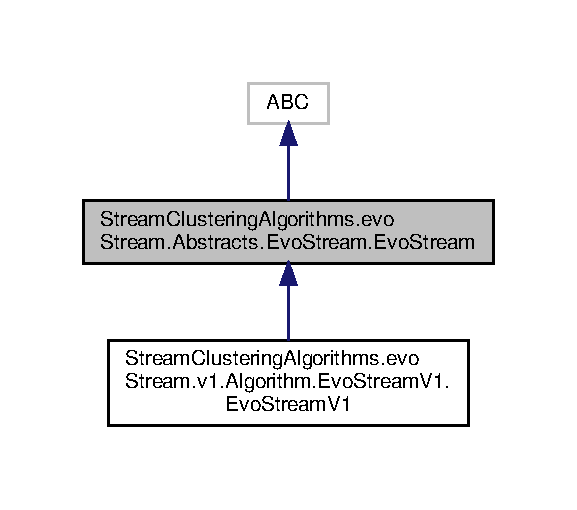
\includegraphics[width=277pt]{classStreamClusteringAlgorithms_1_1evoStream_1_1Abstracts_1_1EvoStream_1_1EvoStream__inherit__graph}
\end{center}
\end{figure}


Collaboration diagram for Stream\+Clustering\+Algorithms.\+evo\+Stream.\+Abstracts.\+Evo\+Stream.\+Evo\+Stream\+:\nopagebreak
\begin{figure}[H]
\begin{center}
\leavevmode
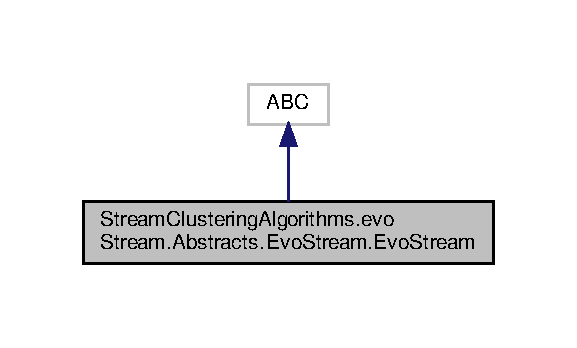
\includegraphics[width=277pt]{classStreamClusteringAlgorithms_1_1evoStream_1_1Abstracts_1_1EvoStream_1_1EvoStream__coll__graph}
\end{center}
\end{figure}
\subsection*{Public Member Functions}
\begin{DoxyCompactItemize}
\item 
def \hyperlink{classStreamClusteringAlgorithms_1_1evoStream_1_1Abstracts_1_1EvoStream_1_1EvoStream_a8cf745b0150af17c433357568e760d3e}{\+\_\+\+\_\+init\+\_\+\+\_\+} (self, args, kwargs)
\end{DoxyCompactItemize}


\subsection{Detailed Description}
Abstract base class for \hyperlink{classStreamClusteringAlgorithms_1_1evoStream_1_1Abstracts_1_1EvoStream_1_1EvoStream}{Evo\+Stream} Algorithm. 

\subsection{Constructor \& Destructor Documentation}
\mbox{\Hypertarget{classStreamClusteringAlgorithms_1_1evoStream_1_1Abstracts_1_1EvoStream_1_1EvoStream_a8cf745b0150af17c433357568e760d3e}\label{classStreamClusteringAlgorithms_1_1evoStream_1_1Abstracts_1_1EvoStream_1_1EvoStream_a8cf745b0150af17c433357568e760d3e}} 
\index{Stream\+Clustering\+Algorithms\+::evo\+Stream\+::\+Abstracts\+::\+Evo\+Stream\+::\+Evo\+Stream@{Stream\+Clustering\+Algorithms\+::evo\+Stream\+::\+Abstracts\+::\+Evo\+Stream\+::\+Evo\+Stream}!\+\_\+\+\_\+init\+\_\+\+\_\+@{\+\_\+\+\_\+init\+\_\+\+\_\+}}
\index{\+\_\+\+\_\+init\+\_\+\+\_\+@{\+\_\+\+\_\+init\+\_\+\+\_\+}!Stream\+Clustering\+Algorithms\+::evo\+Stream\+::\+Abstracts\+::\+Evo\+Stream\+::\+Evo\+Stream@{Stream\+Clustering\+Algorithms\+::evo\+Stream\+::\+Abstracts\+::\+Evo\+Stream\+::\+Evo\+Stream}}
\subsubsection{\texorpdfstring{\+\_\+\+\_\+init\+\_\+\+\_\+()}{\_\_init\_\_()}}
{\footnotesize\ttfamily def Stream\+Clustering\+Algorithms.\+evo\+Stream.\+Abstracts.\+Evo\+Stream.\+Evo\+Stream.\+\_\+\+\_\+init\+\_\+\+\_\+ (\begin{DoxyParamCaption}\item[{}]{self,  }\item[{}]{args,  }\item[{}]{kwargs }\end{DoxyParamCaption})}



The documentation for this class was generated from the following file\+:\begin{DoxyCompactItemize}
\item 
evo\+Stream/\+Abstracts/\hyperlink{EvoStream_8py}{Evo\+Stream.\+py}\end{DoxyCompactItemize}

\hypertarget{classStreamClusteringAlgorithms_1_1evoStream_1_1v1_1_1Algorithm_1_1EvoStreamV1_1_1EvoStreamV1}{}\section{Stream\+Clustering\+Algorithms.\+evo\+Stream.\+v1.\+Algorithm.\+Evo\+Stream\+V1.\+Evo\+Stream\+V1 Class Reference}
\label{classStreamClusteringAlgorithms_1_1evoStream_1_1v1_1_1Algorithm_1_1EvoStreamV1_1_1EvoStreamV1}\index{Stream\+Clustering\+Algorithms.\+evo\+Stream.\+v1.\+Algorithm.\+Evo\+Stream\+V1.\+Evo\+Stream\+V1@{Stream\+Clustering\+Algorithms.\+evo\+Stream.\+v1.\+Algorithm.\+Evo\+Stream\+V1.\+Evo\+Stream\+V1}}


Inheritance diagram for Stream\+Clustering\+Algorithms.\+evo\+Stream.\+v1.\+Algorithm.\+Evo\+Stream\+V1.\+Evo\+Stream\+V1\+:\nopagebreak
\begin{figure}[H]
\begin{center}
\leavevmode
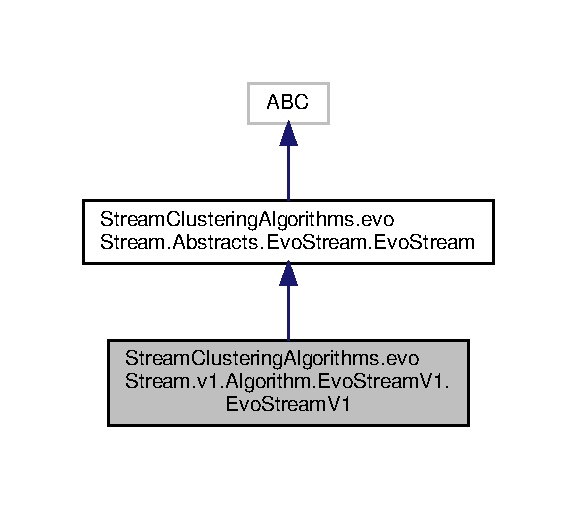
\includegraphics[width=277pt]{classStreamClusteringAlgorithms_1_1evoStream_1_1v1_1_1Algorithm_1_1EvoStreamV1_1_1EvoStreamV1__inherit__graph}
\end{center}
\end{figure}


Collaboration diagram for Stream\+Clustering\+Algorithms.\+evo\+Stream.\+v1.\+Algorithm.\+Evo\+Stream\+V1.\+Evo\+Stream\+V1\+:\nopagebreak
\begin{figure}[H]
\begin{center}
\leavevmode
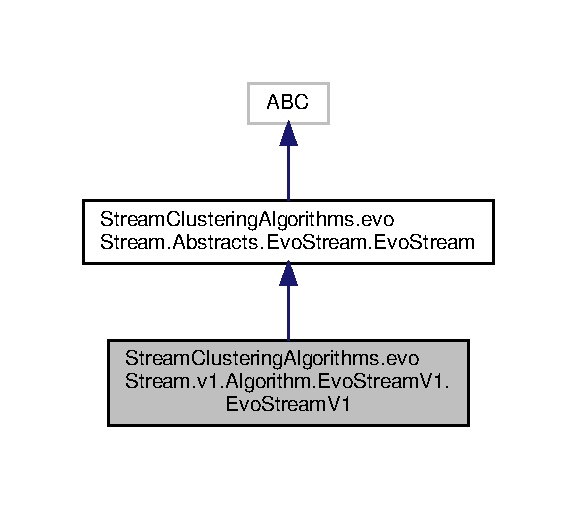
\includegraphics[width=277pt]{classStreamClusteringAlgorithms_1_1evoStream_1_1v1_1_1Algorithm_1_1EvoStreamV1_1_1EvoStreamV1__coll__graph}
\end{center}
\end{figure}
\subsection*{Public Member Functions}
\begin{DoxyCompactItemize}
\item 
def \hyperlink{classStreamClusteringAlgorithms_1_1evoStream_1_1v1_1_1Algorithm_1_1EvoStreamV1_1_1EvoStreamV1_a267ae54d21a6d55321f32dcdd62439aa}{\+\_\+\+\_\+init\+\_\+\+\_\+} (self, args, kwargs)
\item 
def \hyperlink{classStreamClusteringAlgorithms_1_1evoStream_1_1v1_1_1Algorithm_1_1EvoStreamV1_1_1EvoStreamV1_a9533e30378b9198d1afacb7f30796cb5}{update\+\_\+cleanup\+\_\+interval} (self, \hyperlink{classStreamClusteringAlgorithms_1_1evoStream_1_1v1_1_1Algorithm_1_1EvoStreamV1_1_1EvoStreamV1_a46771a05845bae3fc47e2b5a2dc35a9b}{cleanup\+\_\+interval})
\begin{DoxyCompactList}\small\item\em M\+O\+D\+U\+LE F\+OR C\+L\+E\+A\+N-\/\+UP A\+D\+A\+P\+T\+I\+V\+I\+TY. \end{DoxyCompactList}\item 
def \hyperlink{classStreamClusteringAlgorithms_1_1evoStream_1_1v1_1_1Algorithm_1_1EvoStreamV1_1_1EvoStreamV1_a993300bd3531f41834ac0eda9f78c021}{update\+\_\+weights} (self)
\item 
def \hyperlink{classStreamClusteringAlgorithms_1_1evoStream_1_1v1_1_1Algorithm_1_1EvoStreamV1_1_1EvoStreamV1_a519bc4af98ff4b3223439b266d67ab7b}{clean\+\_\+up} (self)
\item 
def \hyperlink{classStreamClusteringAlgorithms_1_1evoStream_1_1v1_1_1Algorithm_1_1EvoStreamV1_1_1EvoStreamV1_ab73522db04392f0469b83d6e01e7f3ac}{get\+\_\+distance\+\_\+vector} (self, mc)
\item 
def \hyperlink{classStreamClusteringAlgorithms_1_1evoStream_1_1v1_1_1Algorithm_1_1EvoStreamV1_1_1EvoStreamV1_ac8fc05e3dcf3c265704f61b825fd82cb}{insert} (self, distances, mc)
\begin{DoxyCompactList}\small\item\em A method that absorbs observation or creates new microcluster. \end{DoxyCompactList}\item 
def \hyperlink{classStreamClusteringAlgorithms_1_1evoStream_1_1v1_1_1Algorithm_1_1EvoStreamV1_1_1EvoStreamV1_a14b9ea4cd658b3bd85569fc256c07612}{cluster} (self, input\+\_\+data)
\begin{DoxyCompactList}\small\item\em A method that creates new microcluster from given input data and inserts to set according to principles of algorithm. \end{DoxyCompactList}\item 
def \hyperlink{classStreamClusteringAlgorithms_1_1evoStream_1_1v1_1_1Algorithm_1_1EvoStreamV1_1_1EvoStreamV1_af3acc41c758a42dac3d09c4d10812ac4}{initialize} (self)
\begin{DoxyCompactList}\small\item\em Randomly chosen M\+A\+C\+RO cluster P\+O\+P\+U\+L\+A\+T\+I\+ON initialization according to defined population size. \end{DoxyCompactList}\item 
def \hyperlink{classStreamClusteringAlgorithms_1_1evoStream_1_1v1_1_1Algorithm_1_1EvoStreamV1_1_1EvoStreamV1_aa5f1b3700b15e2d0d911ab14e6ebffed}{get\+\_\+microclusters} (self)
\item 
def \hyperlink{classStreamClusteringAlgorithms_1_1evoStream_1_1v1_1_1Algorithm_1_1EvoStreamV1_1_1EvoStreamV1_a7810a70a249a65ad701050e4b4bdeac9}{get\+\_\+microweights} (self)
\item 
def \hyperlink{classStreamClusteringAlgorithms_1_1evoStream_1_1v1_1_1Algorithm_1_1EvoStreamV1_1_1EvoStreamV1_acd743d25dfe419279d4745884223d464}{get\+\_\+macroclusters} (self)
\item 
def \hyperlink{classStreamClusteringAlgorithms_1_1evoStream_1_1v1_1_1Algorithm_1_1EvoStreamV1_1_1EvoStreamV1_ab99c359576c47f40cccdfa950c76ed40}{get\+\_\+macroweights} (self)
\item 
def \hyperlink{classStreamClusteringAlgorithms_1_1evoStream_1_1v1_1_1Algorithm_1_1EvoStreamV1_1_1EvoStreamV1_a649bb433a054250b3851a8a966fe8a7d}{micro\+\_\+to\+\_\+macro} (self)
\item 
def \hyperlink{classStreamClusteringAlgorithms_1_1evoStream_1_1v1_1_1Algorithm_1_1EvoStreamV1_1_1EvoStreamV1_a1e337e7c8fc00e3fdc4948e5e160e130}{evolution} (self)
\item 
def \hyperlink{classStreamClusteringAlgorithms_1_1evoStream_1_1v1_1_1Algorithm_1_1EvoStreamV1_1_1EvoStreamV1_a61fe2b70ac376c64a2da71cdd64626c2}{recluster} (self, generations)
\item 
def \hyperlink{classStreamClusteringAlgorithms_1_1evoStream_1_1v1_1_1Algorithm_1_1EvoStreamV1_1_1EvoStreamV1_ab24ec0dd2fbbf9b92e897897c5c976da}{get\+\_\+assignment} (self, centres)
\item 
def \hyperlink{classStreamClusteringAlgorithms_1_1evoStream_1_1v1_1_1Algorithm_1_1EvoStreamV1_1_1EvoStreamV1_aba0df9e50e35afaf30e6c21bcb245e3d}{fitness} (self, centres)
\begin{DoxyCompactList}\small\item\em M\+I\+C\+RO to M\+A\+C\+RO A\+S\+S\+I\+G\+N\+M\+E\+NT I\+N\+D\+E\+X\+ES. \end{DoxyCompactList}\item 
def \hyperlink{classStreamClusteringAlgorithms_1_1evoStream_1_1v1_1_1Algorithm_1_1EvoStreamV1_1_1EvoStreamV1_ad63288667a313d001ee6471dafb93553}{calculate\+\_\+fitness} (self)
\item 
def \hyperlink{classStreamClusteringAlgorithms_1_1evoStream_1_1v1_1_1Algorithm_1_1EvoStreamV1_1_1EvoStreamV1_a490fb3a7a255b6008e1e35e35e058480}{selection} (self, algorithm=\char`\"{}roulette\char`\"{})
\item 
def \hyperlink{classStreamClusteringAlgorithms_1_1evoStream_1_1v1_1_1Algorithm_1_1EvoStreamV1_1_1EvoStreamV1_aa754839b3295d3e955d1411e6be10f19}{crossing\+\_\+over} (self, selections, algorithm=\char`\"{}nebilimolumolcmedimki\char`\"{})
\begin{DoxyCompactList}\small\item\em The method that makes cross-\/over on selected fittest 2 macroclusters. \end{DoxyCompactList}\item 
def \hyperlink{classStreamClusteringAlgorithms_1_1evoStream_1_1v1_1_1Algorithm_1_1EvoStreamV1_1_1EvoStreamV1_a536bf586b720f9b5f6c628c44ceb65f3}{mutation} (self, selections)
\begin{DoxyCompactList}\small\item\em A method that mutates selection values. \end{DoxyCompactList}\item 
def \hyperlink{classStreamClusteringAlgorithms_1_1evoStream_1_1v1_1_1Algorithm_1_1EvoStreamV1_1_1EvoStreamV1_aad90f79618d21685408d625ebfe2b98f}{predict} (self, dataset)
\begin{DoxyCompactList}\small\item\em A method that predicts cluster id according to existing centroids in time, relatively . \end{DoxyCompactList}\item 
def \hyperlink{classStreamClusteringAlgorithms_1_1evoStream_1_1v1_1_1Algorithm_1_1EvoStreamV1_1_1EvoStreamV1_acb5a55416fee376bb40664e8292eb679}{fit} (self, dataset)
\begin{DoxyCompactList}\small\item\em Training. \end{DoxyCompactList}\end{DoxyCompactItemize}
\subsection*{Public Attributes}
\begin{DoxyCompactItemize}
\item 
\hyperlink{classStreamClusteringAlgorithms_1_1evoStream_1_1v1_1_1Algorithm_1_1EvoStreamV1_1_1EvoStreamV1_ac805f8978600ec627155602f0a300acb}{radius}
\begin{DoxyCompactList}\small\item\em Radius value for cluster. \end{DoxyCompactList}\item 
\hyperlink{classStreamClusteringAlgorithms_1_1evoStream_1_1v1_1_1Algorithm_1_1EvoStreamV1_1_1EvoStreamV1_ad946d36cc9c641fccdeaf3535ffbd92c}{decay\+\_\+rate}
\begin{DoxyCompactList}\small\item\em Decay rate. \end{DoxyCompactList}\item 
\hyperlink{classStreamClusteringAlgorithms_1_1evoStream_1_1v1_1_1Algorithm_1_1EvoStreamV1_1_1EvoStreamV1_a46771a05845bae3fc47e2b5a2dc35a9b}{cleanup\+\_\+interval}
\begin{DoxyCompactList}\small\item\em Cleanup interval. \end{DoxyCompactList}\item 
\hyperlink{classStreamClusteringAlgorithms_1_1evoStream_1_1v1_1_1Algorithm_1_1EvoStreamV1_1_1EvoStreamV1_adcee0667881d3fa73fecfe7c42874261}{k}
\begin{DoxyCompactList}\small\item\em Number of clusters. \end{DoxyCompactList}\item 
\hyperlink{classStreamClusteringAlgorithms_1_1evoStream_1_1v1_1_1Algorithm_1_1EvoStreamV1_1_1EvoStreamV1_a2418409c6f9e3c80fe0998aeff08f3d2}{omega}
\begin{DoxyCompactList}\small\item\em Omega calculation. \end{DoxyCompactList}\item 
\hyperlink{classStreamClusteringAlgorithms_1_1evoStream_1_1v1_1_1Algorithm_1_1EvoStreamV1_1_1EvoStreamV1_a55bc61778be7d7993c378abd0da8afe0}{crossover\+\_\+rate}
\begin{DoxyCompactList}\small\item\em GA P\+A\+R\+A\+M\+E\+T\+E\+RS Crossover rate. \end{DoxyCompactList}\item 
\hyperlink{classStreamClusteringAlgorithms_1_1evoStream_1_1v1_1_1Algorithm_1_1EvoStreamV1_1_1EvoStreamV1_a193d4b167e403f3fb27c446d03273edd}{mutation\+\_\+rate}
\begin{DoxyCompactList}\small\item\em Mutation rate. \end{DoxyCompactList}\item 
\hyperlink{classStreamClusteringAlgorithms_1_1evoStream_1_1v1_1_1Algorithm_1_1EvoStreamV1_1_1EvoStreamV1_a199eaed6b415bc040518dcc441f93d83}{population\+\_\+size}
\begin{DoxyCompactList}\small\item\em Population size. \end{DoxyCompactList}\item 
\hyperlink{classStreamClusteringAlgorithms_1_1evoStream_1_1v1_1_1Algorithm_1_1EvoStreamV1_1_1EvoStreamV1_ab86e66908b70ceb1ac38ff1708d3c45c}{initialize\+\_\+after}
\begin{DoxyCompactList}\small\item\em Initalization after x number of inputs. \end{DoxyCompactList}\item 
\hyperlink{classStreamClusteringAlgorithms_1_1evoStream_1_1v1_1_1Algorithm_1_1EvoStreamV1_1_1EvoStreamV1_ac45c8bef514493d96156a59a78af124f}{recluster\+\_\+generations}
\begin{DoxyCompactList}\small\item\em Recluster generation interval parameters. \end{DoxyCompactList}\item 
\hyperlink{classStreamClusteringAlgorithms_1_1evoStream_1_1v1_1_1Algorithm_1_1EvoStreamV1_1_1EvoStreamV1_aeda962414bb181b7032317483d8df1ad}{dict}
\item 
\hyperlink{classStreamClusteringAlgorithms_1_1evoStream_1_1v1_1_1Algorithm_1_1EvoStreamV1_1_1EvoStreamV1_a432355bc9e64785657d96f63023169ee}{init}
\item 
\hyperlink{classStreamClusteringAlgorithms_1_1evoStream_1_1v1_1_1Algorithm_1_1EvoStreamV1_1_1EvoStreamV1_a639c6ab2cd9da9fa4975cb212a305740}{init\+\_\+time}
\item 
\hyperlink{classStreamClusteringAlgorithms_1_1evoStream_1_1v1_1_1Algorithm_1_1EvoStreamV1_1_1EvoStreamV1_a0777f8aaf2a42d9c7fc6abdb2e1a7645}{warming\+\_\+current}
\item 
\hyperlink{classStreamClusteringAlgorithms_1_1evoStream_1_1v1_1_1Algorithm_1_1EvoStreamV1_1_1EvoStreamV1_a1008e3ae665d3d1a9e06ce20b21685c4}{warming\+\_\+instance\+\_\+count}
\item 
\hyperlink{classStreamClusteringAlgorithms_1_1evoStream_1_1v1_1_1Algorithm_1_1EvoStreamV1_1_1EvoStreamV1_a63bf203d96c31a13ad645ef6dd2e2619}{uptodate}
\item 
\hyperlink{classStreamClusteringAlgorithms_1_1evoStream_1_1v1_1_1Algorithm_1_1EvoStreamV1_1_1EvoStreamV1_ab3bb06f047c2d39dc2f44a7aca98f91e}{current\+\_\+time}
\item 
\hyperlink{classStreamClusteringAlgorithms_1_1evoStream_1_1v1_1_1Algorithm_1_1EvoStreamV1_1_1EvoStreamV1_a9410090db1374e7d0f116dde1a177df2}{macro\+\_\+fitness}
\item 
\hyperlink{classStreamClusteringAlgorithms_1_1evoStream_1_1v1_1_1Algorithm_1_1EvoStreamV1_1_1EvoStreamV1_a17f1b10fbbed67abac36775b53ab8525}{micro\+\_\+clusters}
\item 
\hyperlink{classStreamClusteringAlgorithms_1_1evoStream_1_1v1_1_1Algorithm_1_1EvoStreamV1_1_1EvoStreamV1_ac7a5dd9d76aa16832e507782e14284d8}{macro\+\_\+clusters}
\item 
\hyperlink{classStreamClusteringAlgorithms_1_1evoStream_1_1v1_1_1Algorithm_1_1EvoStreamV1_1_1EvoStreamV1_a1335bbb4976a282c55b7d23631fadc4f}{utils}
\end{DoxyCompactItemize}


\subsection{Constructor \& Destructor Documentation}
\mbox{\Hypertarget{classStreamClusteringAlgorithms_1_1evoStream_1_1v1_1_1Algorithm_1_1EvoStreamV1_1_1EvoStreamV1_a267ae54d21a6d55321f32dcdd62439aa}\label{classStreamClusteringAlgorithms_1_1evoStream_1_1v1_1_1Algorithm_1_1EvoStreamV1_1_1EvoStreamV1_a267ae54d21a6d55321f32dcdd62439aa}} 
\index{Stream\+Clustering\+Algorithms\+::evo\+Stream\+::v1\+::\+Algorithm\+::\+Evo\+Stream\+V1\+::\+Evo\+Stream\+V1@{Stream\+Clustering\+Algorithms\+::evo\+Stream\+::v1\+::\+Algorithm\+::\+Evo\+Stream\+V1\+::\+Evo\+Stream\+V1}!\+\_\+\+\_\+init\+\_\+\+\_\+@{\+\_\+\+\_\+init\+\_\+\+\_\+}}
\index{\+\_\+\+\_\+init\+\_\+\+\_\+@{\+\_\+\+\_\+init\+\_\+\+\_\+}!Stream\+Clustering\+Algorithms\+::evo\+Stream\+::v1\+::\+Algorithm\+::\+Evo\+Stream\+V1\+::\+Evo\+Stream\+V1@{Stream\+Clustering\+Algorithms\+::evo\+Stream\+::v1\+::\+Algorithm\+::\+Evo\+Stream\+V1\+::\+Evo\+Stream\+V1}}
\subsubsection{\texorpdfstring{\+\_\+\+\_\+init\+\_\+\+\_\+()}{\_\_init\_\_()}}
{\footnotesize\ttfamily def Stream\+Clustering\+Algorithms.\+evo\+Stream.\+v1.\+Algorithm.\+Evo\+Stream\+V1.\+Evo\+Stream\+V1.\+\_\+\+\_\+init\+\_\+\+\_\+ (\begin{DoxyParamCaption}\item[{}]{self,  }\item[{}]{args,  }\item[{}]{kwargs }\end{DoxyParamCaption})}



\subsection{Member Function Documentation}
\mbox{\Hypertarget{classStreamClusteringAlgorithms_1_1evoStream_1_1v1_1_1Algorithm_1_1EvoStreamV1_1_1EvoStreamV1_ad63288667a313d001ee6471dafb93553}\label{classStreamClusteringAlgorithms_1_1evoStream_1_1v1_1_1Algorithm_1_1EvoStreamV1_1_1EvoStreamV1_ad63288667a313d001ee6471dafb93553}} 
\index{Stream\+Clustering\+Algorithms\+::evo\+Stream\+::v1\+::\+Algorithm\+::\+Evo\+Stream\+V1\+::\+Evo\+Stream\+V1@{Stream\+Clustering\+Algorithms\+::evo\+Stream\+::v1\+::\+Algorithm\+::\+Evo\+Stream\+V1\+::\+Evo\+Stream\+V1}!calculate\+\_\+fitness@{calculate\+\_\+fitness}}
\index{calculate\+\_\+fitness@{calculate\+\_\+fitness}!Stream\+Clustering\+Algorithms\+::evo\+Stream\+::v1\+::\+Algorithm\+::\+Evo\+Stream\+V1\+::\+Evo\+Stream\+V1@{Stream\+Clustering\+Algorithms\+::evo\+Stream\+::v1\+::\+Algorithm\+::\+Evo\+Stream\+V1\+::\+Evo\+Stream\+V1}}
\subsubsection{\texorpdfstring{calculate\+\_\+fitness()}{calculate\_fitness()}}
{\footnotesize\ttfamily def Stream\+Clustering\+Algorithms.\+evo\+Stream.\+v1.\+Algorithm.\+Evo\+Stream\+V1.\+Evo\+Stream\+V1.\+calculate\+\_\+fitness (\begin{DoxyParamCaption}\item[{}]{self }\end{DoxyParamCaption})}

\mbox{\Hypertarget{classStreamClusteringAlgorithms_1_1evoStream_1_1v1_1_1Algorithm_1_1EvoStreamV1_1_1EvoStreamV1_a519bc4af98ff4b3223439b266d67ab7b}\label{classStreamClusteringAlgorithms_1_1evoStream_1_1v1_1_1Algorithm_1_1EvoStreamV1_1_1EvoStreamV1_a519bc4af98ff4b3223439b266d67ab7b}} 
\index{Stream\+Clustering\+Algorithms\+::evo\+Stream\+::v1\+::\+Algorithm\+::\+Evo\+Stream\+V1\+::\+Evo\+Stream\+V1@{Stream\+Clustering\+Algorithms\+::evo\+Stream\+::v1\+::\+Algorithm\+::\+Evo\+Stream\+V1\+::\+Evo\+Stream\+V1}!clean\+\_\+up@{clean\+\_\+up}}
\index{clean\+\_\+up@{clean\+\_\+up}!Stream\+Clustering\+Algorithms\+::evo\+Stream\+::v1\+::\+Algorithm\+::\+Evo\+Stream\+V1\+::\+Evo\+Stream\+V1@{Stream\+Clustering\+Algorithms\+::evo\+Stream\+::v1\+::\+Algorithm\+::\+Evo\+Stream\+V1\+::\+Evo\+Stream\+V1}}
\subsubsection{\texorpdfstring{clean\+\_\+up()}{clean\_up()}}
{\footnotesize\ttfamily def Stream\+Clustering\+Algorithms.\+evo\+Stream.\+v1.\+Algorithm.\+Evo\+Stream\+V1.\+Evo\+Stream\+V1.\+clean\+\_\+up (\begin{DoxyParamCaption}\item[{}]{self }\end{DoxyParamCaption})}

\mbox{\Hypertarget{classStreamClusteringAlgorithms_1_1evoStream_1_1v1_1_1Algorithm_1_1EvoStreamV1_1_1EvoStreamV1_a14b9ea4cd658b3bd85569fc256c07612}\label{classStreamClusteringAlgorithms_1_1evoStream_1_1v1_1_1Algorithm_1_1EvoStreamV1_1_1EvoStreamV1_a14b9ea4cd658b3bd85569fc256c07612}} 
\index{Stream\+Clustering\+Algorithms\+::evo\+Stream\+::v1\+::\+Algorithm\+::\+Evo\+Stream\+V1\+::\+Evo\+Stream\+V1@{Stream\+Clustering\+Algorithms\+::evo\+Stream\+::v1\+::\+Algorithm\+::\+Evo\+Stream\+V1\+::\+Evo\+Stream\+V1}!cluster@{cluster}}
\index{cluster@{cluster}!Stream\+Clustering\+Algorithms\+::evo\+Stream\+::v1\+::\+Algorithm\+::\+Evo\+Stream\+V1\+::\+Evo\+Stream\+V1@{Stream\+Clustering\+Algorithms\+::evo\+Stream\+::v1\+::\+Algorithm\+::\+Evo\+Stream\+V1\+::\+Evo\+Stream\+V1}}
\subsubsection{\texorpdfstring{cluster()}{cluster()}}
{\footnotesize\ttfamily def Stream\+Clustering\+Algorithms.\+evo\+Stream.\+v1.\+Algorithm.\+Evo\+Stream\+V1.\+Evo\+Stream\+V1.\+cluster (\begin{DoxyParamCaption}\item[{}]{self,  }\item[{}]{input\+\_\+data }\end{DoxyParamCaption})}



A method that creates new microcluster from given input data and inserts to set according to principles of algorithm. 


\begin{DoxyParams}{Parameters}
{\em input\+\_\+data} & Vector, value, centroid etc. \\
\hline
\end{DoxyParams}
\begin{DoxyReturn}{Returns}
\+: None 
\end{DoxyReturn}
\mbox{\Hypertarget{classStreamClusteringAlgorithms_1_1evoStream_1_1v1_1_1Algorithm_1_1EvoStreamV1_1_1EvoStreamV1_aa754839b3295d3e955d1411e6be10f19}\label{classStreamClusteringAlgorithms_1_1evoStream_1_1v1_1_1Algorithm_1_1EvoStreamV1_1_1EvoStreamV1_aa754839b3295d3e955d1411e6be10f19}} 
\index{Stream\+Clustering\+Algorithms\+::evo\+Stream\+::v1\+::\+Algorithm\+::\+Evo\+Stream\+V1\+::\+Evo\+Stream\+V1@{Stream\+Clustering\+Algorithms\+::evo\+Stream\+::v1\+::\+Algorithm\+::\+Evo\+Stream\+V1\+::\+Evo\+Stream\+V1}!crossing\+\_\+over@{crossing\+\_\+over}}
\index{crossing\+\_\+over@{crossing\+\_\+over}!Stream\+Clustering\+Algorithms\+::evo\+Stream\+::v1\+::\+Algorithm\+::\+Evo\+Stream\+V1\+::\+Evo\+Stream\+V1@{Stream\+Clustering\+Algorithms\+::evo\+Stream\+::v1\+::\+Algorithm\+::\+Evo\+Stream\+V1\+::\+Evo\+Stream\+V1}}
\subsubsection{\texorpdfstring{crossing\+\_\+over()}{crossing\_over()}}
{\footnotesize\ttfamily def Stream\+Clustering\+Algorithms.\+evo\+Stream.\+v1.\+Algorithm.\+Evo\+Stream\+V1.\+Evo\+Stream\+V1.\+crossing\+\_\+over (\begin{DoxyParamCaption}\item[{}]{self,  }\item[{}]{selections,  }\item[{}]{algorithm = {\ttfamily \char`\"{}nebilimolumolcmedimki\char`\"{}} }\end{DoxyParamCaption})}



The method that makes cross-\/over on selected fittest 2 macroclusters. 


\begin{DoxyParams}{Parameters}
{\em selections} & Selected gene indexes \\
\hline
{\em algorithm} & future improvement alg switching \\
\hline
\end{DoxyParams}
\begin{DoxyReturn}{Returns}
\+: 
\end{DoxyReturn}
\mbox{\Hypertarget{classStreamClusteringAlgorithms_1_1evoStream_1_1v1_1_1Algorithm_1_1EvoStreamV1_1_1EvoStreamV1_a1e337e7c8fc00e3fdc4948e5e160e130}\label{classStreamClusteringAlgorithms_1_1evoStream_1_1v1_1_1Algorithm_1_1EvoStreamV1_1_1EvoStreamV1_a1e337e7c8fc00e3fdc4948e5e160e130}} 
\index{Stream\+Clustering\+Algorithms\+::evo\+Stream\+::v1\+::\+Algorithm\+::\+Evo\+Stream\+V1\+::\+Evo\+Stream\+V1@{Stream\+Clustering\+Algorithms\+::evo\+Stream\+::v1\+::\+Algorithm\+::\+Evo\+Stream\+V1\+::\+Evo\+Stream\+V1}!evolution@{evolution}}
\index{evolution@{evolution}!Stream\+Clustering\+Algorithms\+::evo\+Stream\+::v1\+::\+Algorithm\+::\+Evo\+Stream\+V1\+::\+Evo\+Stream\+V1@{Stream\+Clustering\+Algorithms\+::evo\+Stream\+::v1\+::\+Algorithm\+::\+Evo\+Stream\+V1\+::\+Evo\+Stream\+V1}}
\subsubsection{\texorpdfstring{evolution()}{evolution()}}
{\footnotesize\ttfamily def Stream\+Clustering\+Algorithms.\+evo\+Stream.\+v1.\+Algorithm.\+Evo\+Stream\+V1.\+Evo\+Stream\+V1.\+evolution (\begin{DoxyParamCaption}\item[{}]{self }\end{DoxyParamCaption})}

\mbox{\Hypertarget{classStreamClusteringAlgorithms_1_1evoStream_1_1v1_1_1Algorithm_1_1EvoStreamV1_1_1EvoStreamV1_acb5a55416fee376bb40664e8292eb679}\label{classStreamClusteringAlgorithms_1_1evoStream_1_1v1_1_1Algorithm_1_1EvoStreamV1_1_1EvoStreamV1_acb5a55416fee376bb40664e8292eb679}} 
\index{Stream\+Clustering\+Algorithms\+::evo\+Stream\+::v1\+::\+Algorithm\+::\+Evo\+Stream\+V1\+::\+Evo\+Stream\+V1@{Stream\+Clustering\+Algorithms\+::evo\+Stream\+::v1\+::\+Algorithm\+::\+Evo\+Stream\+V1\+::\+Evo\+Stream\+V1}!fit@{fit}}
\index{fit@{fit}!Stream\+Clustering\+Algorithms\+::evo\+Stream\+::v1\+::\+Algorithm\+::\+Evo\+Stream\+V1\+::\+Evo\+Stream\+V1@{Stream\+Clustering\+Algorithms\+::evo\+Stream\+::v1\+::\+Algorithm\+::\+Evo\+Stream\+V1\+::\+Evo\+Stream\+V1}}
\subsubsection{\texorpdfstring{fit()}{fit()}}
{\footnotesize\ttfamily def Stream\+Clustering\+Algorithms.\+evo\+Stream.\+v1.\+Algorithm.\+Evo\+Stream\+V1.\+Evo\+Stream\+V1.\+fit (\begin{DoxyParamCaption}\item[{}]{self,  }\item[{}]{dataset }\end{DoxyParamCaption})}



Training. 


\begin{DoxyParams}{Parameters}
{\em dataset} & \\
\hline
\end{DoxyParams}
\begin{DoxyReturn}{Returns}
\+: 
\end{DoxyReturn}
\mbox{\Hypertarget{classStreamClusteringAlgorithms_1_1evoStream_1_1v1_1_1Algorithm_1_1EvoStreamV1_1_1EvoStreamV1_aba0df9e50e35afaf30e6c21bcb245e3d}\label{classStreamClusteringAlgorithms_1_1evoStream_1_1v1_1_1Algorithm_1_1EvoStreamV1_1_1EvoStreamV1_aba0df9e50e35afaf30e6c21bcb245e3d}} 
\index{Stream\+Clustering\+Algorithms\+::evo\+Stream\+::v1\+::\+Algorithm\+::\+Evo\+Stream\+V1\+::\+Evo\+Stream\+V1@{Stream\+Clustering\+Algorithms\+::evo\+Stream\+::v1\+::\+Algorithm\+::\+Evo\+Stream\+V1\+::\+Evo\+Stream\+V1}!fitness@{fitness}}
\index{fitness@{fitness}!Stream\+Clustering\+Algorithms\+::evo\+Stream\+::v1\+::\+Algorithm\+::\+Evo\+Stream\+V1\+::\+Evo\+Stream\+V1@{Stream\+Clustering\+Algorithms\+::evo\+Stream\+::v1\+::\+Algorithm\+::\+Evo\+Stream\+V1\+::\+Evo\+Stream\+V1}}
\subsubsection{\texorpdfstring{fitness()}{fitness()}}
{\footnotesize\ttfamily def Stream\+Clustering\+Algorithms.\+evo\+Stream.\+v1.\+Algorithm.\+Evo\+Stream\+V1.\+Evo\+Stream\+V1.\+fitness (\begin{DoxyParamCaption}\item[{}]{self,  }\item[{}]{centres }\end{DoxyParamCaption})}



M\+I\+C\+RO to M\+A\+C\+RO A\+S\+S\+I\+G\+N\+M\+E\+NT I\+N\+D\+E\+X\+ES. 


\begin{DoxyParams}{Parameters}
{\em centres} & \\
\hline
\end{DoxyParams}
\begin{DoxyReturn}{Returns}
\+: 
\end{DoxyReturn}
\mbox{\Hypertarget{classStreamClusteringAlgorithms_1_1evoStream_1_1v1_1_1Algorithm_1_1EvoStreamV1_1_1EvoStreamV1_ab24ec0dd2fbbf9b92e897897c5c976da}\label{classStreamClusteringAlgorithms_1_1evoStream_1_1v1_1_1Algorithm_1_1EvoStreamV1_1_1EvoStreamV1_ab24ec0dd2fbbf9b92e897897c5c976da}} 
\index{Stream\+Clustering\+Algorithms\+::evo\+Stream\+::v1\+::\+Algorithm\+::\+Evo\+Stream\+V1\+::\+Evo\+Stream\+V1@{Stream\+Clustering\+Algorithms\+::evo\+Stream\+::v1\+::\+Algorithm\+::\+Evo\+Stream\+V1\+::\+Evo\+Stream\+V1}!get\+\_\+assignment@{get\+\_\+assignment}}
\index{get\+\_\+assignment@{get\+\_\+assignment}!Stream\+Clustering\+Algorithms\+::evo\+Stream\+::v1\+::\+Algorithm\+::\+Evo\+Stream\+V1\+::\+Evo\+Stream\+V1@{Stream\+Clustering\+Algorithms\+::evo\+Stream\+::v1\+::\+Algorithm\+::\+Evo\+Stream\+V1\+::\+Evo\+Stream\+V1}}
\subsubsection{\texorpdfstring{get\+\_\+assignment()}{get\_assignment()}}
{\footnotesize\ttfamily def Stream\+Clustering\+Algorithms.\+evo\+Stream.\+v1.\+Algorithm.\+Evo\+Stream\+V1.\+Evo\+Stream\+V1.\+get\+\_\+assignment (\begin{DoxyParamCaption}\item[{}]{self,  }\item[{}]{centres }\end{DoxyParamCaption})}

\mbox{\Hypertarget{classStreamClusteringAlgorithms_1_1evoStream_1_1v1_1_1Algorithm_1_1EvoStreamV1_1_1EvoStreamV1_ab73522db04392f0469b83d6e01e7f3ac}\label{classStreamClusteringAlgorithms_1_1evoStream_1_1v1_1_1Algorithm_1_1EvoStreamV1_1_1EvoStreamV1_ab73522db04392f0469b83d6e01e7f3ac}} 
\index{Stream\+Clustering\+Algorithms\+::evo\+Stream\+::v1\+::\+Algorithm\+::\+Evo\+Stream\+V1\+::\+Evo\+Stream\+V1@{Stream\+Clustering\+Algorithms\+::evo\+Stream\+::v1\+::\+Algorithm\+::\+Evo\+Stream\+V1\+::\+Evo\+Stream\+V1}!get\+\_\+distance\+\_\+vector@{get\+\_\+distance\+\_\+vector}}
\index{get\+\_\+distance\+\_\+vector@{get\+\_\+distance\+\_\+vector}!Stream\+Clustering\+Algorithms\+::evo\+Stream\+::v1\+::\+Algorithm\+::\+Evo\+Stream\+V1\+::\+Evo\+Stream\+V1@{Stream\+Clustering\+Algorithms\+::evo\+Stream\+::v1\+::\+Algorithm\+::\+Evo\+Stream\+V1\+::\+Evo\+Stream\+V1}}
\subsubsection{\texorpdfstring{get\+\_\+distance\+\_\+vector()}{get\_distance\_vector()}}
{\footnotesize\ttfamily def Stream\+Clustering\+Algorithms.\+evo\+Stream.\+v1.\+Algorithm.\+Evo\+Stream\+V1.\+Evo\+Stream\+V1.\+get\+\_\+distance\+\_\+vector (\begin{DoxyParamCaption}\item[{}]{self,  }\item[{}]{mc }\end{DoxyParamCaption})}

\mbox{\Hypertarget{classStreamClusteringAlgorithms_1_1evoStream_1_1v1_1_1Algorithm_1_1EvoStreamV1_1_1EvoStreamV1_acd743d25dfe419279d4745884223d464}\label{classStreamClusteringAlgorithms_1_1evoStream_1_1v1_1_1Algorithm_1_1EvoStreamV1_1_1EvoStreamV1_acd743d25dfe419279d4745884223d464}} 
\index{Stream\+Clustering\+Algorithms\+::evo\+Stream\+::v1\+::\+Algorithm\+::\+Evo\+Stream\+V1\+::\+Evo\+Stream\+V1@{Stream\+Clustering\+Algorithms\+::evo\+Stream\+::v1\+::\+Algorithm\+::\+Evo\+Stream\+V1\+::\+Evo\+Stream\+V1}!get\+\_\+macroclusters@{get\+\_\+macroclusters}}
\index{get\+\_\+macroclusters@{get\+\_\+macroclusters}!Stream\+Clustering\+Algorithms\+::evo\+Stream\+::v1\+::\+Algorithm\+::\+Evo\+Stream\+V1\+::\+Evo\+Stream\+V1@{Stream\+Clustering\+Algorithms\+::evo\+Stream\+::v1\+::\+Algorithm\+::\+Evo\+Stream\+V1\+::\+Evo\+Stream\+V1}}
\subsubsection{\texorpdfstring{get\+\_\+macroclusters()}{get\_macroclusters()}}
{\footnotesize\ttfamily def Stream\+Clustering\+Algorithms.\+evo\+Stream.\+v1.\+Algorithm.\+Evo\+Stream\+V1.\+Evo\+Stream\+V1.\+get\+\_\+macroclusters (\begin{DoxyParamCaption}\item[{}]{self }\end{DoxyParamCaption})}

\mbox{\Hypertarget{classStreamClusteringAlgorithms_1_1evoStream_1_1v1_1_1Algorithm_1_1EvoStreamV1_1_1EvoStreamV1_ab99c359576c47f40cccdfa950c76ed40}\label{classStreamClusteringAlgorithms_1_1evoStream_1_1v1_1_1Algorithm_1_1EvoStreamV1_1_1EvoStreamV1_ab99c359576c47f40cccdfa950c76ed40}} 
\index{Stream\+Clustering\+Algorithms\+::evo\+Stream\+::v1\+::\+Algorithm\+::\+Evo\+Stream\+V1\+::\+Evo\+Stream\+V1@{Stream\+Clustering\+Algorithms\+::evo\+Stream\+::v1\+::\+Algorithm\+::\+Evo\+Stream\+V1\+::\+Evo\+Stream\+V1}!get\+\_\+macroweights@{get\+\_\+macroweights}}
\index{get\+\_\+macroweights@{get\+\_\+macroweights}!Stream\+Clustering\+Algorithms\+::evo\+Stream\+::v1\+::\+Algorithm\+::\+Evo\+Stream\+V1\+::\+Evo\+Stream\+V1@{Stream\+Clustering\+Algorithms\+::evo\+Stream\+::v1\+::\+Algorithm\+::\+Evo\+Stream\+V1\+::\+Evo\+Stream\+V1}}
\subsubsection{\texorpdfstring{get\+\_\+macroweights()}{get\_macroweights()}}
{\footnotesize\ttfamily def Stream\+Clustering\+Algorithms.\+evo\+Stream.\+v1.\+Algorithm.\+Evo\+Stream\+V1.\+Evo\+Stream\+V1.\+get\+\_\+macroweights (\begin{DoxyParamCaption}\item[{}]{self }\end{DoxyParamCaption})}

\mbox{\Hypertarget{classStreamClusteringAlgorithms_1_1evoStream_1_1v1_1_1Algorithm_1_1EvoStreamV1_1_1EvoStreamV1_aa5f1b3700b15e2d0d911ab14e6ebffed}\label{classStreamClusteringAlgorithms_1_1evoStream_1_1v1_1_1Algorithm_1_1EvoStreamV1_1_1EvoStreamV1_aa5f1b3700b15e2d0d911ab14e6ebffed}} 
\index{Stream\+Clustering\+Algorithms\+::evo\+Stream\+::v1\+::\+Algorithm\+::\+Evo\+Stream\+V1\+::\+Evo\+Stream\+V1@{Stream\+Clustering\+Algorithms\+::evo\+Stream\+::v1\+::\+Algorithm\+::\+Evo\+Stream\+V1\+::\+Evo\+Stream\+V1}!get\+\_\+microclusters@{get\+\_\+microclusters}}
\index{get\+\_\+microclusters@{get\+\_\+microclusters}!Stream\+Clustering\+Algorithms\+::evo\+Stream\+::v1\+::\+Algorithm\+::\+Evo\+Stream\+V1\+::\+Evo\+Stream\+V1@{Stream\+Clustering\+Algorithms\+::evo\+Stream\+::v1\+::\+Algorithm\+::\+Evo\+Stream\+V1\+::\+Evo\+Stream\+V1}}
\subsubsection{\texorpdfstring{get\+\_\+microclusters()}{get\_microclusters()}}
{\footnotesize\ttfamily def Stream\+Clustering\+Algorithms.\+evo\+Stream.\+v1.\+Algorithm.\+Evo\+Stream\+V1.\+Evo\+Stream\+V1.\+get\+\_\+microclusters (\begin{DoxyParamCaption}\item[{}]{self }\end{DoxyParamCaption})}

\mbox{\Hypertarget{classStreamClusteringAlgorithms_1_1evoStream_1_1v1_1_1Algorithm_1_1EvoStreamV1_1_1EvoStreamV1_a7810a70a249a65ad701050e4b4bdeac9}\label{classStreamClusteringAlgorithms_1_1evoStream_1_1v1_1_1Algorithm_1_1EvoStreamV1_1_1EvoStreamV1_a7810a70a249a65ad701050e4b4bdeac9}} 
\index{Stream\+Clustering\+Algorithms\+::evo\+Stream\+::v1\+::\+Algorithm\+::\+Evo\+Stream\+V1\+::\+Evo\+Stream\+V1@{Stream\+Clustering\+Algorithms\+::evo\+Stream\+::v1\+::\+Algorithm\+::\+Evo\+Stream\+V1\+::\+Evo\+Stream\+V1}!get\+\_\+microweights@{get\+\_\+microweights}}
\index{get\+\_\+microweights@{get\+\_\+microweights}!Stream\+Clustering\+Algorithms\+::evo\+Stream\+::v1\+::\+Algorithm\+::\+Evo\+Stream\+V1\+::\+Evo\+Stream\+V1@{Stream\+Clustering\+Algorithms\+::evo\+Stream\+::v1\+::\+Algorithm\+::\+Evo\+Stream\+V1\+::\+Evo\+Stream\+V1}}
\subsubsection{\texorpdfstring{get\+\_\+microweights()}{get\_microweights()}}
{\footnotesize\ttfamily def Stream\+Clustering\+Algorithms.\+evo\+Stream.\+v1.\+Algorithm.\+Evo\+Stream\+V1.\+Evo\+Stream\+V1.\+get\+\_\+microweights (\begin{DoxyParamCaption}\item[{}]{self }\end{DoxyParamCaption})}

\mbox{\Hypertarget{classStreamClusteringAlgorithms_1_1evoStream_1_1v1_1_1Algorithm_1_1EvoStreamV1_1_1EvoStreamV1_af3acc41c758a42dac3d09c4d10812ac4}\label{classStreamClusteringAlgorithms_1_1evoStream_1_1v1_1_1Algorithm_1_1EvoStreamV1_1_1EvoStreamV1_af3acc41c758a42dac3d09c4d10812ac4}} 
\index{Stream\+Clustering\+Algorithms\+::evo\+Stream\+::v1\+::\+Algorithm\+::\+Evo\+Stream\+V1\+::\+Evo\+Stream\+V1@{Stream\+Clustering\+Algorithms\+::evo\+Stream\+::v1\+::\+Algorithm\+::\+Evo\+Stream\+V1\+::\+Evo\+Stream\+V1}!initialize@{initialize}}
\index{initialize@{initialize}!Stream\+Clustering\+Algorithms\+::evo\+Stream\+::v1\+::\+Algorithm\+::\+Evo\+Stream\+V1\+::\+Evo\+Stream\+V1@{Stream\+Clustering\+Algorithms\+::evo\+Stream\+::v1\+::\+Algorithm\+::\+Evo\+Stream\+V1\+::\+Evo\+Stream\+V1}}
\subsubsection{\texorpdfstring{initialize()}{initialize()}}
{\footnotesize\ttfamily def Stream\+Clustering\+Algorithms.\+evo\+Stream.\+v1.\+Algorithm.\+Evo\+Stream\+V1.\+Evo\+Stream\+V1.\+initialize (\begin{DoxyParamCaption}\item[{}]{self }\end{DoxyParamCaption})}



Randomly chosen M\+A\+C\+RO cluster P\+O\+P\+U\+L\+A\+T\+I\+ON initialization according to defined population size. 

\begin{DoxyReturn}{Returns}
\+: None 
\end{DoxyReturn}
\mbox{\Hypertarget{classStreamClusteringAlgorithms_1_1evoStream_1_1v1_1_1Algorithm_1_1EvoStreamV1_1_1EvoStreamV1_ac8fc05e3dcf3c265704f61b825fd82cb}\label{classStreamClusteringAlgorithms_1_1evoStream_1_1v1_1_1Algorithm_1_1EvoStreamV1_1_1EvoStreamV1_ac8fc05e3dcf3c265704f61b825fd82cb}} 
\index{Stream\+Clustering\+Algorithms\+::evo\+Stream\+::v1\+::\+Algorithm\+::\+Evo\+Stream\+V1\+::\+Evo\+Stream\+V1@{Stream\+Clustering\+Algorithms\+::evo\+Stream\+::v1\+::\+Algorithm\+::\+Evo\+Stream\+V1\+::\+Evo\+Stream\+V1}!insert@{insert}}
\index{insert@{insert}!Stream\+Clustering\+Algorithms\+::evo\+Stream\+::v1\+::\+Algorithm\+::\+Evo\+Stream\+V1\+::\+Evo\+Stream\+V1@{Stream\+Clustering\+Algorithms\+::evo\+Stream\+::v1\+::\+Algorithm\+::\+Evo\+Stream\+V1\+::\+Evo\+Stream\+V1}}
\subsubsection{\texorpdfstring{insert()}{insert()}}
{\footnotesize\ttfamily def Stream\+Clustering\+Algorithms.\+evo\+Stream.\+v1.\+Algorithm.\+Evo\+Stream\+V1.\+Evo\+Stream\+V1.\+insert (\begin{DoxyParamCaption}\item[{}]{self,  }\item[{}]{distances,  }\item[{}]{mc }\end{DoxyParamCaption})}



A method that absorbs observation or creates new microcluster. 


\begin{DoxyParams}{Parameters}
{\em distances} & Distance array to other microclusters \\
\hline
{\em mc} & New coming microcluster object. \\
\hline
\end{DoxyParams}
\begin{DoxyReturn}{Returns}
\+: None 
\end{DoxyReturn}
\mbox{\Hypertarget{classStreamClusteringAlgorithms_1_1evoStream_1_1v1_1_1Algorithm_1_1EvoStreamV1_1_1EvoStreamV1_a649bb433a054250b3851a8a966fe8a7d}\label{classStreamClusteringAlgorithms_1_1evoStream_1_1v1_1_1Algorithm_1_1EvoStreamV1_1_1EvoStreamV1_a649bb433a054250b3851a8a966fe8a7d}} 
\index{Stream\+Clustering\+Algorithms\+::evo\+Stream\+::v1\+::\+Algorithm\+::\+Evo\+Stream\+V1\+::\+Evo\+Stream\+V1@{Stream\+Clustering\+Algorithms\+::evo\+Stream\+::v1\+::\+Algorithm\+::\+Evo\+Stream\+V1\+::\+Evo\+Stream\+V1}!micro\+\_\+to\+\_\+macro@{micro\+\_\+to\+\_\+macro}}
\index{micro\+\_\+to\+\_\+macro@{micro\+\_\+to\+\_\+macro}!Stream\+Clustering\+Algorithms\+::evo\+Stream\+::v1\+::\+Algorithm\+::\+Evo\+Stream\+V1\+::\+Evo\+Stream\+V1@{Stream\+Clustering\+Algorithms\+::evo\+Stream\+::v1\+::\+Algorithm\+::\+Evo\+Stream\+V1\+::\+Evo\+Stream\+V1}}
\subsubsection{\texorpdfstring{micro\+\_\+to\+\_\+macro()}{micro\_to\_macro()}}
{\footnotesize\ttfamily def Stream\+Clustering\+Algorithms.\+evo\+Stream.\+v1.\+Algorithm.\+Evo\+Stream\+V1.\+Evo\+Stream\+V1.\+micro\+\_\+to\+\_\+macro (\begin{DoxyParamCaption}\item[{}]{self }\end{DoxyParamCaption})}

\mbox{\Hypertarget{classStreamClusteringAlgorithms_1_1evoStream_1_1v1_1_1Algorithm_1_1EvoStreamV1_1_1EvoStreamV1_a536bf586b720f9b5f6c628c44ceb65f3}\label{classStreamClusteringAlgorithms_1_1evoStream_1_1v1_1_1Algorithm_1_1EvoStreamV1_1_1EvoStreamV1_a536bf586b720f9b5f6c628c44ceb65f3}} 
\index{Stream\+Clustering\+Algorithms\+::evo\+Stream\+::v1\+::\+Algorithm\+::\+Evo\+Stream\+V1\+::\+Evo\+Stream\+V1@{Stream\+Clustering\+Algorithms\+::evo\+Stream\+::v1\+::\+Algorithm\+::\+Evo\+Stream\+V1\+::\+Evo\+Stream\+V1}!mutation@{mutation}}
\index{mutation@{mutation}!Stream\+Clustering\+Algorithms\+::evo\+Stream\+::v1\+::\+Algorithm\+::\+Evo\+Stream\+V1\+::\+Evo\+Stream\+V1@{Stream\+Clustering\+Algorithms\+::evo\+Stream\+::v1\+::\+Algorithm\+::\+Evo\+Stream\+V1\+::\+Evo\+Stream\+V1}}
\subsubsection{\texorpdfstring{mutation()}{mutation()}}
{\footnotesize\ttfamily def Stream\+Clustering\+Algorithms.\+evo\+Stream.\+v1.\+Algorithm.\+Evo\+Stream\+V1.\+Evo\+Stream\+V1.\+mutation (\begin{DoxyParamCaption}\item[{}]{self,  }\item[{}]{selections }\end{DoxyParamCaption})}



A method that mutates selection values. 


\begin{DoxyParams}{Parameters}
{\em selections} & Selected chromosomes \\
\hline
\end{DoxyParams}
\begin{DoxyReturn}{Returns}
\+: 
\end{DoxyReturn}
\mbox{\Hypertarget{classStreamClusteringAlgorithms_1_1evoStream_1_1v1_1_1Algorithm_1_1EvoStreamV1_1_1EvoStreamV1_aad90f79618d21685408d625ebfe2b98f}\label{classStreamClusteringAlgorithms_1_1evoStream_1_1v1_1_1Algorithm_1_1EvoStreamV1_1_1EvoStreamV1_aad90f79618d21685408d625ebfe2b98f}} 
\index{Stream\+Clustering\+Algorithms\+::evo\+Stream\+::v1\+::\+Algorithm\+::\+Evo\+Stream\+V1\+::\+Evo\+Stream\+V1@{Stream\+Clustering\+Algorithms\+::evo\+Stream\+::v1\+::\+Algorithm\+::\+Evo\+Stream\+V1\+::\+Evo\+Stream\+V1}!predict@{predict}}
\index{predict@{predict}!Stream\+Clustering\+Algorithms\+::evo\+Stream\+::v1\+::\+Algorithm\+::\+Evo\+Stream\+V1\+::\+Evo\+Stream\+V1@{Stream\+Clustering\+Algorithms\+::evo\+Stream\+::v1\+::\+Algorithm\+::\+Evo\+Stream\+V1\+::\+Evo\+Stream\+V1}}
\subsubsection{\texorpdfstring{predict()}{predict()}}
{\footnotesize\ttfamily def Stream\+Clustering\+Algorithms.\+evo\+Stream.\+v1.\+Algorithm.\+Evo\+Stream\+V1.\+Evo\+Stream\+V1.\+predict (\begin{DoxyParamCaption}\item[{}]{self,  }\item[{}]{dataset }\end{DoxyParamCaption})}



A method that predicts cluster id according to existing centroids in time, relatively . 


\begin{DoxyParams}{Parameters}
{\em dataset} & \\
\hline
\end{DoxyParams}
\begin{DoxyReturn}{Returns}
\+: 
\end{DoxyReturn}
\mbox{\Hypertarget{classStreamClusteringAlgorithms_1_1evoStream_1_1v1_1_1Algorithm_1_1EvoStreamV1_1_1EvoStreamV1_a61fe2b70ac376c64a2da71cdd64626c2}\label{classStreamClusteringAlgorithms_1_1evoStream_1_1v1_1_1Algorithm_1_1EvoStreamV1_1_1EvoStreamV1_a61fe2b70ac376c64a2da71cdd64626c2}} 
\index{Stream\+Clustering\+Algorithms\+::evo\+Stream\+::v1\+::\+Algorithm\+::\+Evo\+Stream\+V1\+::\+Evo\+Stream\+V1@{Stream\+Clustering\+Algorithms\+::evo\+Stream\+::v1\+::\+Algorithm\+::\+Evo\+Stream\+V1\+::\+Evo\+Stream\+V1}!recluster@{recluster}}
\index{recluster@{recluster}!Stream\+Clustering\+Algorithms\+::evo\+Stream\+::v1\+::\+Algorithm\+::\+Evo\+Stream\+V1\+::\+Evo\+Stream\+V1@{Stream\+Clustering\+Algorithms\+::evo\+Stream\+::v1\+::\+Algorithm\+::\+Evo\+Stream\+V1\+::\+Evo\+Stream\+V1}}
\subsubsection{\texorpdfstring{recluster()}{recluster()}}
{\footnotesize\ttfamily def Stream\+Clustering\+Algorithms.\+evo\+Stream.\+v1.\+Algorithm.\+Evo\+Stream\+V1.\+Evo\+Stream\+V1.\+recluster (\begin{DoxyParamCaption}\item[{}]{self,  }\item[{}]{generations }\end{DoxyParamCaption})}

\mbox{\Hypertarget{classStreamClusteringAlgorithms_1_1evoStream_1_1v1_1_1Algorithm_1_1EvoStreamV1_1_1EvoStreamV1_a490fb3a7a255b6008e1e35e35e058480}\label{classStreamClusteringAlgorithms_1_1evoStream_1_1v1_1_1Algorithm_1_1EvoStreamV1_1_1EvoStreamV1_a490fb3a7a255b6008e1e35e35e058480}} 
\index{Stream\+Clustering\+Algorithms\+::evo\+Stream\+::v1\+::\+Algorithm\+::\+Evo\+Stream\+V1\+::\+Evo\+Stream\+V1@{Stream\+Clustering\+Algorithms\+::evo\+Stream\+::v1\+::\+Algorithm\+::\+Evo\+Stream\+V1\+::\+Evo\+Stream\+V1}!selection@{selection}}
\index{selection@{selection}!Stream\+Clustering\+Algorithms\+::evo\+Stream\+::v1\+::\+Algorithm\+::\+Evo\+Stream\+V1\+::\+Evo\+Stream\+V1@{Stream\+Clustering\+Algorithms\+::evo\+Stream\+::v1\+::\+Algorithm\+::\+Evo\+Stream\+V1\+::\+Evo\+Stream\+V1}}
\subsubsection{\texorpdfstring{selection()}{selection()}}
{\footnotesize\ttfamily def Stream\+Clustering\+Algorithms.\+evo\+Stream.\+v1.\+Algorithm.\+Evo\+Stream\+V1.\+Evo\+Stream\+V1.\+selection (\begin{DoxyParamCaption}\item[{}]{self,  }\item[{}]{algorithm = {\ttfamily \char`\"{}roulette\char`\"{}} }\end{DoxyParamCaption})}

\mbox{\Hypertarget{classStreamClusteringAlgorithms_1_1evoStream_1_1v1_1_1Algorithm_1_1EvoStreamV1_1_1EvoStreamV1_a9533e30378b9198d1afacb7f30796cb5}\label{classStreamClusteringAlgorithms_1_1evoStream_1_1v1_1_1Algorithm_1_1EvoStreamV1_1_1EvoStreamV1_a9533e30378b9198d1afacb7f30796cb5}} 
\index{Stream\+Clustering\+Algorithms\+::evo\+Stream\+::v1\+::\+Algorithm\+::\+Evo\+Stream\+V1\+::\+Evo\+Stream\+V1@{Stream\+Clustering\+Algorithms\+::evo\+Stream\+::v1\+::\+Algorithm\+::\+Evo\+Stream\+V1\+::\+Evo\+Stream\+V1}!update\+\_\+cleanup\+\_\+interval@{update\+\_\+cleanup\+\_\+interval}}
\index{update\+\_\+cleanup\+\_\+interval@{update\+\_\+cleanup\+\_\+interval}!Stream\+Clustering\+Algorithms\+::evo\+Stream\+::v1\+::\+Algorithm\+::\+Evo\+Stream\+V1\+::\+Evo\+Stream\+V1@{Stream\+Clustering\+Algorithms\+::evo\+Stream\+::v1\+::\+Algorithm\+::\+Evo\+Stream\+V1\+::\+Evo\+Stream\+V1}}
\subsubsection{\texorpdfstring{update\+\_\+cleanup\+\_\+interval()}{update\_cleanup\_interval()}}
{\footnotesize\ttfamily def Stream\+Clustering\+Algorithms.\+evo\+Stream.\+v1.\+Algorithm.\+Evo\+Stream\+V1.\+Evo\+Stream\+V1.\+update\+\_\+cleanup\+\_\+interval (\begin{DoxyParamCaption}\item[{}]{self,  }\item[{}]{cleanup\+\_\+interval }\end{DoxyParamCaption})}



M\+O\+D\+U\+LE F\+OR C\+L\+E\+A\+N-\/\+UP A\+D\+A\+P\+T\+I\+V\+I\+TY. 

\mbox{\Hypertarget{classStreamClusteringAlgorithms_1_1evoStream_1_1v1_1_1Algorithm_1_1EvoStreamV1_1_1EvoStreamV1_a993300bd3531f41834ac0eda9f78c021}\label{classStreamClusteringAlgorithms_1_1evoStream_1_1v1_1_1Algorithm_1_1EvoStreamV1_1_1EvoStreamV1_a993300bd3531f41834ac0eda9f78c021}} 
\index{Stream\+Clustering\+Algorithms\+::evo\+Stream\+::v1\+::\+Algorithm\+::\+Evo\+Stream\+V1\+::\+Evo\+Stream\+V1@{Stream\+Clustering\+Algorithms\+::evo\+Stream\+::v1\+::\+Algorithm\+::\+Evo\+Stream\+V1\+::\+Evo\+Stream\+V1}!update\+\_\+weights@{update\+\_\+weights}}
\index{update\+\_\+weights@{update\+\_\+weights}!Stream\+Clustering\+Algorithms\+::evo\+Stream\+::v1\+::\+Algorithm\+::\+Evo\+Stream\+V1\+::\+Evo\+Stream\+V1@{Stream\+Clustering\+Algorithms\+::evo\+Stream\+::v1\+::\+Algorithm\+::\+Evo\+Stream\+V1\+::\+Evo\+Stream\+V1}}
\subsubsection{\texorpdfstring{update\+\_\+weights()}{update\_weights()}}
{\footnotesize\ttfamily def Stream\+Clustering\+Algorithms.\+evo\+Stream.\+v1.\+Algorithm.\+Evo\+Stream\+V1.\+Evo\+Stream\+V1.\+update\+\_\+weights (\begin{DoxyParamCaption}\item[{}]{self }\end{DoxyParamCaption})}



\subsection{Member Data Documentation}
\mbox{\Hypertarget{classStreamClusteringAlgorithms_1_1evoStream_1_1v1_1_1Algorithm_1_1EvoStreamV1_1_1EvoStreamV1_a46771a05845bae3fc47e2b5a2dc35a9b}\label{classStreamClusteringAlgorithms_1_1evoStream_1_1v1_1_1Algorithm_1_1EvoStreamV1_1_1EvoStreamV1_a46771a05845bae3fc47e2b5a2dc35a9b}} 
\index{Stream\+Clustering\+Algorithms\+::evo\+Stream\+::v1\+::\+Algorithm\+::\+Evo\+Stream\+V1\+::\+Evo\+Stream\+V1@{Stream\+Clustering\+Algorithms\+::evo\+Stream\+::v1\+::\+Algorithm\+::\+Evo\+Stream\+V1\+::\+Evo\+Stream\+V1}!cleanup\+\_\+interval@{cleanup\+\_\+interval}}
\index{cleanup\+\_\+interval@{cleanup\+\_\+interval}!Stream\+Clustering\+Algorithms\+::evo\+Stream\+::v1\+::\+Algorithm\+::\+Evo\+Stream\+V1\+::\+Evo\+Stream\+V1@{Stream\+Clustering\+Algorithms\+::evo\+Stream\+::v1\+::\+Algorithm\+::\+Evo\+Stream\+V1\+::\+Evo\+Stream\+V1}}
\subsubsection{\texorpdfstring{cleanup\+\_\+interval}{cleanup\_interval}}
{\footnotesize\ttfamily Stream\+Clustering\+Algorithms.\+evo\+Stream.\+v1.\+Algorithm.\+Evo\+Stream\+V1.\+Evo\+Stream\+V1.\+cleanup\+\_\+interval}



Cleanup interval. 

\mbox{\Hypertarget{classStreamClusteringAlgorithms_1_1evoStream_1_1v1_1_1Algorithm_1_1EvoStreamV1_1_1EvoStreamV1_a55bc61778be7d7993c378abd0da8afe0}\label{classStreamClusteringAlgorithms_1_1evoStream_1_1v1_1_1Algorithm_1_1EvoStreamV1_1_1EvoStreamV1_a55bc61778be7d7993c378abd0da8afe0}} 
\index{Stream\+Clustering\+Algorithms\+::evo\+Stream\+::v1\+::\+Algorithm\+::\+Evo\+Stream\+V1\+::\+Evo\+Stream\+V1@{Stream\+Clustering\+Algorithms\+::evo\+Stream\+::v1\+::\+Algorithm\+::\+Evo\+Stream\+V1\+::\+Evo\+Stream\+V1}!crossover\+\_\+rate@{crossover\+\_\+rate}}
\index{crossover\+\_\+rate@{crossover\+\_\+rate}!Stream\+Clustering\+Algorithms\+::evo\+Stream\+::v1\+::\+Algorithm\+::\+Evo\+Stream\+V1\+::\+Evo\+Stream\+V1@{Stream\+Clustering\+Algorithms\+::evo\+Stream\+::v1\+::\+Algorithm\+::\+Evo\+Stream\+V1\+::\+Evo\+Stream\+V1}}
\subsubsection{\texorpdfstring{crossover\+\_\+rate}{crossover\_rate}}
{\footnotesize\ttfamily Stream\+Clustering\+Algorithms.\+evo\+Stream.\+v1.\+Algorithm.\+Evo\+Stream\+V1.\+Evo\+Stream\+V1.\+crossover\+\_\+rate}



GA P\+A\+R\+A\+M\+E\+T\+E\+RS Crossover rate. 

\mbox{\Hypertarget{classStreamClusteringAlgorithms_1_1evoStream_1_1v1_1_1Algorithm_1_1EvoStreamV1_1_1EvoStreamV1_ab3bb06f047c2d39dc2f44a7aca98f91e}\label{classStreamClusteringAlgorithms_1_1evoStream_1_1v1_1_1Algorithm_1_1EvoStreamV1_1_1EvoStreamV1_ab3bb06f047c2d39dc2f44a7aca98f91e}} 
\index{Stream\+Clustering\+Algorithms\+::evo\+Stream\+::v1\+::\+Algorithm\+::\+Evo\+Stream\+V1\+::\+Evo\+Stream\+V1@{Stream\+Clustering\+Algorithms\+::evo\+Stream\+::v1\+::\+Algorithm\+::\+Evo\+Stream\+V1\+::\+Evo\+Stream\+V1}!current\+\_\+time@{current\+\_\+time}}
\index{current\+\_\+time@{current\+\_\+time}!Stream\+Clustering\+Algorithms\+::evo\+Stream\+::v1\+::\+Algorithm\+::\+Evo\+Stream\+V1\+::\+Evo\+Stream\+V1@{Stream\+Clustering\+Algorithms\+::evo\+Stream\+::v1\+::\+Algorithm\+::\+Evo\+Stream\+V1\+::\+Evo\+Stream\+V1}}
\subsubsection{\texorpdfstring{current\+\_\+time}{current\_time}}
{\footnotesize\ttfamily Stream\+Clustering\+Algorithms.\+evo\+Stream.\+v1.\+Algorithm.\+Evo\+Stream\+V1.\+Evo\+Stream\+V1.\+current\+\_\+time}

\mbox{\Hypertarget{classStreamClusteringAlgorithms_1_1evoStream_1_1v1_1_1Algorithm_1_1EvoStreamV1_1_1EvoStreamV1_ad946d36cc9c641fccdeaf3535ffbd92c}\label{classStreamClusteringAlgorithms_1_1evoStream_1_1v1_1_1Algorithm_1_1EvoStreamV1_1_1EvoStreamV1_ad946d36cc9c641fccdeaf3535ffbd92c}} 
\index{Stream\+Clustering\+Algorithms\+::evo\+Stream\+::v1\+::\+Algorithm\+::\+Evo\+Stream\+V1\+::\+Evo\+Stream\+V1@{Stream\+Clustering\+Algorithms\+::evo\+Stream\+::v1\+::\+Algorithm\+::\+Evo\+Stream\+V1\+::\+Evo\+Stream\+V1}!decay\+\_\+rate@{decay\+\_\+rate}}
\index{decay\+\_\+rate@{decay\+\_\+rate}!Stream\+Clustering\+Algorithms\+::evo\+Stream\+::v1\+::\+Algorithm\+::\+Evo\+Stream\+V1\+::\+Evo\+Stream\+V1@{Stream\+Clustering\+Algorithms\+::evo\+Stream\+::v1\+::\+Algorithm\+::\+Evo\+Stream\+V1\+::\+Evo\+Stream\+V1}}
\subsubsection{\texorpdfstring{decay\+\_\+rate}{decay\_rate}}
{\footnotesize\ttfamily Stream\+Clustering\+Algorithms.\+evo\+Stream.\+v1.\+Algorithm.\+Evo\+Stream\+V1.\+Evo\+Stream\+V1.\+decay\+\_\+rate}



Decay rate. 

\mbox{\Hypertarget{classStreamClusteringAlgorithms_1_1evoStream_1_1v1_1_1Algorithm_1_1EvoStreamV1_1_1EvoStreamV1_aeda962414bb181b7032317483d8df1ad}\label{classStreamClusteringAlgorithms_1_1evoStream_1_1v1_1_1Algorithm_1_1EvoStreamV1_1_1EvoStreamV1_aeda962414bb181b7032317483d8df1ad}} 
\index{Stream\+Clustering\+Algorithms\+::evo\+Stream\+::v1\+::\+Algorithm\+::\+Evo\+Stream\+V1\+::\+Evo\+Stream\+V1@{Stream\+Clustering\+Algorithms\+::evo\+Stream\+::v1\+::\+Algorithm\+::\+Evo\+Stream\+V1\+::\+Evo\+Stream\+V1}!dict@{dict}}
\index{dict@{dict}!Stream\+Clustering\+Algorithms\+::evo\+Stream\+::v1\+::\+Algorithm\+::\+Evo\+Stream\+V1\+::\+Evo\+Stream\+V1@{Stream\+Clustering\+Algorithms\+::evo\+Stream\+::v1\+::\+Algorithm\+::\+Evo\+Stream\+V1\+::\+Evo\+Stream\+V1}}
\subsubsection{\texorpdfstring{dict}{dict}}
{\footnotesize\ttfamily Stream\+Clustering\+Algorithms.\+evo\+Stream.\+v1.\+Algorithm.\+Evo\+Stream\+V1.\+Evo\+Stream\+V1.\+dict}

\mbox{\Hypertarget{classStreamClusteringAlgorithms_1_1evoStream_1_1v1_1_1Algorithm_1_1EvoStreamV1_1_1EvoStreamV1_a432355bc9e64785657d96f63023169ee}\label{classStreamClusteringAlgorithms_1_1evoStream_1_1v1_1_1Algorithm_1_1EvoStreamV1_1_1EvoStreamV1_a432355bc9e64785657d96f63023169ee}} 
\index{Stream\+Clustering\+Algorithms\+::evo\+Stream\+::v1\+::\+Algorithm\+::\+Evo\+Stream\+V1\+::\+Evo\+Stream\+V1@{Stream\+Clustering\+Algorithms\+::evo\+Stream\+::v1\+::\+Algorithm\+::\+Evo\+Stream\+V1\+::\+Evo\+Stream\+V1}!init@{init}}
\index{init@{init}!Stream\+Clustering\+Algorithms\+::evo\+Stream\+::v1\+::\+Algorithm\+::\+Evo\+Stream\+V1\+::\+Evo\+Stream\+V1@{Stream\+Clustering\+Algorithms\+::evo\+Stream\+::v1\+::\+Algorithm\+::\+Evo\+Stream\+V1\+::\+Evo\+Stream\+V1}}
\subsubsection{\texorpdfstring{init}{init}}
{\footnotesize\ttfamily Stream\+Clustering\+Algorithms.\+evo\+Stream.\+v1.\+Algorithm.\+Evo\+Stream\+V1.\+Evo\+Stream\+V1.\+init}

\mbox{\Hypertarget{classStreamClusteringAlgorithms_1_1evoStream_1_1v1_1_1Algorithm_1_1EvoStreamV1_1_1EvoStreamV1_a639c6ab2cd9da9fa4975cb212a305740}\label{classStreamClusteringAlgorithms_1_1evoStream_1_1v1_1_1Algorithm_1_1EvoStreamV1_1_1EvoStreamV1_a639c6ab2cd9da9fa4975cb212a305740}} 
\index{Stream\+Clustering\+Algorithms\+::evo\+Stream\+::v1\+::\+Algorithm\+::\+Evo\+Stream\+V1\+::\+Evo\+Stream\+V1@{Stream\+Clustering\+Algorithms\+::evo\+Stream\+::v1\+::\+Algorithm\+::\+Evo\+Stream\+V1\+::\+Evo\+Stream\+V1}!init\+\_\+time@{init\+\_\+time}}
\index{init\+\_\+time@{init\+\_\+time}!Stream\+Clustering\+Algorithms\+::evo\+Stream\+::v1\+::\+Algorithm\+::\+Evo\+Stream\+V1\+::\+Evo\+Stream\+V1@{Stream\+Clustering\+Algorithms\+::evo\+Stream\+::v1\+::\+Algorithm\+::\+Evo\+Stream\+V1\+::\+Evo\+Stream\+V1}}
\subsubsection{\texorpdfstring{init\+\_\+time}{init\_time}}
{\footnotesize\ttfamily Stream\+Clustering\+Algorithms.\+evo\+Stream.\+v1.\+Algorithm.\+Evo\+Stream\+V1.\+Evo\+Stream\+V1.\+init\+\_\+time}

\mbox{\Hypertarget{classStreamClusteringAlgorithms_1_1evoStream_1_1v1_1_1Algorithm_1_1EvoStreamV1_1_1EvoStreamV1_ab86e66908b70ceb1ac38ff1708d3c45c}\label{classStreamClusteringAlgorithms_1_1evoStream_1_1v1_1_1Algorithm_1_1EvoStreamV1_1_1EvoStreamV1_ab86e66908b70ceb1ac38ff1708d3c45c}} 
\index{Stream\+Clustering\+Algorithms\+::evo\+Stream\+::v1\+::\+Algorithm\+::\+Evo\+Stream\+V1\+::\+Evo\+Stream\+V1@{Stream\+Clustering\+Algorithms\+::evo\+Stream\+::v1\+::\+Algorithm\+::\+Evo\+Stream\+V1\+::\+Evo\+Stream\+V1}!initialize\+\_\+after@{initialize\+\_\+after}}
\index{initialize\+\_\+after@{initialize\+\_\+after}!Stream\+Clustering\+Algorithms\+::evo\+Stream\+::v1\+::\+Algorithm\+::\+Evo\+Stream\+V1\+::\+Evo\+Stream\+V1@{Stream\+Clustering\+Algorithms\+::evo\+Stream\+::v1\+::\+Algorithm\+::\+Evo\+Stream\+V1\+::\+Evo\+Stream\+V1}}
\subsubsection{\texorpdfstring{initialize\+\_\+after}{initialize\_after}}
{\footnotesize\ttfamily Stream\+Clustering\+Algorithms.\+evo\+Stream.\+v1.\+Algorithm.\+Evo\+Stream\+V1.\+Evo\+Stream\+V1.\+initialize\+\_\+after}



Initalization after x number of inputs. 

\mbox{\Hypertarget{classStreamClusteringAlgorithms_1_1evoStream_1_1v1_1_1Algorithm_1_1EvoStreamV1_1_1EvoStreamV1_adcee0667881d3fa73fecfe7c42874261}\label{classStreamClusteringAlgorithms_1_1evoStream_1_1v1_1_1Algorithm_1_1EvoStreamV1_1_1EvoStreamV1_adcee0667881d3fa73fecfe7c42874261}} 
\index{Stream\+Clustering\+Algorithms\+::evo\+Stream\+::v1\+::\+Algorithm\+::\+Evo\+Stream\+V1\+::\+Evo\+Stream\+V1@{Stream\+Clustering\+Algorithms\+::evo\+Stream\+::v1\+::\+Algorithm\+::\+Evo\+Stream\+V1\+::\+Evo\+Stream\+V1}!k@{k}}
\index{k@{k}!Stream\+Clustering\+Algorithms\+::evo\+Stream\+::v1\+::\+Algorithm\+::\+Evo\+Stream\+V1\+::\+Evo\+Stream\+V1@{Stream\+Clustering\+Algorithms\+::evo\+Stream\+::v1\+::\+Algorithm\+::\+Evo\+Stream\+V1\+::\+Evo\+Stream\+V1}}
\subsubsection{\texorpdfstring{k}{k}}
{\footnotesize\ttfamily Stream\+Clustering\+Algorithms.\+evo\+Stream.\+v1.\+Algorithm.\+Evo\+Stream\+V1.\+Evo\+Stream\+V1.\+k}



Number of clusters. 

\mbox{\Hypertarget{classStreamClusteringAlgorithms_1_1evoStream_1_1v1_1_1Algorithm_1_1EvoStreamV1_1_1EvoStreamV1_ac7a5dd9d76aa16832e507782e14284d8}\label{classStreamClusteringAlgorithms_1_1evoStream_1_1v1_1_1Algorithm_1_1EvoStreamV1_1_1EvoStreamV1_ac7a5dd9d76aa16832e507782e14284d8}} 
\index{Stream\+Clustering\+Algorithms\+::evo\+Stream\+::v1\+::\+Algorithm\+::\+Evo\+Stream\+V1\+::\+Evo\+Stream\+V1@{Stream\+Clustering\+Algorithms\+::evo\+Stream\+::v1\+::\+Algorithm\+::\+Evo\+Stream\+V1\+::\+Evo\+Stream\+V1}!macro\+\_\+clusters@{macro\+\_\+clusters}}
\index{macro\+\_\+clusters@{macro\+\_\+clusters}!Stream\+Clustering\+Algorithms\+::evo\+Stream\+::v1\+::\+Algorithm\+::\+Evo\+Stream\+V1\+::\+Evo\+Stream\+V1@{Stream\+Clustering\+Algorithms\+::evo\+Stream\+::v1\+::\+Algorithm\+::\+Evo\+Stream\+V1\+::\+Evo\+Stream\+V1}}
\subsubsection{\texorpdfstring{macro\+\_\+clusters}{macro\_clusters}}
{\footnotesize\ttfamily Stream\+Clustering\+Algorithms.\+evo\+Stream.\+v1.\+Algorithm.\+Evo\+Stream\+V1.\+Evo\+Stream\+V1.\+macro\+\_\+clusters}

\mbox{\Hypertarget{classStreamClusteringAlgorithms_1_1evoStream_1_1v1_1_1Algorithm_1_1EvoStreamV1_1_1EvoStreamV1_a9410090db1374e7d0f116dde1a177df2}\label{classStreamClusteringAlgorithms_1_1evoStream_1_1v1_1_1Algorithm_1_1EvoStreamV1_1_1EvoStreamV1_a9410090db1374e7d0f116dde1a177df2}} 
\index{Stream\+Clustering\+Algorithms\+::evo\+Stream\+::v1\+::\+Algorithm\+::\+Evo\+Stream\+V1\+::\+Evo\+Stream\+V1@{Stream\+Clustering\+Algorithms\+::evo\+Stream\+::v1\+::\+Algorithm\+::\+Evo\+Stream\+V1\+::\+Evo\+Stream\+V1}!macro\+\_\+fitness@{macro\+\_\+fitness}}
\index{macro\+\_\+fitness@{macro\+\_\+fitness}!Stream\+Clustering\+Algorithms\+::evo\+Stream\+::v1\+::\+Algorithm\+::\+Evo\+Stream\+V1\+::\+Evo\+Stream\+V1@{Stream\+Clustering\+Algorithms\+::evo\+Stream\+::v1\+::\+Algorithm\+::\+Evo\+Stream\+V1\+::\+Evo\+Stream\+V1}}
\subsubsection{\texorpdfstring{macro\+\_\+fitness}{macro\_fitness}}
{\footnotesize\ttfamily Stream\+Clustering\+Algorithms.\+evo\+Stream.\+v1.\+Algorithm.\+Evo\+Stream\+V1.\+Evo\+Stream\+V1.\+macro\+\_\+fitness}

\mbox{\Hypertarget{classStreamClusteringAlgorithms_1_1evoStream_1_1v1_1_1Algorithm_1_1EvoStreamV1_1_1EvoStreamV1_a17f1b10fbbed67abac36775b53ab8525}\label{classStreamClusteringAlgorithms_1_1evoStream_1_1v1_1_1Algorithm_1_1EvoStreamV1_1_1EvoStreamV1_a17f1b10fbbed67abac36775b53ab8525}} 
\index{Stream\+Clustering\+Algorithms\+::evo\+Stream\+::v1\+::\+Algorithm\+::\+Evo\+Stream\+V1\+::\+Evo\+Stream\+V1@{Stream\+Clustering\+Algorithms\+::evo\+Stream\+::v1\+::\+Algorithm\+::\+Evo\+Stream\+V1\+::\+Evo\+Stream\+V1}!micro\+\_\+clusters@{micro\+\_\+clusters}}
\index{micro\+\_\+clusters@{micro\+\_\+clusters}!Stream\+Clustering\+Algorithms\+::evo\+Stream\+::v1\+::\+Algorithm\+::\+Evo\+Stream\+V1\+::\+Evo\+Stream\+V1@{Stream\+Clustering\+Algorithms\+::evo\+Stream\+::v1\+::\+Algorithm\+::\+Evo\+Stream\+V1\+::\+Evo\+Stream\+V1}}
\subsubsection{\texorpdfstring{micro\+\_\+clusters}{micro\_clusters}}
{\footnotesize\ttfamily Stream\+Clustering\+Algorithms.\+evo\+Stream.\+v1.\+Algorithm.\+Evo\+Stream\+V1.\+Evo\+Stream\+V1.\+micro\+\_\+clusters}

\mbox{\Hypertarget{classStreamClusteringAlgorithms_1_1evoStream_1_1v1_1_1Algorithm_1_1EvoStreamV1_1_1EvoStreamV1_a193d4b167e403f3fb27c446d03273edd}\label{classStreamClusteringAlgorithms_1_1evoStream_1_1v1_1_1Algorithm_1_1EvoStreamV1_1_1EvoStreamV1_a193d4b167e403f3fb27c446d03273edd}} 
\index{Stream\+Clustering\+Algorithms\+::evo\+Stream\+::v1\+::\+Algorithm\+::\+Evo\+Stream\+V1\+::\+Evo\+Stream\+V1@{Stream\+Clustering\+Algorithms\+::evo\+Stream\+::v1\+::\+Algorithm\+::\+Evo\+Stream\+V1\+::\+Evo\+Stream\+V1}!mutation\+\_\+rate@{mutation\+\_\+rate}}
\index{mutation\+\_\+rate@{mutation\+\_\+rate}!Stream\+Clustering\+Algorithms\+::evo\+Stream\+::v1\+::\+Algorithm\+::\+Evo\+Stream\+V1\+::\+Evo\+Stream\+V1@{Stream\+Clustering\+Algorithms\+::evo\+Stream\+::v1\+::\+Algorithm\+::\+Evo\+Stream\+V1\+::\+Evo\+Stream\+V1}}
\subsubsection{\texorpdfstring{mutation\+\_\+rate}{mutation\_rate}}
{\footnotesize\ttfamily Stream\+Clustering\+Algorithms.\+evo\+Stream.\+v1.\+Algorithm.\+Evo\+Stream\+V1.\+Evo\+Stream\+V1.\+mutation\+\_\+rate}



Mutation rate. 

\mbox{\Hypertarget{classStreamClusteringAlgorithms_1_1evoStream_1_1v1_1_1Algorithm_1_1EvoStreamV1_1_1EvoStreamV1_a2418409c6f9e3c80fe0998aeff08f3d2}\label{classStreamClusteringAlgorithms_1_1evoStream_1_1v1_1_1Algorithm_1_1EvoStreamV1_1_1EvoStreamV1_a2418409c6f9e3c80fe0998aeff08f3d2}} 
\index{Stream\+Clustering\+Algorithms\+::evo\+Stream\+::v1\+::\+Algorithm\+::\+Evo\+Stream\+V1\+::\+Evo\+Stream\+V1@{Stream\+Clustering\+Algorithms\+::evo\+Stream\+::v1\+::\+Algorithm\+::\+Evo\+Stream\+V1\+::\+Evo\+Stream\+V1}!omega@{omega}}
\index{omega@{omega}!Stream\+Clustering\+Algorithms\+::evo\+Stream\+::v1\+::\+Algorithm\+::\+Evo\+Stream\+V1\+::\+Evo\+Stream\+V1@{Stream\+Clustering\+Algorithms\+::evo\+Stream\+::v1\+::\+Algorithm\+::\+Evo\+Stream\+V1\+::\+Evo\+Stream\+V1}}
\subsubsection{\texorpdfstring{omega}{omega}}
{\footnotesize\ttfamily Stream\+Clustering\+Algorithms.\+evo\+Stream.\+v1.\+Algorithm.\+Evo\+Stream\+V1.\+Evo\+Stream\+V1.\+omega}



Omega calculation. 

\mbox{\Hypertarget{classStreamClusteringAlgorithms_1_1evoStream_1_1v1_1_1Algorithm_1_1EvoStreamV1_1_1EvoStreamV1_a199eaed6b415bc040518dcc441f93d83}\label{classStreamClusteringAlgorithms_1_1evoStream_1_1v1_1_1Algorithm_1_1EvoStreamV1_1_1EvoStreamV1_a199eaed6b415bc040518dcc441f93d83}} 
\index{Stream\+Clustering\+Algorithms\+::evo\+Stream\+::v1\+::\+Algorithm\+::\+Evo\+Stream\+V1\+::\+Evo\+Stream\+V1@{Stream\+Clustering\+Algorithms\+::evo\+Stream\+::v1\+::\+Algorithm\+::\+Evo\+Stream\+V1\+::\+Evo\+Stream\+V1}!population\+\_\+size@{population\+\_\+size}}
\index{population\+\_\+size@{population\+\_\+size}!Stream\+Clustering\+Algorithms\+::evo\+Stream\+::v1\+::\+Algorithm\+::\+Evo\+Stream\+V1\+::\+Evo\+Stream\+V1@{Stream\+Clustering\+Algorithms\+::evo\+Stream\+::v1\+::\+Algorithm\+::\+Evo\+Stream\+V1\+::\+Evo\+Stream\+V1}}
\subsubsection{\texorpdfstring{population\+\_\+size}{population\_size}}
{\footnotesize\ttfamily Stream\+Clustering\+Algorithms.\+evo\+Stream.\+v1.\+Algorithm.\+Evo\+Stream\+V1.\+Evo\+Stream\+V1.\+population\+\_\+size}



Population size. 

\mbox{\Hypertarget{classStreamClusteringAlgorithms_1_1evoStream_1_1v1_1_1Algorithm_1_1EvoStreamV1_1_1EvoStreamV1_ac805f8978600ec627155602f0a300acb}\label{classStreamClusteringAlgorithms_1_1evoStream_1_1v1_1_1Algorithm_1_1EvoStreamV1_1_1EvoStreamV1_ac805f8978600ec627155602f0a300acb}} 
\index{Stream\+Clustering\+Algorithms\+::evo\+Stream\+::v1\+::\+Algorithm\+::\+Evo\+Stream\+V1\+::\+Evo\+Stream\+V1@{Stream\+Clustering\+Algorithms\+::evo\+Stream\+::v1\+::\+Algorithm\+::\+Evo\+Stream\+V1\+::\+Evo\+Stream\+V1}!radius@{radius}}
\index{radius@{radius}!Stream\+Clustering\+Algorithms\+::evo\+Stream\+::v1\+::\+Algorithm\+::\+Evo\+Stream\+V1\+::\+Evo\+Stream\+V1@{Stream\+Clustering\+Algorithms\+::evo\+Stream\+::v1\+::\+Algorithm\+::\+Evo\+Stream\+V1\+::\+Evo\+Stream\+V1}}
\subsubsection{\texorpdfstring{radius}{radius}}
{\footnotesize\ttfamily Stream\+Clustering\+Algorithms.\+evo\+Stream.\+v1.\+Algorithm.\+Evo\+Stream\+V1.\+Evo\+Stream\+V1.\+radius}



Radius value for cluster. 

\mbox{\Hypertarget{classStreamClusteringAlgorithms_1_1evoStream_1_1v1_1_1Algorithm_1_1EvoStreamV1_1_1EvoStreamV1_ac45c8bef514493d96156a59a78af124f}\label{classStreamClusteringAlgorithms_1_1evoStream_1_1v1_1_1Algorithm_1_1EvoStreamV1_1_1EvoStreamV1_ac45c8bef514493d96156a59a78af124f}} 
\index{Stream\+Clustering\+Algorithms\+::evo\+Stream\+::v1\+::\+Algorithm\+::\+Evo\+Stream\+V1\+::\+Evo\+Stream\+V1@{Stream\+Clustering\+Algorithms\+::evo\+Stream\+::v1\+::\+Algorithm\+::\+Evo\+Stream\+V1\+::\+Evo\+Stream\+V1}!recluster\+\_\+generations@{recluster\+\_\+generations}}
\index{recluster\+\_\+generations@{recluster\+\_\+generations}!Stream\+Clustering\+Algorithms\+::evo\+Stream\+::v1\+::\+Algorithm\+::\+Evo\+Stream\+V1\+::\+Evo\+Stream\+V1@{Stream\+Clustering\+Algorithms\+::evo\+Stream\+::v1\+::\+Algorithm\+::\+Evo\+Stream\+V1\+::\+Evo\+Stream\+V1}}
\subsubsection{\texorpdfstring{recluster\+\_\+generations}{recluster\_generations}}
{\footnotesize\ttfamily Stream\+Clustering\+Algorithms.\+evo\+Stream.\+v1.\+Algorithm.\+Evo\+Stream\+V1.\+Evo\+Stream\+V1.\+recluster\+\_\+generations}



Recluster generation interval parameters. 

\mbox{\Hypertarget{classStreamClusteringAlgorithms_1_1evoStream_1_1v1_1_1Algorithm_1_1EvoStreamV1_1_1EvoStreamV1_a63bf203d96c31a13ad645ef6dd2e2619}\label{classStreamClusteringAlgorithms_1_1evoStream_1_1v1_1_1Algorithm_1_1EvoStreamV1_1_1EvoStreamV1_a63bf203d96c31a13ad645ef6dd2e2619}} 
\index{Stream\+Clustering\+Algorithms\+::evo\+Stream\+::v1\+::\+Algorithm\+::\+Evo\+Stream\+V1\+::\+Evo\+Stream\+V1@{Stream\+Clustering\+Algorithms\+::evo\+Stream\+::v1\+::\+Algorithm\+::\+Evo\+Stream\+V1\+::\+Evo\+Stream\+V1}!uptodate@{uptodate}}
\index{uptodate@{uptodate}!Stream\+Clustering\+Algorithms\+::evo\+Stream\+::v1\+::\+Algorithm\+::\+Evo\+Stream\+V1\+::\+Evo\+Stream\+V1@{Stream\+Clustering\+Algorithms\+::evo\+Stream\+::v1\+::\+Algorithm\+::\+Evo\+Stream\+V1\+::\+Evo\+Stream\+V1}}
\subsubsection{\texorpdfstring{uptodate}{uptodate}}
{\footnotesize\ttfamily Stream\+Clustering\+Algorithms.\+evo\+Stream.\+v1.\+Algorithm.\+Evo\+Stream\+V1.\+Evo\+Stream\+V1.\+uptodate}

\mbox{\Hypertarget{classStreamClusteringAlgorithms_1_1evoStream_1_1v1_1_1Algorithm_1_1EvoStreamV1_1_1EvoStreamV1_a1335bbb4976a282c55b7d23631fadc4f}\label{classStreamClusteringAlgorithms_1_1evoStream_1_1v1_1_1Algorithm_1_1EvoStreamV1_1_1EvoStreamV1_a1335bbb4976a282c55b7d23631fadc4f}} 
\index{Stream\+Clustering\+Algorithms\+::evo\+Stream\+::v1\+::\+Algorithm\+::\+Evo\+Stream\+V1\+::\+Evo\+Stream\+V1@{Stream\+Clustering\+Algorithms\+::evo\+Stream\+::v1\+::\+Algorithm\+::\+Evo\+Stream\+V1\+::\+Evo\+Stream\+V1}!utils@{utils}}
\index{utils@{utils}!Stream\+Clustering\+Algorithms\+::evo\+Stream\+::v1\+::\+Algorithm\+::\+Evo\+Stream\+V1\+::\+Evo\+Stream\+V1@{Stream\+Clustering\+Algorithms\+::evo\+Stream\+::v1\+::\+Algorithm\+::\+Evo\+Stream\+V1\+::\+Evo\+Stream\+V1}}
\subsubsection{\texorpdfstring{utils}{utils}}
{\footnotesize\ttfamily Stream\+Clustering\+Algorithms.\+evo\+Stream.\+v1.\+Algorithm.\+Evo\+Stream\+V1.\+Evo\+Stream\+V1.\+utils}

\mbox{\Hypertarget{classStreamClusteringAlgorithms_1_1evoStream_1_1v1_1_1Algorithm_1_1EvoStreamV1_1_1EvoStreamV1_a0777f8aaf2a42d9c7fc6abdb2e1a7645}\label{classStreamClusteringAlgorithms_1_1evoStream_1_1v1_1_1Algorithm_1_1EvoStreamV1_1_1EvoStreamV1_a0777f8aaf2a42d9c7fc6abdb2e1a7645}} 
\index{Stream\+Clustering\+Algorithms\+::evo\+Stream\+::v1\+::\+Algorithm\+::\+Evo\+Stream\+V1\+::\+Evo\+Stream\+V1@{Stream\+Clustering\+Algorithms\+::evo\+Stream\+::v1\+::\+Algorithm\+::\+Evo\+Stream\+V1\+::\+Evo\+Stream\+V1}!warming\+\_\+current@{warming\+\_\+current}}
\index{warming\+\_\+current@{warming\+\_\+current}!Stream\+Clustering\+Algorithms\+::evo\+Stream\+::v1\+::\+Algorithm\+::\+Evo\+Stream\+V1\+::\+Evo\+Stream\+V1@{Stream\+Clustering\+Algorithms\+::evo\+Stream\+::v1\+::\+Algorithm\+::\+Evo\+Stream\+V1\+::\+Evo\+Stream\+V1}}
\subsubsection{\texorpdfstring{warming\+\_\+current}{warming\_current}}
{\footnotesize\ttfamily Stream\+Clustering\+Algorithms.\+evo\+Stream.\+v1.\+Algorithm.\+Evo\+Stream\+V1.\+Evo\+Stream\+V1.\+warming\+\_\+current}

\mbox{\Hypertarget{classStreamClusteringAlgorithms_1_1evoStream_1_1v1_1_1Algorithm_1_1EvoStreamV1_1_1EvoStreamV1_a1008e3ae665d3d1a9e06ce20b21685c4}\label{classStreamClusteringAlgorithms_1_1evoStream_1_1v1_1_1Algorithm_1_1EvoStreamV1_1_1EvoStreamV1_a1008e3ae665d3d1a9e06ce20b21685c4}} 
\index{Stream\+Clustering\+Algorithms\+::evo\+Stream\+::v1\+::\+Algorithm\+::\+Evo\+Stream\+V1\+::\+Evo\+Stream\+V1@{Stream\+Clustering\+Algorithms\+::evo\+Stream\+::v1\+::\+Algorithm\+::\+Evo\+Stream\+V1\+::\+Evo\+Stream\+V1}!warming\+\_\+instance\+\_\+count@{warming\+\_\+instance\+\_\+count}}
\index{warming\+\_\+instance\+\_\+count@{warming\+\_\+instance\+\_\+count}!Stream\+Clustering\+Algorithms\+::evo\+Stream\+::v1\+::\+Algorithm\+::\+Evo\+Stream\+V1\+::\+Evo\+Stream\+V1@{Stream\+Clustering\+Algorithms\+::evo\+Stream\+::v1\+::\+Algorithm\+::\+Evo\+Stream\+V1\+::\+Evo\+Stream\+V1}}
\subsubsection{\texorpdfstring{warming\+\_\+instance\+\_\+count}{warming\_instance\_count}}
{\footnotesize\ttfamily Stream\+Clustering\+Algorithms.\+evo\+Stream.\+v1.\+Algorithm.\+Evo\+Stream\+V1.\+Evo\+Stream\+V1.\+warming\+\_\+instance\+\_\+count}



The documentation for this class was generated from the following file\+:\begin{DoxyCompactItemize}
\item 
evo\+Stream/v1/\+Algorithm/\hyperlink{EvoStreamV1_8py}{Evo\+Stream\+V1.\+py}\end{DoxyCompactItemize}

\hypertarget{classStreamClusteringAlgorithms_1_1evoStream_1_1Abstracts_1_1MicroCluster_1_1MicroCluster}{}\section{Stream\+Clustering\+Algorithms.\+evo\+Stream.\+Abstracts.\+Micro\+Cluster.\+Micro\+Cluster Class Reference}
\label{classStreamClusteringAlgorithms_1_1evoStream_1_1Abstracts_1_1MicroCluster_1_1MicroCluster}\index{Stream\+Clustering\+Algorithms.\+evo\+Stream.\+Abstracts.\+Micro\+Cluster.\+Micro\+Cluster@{Stream\+Clustering\+Algorithms.\+evo\+Stream.\+Abstracts.\+Micro\+Cluster.\+Micro\+Cluster}}


Abstract base class for \hyperlink{classStreamClusteringAlgorithms_1_1evoStream_1_1Abstracts_1_1MicroCluster_1_1MicroCluster}{Micro\+Cluster}.  




Inheritance diagram for Stream\+Clustering\+Algorithms.\+evo\+Stream.\+Abstracts.\+Micro\+Cluster.\+Micro\+Cluster\+:\nopagebreak
\begin{figure}[H]
\begin{center}
\leavevmode
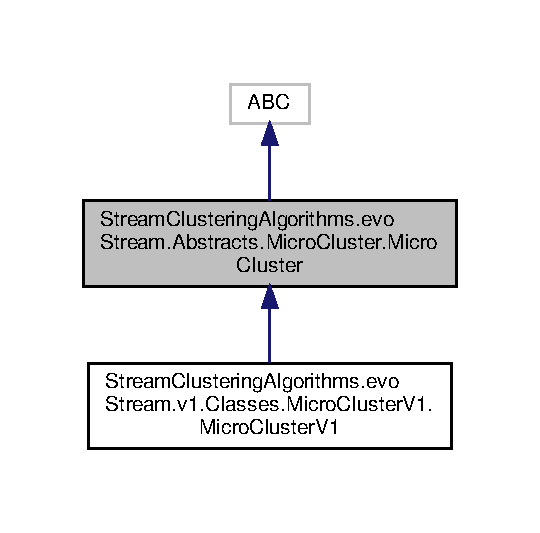
\includegraphics[width=259pt]{classStreamClusteringAlgorithms_1_1evoStream_1_1Abstracts_1_1MicroCluster_1_1MicroCluster__inherit__graph}
\end{center}
\end{figure}


Collaboration diagram for Stream\+Clustering\+Algorithms.\+evo\+Stream.\+Abstracts.\+Micro\+Cluster.\+Micro\+Cluster\+:\nopagebreak
\begin{figure}[H]
\begin{center}
\leavevmode
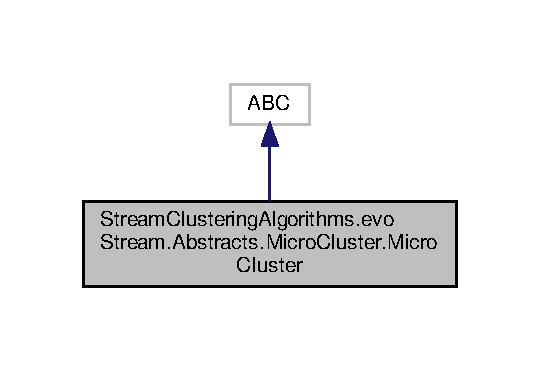
\includegraphics[width=259pt]{classStreamClusteringAlgorithms_1_1evoStream_1_1Abstracts_1_1MicroCluster_1_1MicroCluster__coll__graph}
\end{center}
\end{figure}
\subsection*{Public Member Functions}
\begin{DoxyCompactItemize}
\item 
def \hyperlink{classStreamClusteringAlgorithms_1_1evoStream_1_1Abstracts_1_1MicroCluster_1_1MicroCluster_a3fe909ae28331a372ae182dc210e6b1e}{\+\_\+\+\_\+init\+\_\+\+\_\+} (self, args, kwargs)
\item 
def \hyperlink{classStreamClusteringAlgorithms_1_1evoStream_1_1Abstracts_1_1MicroCluster_1_1MicroCluster_a039c2ba63997e742f0a9947340263745}{jsonify} (self)
\item 
def \hyperlink{classStreamClusteringAlgorithms_1_1evoStream_1_1Abstracts_1_1MicroCluster_1_1MicroCluster_a617f5dcc1bf93101755257ecd364bbcf}{fade} (self, current\+\_\+time, decay\+\_\+rate)
\begin{DoxyCompactList}\small\item\em A base method for aging strategy. \end{DoxyCompactList}\end{DoxyCompactItemize}


\subsection{Detailed Description}
Abstract base class for \hyperlink{classStreamClusteringAlgorithms_1_1evoStream_1_1Abstracts_1_1MicroCluster_1_1MicroCluster}{Micro\+Cluster}. 

\subsection{Constructor \& Destructor Documentation}
\mbox{\Hypertarget{classStreamClusteringAlgorithms_1_1evoStream_1_1Abstracts_1_1MicroCluster_1_1MicroCluster_a3fe909ae28331a372ae182dc210e6b1e}\label{classStreamClusteringAlgorithms_1_1evoStream_1_1Abstracts_1_1MicroCluster_1_1MicroCluster_a3fe909ae28331a372ae182dc210e6b1e}} 
\index{Stream\+Clustering\+Algorithms\+::evo\+Stream\+::\+Abstracts\+::\+Micro\+Cluster\+::\+Micro\+Cluster@{Stream\+Clustering\+Algorithms\+::evo\+Stream\+::\+Abstracts\+::\+Micro\+Cluster\+::\+Micro\+Cluster}!\+\_\+\+\_\+init\+\_\+\+\_\+@{\+\_\+\+\_\+init\+\_\+\+\_\+}}
\index{\+\_\+\+\_\+init\+\_\+\+\_\+@{\+\_\+\+\_\+init\+\_\+\+\_\+}!Stream\+Clustering\+Algorithms\+::evo\+Stream\+::\+Abstracts\+::\+Micro\+Cluster\+::\+Micro\+Cluster@{Stream\+Clustering\+Algorithms\+::evo\+Stream\+::\+Abstracts\+::\+Micro\+Cluster\+::\+Micro\+Cluster}}
\subsubsection{\texorpdfstring{\+\_\+\+\_\+init\+\_\+\+\_\+()}{\_\_init\_\_()}}
{\footnotesize\ttfamily def Stream\+Clustering\+Algorithms.\+evo\+Stream.\+Abstracts.\+Micro\+Cluster.\+Micro\+Cluster.\+\_\+\+\_\+init\+\_\+\+\_\+ (\begin{DoxyParamCaption}\item[{}]{self,  }\item[{}]{args,  }\item[{}]{kwargs }\end{DoxyParamCaption})}



\subsection{Member Function Documentation}
\mbox{\Hypertarget{classStreamClusteringAlgorithms_1_1evoStream_1_1Abstracts_1_1MicroCluster_1_1MicroCluster_a617f5dcc1bf93101755257ecd364bbcf}\label{classStreamClusteringAlgorithms_1_1evoStream_1_1Abstracts_1_1MicroCluster_1_1MicroCluster_a617f5dcc1bf93101755257ecd364bbcf}} 
\index{Stream\+Clustering\+Algorithms\+::evo\+Stream\+::\+Abstracts\+::\+Micro\+Cluster\+::\+Micro\+Cluster@{Stream\+Clustering\+Algorithms\+::evo\+Stream\+::\+Abstracts\+::\+Micro\+Cluster\+::\+Micro\+Cluster}!fade@{fade}}
\index{fade@{fade}!Stream\+Clustering\+Algorithms\+::evo\+Stream\+::\+Abstracts\+::\+Micro\+Cluster\+::\+Micro\+Cluster@{Stream\+Clustering\+Algorithms\+::evo\+Stream\+::\+Abstracts\+::\+Micro\+Cluster\+::\+Micro\+Cluster}}
\subsubsection{\texorpdfstring{fade()}{fade()}}
{\footnotesize\ttfamily def Stream\+Clustering\+Algorithms.\+evo\+Stream.\+Abstracts.\+Micro\+Cluster.\+Micro\+Cluster.\+fade (\begin{DoxyParamCaption}\item[{}]{self,  }\item[{}]{current\+\_\+time,  }\item[{}]{decay\+\_\+rate }\end{DoxyParamCaption})}



A base method for aging strategy. 


\begin{DoxyParams}{Parameters}
{\em current\+\_\+time} & Current Time id  current\+\_\+time\+: int \\
\hline
{\em decay\+\_\+rate} & Decay rate  decay\+\_\+rate\+: float \\
\hline
\end{DoxyParams}
\begin{DoxyReturn}{Returns}
\+: 
\end{DoxyReturn}
\mbox{\Hypertarget{classStreamClusteringAlgorithms_1_1evoStream_1_1Abstracts_1_1MicroCluster_1_1MicroCluster_a039c2ba63997e742f0a9947340263745}\label{classStreamClusteringAlgorithms_1_1evoStream_1_1Abstracts_1_1MicroCluster_1_1MicroCluster_a039c2ba63997e742f0a9947340263745}} 
\index{Stream\+Clustering\+Algorithms\+::evo\+Stream\+::\+Abstracts\+::\+Micro\+Cluster\+::\+Micro\+Cluster@{Stream\+Clustering\+Algorithms\+::evo\+Stream\+::\+Abstracts\+::\+Micro\+Cluster\+::\+Micro\+Cluster}!jsonify@{jsonify}}
\index{jsonify@{jsonify}!Stream\+Clustering\+Algorithms\+::evo\+Stream\+::\+Abstracts\+::\+Micro\+Cluster\+::\+Micro\+Cluster@{Stream\+Clustering\+Algorithms\+::evo\+Stream\+::\+Abstracts\+::\+Micro\+Cluster\+::\+Micro\+Cluster}}
\subsubsection{\texorpdfstring{jsonify()}{jsonify()}}
{\footnotesize\ttfamily def Stream\+Clustering\+Algorithms.\+evo\+Stream.\+Abstracts.\+Micro\+Cluster.\+Micro\+Cluster.\+jsonify (\begin{DoxyParamCaption}\item[{}]{self }\end{DoxyParamCaption})}



The documentation for this class was generated from the following file\+:\begin{DoxyCompactItemize}
\item 
evo\+Stream/\+Abstracts/\hyperlink{MicroCluster_8py}{Micro\+Cluster.\+py}\end{DoxyCompactItemize}

\hypertarget{classStreamClusteringAlgorithms_1_1evoStream_1_1v1_1_1Classes_1_1MicroClusterV1_1_1MicroClusterV1}{}\section{Stream\+Clustering\+Algorithms.\+evo\+Stream.\+v1.\+Classes.\+Micro\+Cluster\+V1.\+Micro\+Cluster\+V1 Class Reference}
\label{classStreamClusteringAlgorithms_1_1evoStream_1_1v1_1_1Classes_1_1MicroClusterV1_1_1MicroClusterV1}\index{Stream\+Clustering\+Algorithms.\+evo\+Stream.\+v1.\+Classes.\+Micro\+Cluster\+V1.\+Micro\+Cluster\+V1@{Stream\+Clustering\+Algorithms.\+evo\+Stream.\+v1.\+Classes.\+Micro\+Cluster\+V1.\+Micro\+Cluster\+V1}}


Inheritance diagram for Stream\+Clustering\+Algorithms.\+evo\+Stream.\+v1.\+Classes.\+Micro\+Cluster\+V1.\+Micro\+Cluster\+V1\+:\nopagebreak
\begin{figure}[H]
\begin{center}
\leavevmode
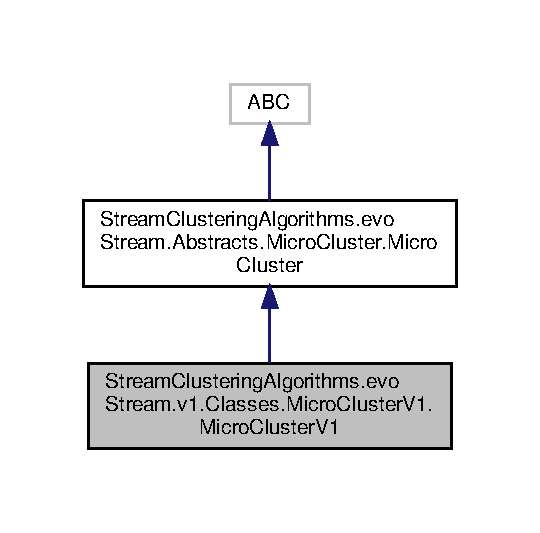
\includegraphics[width=259pt]{classStreamClusteringAlgorithms_1_1evoStream_1_1v1_1_1Classes_1_1MicroClusterV1_1_1MicroClusterV1__inherit__graph}
\end{center}
\end{figure}


Collaboration diagram for Stream\+Clustering\+Algorithms.\+evo\+Stream.\+v1.\+Classes.\+Micro\+Cluster\+V1.\+Micro\+Cluster\+V1\+:\nopagebreak
\begin{figure}[H]
\begin{center}
\leavevmode
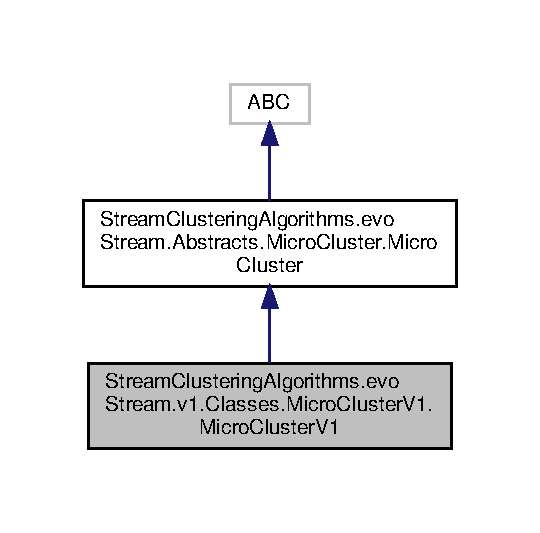
\includegraphics[width=259pt]{classStreamClusteringAlgorithms_1_1evoStream_1_1v1_1_1Classes_1_1MicroClusterV1_1_1MicroClusterV1__coll__graph}
\end{center}
\end{figure}
\subsection*{Public Member Functions}
\begin{DoxyCompactItemize}
\item 
def \hyperlink{classStreamClusteringAlgorithms_1_1evoStream_1_1v1_1_1Classes_1_1MicroClusterV1_1_1MicroClusterV1_a535fe276e2ea722b7526df2b0c7a816d}{\+\_\+\+\_\+init\+\_\+\+\_\+} (self, args, kwargs)
\begin{DoxyCompactList}\small\item\em Constructor of \hyperlink{classStreamClusteringAlgorithms_1_1evoStream_1_1v1_1_1Classes_1_1MicroClusterV1_1_1MicroClusterV1}{Micro\+Cluster\+V1} class. \end{DoxyCompactList}\item 
def \hyperlink{classStreamClusteringAlgorithms_1_1evoStream_1_1v1_1_1Classes_1_1MicroClusterV1_1_1MicroClusterV1_a96848a3f344c55417c2372c96927314c}{jsonify} (self)
\item 
def \hyperlink{classStreamClusteringAlgorithms_1_1evoStream_1_1v1_1_1Classes_1_1MicroClusterV1_1_1MicroClusterV1_ad0bb09e1ba3f158c47ba7712d5c18b72}{fade} (self, current\+\_\+time, decay\+\_\+rate)
\begin{DoxyCompactList}\small\item\em Decay weight according to elapsed time, microcluster is being older. \end{DoxyCompactList}\item 
def \hyperlink{classStreamClusteringAlgorithms_1_1evoStream_1_1v1_1_1Classes_1_1MicroClusterV1_1_1MicroClusterV1_a6eab40d474343e74a914eaa3d341e7d6}{merge} (self, mc, current\+\_\+time, decay\+\_\+rate, radius)
\begin{DoxyCompactList}\small\item\em Absorb new observation by merging centroids according to gaussian neighbourhood coefficient(calc. \end{DoxyCompactList}\item 
def \hyperlink{classStreamClusteringAlgorithms_1_1evoStream_1_1v1_1_1Classes_1_1MicroClusterV1_1_1MicroClusterV1_ad9fd1f97aca72cc3f82e72e2a910932e}{gaussian\+\_\+neighbourhood} (self, \hyperlink{classStreamClusteringAlgorithms_1_1evoStream_1_1v1_1_1Classes_1_1MicroClusterV1_1_1MicroClusterV1_ab8516e0a725a95e796becd032401ddc1}{distance}, radius)
\begin{DoxyCompactList}\small\item\em A method that calculates gaussian neighbourhood coefficient according to distance of two vectors and radius value. \end{DoxyCompactList}\item 
def \hyperlink{classStreamClusteringAlgorithms_1_1evoStream_1_1v1_1_1Classes_1_1MicroClusterV1_1_1MicroClusterV1_ab8516e0a725a95e796becd032401ddc1}{distance} (self, mc)
\begin{DoxyCompactList}\small\item\em Object based distance calculation wrapper, default distance metric is euclidean. \end{DoxyCompactList}\item 
def \hyperlink{classStreamClusteringAlgorithms_1_1evoStream_1_1v1_1_1Classes_1_1MicroClusterV1_1_1MicroClusterV1_aa08f1e1397fba3cf685ab6c57bd618ed}{distance\+\_\+vector} (self, vector)
\begin{DoxyCompactList}\small\item\em Vector based distance calculation wrapper method. \end{DoxyCompactList}\end{DoxyCompactItemize}
\subsection*{Public Attributes}
\begin{DoxyCompactItemize}
\item 
\hyperlink{classStreamClusteringAlgorithms_1_1evoStream_1_1v1_1_1Classes_1_1MicroClusterV1_1_1MicroClusterV1_a1e4653433268a1780f6702c33731645b}{config}
\begin{DoxyCompactList}\small\item\em Class configuration kwargs. \end{DoxyCompactList}\item 
\hyperlink{classStreamClusteringAlgorithms_1_1evoStream_1_1v1_1_1Classes_1_1MicroClusterV1_1_1MicroClusterV1_a1564bd2f57e01b78ba6f32145e2394b3}{centroid}
\begin{DoxyCompactList}\small\item\em Centroid for microcluster initialization. \end{DoxyCompactList}\item 
\hyperlink{classStreamClusteringAlgorithms_1_1evoStream_1_1v1_1_1Classes_1_1MicroClusterV1_1_1MicroClusterV1_a57fcddb96fd19b15fbdb1e6c21d5894c}{last\+\_\+update}
\begin{DoxyCompactList}\small\item\em Weight update formula. \end{DoxyCompactList}\item 
\hyperlink{classStreamClusteringAlgorithms_1_1evoStream_1_1v1_1_1Classes_1_1MicroClusterV1_1_1MicroClusterV1_a41ebafc3c8dd9afa188c2068ceb045ac}{weight}
\item 
\hyperlink{classStreamClusteringAlgorithms_1_1evoStream_1_1v1_1_1Classes_1_1MicroClusterV1_1_1MicroClusterV1_ac09b27bb33c4b34f8006bdf9db081416}{utils}
\begin{DoxyCompactList}\small\item\em Utility interface modules. \end{DoxyCompactList}\end{DoxyCompactItemize}


\subsection{Constructor \& Destructor Documentation}
\mbox{\Hypertarget{classStreamClusteringAlgorithms_1_1evoStream_1_1v1_1_1Classes_1_1MicroClusterV1_1_1MicroClusterV1_a535fe276e2ea722b7526df2b0c7a816d}\label{classStreamClusteringAlgorithms_1_1evoStream_1_1v1_1_1Classes_1_1MicroClusterV1_1_1MicroClusterV1_a535fe276e2ea722b7526df2b0c7a816d}} 
\index{Stream\+Clustering\+Algorithms\+::evo\+Stream\+::v1\+::\+Classes\+::\+Micro\+Cluster\+V1\+::\+Micro\+Cluster\+V1@{Stream\+Clustering\+Algorithms\+::evo\+Stream\+::v1\+::\+Classes\+::\+Micro\+Cluster\+V1\+::\+Micro\+Cluster\+V1}!\+\_\+\+\_\+init\+\_\+\+\_\+@{\+\_\+\+\_\+init\+\_\+\+\_\+}}
\index{\+\_\+\+\_\+init\+\_\+\+\_\+@{\+\_\+\+\_\+init\+\_\+\+\_\+}!Stream\+Clustering\+Algorithms\+::evo\+Stream\+::v1\+::\+Classes\+::\+Micro\+Cluster\+V1\+::\+Micro\+Cluster\+V1@{Stream\+Clustering\+Algorithms\+::evo\+Stream\+::v1\+::\+Classes\+::\+Micro\+Cluster\+V1\+::\+Micro\+Cluster\+V1}}
\subsubsection{\texorpdfstring{\+\_\+\+\_\+init\+\_\+\+\_\+()}{\_\_init\_\_()}}
{\footnotesize\ttfamily def Stream\+Clustering\+Algorithms.\+evo\+Stream.\+v1.\+Classes.\+Micro\+Cluster\+V1.\+Micro\+Cluster\+V1.\+\_\+\+\_\+init\+\_\+\+\_\+ (\begin{DoxyParamCaption}\item[{}]{self,  }\item[{}]{args,  }\item[{}]{kwargs }\end{DoxyParamCaption})}



Constructor of \hyperlink{classStreamClusteringAlgorithms_1_1evoStream_1_1v1_1_1Classes_1_1MicroClusterV1_1_1MicroClusterV1}{Micro\+Cluster\+V1} class. 


\begin{DoxyParams}{Parameters}
{\em args} & \\
\hline
{\em kwargs} & \\
\hline
\end{DoxyParams}


\subsection{Member Function Documentation}
\mbox{\Hypertarget{classStreamClusteringAlgorithms_1_1evoStream_1_1v1_1_1Classes_1_1MicroClusterV1_1_1MicroClusterV1_ab8516e0a725a95e796becd032401ddc1}\label{classStreamClusteringAlgorithms_1_1evoStream_1_1v1_1_1Classes_1_1MicroClusterV1_1_1MicroClusterV1_ab8516e0a725a95e796becd032401ddc1}} 
\index{Stream\+Clustering\+Algorithms\+::evo\+Stream\+::v1\+::\+Classes\+::\+Micro\+Cluster\+V1\+::\+Micro\+Cluster\+V1@{Stream\+Clustering\+Algorithms\+::evo\+Stream\+::v1\+::\+Classes\+::\+Micro\+Cluster\+V1\+::\+Micro\+Cluster\+V1}!distance@{distance}}
\index{distance@{distance}!Stream\+Clustering\+Algorithms\+::evo\+Stream\+::v1\+::\+Classes\+::\+Micro\+Cluster\+V1\+::\+Micro\+Cluster\+V1@{Stream\+Clustering\+Algorithms\+::evo\+Stream\+::v1\+::\+Classes\+::\+Micro\+Cluster\+V1\+::\+Micro\+Cluster\+V1}}
\subsubsection{\texorpdfstring{distance()}{distance()}}
{\footnotesize\ttfamily def Stream\+Clustering\+Algorithms.\+evo\+Stream.\+v1.\+Classes.\+Micro\+Cluster\+V1.\+Micro\+Cluster\+V1.\+distance (\begin{DoxyParamCaption}\item[{}]{self,  }\item[{}]{mc }\end{DoxyParamCaption})}



Object based distance calculation wrapper, default distance metric is euclidean. 


\begin{DoxyParams}{Parameters}
{\em mc} & microcluster object  mc \+: \hyperlink{classStreamClusteringAlgorithms_1_1evoStream_1_1v1_1_1Classes_1_1MicroClusterV1_1_1MicroClusterV1}{Micro\+Cluster\+V1} \\
\hline
\end{DoxyParams}
\begin{DoxyReturn}{Returns}
\+: distance vector  \+: list 
\end{DoxyReturn}
\mbox{\Hypertarget{classStreamClusteringAlgorithms_1_1evoStream_1_1v1_1_1Classes_1_1MicroClusterV1_1_1MicroClusterV1_aa08f1e1397fba3cf685ab6c57bd618ed}\label{classStreamClusteringAlgorithms_1_1evoStream_1_1v1_1_1Classes_1_1MicroClusterV1_1_1MicroClusterV1_aa08f1e1397fba3cf685ab6c57bd618ed}} 
\index{Stream\+Clustering\+Algorithms\+::evo\+Stream\+::v1\+::\+Classes\+::\+Micro\+Cluster\+V1\+::\+Micro\+Cluster\+V1@{Stream\+Clustering\+Algorithms\+::evo\+Stream\+::v1\+::\+Classes\+::\+Micro\+Cluster\+V1\+::\+Micro\+Cluster\+V1}!distance\+\_\+vector@{distance\+\_\+vector}}
\index{distance\+\_\+vector@{distance\+\_\+vector}!Stream\+Clustering\+Algorithms\+::evo\+Stream\+::v1\+::\+Classes\+::\+Micro\+Cluster\+V1\+::\+Micro\+Cluster\+V1@{Stream\+Clustering\+Algorithms\+::evo\+Stream\+::v1\+::\+Classes\+::\+Micro\+Cluster\+V1\+::\+Micro\+Cluster\+V1}}
\subsubsection{\texorpdfstring{distance\+\_\+vector()}{distance\_vector()}}
{\footnotesize\ttfamily def Stream\+Clustering\+Algorithms.\+evo\+Stream.\+v1.\+Classes.\+Micro\+Cluster\+V1.\+Micro\+Cluster\+V1.\+distance\+\_\+vector (\begin{DoxyParamCaption}\item[{}]{self,  }\item[{}]{vector }\end{DoxyParamCaption})}



Vector based distance calculation wrapper method. 


\begin{DoxyParams}{Parameters}
{\em vector} & same sized input vector  vector\+: list \\
\hline
\end{DoxyParams}
\begin{DoxyReturn}{Returns}
\+: distance vector \+: list 
\end{DoxyReturn}
\mbox{\Hypertarget{classStreamClusteringAlgorithms_1_1evoStream_1_1v1_1_1Classes_1_1MicroClusterV1_1_1MicroClusterV1_ad0bb09e1ba3f158c47ba7712d5c18b72}\label{classStreamClusteringAlgorithms_1_1evoStream_1_1v1_1_1Classes_1_1MicroClusterV1_1_1MicroClusterV1_ad0bb09e1ba3f158c47ba7712d5c18b72}} 
\index{Stream\+Clustering\+Algorithms\+::evo\+Stream\+::v1\+::\+Classes\+::\+Micro\+Cluster\+V1\+::\+Micro\+Cluster\+V1@{Stream\+Clustering\+Algorithms\+::evo\+Stream\+::v1\+::\+Classes\+::\+Micro\+Cluster\+V1\+::\+Micro\+Cluster\+V1}!fade@{fade}}
\index{fade@{fade}!Stream\+Clustering\+Algorithms\+::evo\+Stream\+::v1\+::\+Classes\+::\+Micro\+Cluster\+V1\+::\+Micro\+Cluster\+V1@{Stream\+Clustering\+Algorithms\+::evo\+Stream\+::v1\+::\+Classes\+::\+Micro\+Cluster\+V1\+::\+Micro\+Cluster\+V1}}
\subsubsection{\texorpdfstring{fade()}{fade()}}
{\footnotesize\ttfamily def Stream\+Clustering\+Algorithms.\+evo\+Stream.\+v1.\+Classes.\+Micro\+Cluster\+V1.\+Micro\+Cluster\+V1.\+fade (\begin{DoxyParamCaption}\item[{}]{self,  }\item[{}]{current\+\_\+time,  }\item[{}]{decay\+\_\+rate }\end{DoxyParamCaption})}



Decay weight according to elapsed time, microcluster is being older. 


\begin{DoxyParams}{Parameters}
{\em current\+\_\+time} & current time step \\
\hline
{\em decay\+\_\+rate} & weight decay rate \\
\hline
\end{DoxyParams}
\begin{DoxyReturn}{Returns}
\+: 
\end{DoxyReturn}
\mbox{\Hypertarget{classStreamClusteringAlgorithms_1_1evoStream_1_1v1_1_1Classes_1_1MicroClusterV1_1_1MicroClusterV1_ad9fd1f97aca72cc3f82e72e2a910932e}\label{classStreamClusteringAlgorithms_1_1evoStream_1_1v1_1_1Classes_1_1MicroClusterV1_1_1MicroClusterV1_ad9fd1f97aca72cc3f82e72e2a910932e}} 
\index{Stream\+Clustering\+Algorithms\+::evo\+Stream\+::v1\+::\+Classes\+::\+Micro\+Cluster\+V1\+::\+Micro\+Cluster\+V1@{Stream\+Clustering\+Algorithms\+::evo\+Stream\+::v1\+::\+Classes\+::\+Micro\+Cluster\+V1\+::\+Micro\+Cluster\+V1}!gaussian\+\_\+neighbourhood@{gaussian\+\_\+neighbourhood}}
\index{gaussian\+\_\+neighbourhood@{gaussian\+\_\+neighbourhood}!Stream\+Clustering\+Algorithms\+::evo\+Stream\+::v1\+::\+Classes\+::\+Micro\+Cluster\+V1\+::\+Micro\+Cluster\+V1@{Stream\+Clustering\+Algorithms\+::evo\+Stream\+::v1\+::\+Classes\+::\+Micro\+Cluster\+V1\+::\+Micro\+Cluster\+V1}}
\subsubsection{\texorpdfstring{gaussian\+\_\+neighbourhood()}{gaussian\_neighbourhood()}}
{\footnotesize\ttfamily def Stream\+Clustering\+Algorithms.\+evo\+Stream.\+v1.\+Classes.\+Micro\+Cluster\+V1.\+Micro\+Cluster\+V1.\+gaussian\+\_\+neighbourhood (\begin{DoxyParamCaption}\item[{}]{self,  }\item[{}]{distance,  }\item[{}]{radius }\end{DoxyParamCaption})}



A method that calculates gaussian neighbourhood coefficient according to distance of two vectors and radius value. 


\begin{DoxyParams}{Parameters}
{\em distance} & distance between to vectors (default metric is euclidean neighbourhood)  distance\+: float, list \\
\hline
{\em radius} & radius value  radius\+: float \\
\hline
\end{DoxyParams}
\begin{DoxyReturn}{Returns}
\+: gaussian neighbour coefficient \+: float 
\end{DoxyReturn}
\mbox{\Hypertarget{classStreamClusteringAlgorithms_1_1evoStream_1_1v1_1_1Classes_1_1MicroClusterV1_1_1MicroClusterV1_a96848a3f344c55417c2372c96927314c}\label{classStreamClusteringAlgorithms_1_1evoStream_1_1v1_1_1Classes_1_1MicroClusterV1_1_1MicroClusterV1_a96848a3f344c55417c2372c96927314c}} 
\index{Stream\+Clustering\+Algorithms\+::evo\+Stream\+::v1\+::\+Classes\+::\+Micro\+Cluster\+V1\+::\+Micro\+Cluster\+V1@{Stream\+Clustering\+Algorithms\+::evo\+Stream\+::v1\+::\+Classes\+::\+Micro\+Cluster\+V1\+::\+Micro\+Cluster\+V1}!jsonify@{jsonify}}
\index{jsonify@{jsonify}!Stream\+Clustering\+Algorithms\+::evo\+Stream\+::v1\+::\+Classes\+::\+Micro\+Cluster\+V1\+::\+Micro\+Cluster\+V1@{Stream\+Clustering\+Algorithms\+::evo\+Stream\+::v1\+::\+Classes\+::\+Micro\+Cluster\+V1\+::\+Micro\+Cluster\+V1}}
\subsubsection{\texorpdfstring{jsonify()}{jsonify()}}
{\footnotesize\ttfamily def Stream\+Clustering\+Algorithms.\+evo\+Stream.\+v1.\+Classes.\+Micro\+Cluster\+V1.\+Micro\+Cluster\+V1.\+jsonify (\begin{DoxyParamCaption}\item[{}]{self }\end{DoxyParamCaption})}

\mbox{\Hypertarget{classStreamClusteringAlgorithms_1_1evoStream_1_1v1_1_1Classes_1_1MicroClusterV1_1_1MicroClusterV1_a6eab40d474343e74a914eaa3d341e7d6}\label{classStreamClusteringAlgorithms_1_1evoStream_1_1v1_1_1Classes_1_1MicroClusterV1_1_1MicroClusterV1_a6eab40d474343e74a914eaa3d341e7d6}} 
\index{Stream\+Clustering\+Algorithms\+::evo\+Stream\+::v1\+::\+Classes\+::\+Micro\+Cluster\+V1\+::\+Micro\+Cluster\+V1@{Stream\+Clustering\+Algorithms\+::evo\+Stream\+::v1\+::\+Classes\+::\+Micro\+Cluster\+V1\+::\+Micro\+Cluster\+V1}!merge@{merge}}
\index{merge@{merge}!Stream\+Clustering\+Algorithms\+::evo\+Stream\+::v1\+::\+Classes\+::\+Micro\+Cluster\+V1\+::\+Micro\+Cluster\+V1@{Stream\+Clustering\+Algorithms\+::evo\+Stream\+::v1\+::\+Classes\+::\+Micro\+Cluster\+V1\+::\+Micro\+Cluster\+V1}}
\subsubsection{\texorpdfstring{merge()}{merge()}}
{\footnotesize\ttfamily def Stream\+Clustering\+Algorithms.\+evo\+Stream.\+v1.\+Classes.\+Micro\+Cluster\+V1.\+Micro\+Cluster\+V1.\+merge (\begin{DoxyParamCaption}\item[{}]{self,  }\item[{}]{mc,  }\item[{}]{current\+\_\+time,  }\item[{}]{decay\+\_\+rate,  }\item[{}]{radius }\end{DoxyParamCaption})}



Absorb new observation by merging centroids according to gaussian neighbourhood coefficient(calc. 

acc. to radius and distance) 
\begin{DoxyParams}{Parameters}
{\em mc} & microcluster object \\
\hline
{\em current\+\_\+time} & current time step \\
\hline
{\em decay\+\_\+rate} & weight decay rate \\
\hline
{\em radius} & \\
\hline
\end{DoxyParams}
\begin{DoxyReturn}{Returns}
\+: None, Updated microcluster centroids as inplace 
\end{DoxyReturn}


\subsection{Member Data Documentation}
\mbox{\Hypertarget{classStreamClusteringAlgorithms_1_1evoStream_1_1v1_1_1Classes_1_1MicroClusterV1_1_1MicroClusterV1_a1564bd2f57e01b78ba6f32145e2394b3}\label{classStreamClusteringAlgorithms_1_1evoStream_1_1v1_1_1Classes_1_1MicroClusterV1_1_1MicroClusterV1_a1564bd2f57e01b78ba6f32145e2394b3}} 
\index{Stream\+Clustering\+Algorithms\+::evo\+Stream\+::v1\+::\+Classes\+::\+Micro\+Cluster\+V1\+::\+Micro\+Cluster\+V1@{Stream\+Clustering\+Algorithms\+::evo\+Stream\+::v1\+::\+Classes\+::\+Micro\+Cluster\+V1\+::\+Micro\+Cluster\+V1}!centroid@{centroid}}
\index{centroid@{centroid}!Stream\+Clustering\+Algorithms\+::evo\+Stream\+::v1\+::\+Classes\+::\+Micro\+Cluster\+V1\+::\+Micro\+Cluster\+V1@{Stream\+Clustering\+Algorithms\+::evo\+Stream\+::v1\+::\+Classes\+::\+Micro\+Cluster\+V1\+::\+Micro\+Cluster\+V1}}
\subsubsection{\texorpdfstring{centroid}{centroid}}
{\footnotesize\ttfamily Stream\+Clustering\+Algorithms.\+evo\+Stream.\+v1.\+Classes.\+Micro\+Cluster\+V1.\+Micro\+Cluster\+V1.\+centroid}



Centroid for microcluster initialization. 

\mbox{\Hypertarget{classStreamClusteringAlgorithms_1_1evoStream_1_1v1_1_1Classes_1_1MicroClusterV1_1_1MicroClusterV1_a1e4653433268a1780f6702c33731645b}\label{classStreamClusteringAlgorithms_1_1evoStream_1_1v1_1_1Classes_1_1MicroClusterV1_1_1MicroClusterV1_a1e4653433268a1780f6702c33731645b}} 
\index{Stream\+Clustering\+Algorithms\+::evo\+Stream\+::v1\+::\+Classes\+::\+Micro\+Cluster\+V1\+::\+Micro\+Cluster\+V1@{Stream\+Clustering\+Algorithms\+::evo\+Stream\+::v1\+::\+Classes\+::\+Micro\+Cluster\+V1\+::\+Micro\+Cluster\+V1}!config@{config}}
\index{config@{config}!Stream\+Clustering\+Algorithms\+::evo\+Stream\+::v1\+::\+Classes\+::\+Micro\+Cluster\+V1\+::\+Micro\+Cluster\+V1@{Stream\+Clustering\+Algorithms\+::evo\+Stream\+::v1\+::\+Classes\+::\+Micro\+Cluster\+V1\+::\+Micro\+Cluster\+V1}}
\subsubsection{\texorpdfstring{config}{config}}
{\footnotesize\ttfamily Stream\+Clustering\+Algorithms.\+evo\+Stream.\+v1.\+Classes.\+Micro\+Cluster\+V1.\+Micro\+Cluster\+V1.\+config}



Class configuration kwargs. 

\mbox{\Hypertarget{classStreamClusteringAlgorithms_1_1evoStream_1_1v1_1_1Classes_1_1MicroClusterV1_1_1MicroClusterV1_a57fcddb96fd19b15fbdb1e6c21d5894c}\label{classStreamClusteringAlgorithms_1_1evoStream_1_1v1_1_1Classes_1_1MicroClusterV1_1_1MicroClusterV1_a57fcddb96fd19b15fbdb1e6c21d5894c}} 
\index{Stream\+Clustering\+Algorithms\+::evo\+Stream\+::v1\+::\+Classes\+::\+Micro\+Cluster\+V1\+::\+Micro\+Cluster\+V1@{Stream\+Clustering\+Algorithms\+::evo\+Stream\+::v1\+::\+Classes\+::\+Micro\+Cluster\+V1\+::\+Micro\+Cluster\+V1}!last\+\_\+update@{last\+\_\+update}}
\index{last\+\_\+update@{last\+\_\+update}!Stream\+Clustering\+Algorithms\+::evo\+Stream\+::v1\+::\+Classes\+::\+Micro\+Cluster\+V1\+::\+Micro\+Cluster\+V1@{Stream\+Clustering\+Algorithms\+::evo\+Stream\+::v1\+::\+Classes\+::\+Micro\+Cluster\+V1\+::\+Micro\+Cluster\+V1}}
\subsubsection{\texorpdfstring{last\+\_\+update}{last\_update}}
{\footnotesize\ttfamily Stream\+Clustering\+Algorithms.\+evo\+Stream.\+v1.\+Classes.\+Micro\+Cluster\+V1.\+Micro\+Cluster\+V1.\+last\+\_\+update}



Weight update formula. 

Time update \mbox{\Hypertarget{classStreamClusteringAlgorithms_1_1evoStream_1_1v1_1_1Classes_1_1MicroClusterV1_1_1MicroClusterV1_ac09b27bb33c4b34f8006bdf9db081416}\label{classStreamClusteringAlgorithms_1_1evoStream_1_1v1_1_1Classes_1_1MicroClusterV1_1_1MicroClusterV1_ac09b27bb33c4b34f8006bdf9db081416}} 
\index{Stream\+Clustering\+Algorithms\+::evo\+Stream\+::v1\+::\+Classes\+::\+Micro\+Cluster\+V1\+::\+Micro\+Cluster\+V1@{Stream\+Clustering\+Algorithms\+::evo\+Stream\+::v1\+::\+Classes\+::\+Micro\+Cluster\+V1\+::\+Micro\+Cluster\+V1}!utils@{utils}}
\index{utils@{utils}!Stream\+Clustering\+Algorithms\+::evo\+Stream\+::v1\+::\+Classes\+::\+Micro\+Cluster\+V1\+::\+Micro\+Cluster\+V1@{Stream\+Clustering\+Algorithms\+::evo\+Stream\+::v1\+::\+Classes\+::\+Micro\+Cluster\+V1\+::\+Micro\+Cluster\+V1}}
\subsubsection{\texorpdfstring{utils}{utils}}
{\footnotesize\ttfamily Stream\+Clustering\+Algorithms.\+evo\+Stream.\+v1.\+Classes.\+Micro\+Cluster\+V1.\+Micro\+Cluster\+V1.\+utils}



Utility interface modules. 

\mbox{\Hypertarget{classStreamClusteringAlgorithms_1_1evoStream_1_1v1_1_1Classes_1_1MicroClusterV1_1_1MicroClusterV1_a41ebafc3c8dd9afa188c2068ceb045ac}\label{classStreamClusteringAlgorithms_1_1evoStream_1_1v1_1_1Classes_1_1MicroClusterV1_1_1MicroClusterV1_a41ebafc3c8dd9afa188c2068ceb045ac}} 
\index{Stream\+Clustering\+Algorithms\+::evo\+Stream\+::v1\+::\+Classes\+::\+Micro\+Cluster\+V1\+::\+Micro\+Cluster\+V1@{Stream\+Clustering\+Algorithms\+::evo\+Stream\+::v1\+::\+Classes\+::\+Micro\+Cluster\+V1\+::\+Micro\+Cluster\+V1}!weight@{weight}}
\index{weight@{weight}!Stream\+Clustering\+Algorithms\+::evo\+Stream\+::v1\+::\+Classes\+::\+Micro\+Cluster\+V1\+::\+Micro\+Cluster\+V1@{Stream\+Clustering\+Algorithms\+::evo\+Stream\+::v1\+::\+Classes\+::\+Micro\+Cluster\+V1\+::\+Micro\+Cluster\+V1}}
\subsubsection{\texorpdfstring{weight}{weight}}
{\footnotesize\ttfamily Stream\+Clustering\+Algorithms.\+evo\+Stream.\+v1.\+Classes.\+Micro\+Cluster\+V1.\+Micro\+Cluster\+V1.\+weight}



The documentation for this class was generated from the following file\+:\begin{DoxyCompactItemize}
\item 
evo\+Stream/v1/\+Classes/\hyperlink{MicroClusterV1_8py}{Micro\+Cluster\+V1.\+py}\end{DoxyCompactItemize}

\hypertarget{classStreamClusteringAlgorithms_1_1evoStream_1_1v1_1_1Tests_1_1EvoStreamv1Test_1_1Test}{}\section{Stream\+Clustering\+Algorithms.\+evo\+Stream.\+v1.\+Tests.\+Evo\+Streamv1\+Test.\+Test Class Reference}
\label{classStreamClusteringAlgorithms_1_1evoStream_1_1v1_1_1Tests_1_1EvoStreamv1Test_1_1Test}\index{Stream\+Clustering\+Algorithms.\+evo\+Stream.\+v1.\+Tests.\+Evo\+Streamv1\+Test.\+Test@{Stream\+Clustering\+Algorithms.\+evo\+Stream.\+v1.\+Tests.\+Evo\+Streamv1\+Test.\+Test}}


Inheritance diagram for Stream\+Clustering\+Algorithms.\+evo\+Stream.\+v1.\+Tests.\+Evo\+Streamv1\+Test.\+Test\+:\nopagebreak
\begin{figure}[H]
\begin{center}
\leavevmode
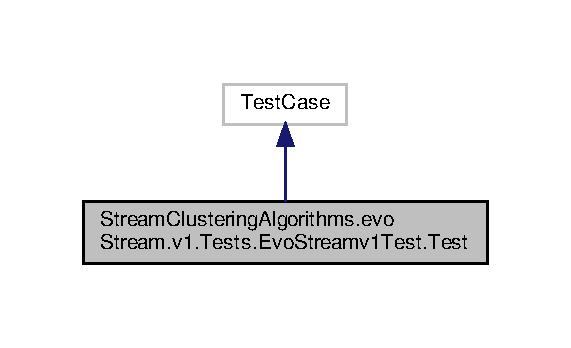
\includegraphics[width=274pt]{classStreamClusteringAlgorithms_1_1evoStream_1_1v1_1_1Tests_1_1EvoStreamv1Test_1_1Test__inherit__graph}
\end{center}
\end{figure}


Collaboration diagram for Stream\+Clustering\+Algorithms.\+evo\+Stream.\+v1.\+Tests.\+Evo\+Streamv1\+Test.\+Test\+:\nopagebreak
\begin{figure}[H]
\begin{center}
\leavevmode
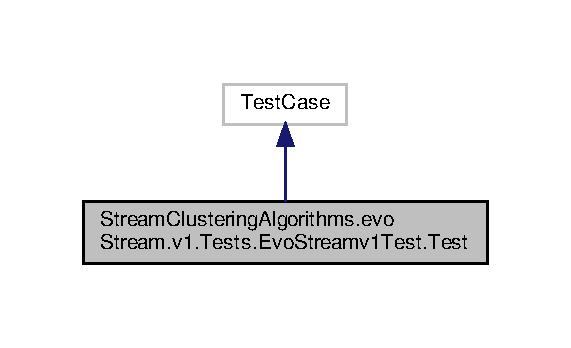
\includegraphics[width=274pt]{classStreamClusteringAlgorithms_1_1evoStream_1_1v1_1_1Tests_1_1EvoStreamv1Test_1_1Test__coll__graph}
\end{center}
\end{figure}
\subsection*{Public Member Functions}
\begin{DoxyCompactItemize}
\item 
def \hyperlink{classStreamClusteringAlgorithms_1_1evoStream_1_1v1_1_1Tests_1_1EvoStreamv1Test_1_1Test_a417ff4abae3adcea11c96540b55cebaa}{set\+Up} (self)
\begin{DoxyCompactList}\small\item\em Setting up algorithm object and observations for test methods. \end{DoxyCompactList}\item 
def \hyperlink{classStreamClusteringAlgorithms_1_1evoStream_1_1v1_1_1Tests_1_1EvoStreamv1Test_1_1Test_a6687b34b5280ecf25865914f7e5b4b35}{tear\+Down} (self)
\item 
def \hyperlink{classStreamClusteringAlgorithms_1_1evoStream_1_1v1_1_1Tests_1_1EvoStreamv1Test_1_1Test_a083882949698c86a856604a5467d0e35}{test\+\_\+pipeline} (self)
\begin{DoxyCompactList}\small\item\em Pipeline test of clustering mechanism. \end{DoxyCompactList}\item 
def \hyperlink{classStreamClusteringAlgorithms_1_1evoStream_1_1v1_1_1Tests_1_1EvoStreamv1Test_1_1Test_a1e1c9b48bef84a01ede43b88e1a9103a}{test\+\_\+predictions} (self)
\begin{DoxyCompactList}\small\item\em \hyperlink{classStreamClusteringAlgorithms_1_1evoStream_1_1v1_1_1Tests_1_1EvoStreamv1Test_1_1Test}{Test} of algorithm predictions. \end{DoxyCompactList}\end{DoxyCompactItemize}
\subsection*{Public Attributes}
\begin{DoxyCompactItemize}
\item 
\hyperlink{classStreamClusteringAlgorithms_1_1evoStream_1_1v1_1_1Tests_1_1EvoStreamv1Test_1_1Test_a9db3219943754c41bcab6ed2bb8f8b9b}{evo}
\item 
\hyperlink{classStreamClusteringAlgorithms_1_1evoStream_1_1v1_1_1Tests_1_1EvoStreamv1Test_1_1Test_a4c28200e5e876b8fde116193e71c443b}{observation}
\end{DoxyCompactItemize}


\subsection{Member Function Documentation}
\mbox{\Hypertarget{classStreamClusteringAlgorithms_1_1evoStream_1_1v1_1_1Tests_1_1EvoStreamv1Test_1_1Test_a417ff4abae3adcea11c96540b55cebaa}\label{classStreamClusteringAlgorithms_1_1evoStream_1_1v1_1_1Tests_1_1EvoStreamv1Test_1_1Test_a417ff4abae3adcea11c96540b55cebaa}} 
\index{Stream\+Clustering\+Algorithms\+::evo\+Stream\+::v1\+::\+Tests\+::\+Evo\+Streamv1\+Test\+::\+Test@{Stream\+Clustering\+Algorithms\+::evo\+Stream\+::v1\+::\+Tests\+::\+Evo\+Streamv1\+Test\+::\+Test}!set\+Up@{set\+Up}}
\index{set\+Up@{set\+Up}!Stream\+Clustering\+Algorithms\+::evo\+Stream\+::v1\+::\+Tests\+::\+Evo\+Streamv1\+Test\+::\+Test@{Stream\+Clustering\+Algorithms\+::evo\+Stream\+::v1\+::\+Tests\+::\+Evo\+Streamv1\+Test\+::\+Test}}
\subsubsection{\texorpdfstring{set\+Up()}{setUp()}}
{\footnotesize\ttfamily def Stream\+Clustering\+Algorithms.\+evo\+Stream.\+v1.\+Tests.\+Evo\+Streamv1\+Test.\+Test.\+set\+Up (\begin{DoxyParamCaption}\item[{}]{self,  }\item[{}]{None }\end{DoxyParamCaption})}



Setting up algorithm object and observations for test methods. 

\begin{DoxyReturn}{Returns}
\+: 
\end{DoxyReturn}
\mbox{\Hypertarget{classStreamClusteringAlgorithms_1_1evoStream_1_1v1_1_1Tests_1_1EvoStreamv1Test_1_1Test_a6687b34b5280ecf25865914f7e5b4b35}\label{classStreamClusteringAlgorithms_1_1evoStream_1_1v1_1_1Tests_1_1EvoStreamv1Test_1_1Test_a6687b34b5280ecf25865914f7e5b4b35}} 
\index{Stream\+Clustering\+Algorithms\+::evo\+Stream\+::v1\+::\+Tests\+::\+Evo\+Streamv1\+Test\+::\+Test@{Stream\+Clustering\+Algorithms\+::evo\+Stream\+::v1\+::\+Tests\+::\+Evo\+Streamv1\+Test\+::\+Test}!tear\+Down@{tear\+Down}}
\index{tear\+Down@{tear\+Down}!Stream\+Clustering\+Algorithms\+::evo\+Stream\+::v1\+::\+Tests\+::\+Evo\+Streamv1\+Test\+::\+Test@{Stream\+Clustering\+Algorithms\+::evo\+Stream\+::v1\+::\+Tests\+::\+Evo\+Streamv1\+Test\+::\+Test}}
\subsubsection{\texorpdfstring{tear\+Down()}{tearDown()}}
{\footnotesize\ttfamily def Stream\+Clustering\+Algorithms.\+evo\+Stream.\+v1.\+Tests.\+Evo\+Streamv1\+Test.\+Test.\+tear\+Down (\begin{DoxyParamCaption}\item[{}]{self,  }\item[{}]{None }\end{DoxyParamCaption})}

\mbox{\Hypertarget{classStreamClusteringAlgorithms_1_1evoStream_1_1v1_1_1Tests_1_1EvoStreamv1Test_1_1Test_a083882949698c86a856604a5467d0e35}\label{classStreamClusteringAlgorithms_1_1evoStream_1_1v1_1_1Tests_1_1EvoStreamv1Test_1_1Test_a083882949698c86a856604a5467d0e35}} 
\index{Stream\+Clustering\+Algorithms\+::evo\+Stream\+::v1\+::\+Tests\+::\+Evo\+Streamv1\+Test\+::\+Test@{Stream\+Clustering\+Algorithms\+::evo\+Stream\+::v1\+::\+Tests\+::\+Evo\+Streamv1\+Test\+::\+Test}!test\+\_\+pipeline@{test\+\_\+pipeline}}
\index{test\+\_\+pipeline@{test\+\_\+pipeline}!Stream\+Clustering\+Algorithms\+::evo\+Stream\+::v1\+::\+Tests\+::\+Evo\+Streamv1\+Test\+::\+Test@{Stream\+Clustering\+Algorithms\+::evo\+Stream\+::v1\+::\+Tests\+::\+Evo\+Streamv1\+Test\+::\+Test}}
\subsubsection{\texorpdfstring{test\+\_\+pipeline()}{test\_pipeline()}}
{\footnotesize\ttfamily def Stream\+Clustering\+Algorithms.\+evo\+Stream.\+v1.\+Tests.\+Evo\+Streamv1\+Test.\+Test.\+test\+\_\+pipeline (\begin{DoxyParamCaption}\item[{}]{self }\end{DoxyParamCaption})}



Pipeline test of clustering mechanism. 

\begin{DoxyReturn}{Returns}
\+: 
\end{DoxyReturn}
\mbox{\Hypertarget{classStreamClusteringAlgorithms_1_1evoStream_1_1v1_1_1Tests_1_1EvoStreamv1Test_1_1Test_a1e1c9b48bef84a01ede43b88e1a9103a}\label{classStreamClusteringAlgorithms_1_1evoStream_1_1v1_1_1Tests_1_1EvoStreamv1Test_1_1Test_a1e1c9b48bef84a01ede43b88e1a9103a}} 
\index{Stream\+Clustering\+Algorithms\+::evo\+Stream\+::v1\+::\+Tests\+::\+Evo\+Streamv1\+Test\+::\+Test@{Stream\+Clustering\+Algorithms\+::evo\+Stream\+::v1\+::\+Tests\+::\+Evo\+Streamv1\+Test\+::\+Test}!test\+\_\+predictions@{test\+\_\+predictions}}
\index{test\+\_\+predictions@{test\+\_\+predictions}!Stream\+Clustering\+Algorithms\+::evo\+Stream\+::v1\+::\+Tests\+::\+Evo\+Streamv1\+Test\+::\+Test@{Stream\+Clustering\+Algorithms\+::evo\+Stream\+::v1\+::\+Tests\+::\+Evo\+Streamv1\+Test\+::\+Test}}
\subsubsection{\texorpdfstring{test\+\_\+predictions()}{test\_predictions()}}
{\footnotesize\ttfamily def Stream\+Clustering\+Algorithms.\+evo\+Stream.\+v1.\+Tests.\+Evo\+Streamv1\+Test.\+Test.\+test\+\_\+predictions (\begin{DoxyParamCaption}\item[{}]{self }\end{DoxyParamCaption})}



\hyperlink{classStreamClusteringAlgorithms_1_1evoStream_1_1v1_1_1Tests_1_1EvoStreamv1Test_1_1Test}{Test} of algorithm predictions. 

If the colored dots in the scatter plot are seperated. Primitive PoC is done. \begin{DoxyReturn}{Returns}
\+: 
\end{DoxyReturn}


\subsection{Member Data Documentation}
\mbox{\Hypertarget{classStreamClusteringAlgorithms_1_1evoStream_1_1v1_1_1Tests_1_1EvoStreamv1Test_1_1Test_a9db3219943754c41bcab6ed2bb8f8b9b}\label{classStreamClusteringAlgorithms_1_1evoStream_1_1v1_1_1Tests_1_1EvoStreamv1Test_1_1Test_a9db3219943754c41bcab6ed2bb8f8b9b}} 
\index{Stream\+Clustering\+Algorithms\+::evo\+Stream\+::v1\+::\+Tests\+::\+Evo\+Streamv1\+Test\+::\+Test@{Stream\+Clustering\+Algorithms\+::evo\+Stream\+::v1\+::\+Tests\+::\+Evo\+Streamv1\+Test\+::\+Test}!evo@{evo}}
\index{evo@{evo}!Stream\+Clustering\+Algorithms\+::evo\+Stream\+::v1\+::\+Tests\+::\+Evo\+Streamv1\+Test\+::\+Test@{Stream\+Clustering\+Algorithms\+::evo\+Stream\+::v1\+::\+Tests\+::\+Evo\+Streamv1\+Test\+::\+Test}}
\subsubsection{\texorpdfstring{evo}{evo}}
{\footnotesize\ttfamily Stream\+Clustering\+Algorithms.\+evo\+Stream.\+v1.\+Tests.\+Evo\+Streamv1\+Test.\+Test.\+evo}

\mbox{\Hypertarget{classStreamClusteringAlgorithms_1_1evoStream_1_1v1_1_1Tests_1_1EvoStreamv1Test_1_1Test_a4c28200e5e876b8fde116193e71c443b}\label{classStreamClusteringAlgorithms_1_1evoStream_1_1v1_1_1Tests_1_1EvoStreamv1Test_1_1Test_a4c28200e5e876b8fde116193e71c443b}} 
\index{Stream\+Clustering\+Algorithms\+::evo\+Stream\+::v1\+::\+Tests\+::\+Evo\+Streamv1\+Test\+::\+Test@{Stream\+Clustering\+Algorithms\+::evo\+Stream\+::v1\+::\+Tests\+::\+Evo\+Streamv1\+Test\+::\+Test}!observation@{observation}}
\index{observation@{observation}!Stream\+Clustering\+Algorithms\+::evo\+Stream\+::v1\+::\+Tests\+::\+Evo\+Streamv1\+Test\+::\+Test@{Stream\+Clustering\+Algorithms\+::evo\+Stream\+::v1\+::\+Tests\+::\+Evo\+Streamv1\+Test\+::\+Test}}
\subsubsection{\texorpdfstring{observation}{observation}}
{\footnotesize\ttfamily Stream\+Clustering\+Algorithms.\+evo\+Stream.\+v1.\+Tests.\+Evo\+Streamv1\+Test.\+Test.\+observation}



The documentation for this class was generated from the following file\+:\begin{DoxyCompactItemize}
\item 
evo\+Stream/v1/\+Tests/\hyperlink{EvoStreamv1Test_8py}{Evo\+Streamv1\+Test.\+py}\end{DoxyCompactItemize}

\hypertarget{classStreamClusteringAlgorithms_1_1evoStream_1_1v1_1_1Tests_1_1MicroClusterV1Test_1_1Test}{}\section{Stream\+Clustering\+Algorithms.\+evo\+Stream.\+v1.\+Tests.\+Micro\+Cluster\+V1\+Test.\+Test Class Reference}
\label{classStreamClusteringAlgorithms_1_1evoStream_1_1v1_1_1Tests_1_1MicroClusterV1Test_1_1Test}\index{Stream\+Clustering\+Algorithms.\+evo\+Stream.\+v1.\+Tests.\+Micro\+Cluster\+V1\+Test.\+Test@{Stream\+Clustering\+Algorithms.\+evo\+Stream.\+v1.\+Tests.\+Micro\+Cluster\+V1\+Test.\+Test}}


Inheritance diagram for Stream\+Clustering\+Algorithms.\+evo\+Stream.\+v1.\+Tests.\+Micro\+Cluster\+V1\+Test.\+Test\+:\nopagebreak
\begin{figure}[H]
\begin{center}
\leavevmode
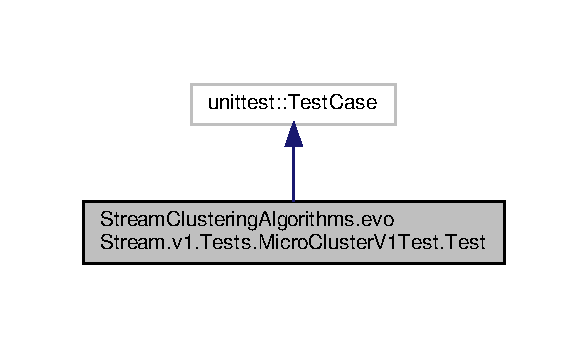
\includegraphics[width=282pt]{classStreamClusteringAlgorithms_1_1evoStream_1_1v1_1_1Tests_1_1MicroClusterV1Test_1_1Test__inherit__graph}
\end{center}
\end{figure}


Collaboration diagram for Stream\+Clustering\+Algorithms.\+evo\+Stream.\+v1.\+Tests.\+Micro\+Cluster\+V1\+Test.\+Test\+:\nopagebreak
\begin{figure}[H]
\begin{center}
\leavevmode
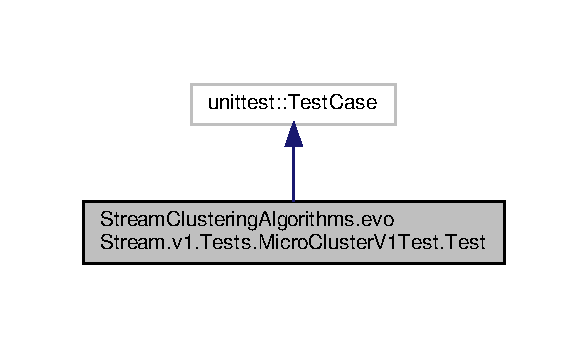
\includegraphics[width=282pt]{classStreamClusteringAlgorithms_1_1evoStream_1_1v1_1_1Tests_1_1MicroClusterV1Test_1_1Test__coll__graph}
\end{center}
\end{figure}
\subsection*{Public Member Functions}
\begin{DoxyCompactItemize}
\item 
def \hyperlink{classStreamClusteringAlgorithms_1_1evoStream_1_1v1_1_1Tests_1_1MicroClusterV1Test_1_1Test_a3061a186eb72fa52eff8851954b2639b}{set\+Up} (self)
\begin{DoxyCompactList}\small\item\em Microcluster object initialization for test methods. \end{DoxyCompactList}\item 
def \hyperlink{classStreamClusteringAlgorithms_1_1evoStream_1_1v1_1_1Tests_1_1MicroClusterV1Test_1_1Test_af251f92c9394f8b8c06b834871653653}{tear\+Down} (self)
\item 
def \hyperlink{classStreamClusteringAlgorithms_1_1evoStream_1_1v1_1_1Tests_1_1MicroClusterV1Test_1_1Test_ac39ed972c17ae27514d264fbe2a73b73}{test\+\_\+microcluster\+\_\+initialization} (self)
\begin{DoxyCompactList}\small\item\em \hyperlink{classStreamClusteringAlgorithms_1_1evoStream_1_1v1_1_1Tests_1_1MicroClusterV1Test_1_1Test}{Test} for microcluster initialization. \end{DoxyCompactList}\item 
def \hyperlink{classStreamClusteringAlgorithms_1_1evoStream_1_1v1_1_1Tests_1_1MicroClusterV1Test_1_1Test_a2adb5543257fd5ad77b753dd8710edaf}{test\+\_\+microcluster\+\_\+vector\+\_\+distance} (self)
\begin{DoxyCompactList}\small\item\em \hyperlink{classStreamClusteringAlgorithms_1_1evoStream_1_1v1_1_1Tests_1_1MicroClusterV1Test_1_1Test}{Test} for microcluster vector distance. \end{DoxyCompactList}\item 
def \hyperlink{classStreamClusteringAlgorithms_1_1evoStream_1_1v1_1_1Tests_1_1MicroClusterV1Test_1_1Test_a3faffdf61680aa04887298598929d6e4}{test\+\_\+microcluster\+\_\+object\+\_\+distance} (self)
\begin{DoxyCompactList}\small\item\em \hyperlink{classStreamClusteringAlgorithms_1_1evoStream_1_1v1_1_1Tests_1_1MicroClusterV1Test_1_1Test}{Test} for microcluster object distance. \end{DoxyCompactList}\item 
def \hyperlink{classStreamClusteringAlgorithms_1_1evoStream_1_1v1_1_1Tests_1_1MicroClusterV1Test_1_1Test_a0d79eac574b5292c7901cbf4ed640ca3}{test\+\_\+microcluster\+\_\+gaussian\+\_\+neighbourhood} (self)
\begin{DoxyCompactList}\small\item\em \hyperlink{classStreamClusteringAlgorithms_1_1evoStream_1_1v1_1_1Tests_1_1MicroClusterV1Test_1_1Test}{Test} for gaussian neighbourhood. \end{DoxyCompactList}\item 
def \hyperlink{classStreamClusteringAlgorithms_1_1evoStream_1_1v1_1_1Tests_1_1MicroClusterV1Test_1_1Test_ad4b4beb7a4f40cdfffa8c2f88c4778f5}{test\+\_\+microcluster\+\_\+fade} (self)
\begin{DoxyCompactList}\small\item\em \hyperlink{classStreamClusteringAlgorithms_1_1evoStream_1_1v1_1_1Tests_1_1MicroClusterV1Test_1_1Test}{Test} for fading microcluster. \end{DoxyCompactList}\item 
def \hyperlink{classStreamClusteringAlgorithms_1_1evoStream_1_1v1_1_1Tests_1_1MicroClusterV1Test_1_1Test_ad83330697fbcbd11b5aa21f8433fd769}{test\+\_\+microcluster\+\_\+same\+\_\+fade} (self)
\begin{DoxyCompactList}\small\item\em \hyperlink{classStreamClusteringAlgorithms_1_1evoStream_1_1v1_1_1Tests_1_1MicroClusterV1Test_1_1Test}{Test} for fading microcluster. \end{DoxyCompactList}\item 
def \hyperlink{classStreamClusteringAlgorithms_1_1evoStream_1_1v1_1_1Tests_1_1MicroClusterV1Test_1_1Test_aebd05484219193bbe05176e04964b7e8}{test\+\_\+microcluster\+\_\+merge} (self)
\begin{DoxyCompactList}\small\item\em \hyperlink{classStreamClusteringAlgorithms_1_1evoStream_1_1v1_1_1Tests_1_1MicroClusterV1Test_1_1Test}{Test} for merge microclusters. \end{DoxyCompactList}\end{DoxyCompactItemize}
\subsection*{Public Attributes}
\begin{DoxyCompactItemize}
\item 
\hyperlink{classStreamClusteringAlgorithms_1_1evoStream_1_1v1_1_1Tests_1_1MicroClusterV1Test_1_1Test_a85e023986389b8720b08b9c8103caa2a}{mc}
\item 
\hyperlink{classStreamClusteringAlgorithms_1_1evoStream_1_1v1_1_1Tests_1_1MicroClusterV1Test_1_1Test_a4cc0f32d424cd9fa7d24c89a094b5beb}{mc2}
\item 
\hyperlink{classStreamClusteringAlgorithms_1_1evoStream_1_1v1_1_1Tests_1_1MicroClusterV1Test_1_1Test_ac88ace2bf500b5b16bc4b52b5aea2caf}{radius}
\item 
\hyperlink{classStreamClusteringAlgorithms_1_1evoStream_1_1v1_1_1Tests_1_1MicroClusterV1Test_1_1Test_ada8a8303e891139420558721368d3d9f}{current\+\_\+time}
\item 
\hyperlink{classStreamClusteringAlgorithms_1_1evoStream_1_1v1_1_1Tests_1_1MicroClusterV1Test_1_1Test_a0208121554a10abdad3cb101491efda3}{decay\+\_\+rate}
\end{DoxyCompactItemize}


\subsection{Member Function Documentation}
\mbox{\Hypertarget{classStreamClusteringAlgorithms_1_1evoStream_1_1v1_1_1Tests_1_1MicroClusterV1Test_1_1Test_a3061a186eb72fa52eff8851954b2639b}\label{classStreamClusteringAlgorithms_1_1evoStream_1_1v1_1_1Tests_1_1MicroClusterV1Test_1_1Test_a3061a186eb72fa52eff8851954b2639b}} 
\index{Stream\+Clustering\+Algorithms\+::evo\+Stream\+::v1\+::\+Tests\+::\+Micro\+Cluster\+V1\+Test\+::\+Test@{Stream\+Clustering\+Algorithms\+::evo\+Stream\+::v1\+::\+Tests\+::\+Micro\+Cluster\+V1\+Test\+::\+Test}!set\+Up@{set\+Up}}
\index{set\+Up@{set\+Up}!Stream\+Clustering\+Algorithms\+::evo\+Stream\+::v1\+::\+Tests\+::\+Micro\+Cluster\+V1\+Test\+::\+Test@{Stream\+Clustering\+Algorithms\+::evo\+Stream\+::v1\+::\+Tests\+::\+Micro\+Cluster\+V1\+Test\+::\+Test}}
\subsubsection{\texorpdfstring{set\+Up()}{setUp()}}
{\footnotesize\ttfamily def Stream\+Clustering\+Algorithms.\+evo\+Stream.\+v1.\+Tests.\+Micro\+Cluster\+V1\+Test.\+Test.\+set\+Up (\begin{DoxyParamCaption}\item[{}]{self }\end{DoxyParamCaption})}



Microcluster object initialization for test methods. 

\begin{DoxyReturn}{Returns}
\+: None 
\end{DoxyReturn}
\mbox{\Hypertarget{classStreamClusteringAlgorithms_1_1evoStream_1_1v1_1_1Tests_1_1MicroClusterV1Test_1_1Test_af251f92c9394f8b8c06b834871653653}\label{classStreamClusteringAlgorithms_1_1evoStream_1_1v1_1_1Tests_1_1MicroClusterV1Test_1_1Test_af251f92c9394f8b8c06b834871653653}} 
\index{Stream\+Clustering\+Algorithms\+::evo\+Stream\+::v1\+::\+Tests\+::\+Micro\+Cluster\+V1\+Test\+::\+Test@{Stream\+Clustering\+Algorithms\+::evo\+Stream\+::v1\+::\+Tests\+::\+Micro\+Cluster\+V1\+Test\+::\+Test}!tear\+Down@{tear\+Down}}
\index{tear\+Down@{tear\+Down}!Stream\+Clustering\+Algorithms\+::evo\+Stream\+::v1\+::\+Tests\+::\+Micro\+Cluster\+V1\+Test\+::\+Test@{Stream\+Clustering\+Algorithms\+::evo\+Stream\+::v1\+::\+Tests\+::\+Micro\+Cluster\+V1\+Test\+::\+Test}}
\subsubsection{\texorpdfstring{tear\+Down()}{tearDown()}}
{\footnotesize\ttfamily def Stream\+Clustering\+Algorithms.\+evo\+Stream.\+v1.\+Tests.\+Micro\+Cluster\+V1\+Test.\+Test.\+tear\+Down (\begin{DoxyParamCaption}\item[{}]{self,  }\item[{}]{None }\end{DoxyParamCaption})}

\mbox{\Hypertarget{classStreamClusteringAlgorithms_1_1evoStream_1_1v1_1_1Tests_1_1MicroClusterV1Test_1_1Test_ad4b4beb7a4f40cdfffa8c2f88c4778f5}\label{classStreamClusteringAlgorithms_1_1evoStream_1_1v1_1_1Tests_1_1MicroClusterV1Test_1_1Test_ad4b4beb7a4f40cdfffa8c2f88c4778f5}} 
\index{Stream\+Clustering\+Algorithms\+::evo\+Stream\+::v1\+::\+Tests\+::\+Micro\+Cluster\+V1\+Test\+::\+Test@{Stream\+Clustering\+Algorithms\+::evo\+Stream\+::v1\+::\+Tests\+::\+Micro\+Cluster\+V1\+Test\+::\+Test}!test\+\_\+microcluster\+\_\+fade@{test\+\_\+microcluster\+\_\+fade}}
\index{test\+\_\+microcluster\+\_\+fade@{test\+\_\+microcluster\+\_\+fade}!Stream\+Clustering\+Algorithms\+::evo\+Stream\+::v1\+::\+Tests\+::\+Micro\+Cluster\+V1\+Test\+::\+Test@{Stream\+Clustering\+Algorithms\+::evo\+Stream\+::v1\+::\+Tests\+::\+Micro\+Cluster\+V1\+Test\+::\+Test}}
\subsubsection{\texorpdfstring{test\+\_\+microcluster\+\_\+fade()}{test\_microcluster\_fade()}}
{\footnotesize\ttfamily def Stream\+Clustering\+Algorithms.\+evo\+Stream.\+v1.\+Tests.\+Micro\+Cluster\+V1\+Test.\+Test.\+test\+\_\+microcluster\+\_\+fade (\begin{DoxyParamCaption}\item[{}]{self }\end{DoxyParamCaption})}



\hyperlink{classStreamClusteringAlgorithms_1_1evoStream_1_1v1_1_1Tests_1_1MicroClusterV1Test_1_1Test}{Test} for fading microcluster. 

\begin{DoxyReturn}{Returns}
\+: boolean test result with message 
\end{DoxyReturn}
\mbox{\Hypertarget{classStreamClusteringAlgorithms_1_1evoStream_1_1v1_1_1Tests_1_1MicroClusterV1Test_1_1Test_a0d79eac574b5292c7901cbf4ed640ca3}\label{classStreamClusteringAlgorithms_1_1evoStream_1_1v1_1_1Tests_1_1MicroClusterV1Test_1_1Test_a0d79eac574b5292c7901cbf4ed640ca3}} 
\index{Stream\+Clustering\+Algorithms\+::evo\+Stream\+::v1\+::\+Tests\+::\+Micro\+Cluster\+V1\+Test\+::\+Test@{Stream\+Clustering\+Algorithms\+::evo\+Stream\+::v1\+::\+Tests\+::\+Micro\+Cluster\+V1\+Test\+::\+Test}!test\+\_\+microcluster\+\_\+gaussian\+\_\+neighbourhood@{test\+\_\+microcluster\+\_\+gaussian\+\_\+neighbourhood}}
\index{test\+\_\+microcluster\+\_\+gaussian\+\_\+neighbourhood@{test\+\_\+microcluster\+\_\+gaussian\+\_\+neighbourhood}!Stream\+Clustering\+Algorithms\+::evo\+Stream\+::v1\+::\+Tests\+::\+Micro\+Cluster\+V1\+Test\+::\+Test@{Stream\+Clustering\+Algorithms\+::evo\+Stream\+::v1\+::\+Tests\+::\+Micro\+Cluster\+V1\+Test\+::\+Test}}
\subsubsection{\texorpdfstring{test\+\_\+microcluster\+\_\+gaussian\+\_\+neighbourhood()}{test\_microcluster\_gaussian\_neighbourhood()}}
{\footnotesize\ttfamily def Stream\+Clustering\+Algorithms.\+evo\+Stream.\+v1.\+Tests.\+Micro\+Cluster\+V1\+Test.\+Test.\+test\+\_\+microcluster\+\_\+gaussian\+\_\+neighbourhood (\begin{DoxyParamCaption}\item[{}]{self }\end{DoxyParamCaption})}



\hyperlink{classStreamClusteringAlgorithms_1_1evoStream_1_1v1_1_1Tests_1_1MicroClusterV1Test_1_1Test}{Test} for gaussian neighbourhood. 

\begin{DoxyReturn}{Returns}
\+: boolean test result with message 
\end{DoxyReturn}
\mbox{\Hypertarget{classStreamClusteringAlgorithms_1_1evoStream_1_1v1_1_1Tests_1_1MicroClusterV1Test_1_1Test_ac39ed972c17ae27514d264fbe2a73b73}\label{classStreamClusteringAlgorithms_1_1evoStream_1_1v1_1_1Tests_1_1MicroClusterV1Test_1_1Test_ac39ed972c17ae27514d264fbe2a73b73}} 
\index{Stream\+Clustering\+Algorithms\+::evo\+Stream\+::v1\+::\+Tests\+::\+Micro\+Cluster\+V1\+Test\+::\+Test@{Stream\+Clustering\+Algorithms\+::evo\+Stream\+::v1\+::\+Tests\+::\+Micro\+Cluster\+V1\+Test\+::\+Test}!test\+\_\+microcluster\+\_\+initialization@{test\+\_\+microcluster\+\_\+initialization}}
\index{test\+\_\+microcluster\+\_\+initialization@{test\+\_\+microcluster\+\_\+initialization}!Stream\+Clustering\+Algorithms\+::evo\+Stream\+::v1\+::\+Tests\+::\+Micro\+Cluster\+V1\+Test\+::\+Test@{Stream\+Clustering\+Algorithms\+::evo\+Stream\+::v1\+::\+Tests\+::\+Micro\+Cluster\+V1\+Test\+::\+Test}}
\subsubsection{\texorpdfstring{test\+\_\+microcluster\+\_\+initialization()}{test\_microcluster\_initialization()}}
{\footnotesize\ttfamily def Stream\+Clustering\+Algorithms.\+evo\+Stream.\+v1.\+Tests.\+Micro\+Cluster\+V1\+Test.\+Test.\+test\+\_\+microcluster\+\_\+initialization (\begin{DoxyParamCaption}\item[{}]{self }\end{DoxyParamCaption})}



\hyperlink{classStreamClusteringAlgorithms_1_1evoStream_1_1v1_1_1Tests_1_1MicroClusterV1Test_1_1Test}{Test} for microcluster initialization. 

\begin{DoxyReturn}{Returns}
\+: 
\end{DoxyReturn}
\mbox{\Hypertarget{classStreamClusteringAlgorithms_1_1evoStream_1_1v1_1_1Tests_1_1MicroClusterV1Test_1_1Test_aebd05484219193bbe05176e04964b7e8}\label{classStreamClusteringAlgorithms_1_1evoStream_1_1v1_1_1Tests_1_1MicroClusterV1Test_1_1Test_aebd05484219193bbe05176e04964b7e8}} 
\index{Stream\+Clustering\+Algorithms\+::evo\+Stream\+::v1\+::\+Tests\+::\+Micro\+Cluster\+V1\+Test\+::\+Test@{Stream\+Clustering\+Algorithms\+::evo\+Stream\+::v1\+::\+Tests\+::\+Micro\+Cluster\+V1\+Test\+::\+Test}!test\+\_\+microcluster\+\_\+merge@{test\+\_\+microcluster\+\_\+merge}}
\index{test\+\_\+microcluster\+\_\+merge@{test\+\_\+microcluster\+\_\+merge}!Stream\+Clustering\+Algorithms\+::evo\+Stream\+::v1\+::\+Tests\+::\+Micro\+Cluster\+V1\+Test\+::\+Test@{Stream\+Clustering\+Algorithms\+::evo\+Stream\+::v1\+::\+Tests\+::\+Micro\+Cluster\+V1\+Test\+::\+Test}}
\subsubsection{\texorpdfstring{test\+\_\+microcluster\+\_\+merge()}{test\_microcluster\_merge()}}
{\footnotesize\ttfamily def Stream\+Clustering\+Algorithms.\+evo\+Stream.\+v1.\+Tests.\+Micro\+Cluster\+V1\+Test.\+Test.\+test\+\_\+microcluster\+\_\+merge (\begin{DoxyParamCaption}\item[{}]{self }\end{DoxyParamCaption})}



\hyperlink{classStreamClusteringAlgorithms_1_1evoStream_1_1v1_1_1Tests_1_1MicroClusterV1Test_1_1Test}{Test} for merge microclusters. 

\begin{DoxyReturn}{Returns}
\+: boolean test result with message 
\end{DoxyReturn}
\mbox{\Hypertarget{classStreamClusteringAlgorithms_1_1evoStream_1_1v1_1_1Tests_1_1MicroClusterV1Test_1_1Test_a3faffdf61680aa04887298598929d6e4}\label{classStreamClusteringAlgorithms_1_1evoStream_1_1v1_1_1Tests_1_1MicroClusterV1Test_1_1Test_a3faffdf61680aa04887298598929d6e4}} 
\index{Stream\+Clustering\+Algorithms\+::evo\+Stream\+::v1\+::\+Tests\+::\+Micro\+Cluster\+V1\+Test\+::\+Test@{Stream\+Clustering\+Algorithms\+::evo\+Stream\+::v1\+::\+Tests\+::\+Micro\+Cluster\+V1\+Test\+::\+Test}!test\+\_\+microcluster\+\_\+object\+\_\+distance@{test\+\_\+microcluster\+\_\+object\+\_\+distance}}
\index{test\+\_\+microcluster\+\_\+object\+\_\+distance@{test\+\_\+microcluster\+\_\+object\+\_\+distance}!Stream\+Clustering\+Algorithms\+::evo\+Stream\+::v1\+::\+Tests\+::\+Micro\+Cluster\+V1\+Test\+::\+Test@{Stream\+Clustering\+Algorithms\+::evo\+Stream\+::v1\+::\+Tests\+::\+Micro\+Cluster\+V1\+Test\+::\+Test}}
\subsubsection{\texorpdfstring{test\+\_\+microcluster\+\_\+object\+\_\+distance()}{test\_microcluster\_object\_distance()}}
{\footnotesize\ttfamily def Stream\+Clustering\+Algorithms.\+evo\+Stream.\+v1.\+Tests.\+Micro\+Cluster\+V1\+Test.\+Test.\+test\+\_\+microcluster\+\_\+object\+\_\+distance (\begin{DoxyParamCaption}\item[{}]{self }\end{DoxyParamCaption})}



\hyperlink{classStreamClusteringAlgorithms_1_1evoStream_1_1v1_1_1Tests_1_1MicroClusterV1Test_1_1Test}{Test} for microcluster object distance. 

\begin{DoxyReturn}{Returns}
\+: boolean test result with message 
\end{DoxyReturn}
\mbox{\Hypertarget{classStreamClusteringAlgorithms_1_1evoStream_1_1v1_1_1Tests_1_1MicroClusterV1Test_1_1Test_ad83330697fbcbd11b5aa21f8433fd769}\label{classStreamClusteringAlgorithms_1_1evoStream_1_1v1_1_1Tests_1_1MicroClusterV1Test_1_1Test_ad83330697fbcbd11b5aa21f8433fd769}} 
\index{Stream\+Clustering\+Algorithms\+::evo\+Stream\+::v1\+::\+Tests\+::\+Micro\+Cluster\+V1\+Test\+::\+Test@{Stream\+Clustering\+Algorithms\+::evo\+Stream\+::v1\+::\+Tests\+::\+Micro\+Cluster\+V1\+Test\+::\+Test}!test\+\_\+microcluster\+\_\+same\+\_\+fade@{test\+\_\+microcluster\+\_\+same\+\_\+fade}}
\index{test\+\_\+microcluster\+\_\+same\+\_\+fade@{test\+\_\+microcluster\+\_\+same\+\_\+fade}!Stream\+Clustering\+Algorithms\+::evo\+Stream\+::v1\+::\+Tests\+::\+Micro\+Cluster\+V1\+Test\+::\+Test@{Stream\+Clustering\+Algorithms\+::evo\+Stream\+::v1\+::\+Tests\+::\+Micro\+Cluster\+V1\+Test\+::\+Test}}
\subsubsection{\texorpdfstring{test\+\_\+microcluster\+\_\+same\+\_\+fade()}{test\_microcluster\_same\_fade()}}
{\footnotesize\ttfamily def Stream\+Clustering\+Algorithms.\+evo\+Stream.\+v1.\+Tests.\+Micro\+Cluster\+V1\+Test.\+Test.\+test\+\_\+microcluster\+\_\+same\+\_\+fade (\begin{DoxyParamCaption}\item[{}]{self }\end{DoxyParamCaption})}



\hyperlink{classStreamClusteringAlgorithms_1_1evoStream_1_1v1_1_1Tests_1_1MicroClusterV1Test_1_1Test}{Test} for fading microcluster. 

\begin{DoxyReturn}{Returns}
\+: boolean test result with message 
\end{DoxyReturn}
\mbox{\Hypertarget{classStreamClusteringAlgorithms_1_1evoStream_1_1v1_1_1Tests_1_1MicroClusterV1Test_1_1Test_a2adb5543257fd5ad77b753dd8710edaf}\label{classStreamClusteringAlgorithms_1_1evoStream_1_1v1_1_1Tests_1_1MicroClusterV1Test_1_1Test_a2adb5543257fd5ad77b753dd8710edaf}} 
\index{Stream\+Clustering\+Algorithms\+::evo\+Stream\+::v1\+::\+Tests\+::\+Micro\+Cluster\+V1\+Test\+::\+Test@{Stream\+Clustering\+Algorithms\+::evo\+Stream\+::v1\+::\+Tests\+::\+Micro\+Cluster\+V1\+Test\+::\+Test}!test\+\_\+microcluster\+\_\+vector\+\_\+distance@{test\+\_\+microcluster\+\_\+vector\+\_\+distance}}
\index{test\+\_\+microcluster\+\_\+vector\+\_\+distance@{test\+\_\+microcluster\+\_\+vector\+\_\+distance}!Stream\+Clustering\+Algorithms\+::evo\+Stream\+::v1\+::\+Tests\+::\+Micro\+Cluster\+V1\+Test\+::\+Test@{Stream\+Clustering\+Algorithms\+::evo\+Stream\+::v1\+::\+Tests\+::\+Micro\+Cluster\+V1\+Test\+::\+Test}}
\subsubsection{\texorpdfstring{test\+\_\+microcluster\+\_\+vector\+\_\+distance()}{test\_microcluster\_vector\_distance()}}
{\footnotesize\ttfamily def Stream\+Clustering\+Algorithms.\+evo\+Stream.\+v1.\+Tests.\+Micro\+Cluster\+V1\+Test.\+Test.\+test\+\_\+microcluster\+\_\+vector\+\_\+distance (\begin{DoxyParamCaption}\item[{}]{self }\end{DoxyParamCaption})}



\hyperlink{classStreamClusteringAlgorithms_1_1evoStream_1_1v1_1_1Tests_1_1MicroClusterV1Test_1_1Test}{Test} for microcluster vector distance. 

\begin{DoxyReturn}{Returns}
\+: boolean test result with message 
\end{DoxyReturn}


\subsection{Member Data Documentation}
\mbox{\Hypertarget{classStreamClusteringAlgorithms_1_1evoStream_1_1v1_1_1Tests_1_1MicroClusterV1Test_1_1Test_ada8a8303e891139420558721368d3d9f}\label{classStreamClusteringAlgorithms_1_1evoStream_1_1v1_1_1Tests_1_1MicroClusterV1Test_1_1Test_ada8a8303e891139420558721368d3d9f}} 
\index{Stream\+Clustering\+Algorithms\+::evo\+Stream\+::v1\+::\+Tests\+::\+Micro\+Cluster\+V1\+Test\+::\+Test@{Stream\+Clustering\+Algorithms\+::evo\+Stream\+::v1\+::\+Tests\+::\+Micro\+Cluster\+V1\+Test\+::\+Test}!current\+\_\+time@{current\+\_\+time}}
\index{current\+\_\+time@{current\+\_\+time}!Stream\+Clustering\+Algorithms\+::evo\+Stream\+::v1\+::\+Tests\+::\+Micro\+Cluster\+V1\+Test\+::\+Test@{Stream\+Clustering\+Algorithms\+::evo\+Stream\+::v1\+::\+Tests\+::\+Micro\+Cluster\+V1\+Test\+::\+Test}}
\subsubsection{\texorpdfstring{current\+\_\+time}{current\_time}}
{\footnotesize\ttfamily Stream\+Clustering\+Algorithms.\+evo\+Stream.\+v1.\+Tests.\+Micro\+Cluster\+V1\+Test.\+Test.\+current\+\_\+time}

\mbox{\Hypertarget{classStreamClusteringAlgorithms_1_1evoStream_1_1v1_1_1Tests_1_1MicroClusterV1Test_1_1Test_a0208121554a10abdad3cb101491efda3}\label{classStreamClusteringAlgorithms_1_1evoStream_1_1v1_1_1Tests_1_1MicroClusterV1Test_1_1Test_a0208121554a10abdad3cb101491efda3}} 
\index{Stream\+Clustering\+Algorithms\+::evo\+Stream\+::v1\+::\+Tests\+::\+Micro\+Cluster\+V1\+Test\+::\+Test@{Stream\+Clustering\+Algorithms\+::evo\+Stream\+::v1\+::\+Tests\+::\+Micro\+Cluster\+V1\+Test\+::\+Test}!decay\+\_\+rate@{decay\+\_\+rate}}
\index{decay\+\_\+rate@{decay\+\_\+rate}!Stream\+Clustering\+Algorithms\+::evo\+Stream\+::v1\+::\+Tests\+::\+Micro\+Cluster\+V1\+Test\+::\+Test@{Stream\+Clustering\+Algorithms\+::evo\+Stream\+::v1\+::\+Tests\+::\+Micro\+Cluster\+V1\+Test\+::\+Test}}
\subsubsection{\texorpdfstring{decay\+\_\+rate}{decay\_rate}}
{\footnotesize\ttfamily Stream\+Clustering\+Algorithms.\+evo\+Stream.\+v1.\+Tests.\+Micro\+Cluster\+V1\+Test.\+Test.\+decay\+\_\+rate}

\mbox{\Hypertarget{classStreamClusteringAlgorithms_1_1evoStream_1_1v1_1_1Tests_1_1MicroClusterV1Test_1_1Test_a85e023986389b8720b08b9c8103caa2a}\label{classStreamClusteringAlgorithms_1_1evoStream_1_1v1_1_1Tests_1_1MicroClusterV1Test_1_1Test_a85e023986389b8720b08b9c8103caa2a}} 
\index{Stream\+Clustering\+Algorithms\+::evo\+Stream\+::v1\+::\+Tests\+::\+Micro\+Cluster\+V1\+Test\+::\+Test@{Stream\+Clustering\+Algorithms\+::evo\+Stream\+::v1\+::\+Tests\+::\+Micro\+Cluster\+V1\+Test\+::\+Test}!mc@{mc}}
\index{mc@{mc}!Stream\+Clustering\+Algorithms\+::evo\+Stream\+::v1\+::\+Tests\+::\+Micro\+Cluster\+V1\+Test\+::\+Test@{Stream\+Clustering\+Algorithms\+::evo\+Stream\+::v1\+::\+Tests\+::\+Micro\+Cluster\+V1\+Test\+::\+Test}}
\subsubsection{\texorpdfstring{mc}{mc}}
{\footnotesize\ttfamily Stream\+Clustering\+Algorithms.\+evo\+Stream.\+v1.\+Tests.\+Micro\+Cluster\+V1\+Test.\+Test.\+mc}

\mbox{\Hypertarget{classStreamClusteringAlgorithms_1_1evoStream_1_1v1_1_1Tests_1_1MicroClusterV1Test_1_1Test_a4cc0f32d424cd9fa7d24c89a094b5beb}\label{classStreamClusteringAlgorithms_1_1evoStream_1_1v1_1_1Tests_1_1MicroClusterV1Test_1_1Test_a4cc0f32d424cd9fa7d24c89a094b5beb}} 
\index{Stream\+Clustering\+Algorithms\+::evo\+Stream\+::v1\+::\+Tests\+::\+Micro\+Cluster\+V1\+Test\+::\+Test@{Stream\+Clustering\+Algorithms\+::evo\+Stream\+::v1\+::\+Tests\+::\+Micro\+Cluster\+V1\+Test\+::\+Test}!mc2@{mc2}}
\index{mc2@{mc2}!Stream\+Clustering\+Algorithms\+::evo\+Stream\+::v1\+::\+Tests\+::\+Micro\+Cluster\+V1\+Test\+::\+Test@{Stream\+Clustering\+Algorithms\+::evo\+Stream\+::v1\+::\+Tests\+::\+Micro\+Cluster\+V1\+Test\+::\+Test}}
\subsubsection{\texorpdfstring{mc2}{mc2}}
{\footnotesize\ttfamily Stream\+Clustering\+Algorithms.\+evo\+Stream.\+v1.\+Tests.\+Micro\+Cluster\+V1\+Test.\+Test.\+mc2}

\mbox{\Hypertarget{classStreamClusteringAlgorithms_1_1evoStream_1_1v1_1_1Tests_1_1MicroClusterV1Test_1_1Test_ac88ace2bf500b5b16bc4b52b5aea2caf}\label{classStreamClusteringAlgorithms_1_1evoStream_1_1v1_1_1Tests_1_1MicroClusterV1Test_1_1Test_ac88ace2bf500b5b16bc4b52b5aea2caf}} 
\index{Stream\+Clustering\+Algorithms\+::evo\+Stream\+::v1\+::\+Tests\+::\+Micro\+Cluster\+V1\+Test\+::\+Test@{Stream\+Clustering\+Algorithms\+::evo\+Stream\+::v1\+::\+Tests\+::\+Micro\+Cluster\+V1\+Test\+::\+Test}!radius@{radius}}
\index{radius@{radius}!Stream\+Clustering\+Algorithms\+::evo\+Stream\+::v1\+::\+Tests\+::\+Micro\+Cluster\+V1\+Test\+::\+Test@{Stream\+Clustering\+Algorithms\+::evo\+Stream\+::v1\+::\+Tests\+::\+Micro\+Cluster\+V1\+Test\+::\+Test}}
\subsubsection{\texorpdfstring{radius}{radius}}
{\footnotesize\ttfamily Stream\+Clustering\+Algorithms.\+evo\+Stream.\+v1.\+Tests.\+Micro\+Cluster\+V1\+Test.\+Test.\+radius}



The documentation for this class was generated from the following file\+:\begin{DoxyCompactItemize}
\item 
evo\+Stream/v1/\+Tests/\hyperlink{MicroClusterV1Test_8py}{Micro\+Cluster\+V1\+Test.\+py}\end{DoxyCompactItemize}

\hypertarget{classStreamClusteringAlgorithms_1_1evoStream_1_1v1_1_1Utils_1_1Utils_1_1UtilInterface}{}\section{Stream\+Clustering\+Algorithms.\+evo\+Stream.\+v1.\+Utils.\+Utils.\+Util\+Interface Class Reference}
\label{classStreamClusteringAlgorithms_1_1evoStream_1_1v1_1_1Utils_1_1Utils_1_1UtilInterface}\index{Stream\+Clustering\+Algorithms.\+evo\+Stream.\+v1.\+Utils.\+Utils.\+Util\+Interface@{Stream\+Clustering\+Algorithms.\+evo\+Stream.\+v1.\+Utils.\+Utils.\+Util\+Interface}}
\subsection*{Public Member Functions}
\begin{DoxyCompactItemize}
\item 
def \hyperlink{classStreamClusteringAlgorithms_1_1evoStream_1_1v1_1_1Utils_1_1Utils_1_1UtilInterface_a1da0b7cc382fe2d4de73ce2d9bf0ee50}{\+\_\+\+\_\+init\+\_\+\+\_\+} (self, args, kwargs)
\begin{DoxyCompactList}\small\item\em distance l1 or manhattan , l2 or euclidean \end{DoxyCompactList}\item 
def \hyperlink{classStreamClusteringAlgorithms_1_1evoStream_1_1v1_1_1Utils_1_1Utils_1_1UtilInterface_ac30db0e22295e7744b5dee7f5162c0bd}{gaussian\+\_\+neighbourhood} (self, x\+\_\+input, c\+\_\+input, radius)
\begin{DoxyCompactList}\small\item\em A method that calculates gaussian neighbourhood. \end{DoxyCompactList}\item 
def \hyperlink{classStreamClusteringAlgorithms_1_1evoStream_1_1v1_1_1Utils_1_1Utils_1_1UtilInterface_afe042d374b769576ab1d7b88383e229a}{distance\+\_\+vector} (self, v1, v2)
\begin{DoxyCompactList}\small\item\em A method that calculates distance between given vectors. \end{DoxyCompactList}\item 
def \hyperlink{classStreamClusteringAlgorithms_1_1evoStream_1_1v1_1_1Utils_1_1Utils_1_1UtilInterface_a213dc197427bc02dbbf5d6f01310a853}{roulette\+\_\+wheel} (self, array, n)
\begin{DoxyCompactList}\small\item\em A method that implements generic version of roulette wheel selection algorithm  array\+: list. \end{DoxyCompactList}\item 
def \hyperlink{classStreamClusteringAlgorithms_1_1evoStream_1_1v1_1_1Utils_1_1Utils_1_1UtilInterface_adeedb8f53e6291cc98718300f5bdfc8c}{fitness\+\_\+roulette\+\_\+wheel} (self, fitness\+\_\+array)
\begin{DoxyCompactList}\small\item\em A method that implements spesific version of roulette wheel selection algorithm. \end{DoxyCompactList}\item 
def \hyperlink{classStreamClusteringAlgorithms_1_1evoStream_1_1v1_1_1Utils_1_1Utils_1_1UtilInterface_a7b462b054952e41d6698aa70193bd585}{find\+\_\+min\+\_\+indexes} (self, arr, abs\+\_\+mode=True, min\+\_\+count=1)
\begin{DoxyCompactList}\small\item\em A method that find minimum valued indexes(defined size in min\+\_\+count variable) of given array. \end{DoxyCompactList}\end{DoxyCompactItemize}
\subsection*{Public Attributes}
\begin{DoxyCompactItemize}
\item 
\hyperlink{classStreamClusteringAlgorithms_1_1evoStream_1_1v1_1_1Utils_1_1Utils_1_1UtilInterface_a2a5442065af95e98450ef8074c3b34bf}{distance\+\_\+metric}
\end{DoxyCompactItemize}


\subsection{Constructor \& Destructor Documentation}
\mbox{\Hypertarget{classStreamClusteringAlgorithms_1_1evoStream_1_1v1_1_1Utils_1_1Utils_1_1UtilInterface_a1da0b7cc382fe2d4de73ce2d9bf0ee50}\label{classStreamClusteringAlgorithms_1_1evoStream_1_1v1_1_1Utils_1_1Utils_1_1UtilInterface_a1da0b7cc382fe2d4de73ce2d9bf0ee50}} 
\index{Stream\+Clustering\+Algorithms\+::evo\+Stream\+::v1\+::\+Utils\+::\+Utils\+::\+Util\+Interface@{Stream\+Clustering\+Algorithms\+::evo\+Stream\+::v1\+::\+Utils\+::\+Utils\+::\+Util\+Interface}!\+\_\+\+\_\+init\+\_\+\+\_\+@{\+\_\+\+\_\+init\+\_\+\+\_\+}}
\index{\+\_\+\+\_\+init\+\_\+\+\_\+@{\+\_\+\+\_\+init\+\_\+\+\_\+}!Stream\+Clustering\+Algorithms\+::evo\+Stream\+::v1\+::\+Utils\+::\+Utils\+::\+Util\+Interface@{Stream\+Clustering\+Algorithms\+::evo\+Stream\+::v1\+::\+Utils\+::\+Utils\+::\+Util\+Interface}}
\subsubsection{\texorpdfstring{\+\_\+\+\_\+init\+\_\+\+\_\+()}{\_\_init\_\_()}}
{\footnotesize\ttfamily def Stream\+Clustering\+Algorithms.\+evo\+Stream.\+v1.\+Utils.\+Utils.\+Util\+Interface.\+\_\+\+\_\+init\+\_\+\+\_\+ (\begin{DoxyParamCaption}\item[{}]{self,  }\item[{}]{args,  }\item[{}]{kwargs }\end{DoxyParamCaption})}



distance l1 or manhattan , l2 or euclidean 


\begin{DoxyParams}{Parameters}
{\em args} & \\
\hline
{\em kwargs} & \\
\hline
\end{DoxyParams}


\subsection{Member Function Documentation}
\mbox{\Hypertarget{classStreamClusteringAlgorithms_1_1evoStream_1_1v1_1_1Utils_1_1Utils_1_1UtilInterface_afe042d374b769576ab1d7b88383e229a}\label{classStreamClusteringAlgorithms_1_1evoStream_1_1v1_1_1Utils_1_1Utils_1_1UtilInterface_afe042d374b769576ab1d7b88383e229a}} 
\index{Stream\+Clustering\+Algorithms\+::evo\+Stream\+::v1\+::\+Utils\+::\+Utils\+::\+Util\+Interface@{Stream\+Clustering\+Algorithms\+::evo\+Stream\+::v1\+::\+Utils\+::\+Utils\+::\+Util\+Interface}!distance\+\_\+vector@{distance\+\_\+vector}}
\index{distance\+\_\+vector@{distance\+\_\+vector}!Stream\+Clustering\+Algorithms\+::evo\+Stream\+::v1\+::\+Utils\+::\+Utils\+::\+Util\+Interface@{Stream\+Clustering\+Algorithms\+::evo\+Stream\+::v1\+::\+Utils\+::\+Utils\+::\+Util\+Interface}}
\subsubsection{\texorpdfstring{distance\+\_\+vector()}{distance\_vector()}}
{\footnotesize\ttfamily def Stream\+Clustering\+Algorithms.\+evo\+Stream.\+v1.\+Utils.\+Utils.\+Util\+Interface.\+distance\+\_\+vector (\begin{DoxyParamCaption}\item[{}]{self,  }\item[{}]{v1,  }\item[{}]{v2 }\end{DoxyParamCaption})}



A method that calculates distance between given vectors. 


\begin{DoxyParams}{Parameters}
{\em \hyperlink{namespaceStreamClusteringAlgorithms_1_1evoStream_1_1v1}{v1}} & vector 1 \\
\hline
{\em v2} & vector 2 \\
\hline
\end{DoxyParams}
\begin{DoxyReturn}{Returns}
\+: 
\end{DoxyReturn}
\mbox{\Hypertarget{classStreamClusteringAlgorithms_1_1evoStream_1_1v1_1_1Utils_1_1Utils_1_1UtilInterface_a7b462b054952e41d6698aa70193bd585}\label{classStreamClusteringAlgorithms_1_1evoStream_1_1v1_1_1Utils_1_1Utils_1_1UtilInterface_a7b462b054952e41d6698aa70193bd585}} 
\index{Stream\+Clustering\+Algorithms\+::evo\+Stream\+::v1\+::\+Utils\+::\+Utils\+::\+Util\+Interface@{Stream\+Clustering\+Algorithms\+::evo\+Stream\+::v1\+::\+Utils\+::\+Utils\+::\+Util\+Interface}!find\+\_\+min\+\_\+indexes@{find\+\_\+min\+\_\+indexes}}
\index{find\+\_\+min\+\_\+indexes@{find\+\_\+min\+\_\+indexes}!Stream\+Clustering\+Algorithms\+::evo\+Stream\+::v1\+::\+Utils\+::\+Utils\+::\+Util\+Interface@{Stream\+Clustering\+Algorithms\+::evo\+Stream\+::v1\+::\+Utils\+::\+Utils\+::\+Util\+Interface}}
\subsubsection{\texorpdfstring{find\+\_\+min\+\_\+indexes()}{find\_min\_indexes()}}
{\footnotesize\ttfamily def Stream\+Clustering\+Algorithms.\+evo\+Stream.\+v1.\+Utils.\+Utils.\+Util\+Interface.\+find\+\_\+min\+\_\+indexes (\begin{DoxyParamCaption}\item[{}]{self,  }\item[{}]{arr,  }\item[{}]{abs\+\_\+mode = {\ttfamily True},  }\item[{}]{min\+\_\+count = {\ttfamily 1} }\end{DoxyParamCaption})}



A method that find minimum valued indexes(defined size in min\+\_\+count variable) of given array. 

It can run on abs mode too. 
\begin{DoxyParams}{Parameters}
{\em arr} & Array  arr\+: list \\
\hline
{\em abs\+\_\+mode} & Abs mode option  abs\+\_\+mode\+: bool \\
\hline
{\em min\+\_\+count} & Min index number that will be returned  min\+\_\+count\+: int \\
\hline
\end{DoxyParams}
\begin{DoxyReturn}{Returns}
\+: Minimum valued index or indexes \+: list 
\end{DoxyReturn}
\mbox{\Hypertarget{classStreamClusteringAlgorithms_1_1evoStream_1_1v1_1_1Utils_1_1Utils_1_1UtilInterface_adeedb8f53e6291cc98718300f5bdfc8c}\label{classStreamClusteringAlgorithms_1_1evoStream_1_1v1_1_1Utils_1_1Utils_1_1UtilInterface_adeedb8f53e6291cc98718300f5bdfc8c}} 
\index{Stream\+Clustering\+Algorithms\+::evo\+Stream\+::v1\+::\+Utils\+::\+Utils\+::\+Util\+Interface@{Stream\+Clustering\+Algorithms\+::evo\+Stream\+::v1\+::\+Utils\+::\+Utils\+::\+Util\+Interface}!fitness\+\_\+roulette\+\_\+wheel@{fitness\+\_\+roulette\+\_\+wheel}}
\index{fitness\+\_\+roulette\+\_\+wheel@{fitness\+\_\+roulette\+\_\+wheel}!Stream\+Clustering\+Algorithms\+::evo\+Stream\+::v1\+::\+Utils\+::\+Utils\+::\+Util\+Interface@{Stream\+Clustering\+Algorithms\+::evo\+Stream\+::v1\+::\+Utils\+::\+Utils\+::\+Util\+Interface}}
\subsubsection{\texorpdfstring{fitness\+\_\+roulette\+\_\+wheel()}{fitness\_roulette\_wheel()}}
{\footnotesize\ttfamily def Stream\+Clustering\+Algorithms.\+evo\+Stream.\+v1.\+Utils.\+Utils.\+Util\+Interface.\+fitness\+\_\+roulette\+\_\+wheel (\begin{DoxyParamCaption}\item[{}]{self,  }\item[{}]{fitness\+\_\+array }\end{DoxyParamCaption})}



A method that implements spesific version of roulette wheel selection algorithm. 


\begin{DoxyParams}{Parameters}
{\em fitness\+\_\+array} & Value array  fitness\+\_\+array\+: list \\
\hline
\end{DoxyParams}
\begin{DoxyReturn}{Returns}
\+: list of selected elements \+: list 
\end{DoxyReturn}
\mbox{\Hypertarget{classStreamClusteringAlgorithms_1_1evoStream_1_1v1_1_1Utils_1_1Utils_1_1UtilInterface_ac30db0e22295e7744b5dee7f5162c0bd}\label{classStreamClusteringAlgorithms_1_1evoStream_1_1v1_1_1Utils_1_1Utils_1_1UtilInterface_ac30db0e22295e7744b5dee7f5162c0bd}} 
\index{Stream\+Clustering\+Algorithms\+::evo\+Stream\+::v1\+::\+Utils\+::\+Utils\+::\+Util\+Interface@{Stream\+Clustering\+Algorithms\+::evo\+Stream\+::v1\+::\+Utils\+::\+Utils\+::\+Util\+Interface}!gaussian\+\_\+neighbourhood@{gaussian\+\_\+neighbourhood}}
\index{gaussian\+\_\+neighbourhood@{gaussian\+\_\+neighbourhood}!Stream\+Clustering\+Algorithms\+::evo\+Stream\+::v1\+::\+Utils\+::\+Utils\+::\+Util\+Interface@{Stream\+Clustering\+Algorithms\+::evo\+Stream\+::v1\+::\+Utils\+::\+Utils\+::\+Util\+Interface}}
\subsubsection{\texorpdfstring{gaussian\+\_\+neighbourhood()}{gaussian\_neighbourhood()}}
{\footnotesize\ttfamily def Stream\+Clustering\+Algorithms.\+evo\+Stream.\+v1.\+Utils.\+Utils.\+Util\+Interface.\+gaussian\+\_\+neighbourhood (\begin{DoxyParamCaption}\item[{}]{self,  }\item[{}]{x\+\_\+input,  }\item[{}]{c\+\_\+input,  }\item[{}]{radius }\end{DoxyParamCaption})}



A method that calculates gaussian neighbourhood. 


\begin{DoxyParams}{Parameters}
{\em x\+\_\+input} & Input 1  x\+\_\+input\+: float \\
\hline
{\em c\+\_\+input} & Input 2  c\+\_\+input\+: float \\
\hline
{\em radius} & radius parameter  radius\+: float \\
\hline
\end{DoxyParams}
\begin{DoxyReturn}{Returns}
\+: 
\end{DoxyReturn}
\mbox{\Hypertarget{classStreamClusteringAlgorithms_1_1evoStream_1_1v1_1_1Utils_1_1Utils_1_1UtilInterface_a213dc197427bc02dbbf5d6f01310a853}\label{classStreamClusteringAlgorithms_1_1evoStream_1_1v1_1_1Utils_1_1Utils_1_1UtilInterface_a213dc197427bc02dbbf5d6f01310a853}} 
\index{Stream\+Clustering\+Algorithms\+::evo\+Stream\+::v1\+::\+Utils\+::\+Utils\+::\+Util\+Interface@{Stream\+Clustering\+Algorithms\+::evo\+Stream\+::v1\+::\+Utils\+::\+Utils\+::\+Util\+Interface}!roulette\+\_\+wheel@{roulette\+\_\+wheel}}
\index{roulette\+\_\+wheel@{roulette\+\_\+wheel}!Stream\+Clustering\+Algorithms\+::evo\+Stream\+::v1\+::\+Utils\+::\+Utils\+::\+Util\+Interface@{Stream\+Clustering\+Algorithms\+::evo\+Stream\+::v1\+::\+Utils\+::\+Utils\+::\+Util\+Interface}}
\subsubsection{\texorpdfstring{roulette\+\_\+wheel()}{roulette\_wheel()}}
{\footnotesize\ttfamily def Stream\+Clustering\+Algorithms.\+evo\+Stream.\+v1.\+Utils.\+Utils.\+Util\+Interface.\+roulette\+\_\+wheel (\begin{DoxyParamCaption}\item[{}]{self,  }\item[{}]{array,  }\item[{}]{n }\end{DoxyParamCaption})}



A method that implements generic version of roulette wheel selection algorithm  array\+: list. 


\begin{DoxyParams}{Parameters}
{\em array} & Value array  n\+: int \\
\hline
{\em n} & number of elements that will be selected \+: list \\
\hline
\end{DoxyParams}
\begin{DoxyReturn}{Returns}
\+: list of selected elements 
\end{DoxyReturn}


\subsection{Member Data Documentation}
\mbox{\Hypertarget{classStreamClusteringAlgorithms_1_1evoStream_1_1v1_1_1Utils_1_1Utils_1_1UtilInterface_a2a5442065af95e98450ef8074c3b34bf}\label{classStreamClusteringAlgorithms_1_1evoStream_1_1v1_1_1Utils_1_1Utils_1_1UtilInterface_a2a5442065af95e98450ef8074c3b34bf}} 
\index{Stream\+Clustering\+Algorithms\+::evo\+Stream\+::v1\+::\+Utils\+::\+Utils\+::\+Util\+Interface@{Stream\+Clustering\+Algorithms\+::evo\+Stream\+::v1\+::\+Utils\+::\+Utils\+::\+Util\+Interface}!distance\+\_\+metric@{distance\+\_\+metric}}
\index{distance\+\_\+metric@{distance\+\_\+metric}!Stream\+Clustering\+Algorithms\+::evo\+Stream\+::v1\+::\+Utils\+::\+Utils\+::\+Util\+Interface@{Stream\+Clustering\+Algorithms\+::evo\+Stream\+::v1\+::\+Utils\+::\+Utils\+::\+Util\+Interface}}
\subsubsection{\texorpdfstring{distance\+\_\+metric}{distance\_metric}}
{\footnotesize\ttfamily Stream\+Clustering\+Algorithms.\+evo\+Stream.\+v1.\+Utils.\+Utils.\+Util\+Interface.\+distance\+\_\+metric}



The documentation for this class was generated from the following file\+:\begin{DoxyCompactItemize}
\item 
evo\+Stream/v1/\+Utils/\hyperlink{Utils_8py}{Utils.\+py}\end{DoxyCompactItemize}

\chapter{File Documentation}
\hypertarget{____init_____8py}{}\section{\+\_\+\+\_\+init\+\_\+\+\_\+.\+py File Reference}
\label{____init_____8py}\index{\+\_\+\+\_\+init\+\_\+\+\_\+.\+py@{\+\_\+\+\_\+init\+\_\+\+\_\+.\+py}}
\subsection*{Namespaces}
\begin{DoxyCompactItemize}
\item 
 \hyperlink{namespaceStreamClusteringAlgorithms}{Stream\+Clustering\+Algorithms}
\end{DoxyCompactItemize}

\hypertarget{evoStream_2____init_____8py}{}\section{evo\+Stream/\+\_\+\+\_\+init\+\_\+\+\_\+.py File Reference}
\label{evoStream_2____init_____8py}\index{evo\+Stream/\+\_\+\+\_\+init\+\_\+\+\_\+.\+py@{evo\+Stream/\+\_\+\+\_\+init\+\_\+\+\_\+.\+py}}
\subsection*{Namespaces}
\begin{DoxyCompactItemize}
\item 
 \hyperlink{namespaceStreamClusteringAlgorithms_1_1evoStream}{Stream\+Clustering\+Algorithms.\+evo\+Stream}
\end{DoxyCompactItemize}

\hypertarget{evoStream_2Abstracts_2____init_____8py}{}\section{evo\+Stream/\+Abstracts/\+\_\+\+\_\+init\+\_\+\+\_\+.py File Reference}
\label{evoStream_2Abstracts_2____init_____8py}\index{evo\+Stream/\+Abstracts/\+\_\+\+\_\+init\+\_\+\+\_\+.\+py@{evo\+Stream/\+Abstracts/\+\_\+\+\_\+init\+\_\+\+\_\+.\+py}}
\subsection*{Namespaces}
\begin{DoxyCompactItemize}
\item 
 \hyperlink{namespaceStreamClusteringAlgorithms_1_1evoStream_1_1Abstracts}{Stream\+Clustering\+Algorithms.\+evo\+Stream.\+Abstracts}
\end{DoxyCompactItemize}

\hypertarget{evoStream_2v1_2____init_____8py}{}\section{evo\+Stream/v1/\+\_\+\+\_\+init\+\_\+\+\_\+.py File Reference}
\label{evoStream_2v1_2____init_____8py}\index{evo\+Stream/v1/\+\_\+\+\_\+init\+\_\+\+\_\+.\+py@{evo\+Stream/v1/\+\_\+\+\_\+init\+\_\+\+\_\+.\+py}}
\subsection*{Namespaces}
\begin{DoxyCompactItemize}
\item 
 \hyperlink{namespaceStreamClusteringAlgorithms_1_1evoStream_1_1v1}{Stream\+Clustering\+Algorithms.\+evo\+Stream.\+v1}
\end{DoxyCompactItemize}

\hypertarget{evoStream_2v1_2Algorithm_2____init_____8py}{}\section{evo\+Stream/v1/\+Algorithm/\+\_\+\+\_\+init\+\_\+\+\_\+.py File Reference}
\label{evoStream_2v1_2Algorithm_2____init_____8py}\index{evo\+Stream/v1/\+Algorithm/\+\_\+\+\_\+init\+\_\+\+\_\+.\+py@{evo\+Stream/v1/\+Algorithm/\+\_\+\+\_\+init\+\_\+\+\_\+.\+py}}
\subsection*{Namespaces}
\begin{DoxyCompactItemize}
\item 
 \hyperlink{namespaceStreamClusteringAlgorithms_1_1evoStream_1_1v1_1_1Algorithm}{Stream\+Clustering\+Algorithms.\+evo\+Stream.\+v1.\+Algorithm}
\end{DoxyCompactItemize}

\hypertarget{evoStream_2v1_2Classes_2____init_____8py}{}\section{evo\+Stream/v1/\+Classes/\+\_\+\+\_\+init\+\_\+\+\_\+.py File Reference}
\label{evoStream_2v1_2Classes_2____init_____8py}\index{evo\+Stream/v1/\+Classes/\+\_\+\+\_\+init\+\_\+\+\_\+.\+py@{evo\+Stream/v1/\+Classes/\+\_\+\+\_\+init\+\_\+\+\_\+.\+py}}
\subsection*{Namespaces}
\begin{DoxyCompactItemize}
\item 
 \hyperlink{namespaceStreamClusteringAlgorithms_1_1evoStream_1_1v1_1_1Classes}{Stream\+Clustering\+Algorithms.\+evo\+Stream.\+v1.\+Classes}
\end{DoxyCompactItemize}

\hypertarget{evoStream_2v1_2Tests_2____init_____8py}{}\section{evo\+Stream/v1/\+Tests/\+\_\+\+\_\+init\+\_\+\+\_\+.py File Reference}
\label{evoStream_2v1_2Tests_2____init_____8py}\index{evo\+Stream/v1/\+Tests/\+\_\+\+\_\+init\+\_\+\+\_\+.\+py@{evo\+Stream/v1/\+Tests/\+\_\+\+\_\+init\+\_\+\+\_\+.\+py}}
\subsection*{Namespaces}
\begin{DoxyCompactItemize}
\item 
 \hyperlink{namespaceStreamClusteringAlgorithms_1_1evoStream_1_1v1_1_1Tests}{Stream\+Clustering\+Algorithms.\+evo\+Stream.\+v1.\+Tests}
\end{DoxyCompactItemize}

\hypertarget{evoStream_2v1_2Utils_2____init_____8py}{}\section{evo\+Stream/v1/\+Utils/\+\_\+\+\_\+init\+\_\+\+\_\+.py File Reference}
\label{evoStream_2v1_2Utils_2____init_____8py}\index{evo\+Stream/v1/\+Utils/\+\_\+\+\_\+init\+\_\+\+\_\+.\+py@{evo\+Stream/v1/\+Utils/\+\_\+\+\_\+init\+\_\+\+\_\+.\+py}}
\subsection*{Namespaces}
\begin{DoxyCompactItemize}
\item 
 \hyperlink{namespaceStreamClusteringAlgorithms_1_1evoStream_1_1v1_1_1Utils}{Stream\+Clustering\+Algorithms.\+evo\+Stream.\+v1.\+Utils}
\end{DoxyCompactItemize}

\hypertarget{config_8dox}{}\section{config.\+dox File Reference}
\label{config_8dox}\index{config.\+dox@{config.\+dox}}

\hypertarget{EvoStream_8py}{}\section{evo\+Stream/\+Abstracts/\+Evo\+Stream.py File Reference}
\label{EvoStream_8py}\index{evo\+Stream/\+Abstracts/\+Evo\+Stream.\+py@{evo\+Stream/\+Abstracts/\+Evo\+Stream.\+py}}
\subsection*{Classes}
\begin{DoxyCompactItemize}
\item 
class \hyperlink{classStreamClusteringAlgorithms_1_1evoStream_1_1Abstracts_1_1EvoStream_1_1EvoStream}{Stream\+Clustering\+Algorithms.\+evo\+Stream.\+Abstracts.\+Evo\+Stream.\+Evo\+Stream}
\begin{DoxyCompactList}\small\item\em Abstract base class for \hyperlink{classStreamClusteringAlgorithms_1_1evoStream_1_1Abstracts_1_1EvoStream_1_1EvoStream}{Evo\+Stream} Algorithm. \end{DoxyCompactList}\end{DoxyCompactItemize}
\subsection*{Namespaces}
\begin{DoxyCompactItemize}
\item 
 \hyperlink{namespaceStreamClusteringAlgorithms_1_1evoStream_1_1Abstracts_1_1EvoStream}{Stream\+Clustering\+Algorithms.\+evo\+Stream.\+Abstracts.\+Evo\+Stream}
\end{DoxyCompactItemize}

\hypertarget{MicroCluster_8py}{}\section{evo\+Stream/\+Abstracts/\+Micro\+Cluster.py File Reference}
\label{MicroCluster_8py}\index{evo\+Stream/\+Abstracts/\+Micro\+Cluster.\+py@{evo\+Stream/\+Abstracts/\+Micro\+Cluster.\+py}}
\subsection*{Classes}
\begin{DoxyCompactItemize}
\item 
class \hyperlink{classStreamClusteringAlgorithms_1_1evoStream_1_1Abstracts_1_1MicroCluster_1_1MicroCluster}{Stream\+Clustering\+Algorithms.\+evo\+Stream.\+Abstracts.\+Micro\+Cluster.\+Micro\+Cluster}
\begin{DoxyCompactList}\small\item\em Abstract base class for \hyperlink{classStreamClusteringAlgorithms_1_1evoStream_1_1Abstracts_1_1MicroCluster_1_1MicroCluster}{Micro\+Cluster}. \end{DoxyCompactList}\end{DoxyCompactItemize}
\subsection*{Namespaces}
\begin{DoxyCompactItemize}
\item 
 \hyperlink{namespaceStreamClusteringAlgorithms_1_1evoStream_1_1Abstracts_1_1MicroCluster}{Stream\+Clustering\+Algorithms.\+evo\+Stream.\+Abstracts.\+Micro\+Cluster}
\end{DoxyCompactItemize}

\hypertarget{evoStream_2README_8md}{}\section{evo\+Stream/\+R\+E\+A\+D\+ME.md File Reference}
\label{evoStream_2README_8md}\index{evo\+Stream/\+R\+E\+A\+D\+M\+E.\+md@{evo\+Stream/\+R\+E\+A\+D\+M\+E.\+md}}

\hypertarget{README_8md}{}\section{R\+E\+A\+D\+M\+E.\+md File Reference}
\label{README_8md}\index{R\+E\+A\+D\+M\+E.\+md@{R\+E\+A\+D\+M\+E.\+md}}

\hypertarget{EvoStreamV1_8py}{}\section{evo\+Stream/v1/\+Algorithm/\+Evo\+Stream\+V1.py File Reference}
\label{EvoStreamV1_8py}\index{evo\+Stream/v1/\+Algorithm/\+Evo\+Stream\+V1.\+py@{evo\+Stream/v1/\+Algorithm/\+Evo\+Stream\+V1.\+py}}
\subsection*{Classes}
\begin{DoxyCompactItemize}
\item 
class \hyperlink{classStreamClusteringAlgorithms_1_1evoStream_1_1v1_1_1Algorithm_1_1EvoStreamV1_1_1EvoStreamV1}{Stream\+Clustering\+Algorithms.\+evo\+Stream.\+v1.\+Algorithm.\+Evo\+Stream\+V1.\+Evo\+Stream\+V1}
\end{DoxyCompactItemize}
\subsection*{Namespaces}
\begin{DoxyCompactItemize}
\item 
 \hyperlink{namespaceStreamClusteringAlgorithms_1_1evoStream_1_1v1_1_1Algorithm_1_1EvoStreamV1}{Stream\+Clustering\+Algorithms.\+evo\+Stream.\+v1.\+Algorithm.\+Evo\+Stream\+V1}
\end{DoxyCompactItemize}
\subsection*{Variables}
\begin{DoxyCompactItemize}
\item 
bool \hyperlink{namespaceStreamClusteringAlgorithms_1_1evoStream_1_1v1_1_1Algorithm_1_1EvoStreamV1_a53c06b8f62c7d304ac259e90936eabb0}{Stream\+Clustering\+Algorithms.\+evo\+Stream.\+v1.\+Algorithm.\+Evo\+Stream\+V1.\+D\+E\+B\+UG} = False
\begin{DoxyCompactList}\small\item\em Debug mode macro. \end{DoxyCompactList}\end{DoxyCompactItemize}

\hypertarget{MicroClusterV1_8py}{}\section{evo\+Stream/v1/\+Classes/\+Micro\+Cluster\+V1.py File Reference}
\label{MicroClusterV1_8py}\index{evo\+Stream/v1/\+Classes/\+Micro\+Cluster\+V1.\+py@{evo\+Stream/v1/\+Classes/\+Micro\+Cluster\+V1.\+py}}
\subsection*{Classes}
\begin{DoxyCompactItemize}
\item 
class \hyperlink{classStreamClusteringAlgorithms_1_1evoStream_1_1v1_1_1Classes_1_1MicroClusterV1_1_1MicroClusterV1}{Stream\+Clustering\+Algorithms.\+evo\+Stream.\+v1.\+Classes.\+Micro\+Cluster\+V1.\+Micro\+Cluster\+V1}
\end{DoxyCompactItemize}
\subsection*{Namespaces}
\begin{DoxyCompactItemize}
\item 
 \hyperlink{namespaceStreamClusteringAlgorithms_1_1evoStream_1_1v1_1_1Classes_1_1MicroClusterV1}{Stream\+Clustering\+Algorithms.\+evo\+Stream.\+v1.\+Classes.\+Micro\+Cluster\+V1}
\end{DoxyCompactItemize}

\hypertarget{EvoStreamv1Test_8py}{}\section{evo\+Stream/v1/\+Tests/\+Evo\+Streamv1\+Test.py File Reference}
\label{EvoStreamv1Test_8py}\index{evo\+Stream/v1/\+Tests/\+Evo\+Streamv1\+Test.\+py@{evo\+Stream/v1/\+Tests/\+Evo\+Streamv1\+Test.\+py}}
\subsection*{Classes}
\begin{DoxyCompactItemize}
\item 
class \hyperlink{classStreamClusteringAlgorithms_1_1evoStream_1_1v1_1_1Tests_1_1EvoStreamv1Test_1_1Test}{Stream\+Clustering\+Algorithms.\+evo\+Stream.\+v1.\+Tests.\+Evo\+Streamv1\+Test.\+Test}
\end{DoxyCompactItemize}
\subsection*{Namespaces}
\begin{DoxyCompactItemize}
\item 
 \hyperlink{namespaceStreamClusteringAlgorithms_1_1evoStream_1_1v1_1_1Tests_1_1EvoStreamv1Test}{Stream\+Clustering\+Algorithms.\+evo\+Stream.\+v1.\+Tests.\+Evo\+Streamv1\+Test}
\item 
 \hyperlink{namespaceEvoStreamv1Test}{Evo\+Streamv1\+Test}
\end{DoxyCompactItemize}

\hypertarget{MicroClusterV1Test_8py}{}\section{evo\+Stream/v1/\+Tests/\+Micro\+Cluster\+V1\+Test.py File Reference}
\label{MicroClusterV1Test_8py}\index{evo\+Stream/v1/\+Tests/\+Micro\+Cluster\+V1\+Test.\+py@{evo\+Stream/v1/\+Tests/\+Micro\+Cluster\+V1\+Test.\+py}}
\subsection*{Classes}
\begin{DoxyCompactItemize}
\item 
class \hyperlink{classStreamClusteringAlgorithms_1_1evoStream_1_1v1_1_1Tests_1_1MicroClusterV1Test_1_1Test}{Stream\+Clustering\+Algorithms.\+evo\+Stream.\+v1.\+Tests.\+Micro\+Cluster\+V1\+Test.\+Test}
\end{DoxyCompactItemize}
\subsection*{Namespaces}
\begin{DoxyCompactItemize}
\item 
 \hyperlink{namespaceStreamClusteringAlgorithms_1_1evoStream_1_1v1_1_1Tests_1_1MicroClusterV1Test}{Stream\+Clustering\+Algorithms.\+evo\+Stream.\+v1.\+Tests.\+Micro\+Cluster\+V1\+Test}
\end{DoxyCompactItemize}

\hypertarget{plot__cluster__comparison_8py}{}\section{evo\+Stream/v1/\+Tests/plot\+\_\+cluster\+\_\+comparison.py File Reference}
\label{plot__cluster__comparison_8py}\index{evo\+Stream/v1/\+Tests/plot\+\_\+cluster\+\_\+comparison.\+py@{evo\+Stream/v1/\+Tests/plot\+\_\+cluster\+\_\+comparison.\+py}}
\subsection*{Namespaces}
\begin{DoxyCompactItemize}
\item 
 \hyperlink{namespaceStreamClusteringAlgorithms_1_1evoStream_1_1v1_1_1Tests_1_1plot__cluster__comparison}{Stream\+Clustering\+Algorithms.\+evo\+Stream.\+v1.\+Tests.\+plot\+\_\+cluster\+\_\+comparison}
\end{DoxyCompactItemize}
\subsection*{Variables}
\begin{DoxyCompactItemize}
\item 
int \hyperlink{namespaceStreamClusteringAlgorithms_1_1evoStream_1_1v1_1_1Tests_1_1plot__cluster__comparison_a932c7355352aa8ce41032b8c09fe67e8}{Stream\+Clustering\+Algorithms.\+evo\+Stream.\+v1.\+Tests.\+plot\+\_\+cluster\+\_\+comparison.\+n\+\_\+samples} = 5000
\item 
\hyperlink{namespaceStreamClusteringAlgorithms_1_1evoStream_1_1v1_1_1Tests_1_1plot__cluster__comparison_a514db8018fbf50aae59baedc15ab7a7e}{Stream\+Clustering\+Algorithms.\+evo\+Stream.\+v1.\+Tests.\+plot\+\_\+cluster\+\_\+comparison.\+noisy\+\_\+circles}
\item 
\hyperlink{namespaceStreamClusteringAlgorithms_1_1evoStream_1_1v1_1_1Tests_1_1plot__cluster__comparison_a761ac6972514f03b52ca454a6b3d5664}{Stream\+Clustering\+Algorithms.\+evo\+Stream.\+v1.\+Tests.\+plot\+\_\+cluster\+\_\+comparison.\+noisy\+\_\+moons} = datasets.\+make\+\_\+moons(n\+\_\+samples=n\+\_\+samples, noise=.\+5)
\item 
\hyperlink{namespaceStreamClusteringAlgorithms_1_1evoStream_1_1v1_1_1Tests_1_1plot__cluster__comparison_a78452ed32916c9837de94f11d3988d5e}{Stream\+Clustering\+Algorithms.\+evo\+Stream.\+v1.\+Tests.\+plot\+\_\+cluster\+\_\+comparison.\+blobs} = datasets.\+make\+\_\+blobs(n\+\_\+samples=n\+\_\+samples, random\+\_\+state=8)
\item 
\hyperlink{namespaceStreamClusteringAlgorithms_1_1evoStream_1_1v1_1_1Tests_1_1plot__cluster__comparison_a52cec4219eac9b100efadced4bf11af9}{Stream\+Clustering\+Algorithms.\+evo\+Stream.\+v1.\+Tests.\+plot\+\_\+cluster\+\_\+comparison.\+no\+\_\+structure} = np.\+random.\+rand(n\+\_\+samples, 2), None
\item 
int \hyperlink{namespaceStreamClusteringAlgorithms_1_1evoStream_1_1v1_1_1Tests_1_1plot__cluster__comparison_ae0975021ae0602f829c3de95da2d0b63}{Stream\+Clustering\+Algorithms.\+evo\+Stream.\+v1.\+Tests.\+plot\+\_\+cluster\+\_\+comparison.\+random\+\_\+state} = 170
\item 
\hyperlink{namespaceStreamClusteringAlgorithms_1_1evoStream_1_1v1_1_1Tests_1_1plot__cluster__comparison_a6ad26e6b39b93168e30448023f668ee3}{Stream\+Clustering\+Algorithms.\+evo\+Stream.\+v1.\+Tests.\+plot\+\_\+cluster\+\_\+comparison.\+X} = Standard\+Scaler().fit\+\_\+transform(X)
\item 
\hyperlink{namespaceStreamClusteringAlgorithms_1_1evoStream_1_1v1_1_1Tests_1_1plot__cluster__comparison_a19b7bb1fc005c79d0462feae53695d15}{Stream\+Clustering\+Algorithms.\+evo\+Stream.\+v1.\+Tests.\+plot\+\_\+cluster\+\_\+comparison.\+y}
\item 
list \hyperlink{namespaceStreamClusteringAlgorithms_1_1evoStream_1_1v1_1_1Tests_1_1plot__cluster__comparison_a17a2c9946cc44ab4889ade9424ce4966}{Stream\+Clustering\+Algorithms.\+evo\+Stream.\+v1.\+Tests.\+plot\+\_\+cluster\+\_\+comparison.\+transformation} = \mbox{[}\mbox{[}0.\+6, -\/0.\+6\mbox{]}, \mbox{[}-\/0.\+4, 0.\+8\mbox{]}\mbox{]}
\item 
\hyperlink{namespaceStreamClusteringAlgorithms_1_1evoStream_1_1v1_1_1Tests_1_1plot__cluster__comparison_ab37aab2138508f085b64527858c4035f}{Stream\+Clustering\+Algorithms.\+evo\+Stream.\+v1.\+Tests.\+plot\+\_\+cluster\+\_\+comparison.\+X\+\_\+aniso} = np.\+dot(X, transformation)
\item 
tuple \hyperlink{namespaceStreamClusteringAlgorithms_1_1evoStream_1_1v1_1_1Tests_1_1plot__cluster__comparison_a3c94436cd0d0b6da20bcb11071bc9d67}{Stream\+Clustering\+Algorithms.\+evo\+Stream.\+v1.\+Tests.\+plot\+\_\+cluster\+\_\+comparison.\+aniso} = (X\+\_\+aniso, y)
\item 
\hyperlink{namespaceStreamClusteringAlgorithms_1_1evoStream_1_1v1_1_1Tests_1_1plot__cluster__comparison_a430e68f18159bfbd83c5212ddac74a82}{Stream\+Clustering\+Algorithms.\+evo\+Stream.\+v1.\+Tests.\+plot\+\_\+cluster\+\_\+comparison.\+varied}
\item 
\hyperlink{namespaceStreamClusteringAlgorithms_1_1evoStream_1_1v1_1_1Tests_1_1plot__cluster__comparison_a60b8aa372468d7a3e5017245196c933a}{Stream\+Clustering\+Algorithms.\+evo\+Stream.\+v1.\+Tests.\+plot\+\_\+cluster\+\_\+comparison.\+figsize}
\item 
\hyperlink{namespaceStreamClusteringAlgorithms_1_1evoStream_1_1v1_1_1Tests_1_1plot__cluster__comparison_a3b851f13d05c239abfa53a2263989c14}{Stream\+Clustering\+Algorithms.\+evo\+Stream.\+v1.\+Tests.\+plot\+\_\+cluster\+\_\+comparison.\+left}
\item 
\hyperlink{namespaceStreamClusteringAlgorithms_1_1evoStream_1_1v1_1_1Tests_1_1plot__cluster__comparison_ac940f205d41db487f05fda93d2afcf70}{Stream\+Clustering\+Algorithms.\+evo\+Stream.\+v1.\+Tests.\+plot\+\_\+cluster\+\_\+comparison.\+right}
\item 
\hyperlink{namespaceStreamClusteringAlgorithms_1_1evoStream_1_1v1_1_1Tests_1_1plot__cluster__comparison_ab67a78906684fa10d0612b359cb0734e}{Stream\+Clustering\+Algorithms.\+evo\+Stream.\+v1.\+Tests.\+plot\+\_\+cluster\+\_\+comparison.\+bottom}
\item 
\hyperlink{namespaceStreamClusteringAlgorithms_1_1evoStream_1_1v1_1_1Tests_1_1plot__cluster__comparison_a7f053c828458581270c304361e7bb69a}{Stream\+Clustering\+Algorithms.\+evo\+Stream.\+v1.\+Tests.\+plot\+\_\+cluster\+\_\+comparison.\+top}
\item 
\hyperlink{namespaceStreamClusteringAlgorithms_1_1evoStream_1_1v1_1_1Tests_1_1plot__cluster__comparison_a29c45c5ca682c6a08356c894e0a2b880}{Stream\+Clustering\+Algorithms.\+evo\+Stream.\+v1.\+Tests.\+plot\+\_\+cluster\+\_\+comparison.\+wspace}
\item 
\hyperlink{namespaceStreamClusteringAlgorithms_1_1evoStream_1_1v1_1_1Tests_1_1plot__cluster__comparison_ae92d694309b9401382f147ed651b4200}{Stream\+Clustering\+Algorithms.\+evo\+Stream.\+v1.\+Tests.\+plot\+\_\+cluster\+\_\+comparison.\+hspace}
\item 
int \hyperlink{namespaceStreamClusteringAlgorithms_1_1evoStream_1_1v1_1_1Tests_1_1plot__cluster__comparison_adee4772bf94d9dece0cfebb67e4c2341}{Stream\+Clustering\+Algorithms.\+evo\+Stream.\+v1.\+Tests.\+plot\+\_\+cluster\+\_\+comparison.\+plot\+\_\+num} = 1
\item 
dictionary \hyperlink{namespaceStreamClusteringAlgorithms_1_1evoStream_1_1v1_1_1Tests_1_1plot__cluster__comparison_ae71fb2ad2506744c0008701c03075141}{Stream\+Clustering\+Algorithms.\+evo\+Stream.\+v1.\+Tests.\+plot\+\_\+cluster\+\_\+comparison.\+default\+\_\+base}
\item 
list \hyperlink{namespaceStreamClusteringAlgorithms_1_1evoStream_1_1v1_1_1Tests_1_1plot__cluster__comparison_a06e554b20d98ddd42ac422dfed5e5499}{Stream\+Clustering\+Algorithms.\+evo\+Stream.\+v1.\+Tests.\+plot\+\_\+cluster\+\_\+comparison.\+datasets}
\item 
dictionary \hyperlink{namespaceStreamClusteringAlgorithms_1_1evoStream_1_1v1_1_1Tests_1_1plot__cluster__comparison_a57eaaa643ce4ca6f93e037fd8a49db07}{Stream\+Clustering\+Algorithms.\+evo\+Stream.\+v1.\+Tests.\+plot\+\_\+cluster\+\_\+comparison.\+params} = default\+\_\+base.\+copy()
\item 
\hyperlink{namespaceStreamClusteringAlgorithms_1_1evoStream_1_1v1_1_1Tests_1_1plot__cluster__comparison_aa66d3fcb51b408fd3373b9b2bf7c79bb}{Stream\+Clustering\+Algorithms.\+evo\+Stream.\+v1.\+Tests.\+plot\+\_\+cluster\+\_\+comparison.\+bandwidth} = cluster.\+estimate\+\_\+bandwidth(X, quantile=params\mbox{[}\textquotesingle{}quantile\textquotesingle{}\mbox{]})
\item 
\hyperlink{namespaceStreamClusteringAlgorithms_1_1evoStream_1_1v1_1_1Tests_1_1plot__cluster__comparison_ac3d4b8b91d1c51cfa58d9a23f793323d}{Stream\+Clustering\+Algorithms.\+evo\+Stream.\+v1.\+Tests.\+plot\+\_\+cluster\+\_\+comparison.\+connectivity}
\item 
\hyperlink{namespaceStreamClusteringAlgorithms_1_1evoStream_1_1v1_1_1Tests_1_1plot__cluster__comparison_acc69afe4f0534535051b5d7d2d8a269d}{Stream\+Clustering\+Algorithms.\+evo\+Stream.\+v1.\+Tests.\+plot\+\_\+cluster\+\_\+comparison.\+ms} = cluster.\+Mean\+Shift(bandwidth=bandwidth, bin\+\_\+seeding=True)
\item 
\hyperlink{namespaceStreamClusteringAlgorithms_1_1evoStream_1_1v1_1_1Tests_1_1plot__cluster__comparison_ac516faeccd52185be37b014b5ed64f74}{Stream\+Clustering\+Algorithms.\+evo\+Stream.\+v1.\+Tests.\+plot\+\_\+cluster\+\_\+comparison.\+two\+\_\+means} = cluster.\+Mini\+Batch\+K\+Means(n\+\_\+clusters=params\mbox{[}\textquotesingle{}n\+\_\+clusters\textquotesingle{}\mbox{]})
\item 
\hyperlink{namespaceStreamClusteringAlgorithms_1_1evoStream_1_1v1_1_1Tests_1_1plot__cluster__comparison_a5e3d713b5270334577f9e60138088495}{Stream\+Clustering\+Algorithms.\+evo\+Stream.\+v1.\+Tests.\+plot\+\_\+cluster\+\_\+comparison.\+ward}
\item 
\hyperlink{namespaceStreamClusteringAlgorithms_1_1evoStream_1_1v1_1_1Tests_1_1plot__cluster__comparison_a16fb613b326d3c108d8467f7838bf678}{Stream\+Clustering\+Algorithms.\+evo\+Stream.\+v1.\+Tests.\+plot\+\_\+cluster\+\_\+comparison.\+spectral}
\item 
\hyperlink{namespaceStreamClusteringAlgorithms_1_1evoStream_1_1v1_1_1Tests_1_1plot__cluster__comparison_a6cb0df1eaf8a3f9e38336949b597d31a}{Stream\+Clustering\+Algorithms.\+evo\+Stream.\+v1.\+Tests.\+plot\+\_\+cluster\+\_\+comparison.\+dbscan} = cluster.\+D\+B\+S\+C\+AN(eps=params\mbox{[}\textquotesingle{}eps\textquotesingle{}\mbox{]})
\item 
\hyperlink{namespaceStreamClusteringAlgorithms_1_1evoStream_1_1v1_1_1Tests_1_1plot__cluster__comparison_a3df8dee08ceace35d5ffd544558f1b07}{Stream\+Clustering\+Algorithms.\+evo\+Stream.\+v1.\+Tests.\+plot\+\_\+cluster\+\_\+comparison.\+evo\+Stream}
\item 
\hyperlink{namespaceStreamClusteringAlgorithms_1_1evoStream_1_1v1_1_1Tests_1_1plot__cluster__comparison_a760367d8093047a63ad6167b40d8d9a2}{Stream\+Clustering\+Algorithms.\+evo\+Stream.\+v1.\+Tests.\+plot\+\_\+cluster\+\_\+comparison.\+affinity\+\_\+propagation}
\item 
\hyperlink{namespaceStreamClusteringAlgorithms_1_1evoStream_1_1v1_1_1Tests_1_1plot__cluster__comparison_a718f9e8619d1d210b7cc7c3d969e4a33}{Stream\+Clustering\+Algorithms.\+evo\+Stream.\+v1.\+Tests.\+plot\+\_\+cluster\+\_\+comparison.\+average\+\_\+linkage}
\item 
\hyperlink{namespaceStreamClusteringAlgorithms_1_1evoStream_1_1v1_1_1Tests_1_1plot__cluster__comparison_ae677d2ea4f3fa5702af181bdbf39ab5a}{Stream\+Clustering\+Algorithms.\+evo\+Stream.\+v1.\+Tests.\+plot\+\_\+cluster\+\_\+comparison.\+birch} = cluster.\+Birch(n\+\_\+clusters=params\mbox{[}\textquotesingle{}n\+\_\+clusters\textquotesingle{}\mbox{]})
\item 
\hyperlink{namespaceStreamClusteringAlgorithms_1_1evoStream_1_1v1_1_1Tests_1_1plot__cluster__comparison_a116e8d4ebc2b7d6e466ee3370454d582}{Stream\+Clustering\+Algorithms.\+evo\+Stream.\+v1.\+Tests.\+plot\+\_\+cluster\+\_\+comparison.\+gmm}
\item 
tuple \hyperlink{namespaceStreamClusteringAlgorithms_1_1evoStream_1_1v1_1_1Tests_1_1plot__cluster__comparison_a8b3da332a7f1ce017faf667ad24965ee}{Stream\+Clustering\+Algorithms.\+evo\+Stream.\+v1.\+Tests.\+plot\+\_\+cluster\+\_\+comparison.\+clustering\+\_\+algorithms}
\item 
\hyperlink{namespaceStreamClusteringAlgorithms_1_1evoStream_1_1v1_1_1Tests_1_1plot__cluster__comparison_a1ac8ef1d7eb7627ed9cb51323b61a579}{Stream\+Clustering\+Algorithms.\+evo\+Stream.\+v1.\+Tests.\+plot\+\_\+cluster\+\_\+comparison.\+t0} = time.\+time()
\item 
\hyperlink{namespaceStreamClusteringAlgorithms_1_1evoStream_1_1v1_1_1Tests_1_1plot__cluster__comparison_a9d4cca70fe2625fae2ac52769b996317}{Stream\+Clustering\+Algorithms.\+evo\+Stream.\+v1.\+Tests.\+plot\+\_\+cluster\+\_\+comparison.\+message}
\item 
\hyperlink{namespaceStreamClusteringAlgorithms_1_1evoStream_1_1v1_1_1Tests_1_1plot__cluster__comparison_a999f20becb6303862a99102031ae83c8}{Stream\+Clustering\+Algorithms.\+evo\+Stream.\+v1.\+Tests.\+plot\+\_\+cluster\+\_\+comparison.\+category}
\item 
\hyperlink{namespaceStreamClusteringAlgorithms_1_1evoStream_1_1v1_1_1Tests_1_1plot__cluster__comparison_ad8d14fa3f84ca65ced58af0edfeba169}{Stream\+Clustering\+Algorithms.\+evo\+Stream.\+v1.\+Tests.\+plot\+\_\+cluster\+\_\+comparison.\+t1} = time.\+time()
\item 
\hyperlink{namespaceStreamClusteringAlgorithms_1_1evoStream_1_1v1_1_1Tests_1_1plot__cluster__comparison_aaccdd19994be62196559c84f4938af12}{Stream\+Clustering\+Algorithms.\+evo\+Stream.\+v1.\+Tests.\+plot\+\_\+cluster\+\_\+comparison.\+y\+\_\+pred} = algorithm.\+labels\+\_\+.\+astype(np.\+int)
\item 
\hyperlink{namespaceStreamClusteringAlgorithms_1_1evoStream_1_1v1_1_1Tests_1_1plot__cluster__comparison_a41bd2274956f30f5435bcaab9c0517c5}{Stream\+Clustering\+Algorithms.\+evo\+Stream.\+v1.\+Tests.\+plot\+\_\+cluster\+\_\+comparison.\+name}
\item 
\hyperlink{namespaceStreamClusteringAlgorithms_1_1evoStream_1_1v1_1_1Tests_1_1plot__cluster__comparison_a95a505e3115d54215a1d5282759be3e5}{Stream\+Clustering\+Algorithms.\+evo\+Stream.\+v1.\+Tests.\+plot\+\_\+cluster\+\_\+comparison.\+size}
\item 
\hyperlink{namespaceStreamClusteringAlgorithms_1_1evoStream_1_1v1_1_1Tests_1_1plot__cluster__comparison_a129f4504cf375baf75f92e34ceebf04d}{Stream\+Clustering\+Algorithms.\+evo\+Stream.\+v1.\+Tests.\+plot\+\_\+cluster\+\_\+comparison.\+colors}
\item 
\hyperlink{namespaceStreamClusteringAlgorithms_1_1evoStream_1_1v1_1_1Tests_1_1plot__cluster__comparison_a9d538d8aa09518e61a29fa9fcbcfd8c6}{Stream\+Clustering\+Algorithms.\+evo\+Stream.\+v1.\+Tests.\+plot\+\_\+cluster\+\_\+comparison.\+s}
\item 
\hyperlink{namespaceStreamClusteringAlgorithms_1_1evoStream_1_1v1_1_1Tests_1_1plot__cluster__comparison_a7110194cb34b21d6fa4cdb5bb81e3346}{Stream\+Clustering\+Algorithms.\+evo\+Stream.\+v1.\+Tests.\+plot\+\_\+cluster\+\_\+comparison.\+color}
\item 
\hyperlink{namespaceStreamClusteringAlgorithms_1_1evoStream_1_1v1_1_1Tests_1_1plot__cluster__comparison_ad9e0e4736ce00569b0c680bbff2c1dc7}{Stream\+Clustering\+Algorithms.\+evo\+Stream.\+v1.\+Tests.\+plot\+\_\+cluster\+\_\+comparison.\+transform}
\item 
\hyperlink{namespaceStreamClusteringAlgorithms_1_1evoStream_1_1v1_1_1Tests_1_1plot__cluster__comparison_a36c6602e05670a8a7f17ffddf312dcb7}{Stream\+Clustering\+Algorithms.\+evo\+Stream.\+v1.\+Tests.\+plot\+\_\+cluster\+\_\+comparison.\+trans\+Axes}
\item 
\hyperlink{namespaceStreamClusteringAlgorithms_1_1evoStream_1_1v1_1_1Tests_1_1plot__cluster__comparison_a0565a2d800c9dbf4d85f255744583ca2}{Stream\+Clustering\+Algorithms.\+evo\+Stream.\+v1.\+Tests.\+plot\+\_\+cluster\+\_\+comparison.\+horizontalalignment}
\end{DoxyCompactItemize}

\hypertarget{plot__cluster__comparison2_8py}{}\section{evo\+Stream/v1/\+Tests/plot\+\_\+cluster\+\_\+comparison2.py File Reference}
\label{plot__cluster__comparison2_8py}\index{evo\+Stream/v1/\+Tests/plot\+\_\+cluster\+\_\+comparison2.\+py@{evo\+Stream/v1/\+Tests/plot\+\_\+cluster\+\_\+comparison2.\+py}}
\subsection*{Namespaces}
\begin{DoxyCompactItemize}
\item 
 \hyperlink{namespaceStreamClusteringAlgorithms_1_1evoStream_1_1v1_1_1Tests_1_1plot__cluster__comparison2}{Stream\+Clustering\+Algorithms.\+evo\+Stream.\+v1.\+Tests.\+plot\+\_\+cluster\+\_\+comparison2}
\end{DoxyCompactItemize}
\subsection*{Variables}
\begin{DoxyCompactItemize}
\item 
int \hyperlink{namespaceStreamClusteringAlgorithms_1_1evoStream_1_1v1_1_1Tests_1_1plot__cluster__comparison2_a2cba197584fc69e23c5e569dd679fb94}{Stream\+Clustering\+Algorithms.\+evo\+Stream.\+v1.\+Tests.\+plot\+\_\+cluster\+\_\+comparison2.\+n\+\_\+samples} = 1500
\item 
\hyperlink{namespaceStreamClusteringAlgorithms_1_1evoStream_1_1v1_1_1Tests_1_1plot__cluster__comparison2_af84d15c284eacd68449f46c192929401}{Stream\+Clustering\+Algorithms.\+evo\+Stream.\+v1.\+Tests.\+plot\+\_\+cluster\+\_\+comparison2.\+noisy\+\_\+circles}
\item 
\hyperlink{namespaceStreamClusteringAlgorithms_1_1evoStream_1_1v1_1_1Tests_1_1plot__cluster__comparison2_acc05c8bb19c95ea61aebcad23bb336aa}{Stream\+Clustering\+Algorithms.\+evo\+Stream.\+v1.\+Tests.\+plot\+\_\+cluster\+\_\+comparison2.\+noisy\+\_\+moons} = datasets.\+make\+\_\+moons(n\+\_\+samples=n\+\_\+samples, noise=.\+05)
\item 
\hyperlink{namespaceStreamClusteringAlgorithms_1_1evoStream_1_1v1_1_1Tests_1_1plot__cluster__comparison2_a4fcae5cd2d884666fe73d8130c50af1c}{Stream\+Clustering\+Algorithms.\+evo\+Stream.\+v1.\+Tests.\+plot\+\_\+cluster\+\_\+comparison2.\+blobs} = datasets.\+make\+\_\+blobs(n\+\_\+samples=n\+\_\+samples, random\+\_\+state=8)
\item 
\hyperlink{namespaceStreamClusteringAlgorithms_1_1evoStream_1_1v1_1_1Tests_1_1plot__cluster__comparison2_a7aa1ac335f87d6e1f36094b65bca11a1}{Stream\+Clustering\+Algorithms.\+evo\+Stream.\+v1.\+Tests.\+plot\+\_\+cluster\+\_\+comparison2.\+no\+\_\+structure} = np.\+random.\+rand(n\+\_\+samples, 2), None
\item 
int \hyperlink{namespaceStreamClusteringAlgorithms_1_1evoStream_1_1v1_1_1Tests_1_1plot__cluster__comparison2_aaefd4675f46b5ca1753ccf73b1a414be}{Stream\+Clustering\+Algorithms.\+evo\+Stream.\+v1.\+Tests.\+plot\+\_\+cluster\+\_\+comparison2.\+random\+\_\+state} = 170
\item 
\hyperlink{namespaceStreamClusteringAlgorithms_1_1evoStream_1_1v1_1_1Tests_1_1plot__cluster__comparison2_a42d5c34407175950c07cb7d0b2156182}{Stream\+Clustering\+Algorithms.\+evo\+Stream.\+v1.\+Tests.\+plot\+\_\+cluster\+\_\+comparison2.\+X} = Standard\+Scaler().fit\+\_\+transform(X)
\item 
\hyperlink{namespaceStreamClusteringAlgorithms_1_1evoStream_1_1v1_1_1Tests_1_1plot__cluster__comparison2_a7324ce5de8ee705410e4f7a62b3345d1}{Stream\+Clustering\+Algorithms.\+evo\+Stream.\+v1.\+Tests.\+plot\+\_\+cluster\+\_\+comparison2.\+y}
\item 
list \hyperlink{namespaceStreamClusteringAlgorithms_1_1evoStream_1_1v1_1_1Tests_1_1plot__cluster__comparison2_a7d848bd8a7855de0ace3f44f2930de4f}{Stream\+Clustering\+Algorithms.\+evo\+Stream.\+v1.\+Tests.\+plot\+\_\+cluster\+\_\+comparison2.\+transformation} = \mbox{[}\mbox{[}0.\+6, -\/0.\+6\mbox{]}, \mbox{[}-\/0.\+4, 0.\+8\mbox{]}\mbox{]}
\item 
\hyperlink{namespaceStreamClusteringAlgorithms_1_1evoStream_1_1v1_1_1Tests_1_1plot__cluster__comparison2_a1d8d28f12e844af721e7e1139fe3c159}{Stream\+Clustering\+Algorithms.\+evo\+Stream.\+v1.\+Tests.\+plot\+\_\+cluster\+\_\+comparison2.\+X\+\_\+aniso} = np.\+dot(X, transformation)
\item 
tuple \hyperlink{namespaceStreamClusteringAlgorithms_1_1evoStream_1_1v1_1_1Tests_1_1plot__cluster__comparison2_a9f7a221c254bb192af11c87e6c5116da}{Stream\+Clustering\+Algorithms.\+evo\+Stream.\+v1.\+Tests.\+plot\+\_\+cluster\+\_\+comparison2.\+aniso} = (X\+\_\+aniso, y)
\item 
\hyperlink{namespaceStreamClusteringAlgorithms_1_1evoStream_1_1v1_1_1Tests_1_1plot__cluster__comparison2_af03141914df75b342fdc529798ea5124}{Stream\+Clustering\+Algorithms.\+evo\+Stream.\+v1.\+Tests.\+plot\+\_\+cluster\+\_\+comparison2.\+varied}
\item 
\hyperlink{namespaceStreamClusteringAlgorithms_1_1evoStream_1_1v1_1_1Tests_1_1plot__cluster__comparison2_aa1d61b88bd70f98106d76cb67538d6eb}{Stream\+Clustering\+Algorithms.\+evo\+Stream.\+v1.\+Tests.\+plot\+\_\+cluster\+\_\+comparison2.\+figsize}
\item 
\hyperlink{namespaceStreamClusteringAlgorithms_1_1evoStream_1_1v1_1_1Tests_1_1plot__cluster__comparison2_a9fd2e84963012df4edbb7cdc91731606}{Stream\+Clustering\+Algorithms.\+evo\+Stream.\+v1.\+Tests.\+plot\+\_\+cluster\+\_\+comparison2.\+left}
\item 
\hyperlink{namespaceStreamClusteringAlgorithms_1_1evoStream_1_1v1_1_1Tests_1_1plot__cluster__comparison2_afc98b01fdbbf11a1c46816a968114e34}{Stream\+Clustering\+Algorithms.\+evo\+Stream.\+v1.\+Tests.\+plot\+\_\+cluster\+\_\+comparison2.\+right}
\item 
\hyperlink{namespaceStreamClusteringAlgorithms_1_1evoStream_1_1v1_1_1Tests_1_1plot__cluster__comparison2_ae86e440a3a124cfbd3bb793e1ab6ff3b}{Stream\+Clustering\+Algorithms.\+evo\+Stream.\+v1.\+Tests.\+plot\+\_\+cluster\+\_\+comparison2.\+bottom}
\item 
\hyperlink{namespaceStreamClusteringAlgorithms_1_1evoStream_1_1v1_1_1Tests_1_1plot__cluster__comparison2_adb0596de422193a05a8cd76220f4b421}{Stream\+Clustering\+Algorithms.\+evo\+Stream.\+v1.\+Tests.\+plot\+\_\+cluster\+\_\+comparison2.\+top}
\item 
\hyperlink{namespaceStreamClusteringAlgorithms_1_1evoStream_1_1v1_1_1Tests_1_1plot__cluster__comparison2_a4d3f68526ae0aca4d78820f68afd18d9}{Stream\+Clustering\+Algorithms.\+evo\+Stream.\+v1.\+Tests.\+plot\+\_\+cluster\+\_\+comparison2.\+wspace}
\item 
\hyperlink{namespaceStreamClusteringAlgorithms_1_1evoStream_1_1v1_1_1Tests_1_1plot__cluster__comparison2_ae7b279407a28540d18da2af5f1142557}{Stream\+Clustering\+Algorithms.\+evo\+Stream.\+v1.\+Tests.\+plot\+\_\+cluster\+\_\+comparison2.\+hspace}
\item 
int \hyperlink{namespaceStreamClusteringAlgorithms_1_1evoStream_1_1v1_1_1Tests_1_1plot__cluster__comparison2_a9f649c30a2bbb78e8464d750eec2ae9f}{Stream\+Clustering\+Algorithms.\+evo\+Stream.\+v1.\+Tests.\+plot\+\_\+cluster\+\_\+comparison2.\+plot\+\_\+num} = 1
\item 
dictionary \hyperlink{namespaceStreamClusteringAlgorithms_1_1evoStream_1_1v1_1_1Tests_1_1plot__cluster__comparison2_aaf17a1f40efa678a5a6e402c49faabff}{Stream\+Clustering\+Algorithms.\+evo\+Stream.\+v1.\+Tests.\+plot\+\_\+cluster\+\_\+comparison2.\+default\+\_\+base}
\item 
list \hyperlink{namespaceStreamClusteringAlgorithms_1_1evoStream_1_1v1_1_1Tests_1_1plot__cluster__comparison2_a90aa32a684790308f42a927fea4d2e94}{Stream\+Clustering\+Algorithms.\+evo\+Stream.\+v1.\+Tests.\+plot\+\_\+cluster\+\_\+comparison2.\+datasets}
\item 
dictionary \hyperlink{namespaceStreamClusteringAlgorithms_1_1evoStream_1_1v1_1_1Tests_1_1plot__cluster__comparison2_a1449d875d082f7c913611e6412520189}{Stream\+Clustering\+Algorithms.\+evo\+Stream.\+v1.\+Tests.\+plot\+\_\+cluster\+\_\+comparison2.\+params} = default\+\_\+base.\+copy()
\item 
\hyperlink{namespaceStreamClusteringAlgorithms_1_1evoStream_1_1v1_1_1Tests_1_1plot__cluster__comparison2_adb18e1821a9794c4665c91e3dc7c3d1f}{Stream\+Clustering\+Algorithms.\+evo\+Stream.\+v1.\+Tests.\+plot\+\_\+cluster\+\_\+comparison2.\+bandwidth} = cluster.\+estimate\+\_\+bandwidth(X, quantile=params\mbox{[}\textquotesingle{}quantile\textquotesingle{}\mbox{]})
\item 
\hyperlink{namespaceStreamClusteringAlgorithms_1_1evoStream_1_1v1_1_1Tests_1_1plot__cluster__comparison2_a7076f81562105676ec44f1be11156ce0}{Stream\+Clustering\+Algorithms.\+evo\+Stream.\+v1.\+Tests.\+plot\+\_\+cluster\+\_\+comparison2.\+connectivity}
\item 
\hyperlink{namespaceStreamClusteringAlgorithms_1_1evoStream_1_1v1_1_1Tests_1_1plot__cluster__comparison2_aa9d8ef3552ccc66b8e08f9a6e430b663}{Stream\+Clustering\+Algorithms.\+evo\+Stream.\+v1.\+Tests.\+plot\+\_\+cluster\+\_\+comparison2.\+ms} = cluster.\+Mean\+Shift(bandwidth=bandwidth, bin\+\_\+seeding=True)
\item 
\hyperlink{namespaceStreamClusteringAlgorithms_1_1evoStream_1_1v1_1_1Tests_1_1plot__cluster__comparison2_aa2bb78c2d2af1db2249aa24d2ae1129a}{Stream\+Clustering\+Algorithms.\+evo\+Stream.\+v1.\+Tests.\+plot\+\_\+cluster\+\_\+comparison2.\+two\+\_\+means} = cluster.\+Mini\+Batch\+K\+Means(n\+\_\+clusters=params\mbox{[}\textquotesingle{}n\+\_\+clusters\textquotesingle{}\mbox{]})
\item 
\hyperlink{namespaceStreamClusteringAlgorithms_1_1evoStream_1_1v1_1_1Tests_1_1plot__cluster__comparison2_aaf8a7e37d59e9fadd9316e501f21fb52}{Stream\+Clustering\+Algorithms.\+evo\+Stream.\+v1.\+Tests.\+plot\+\_\+cluster\+\_\+comparison2.\+ward}
\item 
\hyperlink{namespaceStreamClusteringAlgorithms_1_1evoStream_1_1v1_1_1Tests_1_1plot__cluster__comparison2_a4061b25c7214a9f0784a943dbd4f4aa9}{Stream\+Clustering\+Algorithms.\+evo\+Stream.\+v1.\+Tests.\+plot\+\_\+cluster\+\_\+comparison2.\+spectral}
\item 
\hyperlink{namespaceStreamClusteringAlgorithms_1_1evoStream_1_1v1_1_1Tests_1_1plot__cluster__comparison2_a5c87476c1a74958b836b769bd6cfb58e}{Stream\+Clustering\+Algorithms.\+evo\+Stream.\+v1.\+Tests.\+plot\+\_\+cluster\+\_\+comparison2.\+dbscan} = cluster.\+D\+B\+S\+C\+AN(eps=params\mbox{[}\textquotesingle{}eps\textquotesingle{}\mbox{]})
\item 
\hyperlink{namespaceStreamClusteringAlgorithms_1_1evoStream_1_1v1_1_1Tests_1_1plot__cluster__comparison2_a91bfdb55405dbaa40307584a1c00f2ad}{Stream\+Clustering\+Algorithms.\+evo\+Stream.\+v1.\+Tests.\+plot\+\_\+cluster\+\_\+comparison2.\+evo\+Stream}
\item 
\hyperlink{namespaceStreamClusteringAlgorithms_1_1evoStream_1_1v1_1_1Tests_1_1plot__cluster__comparison2_ad754aef230ed0200da57e69dda250948}{Stream\+Clustering\+Algorithms.\+evo\+Stream.\+v1.\+Tests.\+plot\+\_\+cluster\+\_\+comparison2.\+affinity\+\_\+propagation}
\item 
\hyperlink{namespaceStreamClusteringAlgorithms_1_1evoStream_1_1v1_1_1Tests_1_1plot__cluster__comparison2_a8caf4026b223dfdcd1fa786f235c80e9}{Stream\+Clustering\+Algorithms.\+evo\+Stream.\+v1.\+Tests.\+plot\+\_\+cluster\+\_\+comparison2.\+average\+\_\+linkage}
\item 
\hyperlink{namespaceStreamClusteringAlgorithms_1_1evoStream_1_1v1_1_1Tests_1_1plot__cluster__comparison2_a34ed9b927ae9917ef31f03606d71e1b8}{Stream\+Clustering\+Algorithms.\+evo\+Stream.\+v1.\+Tests.\+plot\+\_\+cluster\+\_\+comparison2.\+birch} = cluster.\+Birch(n\+\_\+clusters=params\mbox{[}\textquotesingle{}n\+\_\+clusters\textquotesingle{}\mbox{]})
\item 
\hyperlink{namespaceStreamClusteringAlgorithms_1_1evoStream_1_1v1_1_1Tests_1_1plot__cluster__comparison2_a6000de2a41cdb0d7832045df82f70405}{Stream\+Clustering\+Algorithms.\+evo\+Stream.\+v1.\+Tests.\+plot\+\_\+cluster\+\_\+comparison2.\+gmm}
\item 
tuple \hyperlink{namespaceStreamClusteringAlgorithms_1_1evoStream_1_1v1_1_1Tests_1_1plot__cluster__comparison2_ab53f584f9e4719338b483c49a83db64a}{Stream\+Clustering\+Algorithms.\+evo\+Stream.\+v1.\+Tests.\+plot\+\_\+cluster\+\_\+comparison2.\+clustering\+\_\+algorithms}
\item 
\hyperlink{namespaceStreamClusteringAlgorithms_1_1evoStream_1_1v1_1_1Tests_1_1plot__cluster__comparison2_ac0dd76c5ba016809d5a00a239a231dc4}{Stream\+Clustering\+Algorithms.\+evo\+Stream.\+v1.\+Tests.\+plot\+\_\+cluster\+\_\+comparison2.\+t0} = time.\+time()
\item 
\hyperlink{namespaceStreamClusteringAlgorithms_1_1evoStream_1_1v1_1_1Tests_1_1plot__cluster__comparison2_ae7d4af8c5bedcefff2785458eff86e66}{Stream\+Clustering\+Algorithms.\+evo\+Stream.\+v1.\+Tests.\+plot\+\_\+cluster\+\_\+comparison2.\+message}
\item 
\hyperlink{namespaceStreamClusteringAlgorithms_1_1evoStream_1_1v1_1_1Tests_1_1plot__cluster__comparison2_a5ada10fda3ccf53faa672704f11e469b}{Stream\+Clustering\+Algorithms.\+evo\+Stream.\+v1.\+Tests.\+plot\+\_\+cluster\+\_\+comparison2.\+category}
\item 
\hyperlink{namespaceStreamClusteringAlgorithms_1_1evoStream_1_1v1_1_1Tests_1_1plot__cluster__comparison2_ad9e12b3b114065ccc2d6aadd4938bf27}{Stream\+Clustering\+Algorithms.\+evo\+Stream.\+v1.\+Tests.\+plot\+\_\+cluster\+\_\+comparison2.\+t1} = time.\+time()
\item 
\hyperlink{namespaceStreamClusteringAlgorithms_1_1evoStream_1_1v1_1_1Tests_1_1plot__cluster__comparison2_a30abebca0c85ecd6f642a4cb9d3c5b06}{Stream\+Clustering\+Algorithms.\+evo\+Stream.\+v1.\+Tests.\+plot\+\_\+cluster\+\_\+comparison2.\+y\+\_\+pred} = algorithm.\+labels\+\_\+.\+astype(np.\+int)
\item 
\hyperlink{namespaceStreamClusteringAlgorithms_1_1evoStream_1_1v1_1_1Tests_1_1plot__cluster__comparison2_a0acf36096f0c66e5018ab3905ef79c79}{Stream\+Clustering\+Algorithms.\+evo\+Stream.\+v1.\+Tests.\+plot\+\_\+cluster\+\_\+comparison2.\+name}
\item 
\hyperlink{namespaceStreamClusteringAlgorithms_1_1evoStream_1_1v1_1_1Tests_1_1plot__cluster__comparison2_a2b6c122857964f1f82c1e9a0bfa04c23}{Stream\+Clustering\+Algorithms.\+evo\+Stream.\+v1.\+Tests.\+plot\+\_\+cluster\+\_\+comparison2.\+size}
\item 
\hyperlink{namespaceStreamClusteringAlgorithms_1_1evoStream_1_1v1_1_1Tests_1_1plot__cluster__comparison2_af00dd941be19e9e8e08fc1013b8a8a9d}{Stream\+Clustering\+Algorithms.\+evo\+Stream.\+v1.\+Tests.\+plot\+\_\+cluster\+\_\+comparison2.\+colors}
\item 
\hyperlink{namespaceStreamClusteringAlgorithms_1_1evoStream_1_1v1_1_1Tests_1_1plot__cluster__comparison2_ad1c582e1821382430409d28491f70153}{Stream\+Clustering\+Algorithms.\+evo\+Stream.\+v1.\+Tests.\+plot\+\_\+cluster\+\_\+comparison2.\+s}
\item 
\hyperlink{namespaceStreamClusteringAlgorithms_1_1evoStream_1_1v1_1_1Tests_1_1plot__cluster__comparison2_a42cc4316842f99a0ea1885541c312ea4}{Stream\+Clustering\+Algorithms.\+evo\+Stream.\+v1.\+Tests.\+plot\+\_\+cluster\+\_\+comparison2.\+color}
\item 
\hyperlink{namespaceStreamClusteringAlgorithms_1_1evoStream_1_1v1_1_1Tests_1_1plot__cluster__comparison2_a05ad402ba53a2057fda919220f45aac2}{Stream\+Clustering\+Algorithms.\+evo\+Stream.\+v1.\+Tests.\+plot\+\_\+cluster\+\_\+comparison2.\+transform}
\item 
\hyperlink{namespaceStreamClusteringAlgorithms_1_1evoStream_1_1v1_1_1Tests_1_1plot__cluster__comparison2_aa2d0ac96d1f1a550150746482afc6906}{Stream\+Clustering\+Algorithms.\+evo\+Stream.\+v1.\+Tests.\+plot\+\_\+cluster\+\_\+comparison2.\+trans\+Axes}
\item 
\hyperlink{namespaceStreamClusteringAlgorithms_1_1evoStream_1_1v1_1_1Tests_1_1plot__cluster__comparison2_ab0a179491932f87267669fdeadd48a1e}{Stream\+Clustering\+Algorithms.\+evo\+Stream.\+v1.\+Tests.\+plot\+\_\+cluster\+\_\+comparison2.\+horizontalalignment}
\end{DoxyCompactItemize}

\hypertarget{Utils_8py}{}\section{evo\+Stream/v1/\+Utils/\+Utils.py File Reference}
\label{Utils_8py}\index{evo\+Stream/v1/\+Utils/\+Utils.\+py@{evo\+Stream/v1/\+Utils/\+Utils.\+py}}
\subsection*{Classes}
\begin{DoxyCompactItemize}
\item 
class \hyperlink{classStreamClusteringAlgorithms_1_1evoStream_1_1v1_1_1Utils_1_1Utils_1_1UtilInterface}{Stream\+Clustering\+Algorithms.\+evo\+Stream.\+v1.\+Utils.\+Utils.\+Util\+Interface}
\end{DoxyCompactItemize}
\subsection*{Namespaces}
\begin{DoxyCompactItemize}
\item 
 \hyperlink{namespaceStreamClusteringAlgorithms_1_1evoStream_1_1v1_1_1Utils_1_1Utils}{Stream\+Clustering\+Algorithms.\+evo\+Stream.\+v1.\+Utils.\+Utils}
\end{DoxyCompactItemize}

%--- End generated contents ---

% Index
\backmatter
\newpage
\phantomsection
\clearemptydoublepage
\addcontentsline{toc}{chapter}{Index}
\printindex

\end{document}
